%%%%%%%%%%%%%%%%%%%%%%%%%%%%%%%%%%%%%%%%%%%%%%%%%%%%%%%%%%%%%%%%%%%%%%%%%%%%%%%%
%%
%%   BornAgain User Manual
%%
%%   homepage:   http://www.bornagainproject.org
%%
%%   copyright:  Forschungszentrum Jülich GmbH 2015
%%
%%   license:    Creative Commons CC-BY-SA
%%
%%   authors:    Scientific Computing Group at MLZ Garching
%%               C. Durniak, M. Ganeva, G. Pospelov, W. Van Herck, J. Wuttke
%%
%%%%%%%%%%%%%%%%%%%%%%%%%%%%%%%%%%%%%%%%%%%%%%%%%%%%%%%%%%%%%%%%%%%%%%%%%%%%%%%%

% To compile this report, run
%   xelatex BornAgainManual
%   bibtex  BornAgainManual
%   xelatex BornAgainManual
%   makeindex BornAgainManual
%   makeindex -s nomencl.ist BornAgainManual.nlo -o BornAgainManual.nls
%   xelatex BornAgainManual

%\includeonly{Assemblies}
%\includeonly{ScatteringTheory}
%\includeonly{Introduction,Conventions,OnlineDocs,ScatteringTheory,PolarizedScattering,Multilayers,Assemblies,Domains,Roughness,Experiment}
%\includeonly{FormFactors}

\documentclass[a4paper,11pt,fleqn]{report}\usepackage[final]{graphicx}
%\documentclass[a4paper,11pt,fleqn,draft]{report}\usepackage[final]{graphicx}
%\documentclass[a4paper,11pt,fleqn,draft]{report}\usepackage[draft]{graphicx}

\def\authors{Jan Burle, Céline Durniak, Jonathan M.\ Fisher, Marina Ganeva, Gennady Pospelov,
Walter Van Herck, Joachim Wuttke}
\def\version{1.7.0}

%%%%%%%%%%%%%%%%%%%%%%%%%%%%%%%%%%%%%%%%%%%%%%%%%%%%%%%%%%%%%%%%%%%%%%%%%%%%%%%%
%%
%%   BornAgain User Manual
%%
%%   homepage:   http://www.bornagainproject.org
%%
%%   copyright:  Forschungszentrum Jülich GmbH 2015
%%
%%   license:    Creative Commons CC-BY-SA
%%   
%%   authors:    Scientific Computing Group at MLZ Garching
%%               C. Durniak, M. Ganeva, G. Pospelov, W. Van Herck, J. Wuttke
%%
%%%%%%%%%%%%%%%%%%%%%%%%%%%%%%%%%%%%%%%%%%%%%%%%%%%%%%%%%%%%%%%%%%%%%%%%%%%%%%%%

%-------------------------------------------------------------------------------
%  Page layout
%-------------------------------------------------------------------------------

\def\myparindent{5ex}
\setlength{\parindent}{\myparindent} % workaround, for colorboxes
\textwidth=410pt
\hoffset=210mm % width of A4
\advance\hoffset by -1\textwidth
\hoffset=0.5\hoffset
\advance\hoffset by -1in
% Now a slight assymmetry to leave more blank on the side of the fold
\evensidemargin=0pt
\oddsidemargin=5pt
\advance\evensidemargin by -1\oddsidemargin
\setlength{\headheight}{15pt}

\renewcommand{\arraystretch}{1.3}

%-------------------------------------------------------------------------------
%  Fancy page header
%-------------------------------------------------------------------------------

\usepackage{fancyhdr}
\pagestyle{fancy}
\fancyhf{}

\renewcommand{\sectionmark}[1]{\markright{#1}}

\fancyhead[LO,RE]{Page \thepage}
\fancyhead[LE]{\nouppercase{\leftmark}}
\fancyhead[RO]{\nouppercase{\rightmark}}


\headwidth=1.1\textwidth
\renewcommand{\headrulewidth}{1pt}%{1.5pt}
\renewcommand{\footrulewidth}{0pt}%{1.5pt}
\fancyhfoffset[L]{24pt}
\fancyhfoffset[R]{24pt}

\fancypagestyle{plain}{%
\fancyhf{} % clear all header and footer fields
\headwidth=1.1\textwidth
\renewcommand{\headrulewidth}{1pt}%{1.5pt}
\renewcommand{\footrulewidth}{0pt}
\fancyhead[LO,RE]{Page \thepage}
\fancyhead[LE]{\nouppercase{\leftmark}}
\fancyhead[RO]{\nouppercase{\rightmark}}

\fancyhfoffset[L]{24pt}
\fancyhfoffset[R]{24pt}
}

%-------------------------------------------------------------------------------
%  Fonts, symbols
%-------------------------------------------------------------------------------

\usepackage[bold-style=ISO]{unicode-math} % -ISO or -TeX
\usepackage{amsmath}
\usepackage{mathtools} % has \coloneqq for :=
\usepackage{manfnt} % for \dbend
\usepackage{dingbat}

%-------------------------------------------------------------------------------
%  Sectioning
%-------------------------------------------------------------------------------

\setcounter{secnumdepth}{3}
\setcounter{tocdepth}{3}
%\usepackage[toc,page]{appendix}
\usepackage{titlesec}

\newcommand{\mysection}[2]{%
                         \sectionmark{#1}%
                         \section{#2}%
                         \sectionmark{#1}%
                       }

\newcommand{\mychapter}[2]{
    \setcounter{chapter}{#1}
    \setcounter{section}{0}
    \chapter*{#2}
    \addcontentsline{toc}{chapter}{#2}
}

%-------------------------------------------------------------------------------
%  Index, List of Symbols
%-------------------------------------------------------------------------------

\usepackage{imakeidx}\makeindex
\usepackage[refpage]{nomencl}\makenomenclature
  \renewcommand{\nomname}{List of Symbols}
  % see nomencl.txt for how to force the ordering of symbols
  \def\pagedeclaration#1{, \hyperpage{#1}}%
  
\def\otherchapter#1{
  \clearpage
  \phantomsection
  \addcontentsline{toc}{chapter}{#1}
  \markboth{#1}{#1}}

%-------------------------------------------------------------------------------
%  Floats
%-------------------------------------------------------------------------------

\usepackage{graphicx}
\usepackage{subfigure}

\usepackage{placeins} % defines \FloatBarrier
\usepackage{float}

%-------------------------------------------------------------------------------
%  Tables, code listings, ...
%-------------------------------------------------------------------------------

%\usepackage{longtable}
%\usepackage{booktabs} % defines \toprule &c for use in tabular
% see http://tex.stackexchange.com/questions/78075/multi-page-with-tabulary
\usepackage{tabulary}

\usepackage{listings}
\usepackage{lstcustom}
\usepackage{enumerate}
\renewcommand{\lstfontfamily}{\ttfamily}

%-------------------------------------------------------------------------------
%  Tikz pictures
%-------------------------------------------------------------------------------

\usepackage{tikz}
\usepackage{tikz-uml} 
\usetikzlibrary{trees,matrix,positioning,decorations.pathreplacing,calc}

\newcommand{\ntikzmark}[2]
           {#2\thinspace\tikz[overlay,remember picture,baseline=(#1.base)]
             {\node[inner sep=0pt] (#1) {};}}

\newcommand{\makebrace}[3]{%
    \begin{tikzpicture}[overlay, remember picture]
        \draw [decoration={brace,amplitude=0.6em},decorate]
        let \p1=(#1), \p2=(#2) in
        ({max(\x1,\x2)}, {\y1+1.5em}) -- node[right=0.6em] {#3} ({max(\x1,\x2)}, {\y2});
    \end{tikzpicture}
}

%-------------------------------------------------------------------------------
%  Highlighting
%-------------------------------------------------------------------------------

\newcommand{\BareRemark}[1]%
{\noindent\smallpencil\colorbox{blue!10}%
{\parbox{\dimexpr\linewidth-8\fboxsep}{#1}}}

\newcommand{\MakeRemark}[2]{\BareRemark{\underline{#1} #2 }}

\newcommand{\ImportantPoint}[2]
{\noindent
  {\huge\danger}\colorbox{magenta!40}{\parbox{\dimexpr\linewidth-8\fboxsep}
 {\underline{#1} #2}}}

\newcommand{\BareWarning}[1]%
{\noindent\colorbox{red!30}{\begin{minipage}
{1\textwidth}\strut\hspace{\myparindent}#1\end{minipage}}}

\def\Warning{\noindent\colorbox{red!30}}
\def\Highlight{\noindent\colorbox{yellow!30}}
\def\Box{\parbox{1\textwidth}}

%-------------------------------------------------------------------------------
%  Hyperref
%-------------------------------------------------------------------------------

\usepackage{hyperref} % wants to be included last
\hypersetup{
    colorlinks,
    linkcolor={red!50!black},
    citecolor={blue!50!black},
    urlcolor={blue!80!black}
}


\begin{document}
\ifdraft{\pagenumbering{roman}}{}
\flushbottom

%%%%%%%%%%%%%%%%%%%%%%%%%%%%%%%%%%%%%%%%%%%%%%%%%%%%%%%%%%%%%%%%%%%%%%%%%%%%%%%%
%%
%%   BornAgain User Manual
%%
%%   homepage:   http://www.bornagainproject.org
%%
%%   copyright:  Forschungszentrum Jülich GmbH 2015
%%
%%   license:    Creative Commons CC-BY-SA
%%
%%   authors:    Scientific Computing Group at MLZ Garching
%%               C. Durniak, M. Ganeva, G. Pospelov, W. Van Herck, J. Wuttke
%%
%%%%%%%%%%%%%%%%%%%%%%%%%%%%%%%%%%%%%%%%%%%%%%%%%%%%%%%%%%%%%%%%%%%%%%%%%%%%%%%%

% TeX/LaTeX macros we will overwrite
\let\ringaccent\r

% Vectors
\ifolducm
  \def\v#1{\ensuremath{\mathbf{#1}}} % for unicode-math <= 0.7f
\else
  \def\v#1{\symbf{#1}}
\fi
% unused \newcommand{\unitvec}[1]{\ensuremath{\widehat{\vect{#1}}}}

% Tensors
\ifolducm
  \def\TENS#1{\ensuremath{\mathbfsf{#1}}} % for unicode-math <= 0.7f
\else
  \def\TENS#1{\symbfsf{#1}}
\fi
\def\ONE{\TENS{1}}

% Math operators
\newcommand{\ggll}{\mathrel{\substack{\ll\\[-.05em]\gg}}}
\newcommand{\llgg}{\mathrel{\substack{\gg\\[-.05em]\ll}}}
\newcommand{\Nabla}{\v{\nabla}}
\newcommand{\bra}{\ensuremath{\left\langle}}
\newcommand{\ket}{\ensuremath{\right\rangle}}

% Curly letters
\newcommand{\curlf}{\ensuremath{\mathcal{F}}}
\newcommand{\curlp}{\ensuremath{\mathcal{P}}}
\def\Sample{\ensuremath{\mathcal{M}}}
\def\Sphere{\ensuremath{\mathcal{S}}}

% Pair correlation functions
\newcommand{\ppcf}[3]{\ensuremath{\mathcal{G}_{#1 ,#2}\left( \v{#3}_{#1} , \v{#3}_{#2} \right)}}
\newcommand{\ppcfb}[3]{\ensuremath{\mathcal{G}_{#1 #2}\left( \v{#3}_{#1 #2} \right)}}

% Fixed-font words
\newcommand{\Code}[1]{\texttt{#1}}
\newcommand{\BornAgain}{{Born\discretionary{}{}{}Again}}%
\newcommand{\IsGISAXS}{\Code{IsGISAXS}}%
\newcommand{\FitGISAXS}{\Code{FitGISAXS}}%

\def\DS{\displaystyle}

\def\d{\mathup d}
\def\e{\mathup e}
\def\eps{\epsilon}
\def\E#1{\textsl{#1}}
\def\etal{\E{et al.}}
\def\FD{\mathcal{F}}
\def\GD{\mathcal{G}}
\def\idest{\E{i.e.\ }}
\def\k{\v{k}}
\def\kD{\k_\text{D}}
\def\mv{\overline{v}}
\def\nz{\overline{n^2}}
\def\plll{\parallel}
\def\PD{\mathcal{P}}
\def\q{\v{q}}
\def\hx{\v{\hat x}}
\def\hy{\v{\hat y}}
\def\AA{\ringaccent A}
\def\r{\v{r}}
\def\R{\v{R}}
\def\rD{\r_\text{D}}
\def\rS{\r_\text{S}}
\def\se{\text{e}}
\def\si{\text{i}}
\def\sf{\text{f}}
\def\SD{\mathcal{S}}
\def\xElas{\frac{\d\sigma}{\d\Omega}}

\renewcommand{\u}[1]{\underline{#1}}
\newcommand{\uu}[1]{\underline{\underline{#1}}}
\newcommand{\UP}{\uparrow}
\newcommand{\DN}{\downarrow}

%-------------------------------------------------------------------------------
%	HYPHENATION
%-------------------------------------------------------------------------------

\hyphenation{
Born-Again
equi-dis-tant
MacOS
nano-par-ti-cle nano-par-ti-cles
para-crys-tal
Schrö-ding-er
wave-num-ber}

%%%%%%%%%%%%%%%%%%%%%%%%%%%%%%%%%%%%%%%%%%%%%%%%%%%%%%%%%%%%%%%%%%%%%%%%%%%%%%%%
%%
%%   BornAgain User Manual
%%
%%   homepage:   http://www.bornagainproject.org
%%
%%   copyright:  Forschungszentrum Jülich GmbH 2015
%%
%%   license:    Creative Commons CC-BY-SA
%%
%%   authors:    Scientific Computing Group at MLZ Garching
%%               C. Durniak, M. Ganeva, G. Pospelov, W. Van Herck, J. Wuttke
%%
%%%%%%%%%%%%%%%%%%%%%%%%%%%%%%%%%%%%%%%%%%%%%%%%%%%%%%%%%%%%%%%%%%%%%%%%%%%%%%%%

%-------------------------------------------------------------------------------
%  Title page
%-------------------------------------------------------------------------------

\thispagestyle{empty}
\strut\vspace{10mm}
\begin{center}
\Huge
{\bf BornAgain}\\[10mm]
\Large
Software for simulating and fitting\\[.2ex]
X-ray and neutron small-angle scattering\\[.2ex]
at grazing incidence\\[15mm]
User Manual\\[5mm]
\large
Version \version (\today)\\[30mm]
\Large
\authors\\[10mm]
\large
Scientific Computing Group\\[.2ex]
J\"ulich Centre for Neutron Science\\[.2ex]
at Heinz Maier-Leibnitz Zentrum Garching\\[.2ex]
Forschungszentrum J\"ulich GmbH
\end{center}
\newpage

%------------------------------------------------------------------------------
%	DOCUMENT
%------------------------------------------------------------------------------


% Back of title page.
\thispagestyle{empty}
~\vfill
\noindent
\begin{tabular}{@{}p{.25\textwidth}@{}p{.75\textwidth}@{}}
Homepage:  &\url{http://www.bornagainproject.org}\\[2ex]
Copyright:  &Forschungszentrum Jülich GmbH 2013--\the\year\\[2ex]
Licenses:   &Software: GNU General Public License version 3 or higher\\
            &Documentation: Creative Commons CC-BY-SA\\[2ex]
Authors:    &\authors\\
            &Scientific Computing Group\\
            &at Heinz Maier-Leibnitz Zentrum (MLZ) Garching\\[2ex]
Disclaimer: &Software and documentation are work in progress.\\
            &We cannot guarantee correctness and accuracy.\\
            &If in doubt, contact us for assistance or scientific collaboration.\\[2ex]
Funding:    &This project has received funding from the European Union’s
             Horizon 2020 research and innovation programme under grant agreement No 654000.
\end{tabular}
\newpage


\tableofcontents\cleardoublepage

%%%%%%%%%%%%%%%%%%%%%%%%%%%%%%%%%%%%%%%%%%%%%%%%%%%%%%%%%%%%%%%%%%%%%%%%%%%%%%%%
%%
%%   BornAgain User Manual
%%
%%   homepage:   http://www.bornagainproject.org
%%
%%   copyright:  Forschungszentrum Jülich GmbH 2015
%%
%%   license:    Creative Commons CC-BY-SA
%%
%%   authors:    Scientific Computing Group at MLZ Garching
%%               C. Durniak, M. Ganeva, G. Pospelov, W. Van Herck, J. Wuttke
%%
%%%%%%%%%%%%%%%%%%%%%%%%%%%%%%%%%%%%%%%%%%%%%%%%%%%%%%%%%%%%%%%%%%%%%%%%%%%%%%%%


\cleardoublepage
\ichapter{Introduction}

%%%%%%%%%%%%%%%%%%%%%%%%%%%%%%%%%%%%%%%%%%%%%%%%%%%%%%%%%%%%%%%%%%%%%%%%%%%%%%%%
\isection{About BornAgain}
%%%%%%%%%%%%%%%%%%%%%%%%%%%%%%%%%%%%%%%%%%%%%%%%%%%%%%%%%%%%%%%%%%%%%%%%%%%%%%%%

\BornAgain\ is a software package
to simulate and fit
reflectometry, off-specular scattering,
and grazing-incidence small-angle scattering (GISAS)
of X-rays and neutrons.
It provides a generic framework
for modeling multilayer samples with smooth or
rough interfaces and with various types of embedded nanoparticles.
Support for neutron polarization and magnetic scattering
is under development.
The name, \BornAgain,
alludes to the central role of the distorted-wave Born
approximation (DWBA) in the physical description of the
scattering process.
\index{Distorted-wave Born approximation}

\BornAgain\ is being developed
by the Scientific Computing Group
of the J\"ulich Centre for Neutron Science (JCNS)
at Heinz Maier-Leibnitz Zentrum (MLZ) Garching, Germany.
It is intended to serve experimentalists in analysing all kinds
of reflectometry data.
It is equally aimed at users of MLZ reflectometers
\cite{mlz:maria,mlz:nrex,mlz:refsans},
at JCNS in-house researchers,
and at the reflectometry and GISAS community at large.
It is the main contribution of JCNS to national \cite{ba:hdri}
and international \cite{ba:sine2020} collaborations
of large-scale facilities for the development of better user software.

\BornAgain\ is released as free and open source software under
the GNU General Public License (GPL, version 3 or higher).
This documentation comes under the Creative Commons license CC-BY-SA.

\Warn{\indent The converse of this liberal policy is
that we cannot guarantee correctness and accuracy of the code.
It is entirely in the responsibility of users
to convince themselves that their data interpretation
is physically meaningful and plausible.}
\Work{\indent\BornAgain\ is still under intense development.
New major versions are released about every few months.
When need arises, bugfix versions are released in between.
It is strongly recommended that users regularly update their installations.}

The software \BornAgain\ embodies nontrivial scientific ideas.
Therefore when \BornAgain\ is used in preparing scientific papers,
it is mandatory to cite the software:
\index{Citation}%
%\marginpar{citation}%
\begin{quote}
\authors\ (2013--\the\year),\newline
BornAgain --- Software for simulating and fitting
X-ray and neutron small-angle scattering at grazing incidence,
version [\ldots],\newline
\url{http://www.bornagainproject.org}
\end{quote}
The initial design of \BornAgain\ owes much
to the widely used program \IsGISAXS\
\index{IsGISAXS@\IsGISAXS}%
\index{Lazzari, R\'emi}%
by R\'emi Lazzari \cite{Laz02,Laz08}.
Therefore when using \BornAgain\ in scientific work,
it might be appropriate to also cite the pioneering papers
by Lazzari \etal\ \cite{Laz02,ReLL09}.

Since version 1.0, \BornAgain\
almost completely reproduces the functionality
of \IsGISAXS.
About 20 exemplary simulations have been tested against \IsGISAXS,
and found to agree up to almost the last floating-point digit.
\BornAgain\ goes beyond \IsGISAXS\
in supporting an unrestricted number of layers and particles,
diffuse reflection from rough layer interfaces and
particles with inner structures.
Support for neutron polarization and magnetic scattering
is under development.
Adhering to a strict object-oriented design,
\BornAgain\ provides a solid base for future extensions
in response to specific user needs.

%%%%%%%%%%%%%%%%%%%%%%%%%%%%%%%%%%%%%%%%%%%%%%%%%%%%%%%%%%%%%%%%%%%%%%%%%%%%%%%%
\isection{Registration, contact, discussion forum}\label{Snews}
%%%%%%%%%%%%%%%%%%%%%%%%%%%%%%%%%%%%%%%%%%%%%%%%%%%%%%%%%%%%%%%%%%%%%%%%%%%%%%%%

\index{Registration}
\index{Newsletter}
To stay informed about the ongoing development of \BornAgain,
register on the project homepage \url{http://www.bornagainproject.org}
(``Create new account'').
You will then receive our occasional newsletters,
and be authorized to post to the discussion forum.

\index{Contact}
To contact the \BornAgain\ development and maintenance team
in the Scientific Computing Group
of Heinz Maier-Leibnitz Zentrum (MLZ) Garching,
write a mail to \url{contact@bornagainproject.org},
or fill the form in the \textsc{Contact} section of the
project web site.

\index{Forum}
For questions that might be of wider interest,
please consider posting to the discussion forum,
accessible through the \textsc{Forums} tab of the project web site.

\index{Bug reports}%
Please contact us for any question not answered here
or in the online documentation.
We are grateful for all kind of feedback:
criticism, praise, bug reports, feature requests or contributed modules.
If questions go beyond normal user support,
we will be glad to discuss a scientific collaboration.

%%%%%%%%%%%%%%%%%%%%%%%%%%%%%%%%%%%%%%%%%%%%%%%%%%%%%%%%%%%%%%%%%%%%%%%%%%%%%%%%
\isection{About this Manual}
%%%%%%%%%%%%%%%%%%%%%%%%%%%%%%%%%%%%%%%%%%%%%%%%%%%%%%%%%%%%%%%%%%%%%%%%%%%%%%%%

This User Manual is complementary to the online documentation
at \url{http://www.bornagainproject.org}.
It does not duplicate information that is more conveniently read online.
The online documentation covers in particular
how to download and install \BornAgain.

This User Manual containes of two parts:
\Cref{PPHYS} provides physics background
on the scattering theory and on the sample models implemented in \BornAgain.
\cref{PREF} is a partial reference of the C$++$ and Python interfaces;
it concentrates on physics related component,
and thereby complements the automatically generated interface documentation
that can be found online at \url{http://apps.jcns.fz-juelich.de/doxy/BornAgain/index.html}.

\Work{\indent This manual is incomplete.
Several important chapters are still incomplete, or only consist of a placeholder.}
We intend to publish the missing material successively,
along with new software release.

\pagebreak[3]
We use the following colored boxes to highlight
certain information:

\def\demobox#1{\noindent\strut\hspace{.2\TW}\begin{minipage}{.75\textwidth}#1
\end{minipage}\hfill\strut}

\medskip
\demobox{\Warn{\indent Such a box contains
a \textbf{warning} about potential problems
with the software or the documentation.}}

\medskip
\demobox{\Work{\indent This road sign in the margin indicates \textbf{work in progress}.}}

\medskip
\demobox{\Emph{\indent A green box highlights
  an \textbf{important fact}, for instance an equation
  that is central in
  the further development of the theory.}}

\medskip
\demobox{\Note{\indent
  An \textbf{implementation note} explains
  how the theory exposed in this manual is actually used in \BornAgain.}}

\medskip
\noindent\strut\hspace{.2\TW}This is a \tuto{1}{link to the online docs}.

\medskip
\setCpp
\begin{lstlisting}[linewidth=.95\TW,xleftmargin=.2\TW]
C++ code, mainly used for API documentation.
\end{lstlisting}

\setPy
\begin{lstlisting}[linewidth=.95\TW,xleftmargin=.2\TW]
Python code.
\end{lstlisting}

\bigskip
Mathematical notations are explained in the symbol index, page~\pageref{Snomencl}.

\pagemode{\thechapter}

%%%%  Part I: Physics
%%%%%%%%%%%%%%%%%%%%%%%%%%%%%%%%%%%%%%%%%%%%%%%%%%%%%%%%%%%%%%%%%%%%%%%%%%%%%%%%
%%
%%   BornAgain Physics Manual
%%
%%   homepage:   http://www.bornagainproject.org
%%
%%   copyright:  Forschungszentrum Jülich GmbH 2015-2020
%%
%%   license:    Creative Commons CC-BY-SA
%%
%%   authors:    Scientific Computing Group at MLZ Garching
%%
%%%%%%%%%%%%%%%%%%%%%%%%%%%%%%%%%%%%%%%%%%%%%%%%%%%%%%%%%%%%%%%%%%%%%%%%%%%%%%%%

\def\hu{{\v{\hat u}}}
\def\ka{{\k\alpha}}
\def\TD{\v{D}}
\def\Td{\v{\delta}}
\def\TG{\v{G}}
\def\TU{\v{U}}
\def\TV{\v{V}}
\def\TL{\v{\Lambda}}
\def\TDo{\v{D}_0}%\overset{o}{D}}}
\def\TGo{\v{G}_0}%{\overset{o}{G}}}
\def\TGoa{\v{G}_{0\alpha}}%{\overset{o}{G}}}
\def\vGo{\TGo} %{\v{\overset{o}{G}}\vphantom{\v{G}}}
\def\TR{\v{R}}
\def\PauliVec{\v{\sigma}}
\def\Psio{\v{\Psi}_0}%\v{\overset{o}{\Psi}}\vphantom{\Psi}}
\def\Psioa{\v{\Psi}_{0\alpha}}\
\def\ue{\v{\hat u}}

\def\pfo{\overset{o}{\psi}_\sf}
\def\pfoc{\overset{o}{\psi}\vphantom{\psi}^*_\sf}
\def\Cdot{\v{\cdot}}

\chapter{Scattering}\label{SSca}%
\chaptermark{Scattering}%
\index{Elastic scattering|seealso{Cross section}}%

This chapter provides a self-contained introduction
into the theory of neutron and X-ray scattering,
as needed for the analysis of grazing-incidence small-angle scattering (GISAS) experiments.
\index{Grazing-incidence small-angle scattering}%
\index{Scattering!grazing incidence|see{Grazing-incidence small-angle scattering}}%
\index{GISAS|see{Grazing-incidence small-angle scattering}}%
In \Cref{Swave},
a generic wave equation is derived.
In \Cref{SDWBA},
it is solved in first-order distorted-wave Born approximation (DWBA).
\index{DWBA|see {Distorted-wave Born approximation}}%
\index{Distorted-wave Born approximation}%
The chapter finishes with a qualitative discussion
of coherence lengths in \Cref{Scoherlen}.


%%%%%%%%%%%%%%%%%%%%%%%%%%%%%%%%%%%%%%%%%%%%%%%%%%%%%%%%%%%%%%%%%%%%%%%%%%%%%%%%
\section{Wave propagation}\label{Swave}
%%%%%%%%%%%%%%%%%%%%%%%%%%%%%%%%%%%%%%%%%%%%%%%%%%%%%%%%%%%%%%%%%%%%%%%%%%%%%%%%
\index{Wave propagation|(}%

In this section, we review the wave equations that describe the propagation
of neutrons (\cref{SnScalar,SnSpinor}) and X-rays (\cref{SXwave}) in matter,
and combine them into a unified wave equation (\cref{SuniWave})
that is the base for the all following analysis.
This provides justification and background
for Eqns.~1--3 in the BornAgain reference paper~\cite{PoHB20}.

%===============================================================================
\subsection{Neutrons in a scalar potential}\label{SnScalar}
%===============================================================================
\index{Wave propagation!neutron|(}%
\index{Neutron!wave propagation|(}%

\def\Vmac{\tilde{V}}

\index{Wavefunction!scalar}
The scalar wavefunction $\psi(\r,t)$
\nomenclature[2t020]{$t$}{Time}%
\nomenclature[2r040]{$\r$}{Position}%
\nomenclature[1ψ030 2r040 2t02]{$\psi(\r,t)$}{Microscopic neutron wavefunction}%
of a free neutron
in absence of a magnetic field
is governed by the Schrödinger equation
\index{Schrodinger@Schrödinger equation}%
\begin{equation}\label{ESchrodi1}
  i\hbar\partial_t \psi(\r,t)
  = \left[-\frac{\hbar^2}{2m}\Nabla^2+V(\r)\right] \psi(\r,t).
\end{equation}
BornAgain concentrates on elastic scattering;
\index{Scattering!elastic}%
inelastic scattering is either neglected,
\index{Scattering!inelastic}%
or accounted for by some extra damping as discussed at the end of this subsection.
\index{Damping!inelastic scattering}%
Therefore, any time dependence of the potential
\index{Potential!neutron}%
\index{Neutron!potential}%
$V(\r)\coloneqq \langle V(\r,t)\rangle$
\nomenclature[2v130 2r040]{$V(\r)$}{Neutron potential}%
 is averaged out,
and only monochromatic waves
with given frequency~$\omega$ are considered.
\index{Frequency!neutron wavefunction}%
\nomenclature[1ω 020]{$\omega$}{Frequency of incident radiation}%
In consequence, the wavefunction
\begin{equation}\label{Estationarywave}
  \psi(\r,t) = \psi(\r)\e^{-i\omega t}
\end{equation}
\nomenclature[1ψ030 2r040 0]{$\psi(\r)$}{Stationary wavefunction}%
factorizes into a stationary wave and a time-dependent phase factor.
\index{Phase factor}%
In the following, we will characterize the incoming radiation
not by its energy~$\hbar\omega$,
but by its \E{vacuum wavenumber}~$K$,
\index{Wavenumber!neutron}%
\nomenclature[2k120]{$K$}{Wavenumber in vacuum}%
given by the dispersion relation
\index{Dispersion relation!neutron}%
\begin{equation}
  \hbar\omega = \frac{(\hbar K)^2}{2m}.
\end{equation}
We rescale the potential as
\begin{equation}\label{EvScale}
  v(\r)
  \coloneqq \frac{2m}{\hbar^2} V(\r).
\end{equation}
This deviates by a factor~$4\pi$ from our previous choice in~\cite{PoHB20}.
The Schrödinger equation~\cref{ESchrodi1} now takes the simple form
\index{Schrodinger@Schrödinger equation}%
\begin{equation}\label{ESchrodi2}
  \left[\Nabla^2+K^2-v(\r)\right] \psi(\r) = 0.
\end{equation}
The microscopic expression for~$v(\r)$ is based on Fermi's pseudopotential,
\index{Fermi's pseudopotential}%
\index{Pseudopotential}%
\index{Potential!neutron}%
\index{Neutron!pseudopotential}%
\begin{equation}\label{EvFermi}
  v(\r)
  = 4\pi\sum_j\left\langle b_j \delta\left(\r-\r_j(t)\right)\right\rangle.
\end{equation}
The sum runs over all nuclei in the scattering target.
The \E{bound scattering length}~$b_j$
\index{Scattering length}%
\index{Bound scattering length|see{Scattering length}}%
\nomenclature[2b0]{$b$}{Bound scattering length}%
is isotope specific;
\index{Isotope}%
values are tabulated \cite{Sea92}.

In small-angle scattering,
\index{Scattering!small-angle}%
\index{Small-angle scattering}%
\index{SAS|see{Small-angle scattering}}%
as elsewhere in neutron optics \cite{Sea89},
\index{Neutron!optics}%
\index{Optics!neutron}%
the potential \cref{EvFermi}
can be coarse-grained by spatially averaging over at least a few atomic diameters,
yielding the \E{scattering length density} (SLD)
\index{Scattering length density}%
\index{SLD|see{Scattering length density}}%
\cite[eq.\ 2.8.37]{Sea89}.
\begin{equation}\label{Evrcoarse}
  v(\r)
  = \sum_s b_s \rho_s(\r).
\end{equation}
\nomenclature[2v030 2r040]{$v(\r)$}{Rescaled neutron potential, scattering length density (SLD)}%
Here the sum runs over chemical elements,
$b_s\coloneqq\langle b_j\rangle_{j\in s}$ is the bound \E{coherent} scattering length,
\index{Coherent scattering length}%
\index{Scattering length!coherent}%
and $\rho_s$ is a number density.
\index{Number density}%
\index{Density}%
\nomenclature[1ρ032 2s010]{$\rho_s$}{Number density of chemical element~$s$}%

In passing from \cref{EvFermi} to \cref{Evrcoarse},
we neglected Bragg scattering
\index{Scattering!Bragg}%
\index{Bragg scattering}%
from atomic-scale correlation,
\index{Atomic scale}%
\index{Correlation!atomic scale}%
and incoherent scattering from spin or isotope related fluctuations of $b_j$.
\index{Scattering!incoherent}%
\index{Isotope}%
\index{Spin!neutron}%
\index{Neutron!spin}%
In small-angle experiments,
 incoherent scattering only contributes a diffuse background.
Furthermore, it is possible
that it causes a noticeable attenuation of the incoming or scattered radiation.
Other loss channels are elastic wide-angle scattering
\index{Loss channels}
\index{Scattering!wide-angle}%
and inelastic scattering.
\index{Scattering!inelastic}%
They can all be lumped into an ad-hoc increment of the
imaginary part of the refractive index,
\index{Refractive index!loss terms}%
which otherwise, at the microscopic level~\cref{EvFermi},
accounts for absorption
\index{Absorption}
only.
Furthermore, incoherent scattering, as inelastic scattering,
 contributes to the diffuse background in the detector.
\index{Scattering!diffuse}%
\index{Inelastic scattering}%
\index{Background!diffuse}%
\index{Detector!background}%

%===============================================================================
\subsection{Neutrons in a magnetic field}\label{SnSpinor}
%===============================================================================

\index{Neutron!spin|(}%
\index{Spin|(}%
\index{Magnetic field!neutron propagation|(}%

\index{Field!magnetic|see{Magnetic field}}%
\index{H Field@$H$ Field|see{Magnetizing field}}%
\index{B Field@$B$ Field|see{Magnetic field}}%

In the presence of a magnetic field,
the propagation of free neutrons becomes spin dependent.
Therefore the scalar wavefunction of \cref{SnScalar}
must be replaced by a spinor $\v\Psi$.
\index{Spinor}%
The magnetic moment $\v{\mu}$ of the neutron
\nomenclature[1μ024 2n000]{$\mu$}{Absolute value of the magnetic moment of the neutron,
  $1.91\mu_\text{N}$}
\index{Neutron!magnetic moment}%
\index{Magnetic moment!neutron}%
couples to the magnetic induction~$\v{B}$ \cite{Sea89,Mez86,MaOB06}.
\nomenclature[2h150 2r040 2t020]{$\v{B}(\r,t)$}{Magnetic induction}%
\index{Magnetizing field!coupling to neutron moment}%
With the Pauli vector $\PauliVec$, composed of the three Pauli matrices,
\nomenclature[1σ04]{$\v{\sigma}$}{Pauli
    vector, composed of the three Pauli matrices: $\v{\sigma}=(\sigma_x,\sigma_y,\sigma_z)$}%
\index{Pauli vector}%
\index{Pauli matrix}%
the interaction can be written
\begin{equation}
   V_\text{magn} = -\v{\mu}\v{B} = + \mu\PauliVec\v{B}.
\end{equation}
The final expression has a plus sign because the magnetic moment of the neutron
is antiparallel to its spin,
as expressed by the gyromagnetic ratio $-1.91$.
We introduce the reduced field
\begin{equation}
  \v{b} \coloneqq \frac{2m\mu}{\hbar^2}\v{B},
\end{equation}
\nomenclature[2h050 2r040]{$\v{b}(\r)$}{Rescaled field $\v{b}=(m\mu/2\pi\hbar^2)\v{B}$}%
\index{Magnetizing field!reduced}%
to write the spin-dependent Schrödinger equation as
\index{Schrodinger@Schrödinger equation}%
\begin{equation}\label{ESchrodi2H}
  \left[\Nabla^2+K^2-v(\r)-\v{b}(\r)\PauliVec\right] \v\Psi(\r) = 0.
\end{equation}
\index{Neutron!spin|)}%
\index{Spin|)}%
\index{Magnetic field!neutron propagation|)}%

\index{Wave propagation!neutron|)}%
\index{Neutron!wave propagation|)}%

%===============================================================================
\subsection{X-rays}\label{SXwave}
%===============================================================================

\index{Wave propagation!X-ray|(}%
\index{X-ray!wave propagation|(}%

The propagation of X-rays is governed by Maxwell's equations.
We shall use SI units throughout:
\index{Maxwell's equations}%
\begin{equation}\label{EMaxwell}
  \begin{array}{@{}l@{\quad}l@{\quad}l}
    \Nabla\times\v{E}=-\partial_t \v{B},
   &\Nabla\v{B}=0,
   &\v{B}=\v{\mu}(\r)\mu_0\v{H},
   \\[2ex]
    \Nabla\times\v{H}=+\partial_t \v{D},
   &\Nabla\v{D}=0,
   &\v{D}=\v{\eps}(\r)\eps_0\v{E}.
  \end{array}
\end{equation}
\nomenclature[2e150 2r040 2t020]{$\v{E}(\r,t)$}{Electric field}%
\index{Electric field}%
\nomenclature[2d150 2r040 2t020]{$\v{D}(\r,t)$}{Displacement field}%
\nomenclature[2b150 2r040 2t020]{$\v{B}(\r,t)$}{Magnetic field}%
\index{Magnetic field}%
\index{Magnetizing field}%
\nomenclature[1ε070 2r040]{$\v\eps(\r)$}{Relative dielectric permittivity tensor}%
\nomenclature[1μ070 2r040]{$\v\mu(\r)$}{Relative magnetic permeability tensor}%
\nomenclature[1ε024 00]{$\eps_0$}{Vacuum permittivity, 8.854\ldots As/Vm}%
Since BornAgain only addresses elastic scattering,
\index{Elastic scattering}%
\index{Scattering!elastic}%
we assume the permeability and permittivity tensors $\v\mu$ and~$\v\eps$
to be time-independent.
\index{Time dependence!dielectric permittivity}%
Therefore we only consider monochromatic waves
\index{Wave!monochromatic}%
\index{Monochromatic wave}%
with given frequency~$\omega$,
\begin{equation}\label{EstationaryX}
  \v{E}(\r,t) = \v{E}(\r)\e^{-i\omega t},
\end{equation}
and similarly for the other fields $\v{D}$, $\v{H}$, $\v{B}$.
The minus sign in the exponent has been chosen
for consistency with the neutron case \cref{Estationarywave},
where it is an inevitable consequence
of the standard form of the Schrödinger equation.
\index{Sign convention!wave propagation|(}%
Opposite to this \E{quantum-mechanical convention},
there exists a \E{crystallographic convention},
which is preferred in most texts on X-ray crystallography,
including influential texts on GISAXS \cite{ReLL09}.

Since magnetic refraction or scattering is beyond the scope of BornAgain,
the relative magnetic permeability tensor is always $\v{\mu}(\r)=1$.
\index{Permeability}%
\index{Magnetic permeability}%
As customary in SAXS and GISAXS,
\index{Grazing-incidence small-angle scattering!dielectric model}%
\index{Small-angle scattering!dielectric model}%
we assume
that the dielectric properties of the material are those of a polarizable electron cloud.
This is occasionally called the \E{Laue model}
\index{Laue model}%
\cite{Lau31}.
Thereby the relative dielectric permittivity tensor~$\v{\eps}$
\index{Dielectric permittivity}%
\index{Permittivity}%
becomes a scalar,
\begin{equation}
  \eps(\r)=1-\frac{4\pi r_e}{K^2}\rho(\r),
\end{equation}
\nomenclature[1ε030 2r040]{$\eps(\r)$}{Relative dielectric permittivity function}%
\nomenclature[1ρ030 2r040]{$\rho(\r)$}{Electron number density}%
with the classical electron radius~$r_e=e^2/(4\pi\epsilon_0 mc^2)\simeq2.8\cdot10^{-15}$~m,
\index{Electron radius}%
\index{Classical electron radius}%
\nomenclature[2r024 2e000]{$r_e$}{Classical electron radius~$2.817\ldots^{-15}$~m}%
the electron number density~$\rho(\r)$,
\index{Electron density}%
\index{Density!electron}%
\index{Number density|see{Density}}%
and the vacuum wavenumber~$K$,
given by the dispersion relation
\begin{equation}
  K^2 = \mu_0\eps_0\omega^2 = \omega^2/c^2.
\end{equation}
\index{Dispersion!X-ray}%
With these simplifying assumptions about $\v{\eps}$ and~$\v{\mu}$,
Maxwell's equations yield the wave equation
\begin{equation}\label{ENabCrossNabE}
  \Nabla\times\Nabla\times\v{E} = K^2\eps(\r)\v{E}.
\end{equation}
\index{Wave equation!X-ray}%
\index{X-ray!wave equation}%
Using a standard identity from vector analysis, it can be brought into the more tractable form
\begin{equation}\label{ENabNabE}
  \left[\Nabla^2-\Nabla\otimes\Nabla+ K^2\eps(\r)\right]\v{E}(\r)=0.
\end{equation}

\index{Wave propagation!X-ray|)}%
\index{X-ray!wave propagation|)}%

%===============================================================================
\subsection{Unified wave equation}\label{SuniWave}
%===============================================================================

We combine all the above in a unified wave equation
\index{Wave equation!generic}%
\begin{equation}\label{EWAVE}
  \left[ \TDo - \TV(\r) \right] \v\Psi(\r) = 0
\end{equation}
with the vacuum wave operator
\index{Vacuum!wave operator}%
\index{Wave!operator!vacuum}%
\begin{equation}\label{EDo}
  \TDo \coloneqq \left\{ \begin{array}{ll}
      \Nabla^2 + K^2                     &\text{~~~for neutrons,}\\
      \Nabla^2 - \Nabla\otimes\Nabla + K^2 &\text{~~~for X-rays}
  \end{array}\right.
\end{equation}
\nomenclature[2d138 0 2r040]{$\TDo(\r)$}{Differential operator in the vacuum wave equation}%
and the potential
\index{Potential!generic}%
\nomenclature[2v170 2r040]{$\TV(\r)$}{Generic potential}%
\begin{equation}\label{ETV}
  \TV(\r) \coloneqq \left\{ \begin{array}{ll}
      v(\r)                       &\text{~~~for neutrons (scalar),}\\
      v(\r)+\v{b}(\r)\PauliVec    &\text{~~~for neutrons (spinorial),}\\
      K^2(\epsilon(\r)-1)         &\text{~~~for X-rays.}
  \end{array}\right.
\end{equation}
The generic wave amplitude $\v{\Psi}$
\nomenclature[1ψ150 2r040]{$\v\Psi(\r)$}{Generic wave amplitude,
  possibly vectorial or spinorial}%
shall represent
the scalar neutron wavefunction~$\psi$,
the spinor $\v{\Psi}$, or the electric vector field~$\v{E}$, as applicable.

%===============================================================================
\subsection{Density operator, flux}\label{SdensityMatrix}
%===============================================================================

An eigenfunction of the vacuum wave operator~$\TDo$ is a plane wave
with real wavevector~$\k$.
\nomenclature[2k040]{$\k$}{Wavevector}%
In the spinor or vector case, its polarization shall be expressed
in an orthonormal base $\{\v{u}_\alpha\}$
with $\alpha=1,2$
(for spin 1/2 or for traverse electric field in vacuum).
The corresponding eigenstate can be written as ket $\ket\ka$,
the real-space coordinate representation as
\begin{equation}
   \v\Psi_\ka(\r)
   \equiv \braket{\r|\ka}
   = {(2\pi)}^{-3/2} \v{u}_\alpha \e^{i\k\r}.
\end{equation}
The incident neutron beam in an actual scattering experiment
is not such a \E{pure} state,
\index{Pure quantum state}%
\index{Quantum state!pure vs mixed}%
but a statistical mixture of states,
\index{Mixed quantum state}%
and must therefore be described by the density operator
\index{Density operator}%
\nomenclature[1ρ020]{$\hat\rho$}{Density operator}%
\begin{equation}\label{EdefRho}
  \v\rho \coloneqq \sum_\ka p_\ka \ket\ka\bra\ka,
\end{equation}
where $p_\ka$ quantifies the contribution of pure state~$\ket\ka$.
\nomenclature[2p022 2j000]{$p_\ka$}{Weight of state~$ket\ka$ in the density operator}%

In quantum mechanics, the current density, or flux, is measured by the operator
\begin{equation}\label{EdefJop}
  \v{J}
  \coloneqq \frac{1}{2}\big[\ket{\r}\bra{\r}\k
                              + \k\ket{\r}\bra{\r} \big].
\end{equation}
\index{Flux!neutron}%
\index{Current density|see{Flux}}%
With \cref{EdefRho}, we obtain
\begin{equation}\label{EJ}
  \v{J}(\r)
  \coloneqq \Tr(\v\rho\v{J})
  = \sum_\ka p_\ka\, \text{Re}(\k)\, {\left|{\v\Psi_\ka}\right|}^2.
\end{equation}
\nomenclature[2j150 2r040]{$\v{J}(\r)$}{Flux}%
In the electromagnetic case, the energy flux is given by the Poynting vector,
\index{Poynting vector}%
\index{X-ray!flux}%
\index{Flux!X-rays}%
which for complex fields takes the form
\begin{equation}
  \v{S}\coloneqq \Re(\v E(\r,t))\times\Re(\v H(\r,t)).
\end{equation}
\nomenclature[2s150]{$\v S$}{Poyinting vector}%
For a stationary plane wave $\v E(\r)=\v E_\k \e^{i\k\r}$ in vacuum,
we find
\begin{equation}
  S = \frac{1}{2\omega\mu_0} |\v E_\k|^2 \Re \k,
\end{equation}
which confirms the common knowledge that the radiation intensity
counted in a detector is proportional to the squared electric field amplitude.
At constant frequency, the prefactor is ignorable
so that we can use the quantum-mechanical flux~\cref{EJ} also for x-rays.


%%%%%%%%%%%%%%%%%%%%%%%%%%%%%%%%%%%%%%%%%%%%%%%%%%%%%%%%%%%%%%%%%%%%%%%%%%%%%%%%
\section{Distorted-wave Born approximation}\label{SDWBA}
%%%%%%%%%%%%%%%%%%%%%%%%%%%%%%%%%%%%%%%%%%%%%%%%%%%%%%%%%%%%%%%%%%%%%%%%%%%%%%%%

To describe scattering from a condensed-matter sample,
\index{Scattering!target|see{Sample}}%
\index{Target|see{Sample}}%
\index{Sample}%
the wave equation is solved through a perturbation expansion.
The ordinary form of this expansion, the \E{Born approximation} (BA),
\index{BA|see{Born approximation}}%
\index{Born approximation}%
describes the scattering of a plane wave.
Under grazing incidence, however,
refraction and reflection can distort an incident plane wave
quite substantially.
This motivates the
\index{Distorted-wave Born approximation}%
\E{distorted-wave Born approximation} (DWBA).\footnote
{The DWBA was originally devised by Massey and Mott (ca 1933)
for collisions of charged particles.
Summaries can be found in some quantum mechanics textbooks (Messiah, Schiff)
and in monographs on scattering theory (e.~g.\ Newton).
The first explicit applications to grazing-incidence scattering
were published in 1982:
Vineyard \cite{Vin82} discussed X-ray scattering,
but failed to account for the distortion of the scattered wave;
Mazur and Mills \cite{MaMi82} deployed heavy formalism
to compute the inelastic neutron scattering cross section
of ferromagnetic surface spin waves from scratch.
A concise derivation of the DWBA cross section
was provided by Dietrich and Wagner (1984/85)
for X-rays \cite{DiWa84} and neutrons \cite{DiWa85}.
Unfortunately, their work was overlooked in much of the later literature,
which often fell back to less convincing derivations.}
In this section, we provide a self-contained derivation
based on the unified neutron and X-ray wave equation~\cref{EWAVE}.

%===============================================================================
\subsection{Distortion versus perturbation}\label{Sdecompose}
%===============================================================================

To get started,
we decompose the potential \cref{ETV}
into a more regular and a more fluctuating part:
\begin{equation}\label{Edecompose}
  \TV(\r) \eqqcolon \TL(\r) + \TU(\r).
\end{equation}
The \E{distortion field}~$\TL$
\index{Distortion field}%
\nomenclature[1λ170 2r040]{$\TL(\r)$}{Distortion field}%
comprises regular, well-known features of the sample.
The \E{perturbation potential}~$\TU$
\index{Perturbation potential}%
\index{Potential!perturbation}%
\nomenclature[2u170 2r040]{$\TU(\r)$}{Perturbation potential}%
stands for the more irregular, unknown features of the sample
one ultimately wants to study in a scattering experiment.
This is vague,
and in certain situations the decomposition~\cref{Edecompose} is indeed
to some extent arbitrary.
In our application context,
$\TL(z)$ is responsible for refractions and reflections
by multilayer structures,
whereas $\TU(\r)$ accounts for all lateral fluctuations.

The distortion field~$\TL$ is combined
with the vacuum wave operator~$\TDo$ \cref{EDo}
into the \E{distorted wave operator}
\index{Distorted wave!operator}%
\index{Wave!operator!distorted}%
\nomenclature[2d138 2r040]{$\TD(\r)$}{Differential operator in the wave equation}%
\begin{equation}
  \TD(\r) \coloneqq \TDo - \TL(\r)
\end{equation}
that governs the unperturbed distorted wave equation
\index{Unperturbed distorted wave equation}%
\index{Distorted wave!wave equation}%
\index{Wave equation!unperturbed distorted}%
\begin{equation}\label{EDPsi0}
  \TD(\r)\v\Phi(\r) = 0.
\end{equation}
The solutions~$\v\Phi$ are the \E{distorted} waves
\index{Distorted wave}%
\index{Wave!distorted}%
that are scattered by the perturbation $\v{U}$,
as developed below in Sect.~\ref{SxDWBA}.

%===============================================================================
\subsection{Refractive index}\label{Sri1}
%===============================================================================

Except for neutrons in a magnetic field
the distortion field is scalar so
that it can be expressed through the \E{refractive index}
\index{Refractive index}%
\index{Index of refraction|see {Refractive index}}%
\nomenclature[2n020]{$n$}{Refractive index}%
\begin{equation}\label{EnkK}
  n(\r)
  \coloneqq\sqrt{1-\frac{4\pi\Lambda(\r)}{K^2}}
  = \left\{\begin{array}{ll}
       \sqrt{1-4\pi\mv(\r)/K^2} &\text{ for neutrons,}\\
       \sqrt{\epsilon(\r)} &\text{ for X-rays.}
    \end{array}\right.
\end{equation}
If $\mv(\r)$ or $\epsilon(\r)$ has an imaginary part, describing absorption,
\index{Absorption}%
then $n(\r)$ is a complex number.
Conventionally, $n$ is parameterized by two real numbers:
\begin{equation}\label{Endb1}
  n \eqqcolon  1-\delta +i\beta.
\end{equation}
\nomenclature[1δ020]{$\delta$}{Small parameter in the refractive index
   $n=1-\delta +i\beta$}%
\nomenclature[1β020]{$\beta$}{Imaginary part of the refractive index}%
\Cref{SRefrIndx} explains how to determine $\delta$ and~$\beta$.

For thermal neutrons and X-rays,
with quantum-mechanical sign convention [\cref{Estationarywave,EstationaryX}],
$\delta$ and $\beta$ are almost always nonnegative,
\index{Refractive index!sign convention}%
\index{Sign convention!refractive index}%
and much smaller than~1.
This explains why in most scattering geometries
\index{Scattering!geometry}%
the ordinary Born approximation
\index{Born approximation}%
with $\TL\equiv0$ is perfectly adequate.
In layered samples under grazing incidence,
\index{Grazing incidence}%
however, even small differences in~$n$ can cause substantial
\E{refraction} and \E{reflection}.
\index{Refraction}%
\index{Reflection}%
To model GISAS, therefore,
it is necessary to use DWBA,
\index{Distorted-wave Born approximation}%
and to let $\TL$ represent
the average vertical refractive index profile~$\overline{n}(z)$.
\index{Refractive index!profile}%

%===============================================================================
\subsection{Scattering cross section in DWBA}\label{SxDWBA}
%===============================================================================

Altogether, we need to consider three different wave equations,
which we write here in function-space notation:
The vacuum wave equation that it solved by plane-wave states,
\begin{equation}\label{EWave1}
  \TDo \ket\ka = 0;
\end{equation}
the unperturbed distorted-wave equation \cref{EDPsi0},
\begin{equation}\label{EWave2}
  \TD\ket{\v\Phi} = 0;
\end{equation}
and the wave equation \cref{EWAVE} of the full, perturbed problem
\begin{equation}\label{EWave3}
  (\TD-\TU)\ket{\v\Psi} = 0.
\end{equation}
To solve~\cref{EWave3},
we first transform it into a Lippmann-Schwinger equation,
\index{Lippmann-Schwinger equation}%
\begin{equation}\label{ELS3}
   \ket{\v\Psi} = \ket{\v\Phi_\si} + \TG\TU\ket{\v\Psi}
\end{equation}
with the Green function
\index{Green function}%
\nomenclature[2g170 2r020 2r021]{$\TG(\r,\r')$}{Generic (possibly tensorial) Green function}%
\begin{equation}\label{EdefG}
   \TG \coloneqq \TD^{-1}
\end{equation}
and with the incident distorted wave~$\ket{\v\Phi_\si}$.
To see that the left-hand side of~\cref{ELS3}
solves indeed the wave equation~\cref{EWave3},
operate from the left with~$\TD$ on both sides of~\cref{ELS3}.

The Lippmann-Schwinger equation can be resolved by iterative substitution
into an infinite series,
\begin{equation}\label{EBornSeries}
  \ket{\v\Psi}
  = \ket{\v\Phi_\si}
  + \TG\TU \ket{\v\Phi_\si}
  + \TG\TU \TG\TU  \ket{\v\Phi_\si}
 + \ldots
\end{equation}
\index{Perturbation expansion}%
\index{Born!expansion (or series)}%
This is the \E{Born expansion} or \E{Born series}.\footnote
{Named after Max Born who introduced it in quantum mechanics.
It is actually due to Lord Rayleigh who devised it for sound,
and later also applied it to electromagnetic waves,
which resulted in his famous explanation of the blue sky.}
As long as $\TU$ is a small perturbation, the series converges quickly.
In \E{first-order Born approximation},
\index{Born approximation}%
only the linear order in $\TU$ is retained,
\begin{equation}\label{EBorn1}
  \ket{\v\Psi}
  = (1 + \TG\TU) \ket{\v\Phi_\si}.
\end{equation}
In scattering experiments we are only interested in the scattered
wave at positions $\r$ that are far away from the sample ($r\to\infty$)
and that are not illuminated by the distorted (refracted or reflected) incident beam,
\index{Scattered radiation!Born approximation}%
\index{Wave!scattered}%
\begin{equation}\label{EBornS}
  \ket{\v\Psi^\infty_\text{s}}
  \coloneqq \TG^\infty\TU\ket{\v\Phi_\si}.
\end{equation}
\nomenclature[1ψ034 2s000 0 2r040]{$\psi_\text{s}(\r)$}{Scattered wavefunction}%
\nomenclature[2s000 0]{s}{Subscript ``scattered''}%
This is the base for material investigations with X-rays or neutrons,
where sample structures that modulate the perturbation potential $\TU$
are deduced from the differential scattering cross section
\index{Cross section}%
\index{Scattering!cross section}%
\index{Incident radiation!flux|(}%
\index{Scattered radiation!flux}%
\index{Born approximation!elastic scattering cross section}%
\index{Distorted-wave Born approximation!elastic cross section}%
\begin{equation}\label{Exsectiondef}
  \xElas
  \coloneqq  \frac{r^2 J_\sf(\r)}{J_\si}
  = r^2 {|\v\Psi^\infty_\text{s}(\r)|}^2,
\end{equation}
\nomenclature[1ω120]{$\Omega$}{Solid angle}%
\nomenclature[1σ020]{$\sigma$}{Scattering or absorption cross section}%
assuming that the incident wave $\v\Phi_\si$, excited
by a plane wave $\ket{\v\Phi^\infty_\si}=\ket{\k_\se\alpha_\se}$,
is normalized to unity, ${|\v\Phi^\infty_\si|}^2=1$.

%===============================================================================
\subsection{The DWBA far-field Green function}\label{SDWGreen}
%===============================================================================

From \cref{SxDWBA}, the task is left over
to determine the far-field Green function~$\TG^\infty$.
Assume we know the Green function of the undistorted wave equation~\cref{EWave1},
$\TGo\coloneqq\TDo^{-1}$.
Write the distorted wave equation~\cref{EWave2}
as a Lippmann-Schwinger equation
\begin{equation}\label{ELS2}
  \ket{\v\Phi}
  = \ket\ka + \TGo\TU\ket{\v\Phi}.
\end{equation}
To verify, operate with $\TDo$ from the left.
Solve formally through simple algebraic manipulations,
\begin{equation}\label{EPhi}
  \ket{\v\Phi} = {(\v1-\TGo\TU)}^{-1}\ket\ka \eqqcolon \TR\ket\ka.
\end{equation}
Following Dietrich and Wagner \cite{DiWa84,DiWa85,DiWa16},
we note that the distorted-wave Green function~\cref{EdefG}
also obeys a Lippmann-Schwinger equation,
\begin{equation}
   \TG = \TGo + \TGo\TU\TG.
\end{equation}
To verify, operate again with $\TDo$ from the left.
Resolve algebraically for
\begin{equation}
  \TG  = {(\v1-\TGo\TU)}^{-1} \TGo \eqqcolon \TR\TGo.
\end{equation}
To make use of~\cref{EPhi},
we insert a complete projector,
\begin{equation}
  \TG  = \sum_\alpha \int\!\d^3k\,\TR\ket\ka\bra{\ka}\TGo
       = \sum_\alpha \int\!\d^3k\,\ket{\v\Phi_\ka}\bra{\ka}\TGo
\end{equation}
where the dependence of $\v\Phi$ on the boundary condition~$\ka$ is explicitly denoted.
As $\TGo$ is known in real-space representation, we insert another projector,
\begin{equation}
  \TG  = \sum_\alpha \int\!\d^3k\int\!\d^3r''\, \ket{\v\Phi_\ka}\braket{\ka|\r''}\bra{r''}\TGo.
\end{equation}
In real-space coordinates,
\begin{equation}\label{EGrspace}
  \TG(\r,\r')
  = (2\pi)^{-3} \sum_\alpha \int\!\d^3k\int\!\d^3r''\,
        \v\Phi_\ka(\r)\otimes \hu_\alpha \e^{-i\k\r''} \TGo(\r'',\r').
\end{equation}
At this point, we need the vacuum Green function~$\TGo$.
In the scalar case, for an outgoing wave, it is
\begin{equation}\label{EGo1}
  G_0(\r,\r') = \frac{\e^{iK|\r-\r'|}}{4\pi|\r-\r'|}
  \eqqcolon g(|\r-\r'|).
\end{equation}
for polarized neutrons,
\begin{equation}\label{EGo2}
  \TGo(\r,\r') = \v1 G_0(\r,\r');
\end{equation}
for X-rays\footnote{Eqn.~B5 of \cite{DiWa84} has a sign error.}
\begin{equation}\label{EGo3}
  \TGo(\r,\r') = (\v1 -K^{-2}\Nabla\otimes\Nabla) G_0(\r,\r').
\end{equation}
The far-field limit is usually considered in the first argument,
\begin{equation}\label{EGinftydef}
  \TGo^\infty(\r,\r')\coloneqq \lim_{r\to\infty} \TGo(\r,\r'),
\end{equation}
but it is easily seen from \cref{EGo1,EGo2,EGo3} that
\begin{equation}\label{EGoReci}
  \TGo(\r,\r')=\TGo(\r',\r),
\end{equation}
as expected from more general reciprocity theorems \cite{Pot04}.

We expand for $\r'$ with $r'\ll r$:
\begin{equation}
  \left|\r-\r'\right|
  \doteq \sqrt{r^2-2\r\,\r'}
  \doteq r - \frac{\r\,\r'}{r}
  \equiv r - \frac{\k_\sf \r'}{K},
\end{equation}
\nomenclature[2f000]{f}{Subscript ``final''}%
where we have introduced the outgoing wavevector
$  \k_\sf\coloneqq K \r / r$.
We apply this to~\cref{EGo1},
\index{Green function!homogeneous material}%
and obtain in leading order the far-field Green function
\begin{equation}\label{EGoFar1}
  G_0^\infty(\r,\r')
  = g(r)\psi^*_\sf(\r'),
\end{equation}
where $g$ is the outgoing spherical wave introduced in \cref{EGo1},
\begin{equation}%\label{EPsisfar}
  \psi_\sf(\r) \coloneqq  \e^{i\k_\sf \r}
\end{equation}
\nomenclature[1ψ034 2f000 2r040]{$\psi_\sf(\r)$}{Plane
  wave propagating from the sample towards the detector}%
is a plane wave propagating towards the detector,
and $\psi^*$ designates the complex conjugate of $\psi$.
The $\Nabla\otimes\Nabla$ term in \cref{EGo3}
is negligible for $Kr\gg1$,
hence
\begin{equation}\label{EGoFar2}
  \TGo^\infty(\r,\r') = \v1 G_0(\r,\r')
\end{equation}
in the polarized neutron as in the X-ray case.
We apply reciprocity \cref{EGoReci}
to \cref{EGoFar2,EGoFar1} and insert the resulting
\begin{equation}
  \TGo^\infty(\r,\r')=\v1\psi^*_\sf(\r)g(r')
\end{equation}
into~\cref{EGrspace} to obtain
\nomenclature[2g174 2far]{$\TG^\infty(\r,\r')$}{Far-field
   approximation to the Green function $G(\r,\r')$}%
\begin{equation}\label{EGresult}
  \lim_{r'\to\infty}\TG(\r,\r')
  = \sum_\alpha \v\Phi_{\k_\sf\alpha}(\r)\otimes \hu_\alpha g(r').
\end{equation}

%--------------------------------------------------------------------------------
\begin{figure}[tb]
\begin{center}
\includegraphics[width=1\textwidth]{fig/drawing/Green1.ps}
\end{center}
\caption{(a)
The Green function $G(\rS,\rD)$
\index{Green function}%
is the probability that radiation emitted
by a source~S is reaches a detector~D.
If S is a locus of scattering in a multilayer sample,
then $G$ is a sum over different trajectories,
\index{Trajectory}
involving refraction and reflection
at layer interfaces.
(b) For the far-field
\index{Far-field approximation!Green function}%
Green function $G^\infty(\rS,\rD)$,
the detector is moved so far away from the sample
that all trajectories are practically parallel when they leave the sample.}
\label{Fgreen1}
\end{figure}
%--------------------------------------------------------------------------------


%===============================================================================
\subsection{Reciprocity of the Green function}\label{SReci}
%===============================================================================

\index{Reciprocity|(}%
\index{Green function!reciprocity|(}%

Our computation of~$G_\infty$ will be based on a source-detector \E{reciprocity theorem}
for the scalar Schrödinger equation.\footnote
{There exists a confusing multitude of reciprocity theorems \cite{Pot04}.
In the end, we found it simpler to provide a derivation taylored for our application case
than to refer to the literature.}
The theorem states:
Any Green function $G(\r,\r')$
that solves~\cref{EGREEN} and as function of~$\r$ represents an outgoing wave
%(in accord with the Sommerfeld radiation condition)
%\index{Sommerfeld radiation condition}%
is invariant under an exchange of source location~$\rS$ and detection point~$\rD$:
\nomenclature[2r041 2d100]{$\rD$}{Position of detector}%
\nomenclature[2r041 2s100]{$\rD$}{Position of source, locus of scattering}%
\begin{equation}\label{Erecip}
  G(\rS,\rD) = G(\rD,\rS).
\end{equation}
Readers not interested in mathematical details may skip the following \E{proof}:

We introduce the auxiliary vector field
\begin{equation}
  \v{X}(\r,\rS,\rD)\coloneqq G(\r,\rD)\Nabla G(\r,\rS) - G(\r,\rS)\Nabla G(\r,\rD).
\end{equation}
%\nomenclature[2x150 2r040]{$\v{X}(\r,\rS,\rD)$}{Auxiliary vector field}%
We inscribe the sample and the detector
into a sphere $\Sphere$ around the coordinate origin with radius~$R$,
%\nomenclature[2s180]{$\Sphere$}{Auxiliary spherical volume}%
%\nomenclature[2r120]{$R$}{Radius of $\Sphere$}%
and compute the volume integral
\begin{equation}\label{Eprerecipro}
    I(\rS,\rD) \coloneqq \displaystyle\int_\Sphere\!\d^3r\,\Nabla \v{X}(\r,\rS,\rD).
\end{equation}
After a few steps, not entirely trivial, but not too difficult either,
we obtain
\begin{equation}\label{EIBD}
  I(\rS,\rD) = G(\rS,\rD) - G(\rD,\rS).
\end{equation}
Alternatively, we can compute $I$ as a surface integral
\begin{equation}
  I(\rS,\rD)
  =\displaystyle\int_{\partial\Sphere}\d\v{\sigma}\,\v{X}(\r,\rS,\rD).
\end{equation}
On the surface $\partial\Sphere$,
$G$ is an outgoing solution of the Helmholtz equation.
As such, it has a well-known series expansion in spherical coordinates.
We send $R\to\infty$ so that we need only to retain the lowest order:
\begin{align}
   G(\r(R,\vartheta,\varphi),\rD)
   &\doteq\displaystyle \frac{\e^{iKR}}{4\pi R} a(\vartheta,\varphi),
   \\[3.8ex]
   G(\r(R,\vartheta,\varphi),\rS)
   &\doteq\displaystyle \frac{\e^{iKR}}{4\pi R} b(\vartheta,\varphi).
\end{align}
The factorization of $G$ and $B$ and their common $R$ dependence imply that
\begin{equation}
  I(\rS,\rD)
  =\displaystyle\int_{\partial\Sphere}\d\sigma\,
       (\text{$R$-dependent})(ab-ba)
  = 0.
\end{equation}
Comparison with \cref{EIBD} yields \cref{Erecip},
which completes the proof.

\index{Reciprocity|)}%
\index{Green function!reciprocity|)}%


%%%%%%%%%%%%%%%%%%%%%%%%%%%%%%%%%%%%%%%%%%%%%%%%%%%%%%%%%%%%%%%%%%%%%%%%%%%%%%%%
\section*{OLD STUFF}
%%%%%%%%%%%%%%%%%%%%%%%%%%%%%%%%%%%%%%%%%%%%%%%%%%%%%%%%%%%%%%%%%%%%%%%%%%%%%%%%

%===============================================================================
\subsection*{exciting vs incident wave}
%===============================================================================

The solution of the wave equation~\cref{EDPsi}
starts with the determination of the incident wave~$\v\Psi_\si$.
\nomenclature[1ψ074 2i000 2r040]{$\v\Psi_\si(\r)$}{Incident wavefunction}%
\nomenclature[2i000]{i}{Subscript ``incident''}%
\index{Incident radiation!Born approximation}%
\index{Wave!incident}%
\index{Radiation|seealso{Wave}}%
\index{Incident wave!DWBA}%
\index{Incident wave!vs exciting wave}%
It is important to distinguish the \E{incident} from the \E{exciting} wave.
\index{Exciting wave}%
\index{Wave!exciting}%
They coincide in ordinary Born approximation, but not in DWBA.
\index{Born approximation}%,

The \E{exciting wave}
is prepared far
outside the sample by a radiation source and some optical devices.
\index{Radiation source}%
It is a superposition of plane waves,
as discussed later in the context of instrumental resolution effects
(\cref{SInstr}).
Here we will consider a single plane wave
$\v\Psi_\se(\r)=\hu_\se\e^{i\k_\se\r}$.
\nomenclature[1ψ134 2e000]{$\v\Psi_\se(\r)$}{Exciting wave}%
This function is defined for all~$\r$,
but is physical only along the primary beam, upstream of the sample.

The \E{incident wave}~$\v\Psi_\si$
\index{Incident wave!DWBA}%
\index{Incident wave!vs exciting wave}%
\index{Wave!incident}%
is an exact solution of~\cref{EDPsi0}
under the boundary condition that it match~$\v\Psi_\se$
upstream of the sample.
Inside the sample it undergoes refraction and reflection
or other modifications under the influence of the distortion field~$\TL$.

%===============================================================================
\subsection*{Scattering vector $\v{q}$}
%===============================================================================

 the \E{scattering vector}\footnote
{With this choice of sign,
\index{Sign convention!scattering vector}%
$\hbar\q$ is the momentum
\index{Momentum transfer|see {Scattering vector}}%
\E{gained} by the scattered neutron,
and \E{lost} by the sample.
In much of the literature the opposite convention is prefered,
since it emphasizes the sample physics over the scattering experiment.
However, when working with two-dimensional detectors
it is highly desirable to express pixel coordinates
\index{Coordinate system}
\index{Detector!pixel coordinate}
and scattering vector components
with respect to equally oriented coordinate axes,
which can only be achieved by the convention~\cref{Eq}.}
\index{Scattering!vector}%
\begin{equation}\label{Eq}
  \q\coloneqq \k_\sf-\k_\si.
\end{equation}
\nomenclature[2q040]{$\q$}{Scattering vector}%

%%%%%%%%%%%%%%%%%%%%%%%%%%%%%%%%%%%%%%%%%%%%%%%%%%%%%%%%%%%%%%%%%%%%%%%%%%%%%%%%
\section{Coherent vs incoherent scattering}\label{Scoherlen}
%%%%%%%%%%%%%%%%%%%%%%%%%%%%%%%%%%%%%%%%%%%%%%%%%%%%%%%%%%%%%%%%%%%%%%%%%%%%%%%%

%===============================================================================
\subsection{Coherence length}
%===============================================================================

Per \cref{Exsection} and~\cref{Etrama},
\index{Coherence length|(}%
the matrix element $\braket{\psi_\si|\delta v|\psi_\sf}$
is given by a three-dimensional integral
\begin{equation}\label{Etrama3}
  \braket{\psi_\si|\delta v|\psi_\sf}
  \coloneqq  \int\!\d^3r\, \psi^{*}_\si(\r)\delta v(\r)\psi_\sf(\r).
\end{equation}
The integration domain is effectively limited to a finite $z$ interval,
where $\delta v(\r)$ is nonzero.
The horizontal integration domain, however, is infinite
within our formalism,
which is of course an idealization.
Obviously, physical integration limits are imposed by the finite
\index{Sample area}%
\E{illuminated sample area}.\footnote
{We assume a well aligned instrument,
for which the beam footprint and the backtracked detector footprint
\index{Illumination!beam footprint on sample}%
\index{Beam footprint}%
\index{Backtracking!beam footprint}%
agree within reasonable accuracy.}
Another limitation comes from the finite \E{coherence length}
of the instrumental setup,
which usually is much shorter than the sample width and length
%This is of importance in neutron scattering
%where typical sample dimensions of 1\ldots10~mm
%are much larger than the relevant coherence length,
%which is of the order 10\ldots100~$\upmu$m
\cite{HaPR10,MaMM14}.\footnote
{These two references also make clear that
  the theoretical description and the experimental determination of
  coherence lengths are difficult problems and subject of ongoing research.}

While each single neutron is described by a wavefunction
that allows for \E{coherent} superposition of
different contributions to the scattered wavefunction,
the final detector statistics
\index{Detector!statistics}%
is given by an \E{incoherent} sum
over the differential cross sections of individual neutrons.
The finite \E{resolution}
\index{Resolution|(}%
of an experimental setup is in part due to the fact that
different neutrons have different wavenumbers,
originate\footnote
{It is reasonable to take the last collision in the moderator
  as the \E{origin} of a neutron ray,
  since collisions between neutrons and hydrogen nuclei bound in
  disordered matter lead to almost perfect decoherence.}
at different points in the moderator,
and are detected at slightly different points within one detector pixel.
This can be modeled by computing expected scattering intensities as
averages over different neutrons with
$K$, $\v{\hat k}_\si$, and $\v{\hat k}_\sf$ drawn at random
from appropriate distributions.
% TODO RESTORE TEMPORARILY REMOVED XREF as described in \cref{Sresolution}.

However, this is not the full story.
In the above introduction to the Born approximation
we have made the standard assumption
that an incoming neutron can be described by a plane wave
$\psi_\si=\e^{i\k_\si\r}$.
The wavefunction $\psi_\sf$ traced back from the detector is also
approximated by a plane wave.
In the DWBA we allow these waves to be distorted within the sample,
but when impinging on the sample they still are plane.
A plane wave obviously is an idealized concept,
since it has infinite lateral extension.
The \E{transverse coherence length} indicates the scale
beyond which this approximation becomes invalid.
At larger scales, the wave fronts appear randomly distorted.
Physical causes of these distortions include
reflections in the neutron guide,
diffraction by guide windows and other slits,
and diffraction by imperfect monochromator crystals.
Of course the distorted wave still admits a Fourier decomposition
into plane waves with slightly different wavevectors.
In practice, it is impossible to distinguish this spread of wavevectors
from the incoherent spread described in the previous paragraph.
The instrumental resolution function therefore
accounts for both causes of wavevector distortion.
\index{Resolution|)}%

Usually, therefore, a GISANS image is an incoherent average
over coherent diffraction patterns collected from
many small subareas of the sample.
Only horizontal sample structures on scales smaller the coherence length
yield interference patterns.
Structure fluctuations on larger scales
produce said incoherent average of different GISANS images.

The crossover from coherent to incoherent scattering is of course
a gradual one.
The coherence length indicates where a certain, somewhat arbitrary degree
of decoherence is reached.
Under these reservations
one defines a \E{coherence spot}
in the cross section of an approximately plane wave
as an area where the coherence is above a certain threshold.
Unless the wave has been prepared in a highly anisotropic guide and slit system,
this spot is about circular.
Under grazing incidence conditions however,
the projection of this spot onto the sample surface
yields a very elongated ellipse.
Therefore, the coherence length is much larger in $x$ than
in $y$ or $z$ direction.\footnote
{This has nothing to do with the distinction of
  \E{transverse} and \E{longitudinal} coherence length.
  Longitudinal coherence has to do with wavelength stability
  and is of no importance for elastic scattering.
  We are talking here about \E{horizontal} and \E{vertical}
  projections of the \E{transverse} coherence length.}

%===============================================================================
\subsection{Implementation}
%===============================================================================


\Note{\indent Unless otherwise said, \BornAgain\ simulates
  \E{coherent} diffraction patterns obtained by
  the linear superposition of scattered waves.
  To simulate an \E{incoherent} mixture of diffraction patterns,
  the most generic solution is a script with an outer loop
  that averages over several coherent computations with
  appropriately distributed parameters.}

\Warn{\indent Currently, \BornAgain\ does not support interferences
  between particles in different layers.}
% TODO: more about implementation !

\index{Coherence length|)}%

%%%%%%%%%%%%%%%%%%%%%%%%%%%%%%%%%%%%%%%%%%%%%%%%%%%%%%%%%%%%%%%%%%%%%%%%%%%%%%%%
%%
%%   BornAgain Physics Manual
%%
%%   homepage:   http://www.bornagainproject.org
%%
%%   copyright:  Forschungszentrum Jülich GmbH 2015-2020
%%
%%   license:    Creative Commons CC-BY-SA
%%
%%   authors:    Scientific Computing Group at MLZ Garching
%%
%%%%%%%%%%%%%%%%%%%%%%%%%%%%%%%%%%%%%%%%%%%%%%%%%%%%%%%%%%%%%%%%%%%%%%%%%%%%%%%%


\chapter{Multilayer systems}\label{sec:Multilayers}%
\index{Multilayer|(}%
\index{Layered structure|see {Multilayer}}

The distorted-wave ansatz of \Cref{SSca} started from the decomposition~\cref{Edecompose_v}
of the scattering-length density~$v(\r)$.
It was assumed that propagation of distorted waves can be computed analytically for
a function~$\overline{v}(\r)$,
so that only the remaining fluctuations $\delta v(\r)$ cause scattering.
In this chapter, we consider wave propagation in a multilayer system for which
$\overline{v}(\r)=\overline{v}(z)$.
In \Cref{Swave21} we introduce notation,
factorize the wavefunction into an in-plane and a perpendicular function,
and derive the notorious four-term DWBA cross section~\cref{Edwba4}.
In \Cref{SLayHomo} we specialize to a stack of homogeneous layers,
and describe how the vertical wavefunction is computed in BornAgain.


%%%%%%%%%%%%%%%%%%%%%%%%%%%%%%%%%%%%%%%%%%%%%%%%%%%%%%%%%%%%%%%%%%%%%%%%%%%%%%%%
\section{DWBA for layered samples}\label{Swave21}
%%%%%%%%%%%%%%%%%%%%%%%%%%%%%%%%%%%%%%%%%%%%%%%%%%%%%%%%%%%%%%%%%%%%%%%%%%%%%%%%

%--------------------------------------------------------------------------------
\begin{figure}[tb]
  \centering
    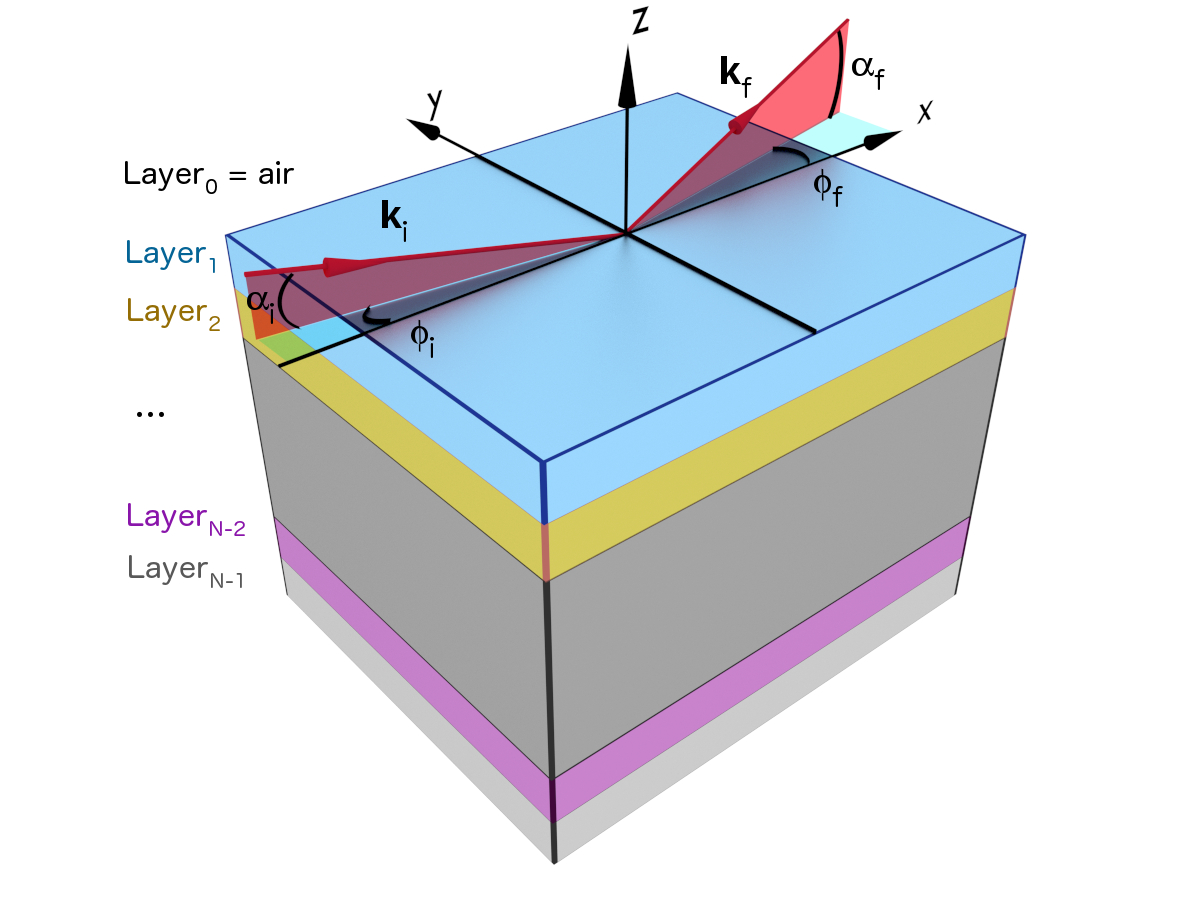
\includegraphics[clip=, width=120mm]{fig/drawing/setup_multilayer.jpg}
  \caption[Conventional GISAS scattering geometry.]{Geometric conventions
\index{Convention!GISAS geometry}%
\index{Grazing-incidence small-angle scattering!geometric conventions}%
\index{Coordinate system!GISAS geometry}%
\index{Glancing angle}%
\index{Scattering!angle}%
\index{Geometry!conventions for GISAS}
  in GISAS scattering comprise a Cartesian coordinate system
  and a set of angles.
  The coordinate system has a $z$ axis normal to the sample plane,
  and pointing into the halfspace where the beam comes from.
  The $x$ axis usually points along the incident beam,
  projected onto the sample plane.
  Incident and final plane waves are characterized
  by wavevectors $\k_\si$, $\k_\sf$;
  the angle $\alpha_\si$ is the incident glancing angle;
  $\phi_\si$ is usually zero, unless used to describe a sample rotation;
  $\alpha_\sf$ is the exit angle with respect to the sample's surface;
  and $\phi_\sf$ is the scattering angle with respect to the scattering plane.
  In the above figure $\phi_\sf$ is negative by convention, while all other angles
  are positive.
\nomenclature[1α024 2i000]{$\alpha_\si$}{Glancing angle of the incident beam}
\nomenclature[1α024 2f000]{$\alpha_\sf$}{Glancing angle of the detected beam}
\nomenclature[1φ024 2i000]{$\phi_\si$}{Angle between the incident beam, projected into the sample plane, and the $x$ axis}%
\nomenclature[1φ024 2f000]{$\phi_\sf$}{Angle between the detected beam, projected into the sample plane, and the $x$ axis}%
\nomenclature[2x020]{$x$}{Horizontal coordinate, usually chosen along the incoming beam projection}%
\nomenclature[2y020]{$y$}{Horizontal oordinate, chosen normal to $z$ and $x$}%
  The numbered layers illustrate a multilayer system as dicussed in \cref{sec:Multilayers}.
\index{Layer!numbering}%
\index{Multilayer}
  }
  \label{fig:expgeom}
\end{figure}
%--------------------------------------------------------------------------------

Reflectometry and grazing-incidence scattering
are designed for the investigation of surfaces, interfaces, and thin layers,
or most generically:
samples with a $2+1$ dimensional structure.
By convention,
we choose the sample surface to lie in the $xy$~plane,
\index{Sample plane}%
and its normal point out of the sample in positive $z$~direction.
\index{Sample normal}%
\nomenclature[2x020]{$x$}{Horizontal coordinate, in the sample plane}%
\nomenclature[2y020]{$y$}{Horizontal coordinate, in the sample plane}%
\nomenclature[2z020]{$z$}{Vertical coordinate, along the sample normal}%
\index{Horizontal plane}%
\index{Vertical direction}%
\index{Convention!horizontal plane}%
\index{Convention!vertical direction}%
In our visualizations, we will always represent the $xy$~plane as \E{horizontal},
and the $z$~axis as upward \E{vertical},
altough there are ``horizontal'' reflectometers
where the sample normal is horizontal in laboratory space.
\index{Reflectometer!vertical vs horizontal}%

Scattering from such systems will be studied in distorted-wave Born approximation.
To determine the neutron scattering cross section~\cref{Exsection},
we need to determine the incident and final wavefunctions
$\psi_\si$ and~$\psi_\sf$.
Vertical variations of the refractive index $n(z)$
\index{Refractive index!vertical variation}%
cause refraction and reflection.
\index{Glancing angle}%
\index{Refraction}%
\index{Reflection}%
For waves propagating at small glancing angles,
the reflectance can take any value between 0 and~1,
even though $1-n$ is only of the order $10^{-5}$ or smaller.
Such zeroth-order effects cannot be accounted for
by perturbative scattering theory.
Instead, we need to deal with refraction and reflection
from the onset, in the wave propagation equation.
Accordingly, the SLD decomposition~\cref{Edecompose_v} takes the form
\begin{equation}\label{Edecompose_vz}
  v(\r) = \mv(z) + \delta v(\r),
\end{equation}
\index{Wave propagation!in multilayer|(}
and the homogeneous wave equation~\cref{EHomoK} becomes
\begin{equation}\label{EWaveZ}
  \left\{\Nabla^2+k(z)^2\right\}\psi(\r) = 0.
\end{equation}
Below and above the sample,
$k(z)=\text{const}$:
in these regions, $\psi(\r)$~is a superposition of plane waves.
The exciting wavefunction is
\index{Exciting wave!DWBA}%
\index{Wave!exciting}%
\begin{equation}\label{Epsiminus}
  \psi_\se(\r) = \e^{i\k_\plll\r_\plll+ik_{\perp\se}z},
\end{equation}
\nomenclature[0$\plll$]{$\plll$}{Parallel to the $xy$ sample plane}%
\nomenclature[0$\perp$]{$\perp$}{Normal to the $xy$ sample plane}%
\nomenclature[2k021\perp]{$k_\perp$}{Component of $\k$ along the sample normal}%
\nomenclature[2k041\plll]{$\k_\plll$}{Projection of $\k$ onto the sample plane}%
The subscripts $\plll$ and~$\perp$ refer to the sample $xy$ plane.
The wavevector components $\k_\plll$ and $k_{\perp}$ must fulfill
\begin{equation}
  k(z)^2=\k_\plll^2+k_{\perp}^2.
\end{equation}
\index{Wavenumber!vertical}%
\index{Vertical wavenumber}%
Continuity across the sample implies
\begin{equation}\label{Ekconst}
  \k_\plll = \text{const}.
\end{equation}
\index{Wavevector!horizontal}%
\index{Horizontal wavevector}%
When the incident wave hits the sample,
it is wholly or partly reflected.
Therefore, the full the solution of~\cref{EWaveZ} in the half space
of the radiation source is
\begin{equation}\label{Eref1}
  \psi(\r) = \e^{i\k_\plll\r_\plll+ik_{\perp\se} z} +
      R\, \e^{i\k_\plll\r_\plll-ik_{\perp\se} z}
\end{equation}
with a complex reflection coefficient~$R$.
\index{Reflection!coefficient}%
The reflected flux is given by the re\-flect\-an\-ce $|R|^2$.
\index{Reflectance}%
\index{Flux!reflected}%
In the opposite halfspace, the solution of~\cref{EWaveZ} is simply
\begin{equation}\label{Etra1}
  \psi(\r) = T\, \e^{i\k_\plll\r_\plll+ik_{\perp\se} z}
\end{equation}
with a complex transmission coefficient~$T$.
The transmitted flux is given by the transmittance $|T|^2$.
\index{Transmittance}%
\index{Flux!transmitted}%

%--------------------------------------------------------------------------------
\begin{figure}[tb]
\begin{center}
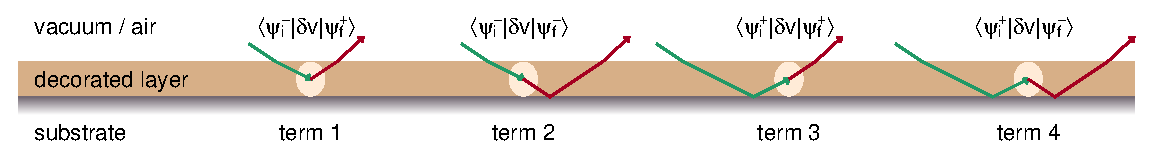
\includegraphics[width=1\textwidth]{fig/drawing/dwba_4terms.ps}
\end{center}
\caption{The four terms in the DWBA scattering matrix element~\cref{Edwba}.
Note that this is a highly simplified visualization.
In particular, it does not show multiple reflections
\index{Multiple reflections}%
\index{Reflection!multiple}%
of incoming or scattered radiation,
though they are properly accounted for by DWBA theory and by all simulation software.}
\label{Fdwba4terms}
\end{figure}
%--------------------------------------------------------------------------------

Within the sample, the wave equation~\cref{EWaveZ}
is solved by the factorization ansatz
\begin{equation}\label{Ekpar}
\psi(\r) = \e^{i \k_\plll\r_\plll} \phi(z).
\end{equation}
\nomenclature[1φ020 0z020]{$\phi(z)$}{$z$-dependent factor of $\psi(\r)$}%
The vertical wavefunction~$\phi(z)$
is governed by the one-dimensional wave equation
\begin{equation}\label{Ewavez}
\left\{\partial_z^2 + k(z)^2 - k_\plll^2 \right\} \phi(z) = 0.
\end{equation}
As solution of a differential equation of second degree,
$\phi(z)$~can be written as superposition
of a downward travelling wave $\phi^-(z)$
and an upward travelling wave $\phi^+(z)$.
Accordingly, the three-dimensional wavefunction can be written as
\begin{equation}\label{Epsisumpm}
  \psi(\r) = \psi^-(\r)+\psi^+(\r).
\end{equation}
\nomenclature[1ψ041 0\pm 2r040]{$\psi^\pm(\r)$}{Upward ($+$) or downward ($-$) propagating component of $\psi(\r)$}%
\nomenclature[0\pm]{$\pm$}{Upward ($+$) or downward ($-$) propagating}%
All this holds not only for the incident wavefunction~$\psi_\si$,
but also for the wavefunction~$\psi_\sf$
that is tracked back from a detector pixel towards the sample.
\index{Backtracking}%
\index{Scattered radiation!backtracking}%
\index{Detector!backtracking}%
Therefore the scattering matrix element
involves two incident and two final partial wavefunctions.
The resulting sum
\index{Wave propagation!in multilayer|)}
\begin{equation}\label{Edwba4}
  \braket{\psi_\si|\delta v|\psi_\sf}
  = \braket{\psi^-_\si|\delta v|\psi^-_\sf}
  + \braket{\psi^-_\si|\delta v|\psi^+_\sf}
  + \braket{\psi^+_\si|\delta v|\psi^-_\sf}
  + \braket{\psi^+_\si|\delta v|\psi^+_\sf}
\end{equation}
is depicted in \Cref{Fdwba4terms}.
It can be written in an obvious shorthand notation
\begin{equation}\label{Edwba}
  \braket{\psi_\si|\delta v|\psi_\sf}
  = \sum_{\pm_\si} \sum_{\pm_\sf}
    \bra{\psi^\pm_\si|\delta v|\psi^\pm_\sf}.
\end{equation}%
This equation contains the essence of
the DWBA for GISAS,
and is the base for all scattering models implemented in \BornAgain.
Since $\braket{\psi_\si|\delta v|\psi_\sf}$
appears as a squared modulus
in the differential cross section~\cref{Exsection},
the four terms of \cref{Edwba} can interfere with each other,
which adds to the complexity of GISAS patterns.

BornAgain supports multilayer samples
with refractive index discontinuities at layer interfaces.
Conventions for layer numbers and interface coordinates are introduced in~\Cref{Fdefz}.
\index{Convention!layer numbering}%
\index{Convention!interface coordinate}%
\index{Coordinate!interface}%
\index{Interface!coordinate}%
\index{Multilayer!numbering}%
\index{Multilayer!coordinates}%
\index{Layer!index}%
\index{Numbering!layers}%
A sample has $N$ layers,
including the semi-infinite bottom and top layers.
Numbering is from top to bottom,
and from 0 to $N-1$ as imposed by the programming languages C$++$ and Python.
Each layer~$l$
\nomenclature[2l010]{$l$}{Layer index}%
has a constant refractive index $n_l$
\nomenclature[2k022 2l010]{$k_l$}{Wavenumber in layer~$l$}%
\nomenclature[2n020 2l010]{$n_l$}{Refractive index of layer~$l$}%
and a constant wavenumber $k_l\coloneqq K_\text{vac} n_l$.
Any up- or downward travelling solution of the wave equation shall be written
as a sum over partial wavefunctions,
\begin{equation}\label{Epsipmsuml}
  \psi^\pm(\r) = \sum_l \psi_l^\pm(\r),
\end{equation}
with the requirement
\begin{equation}\label{Epsipmloutside}
   \psi_l^\pm(\r) = 0 \text{~for $\r$ outside layer~$l$.}
\end{equation}
The DWBA matrix element~\cref{Edwba} then takes the form
\begin{equation}\label{Edwbal}
  \braket{\psi_\si|\delta v|\psi_\sf}
  = \sum_l \sum_{\pm_\si} \sum_{\pm_\sf}
    \braket{\psi^\pm_{\si l}|\delta v|\psi^\pm_{\sf l}}.
\end{equation}

%--------------------------------------------------------------------------------
\begin{figure}[tb]
\begin{center}
\includegraphics[width=0.4\textwidth]{fig/drawing/multilayer_z_conventions.ps}
\end{center}
\caption{Conventions for layer numbers and interface coordinates.
\index{Convention!layer numbering}%
\index{Convention!interface coordinate}%
\index{Coordinate!interface}%
\index{Interface!coordinate}%
\index{Multilayer!numbering}%
\index{Multilayer!coordinates}%
\index{Layer!index}%
\index{Numbering!layers}%
A sample has $N$ layers,
including the semi-infinite bottom and top layers.
\nomenclature[2n120]{$N$}{A multilayer sample has $N$ layers, including the
  semi-infinite bottom and top layers}
Layers are numbered from top to bottom.
The top vacuum (or air) layer (which extends to $z\to+\infty$) has number~0,
the substrate (extending to $z\to-\infty$) is layer~$N-1$.
The parameter $z_l$
\nomenclature[2z020 2l010]{$z_l$}{Vertical
  coordinate at the top of layer~$l$ (at the bottom for $l=0$)}%
is the $z$ coordinate of the \E{top} interface of layer~$l$,
except for $z_0$ which is the coordinate of the \E{bottom} interface
of the air or vacuum layer~0.}
\label{Fdefz}
\end{figure}
%--------------------------------------------------------------------------------

All the above can be easily transcribed to electromagnetic waves.
The scattering matrix element~\cref{EtramaE}
becomes a four-term some over field components $\v{E}^{\pm}_{\text i,f}$.
In full analogy with~\cref{Edwbal},
the sum over layers is
\begin{equation}\label{EdwbalE}
  \braket{\v{E}_\si|\delta v|\v{E}_\sf}
  = \sum_l \sum_{\pm_\si} \sum_{\pm_\sf}
    \braket{\v{E}^\pm_{\si l}|\delta v|\v{E}^\pm_{\sf l}}.
\end{equation}

%%%%%%%%%%%%%%%%%%%%%%%%%%%%%%%%%%%%%%%%%%%%%%%%%%%%%%%%%%%%%%%%%%%%%%%%%%%%%%%%
\section{Homogeneous layers}\label{SLayHomo}
%%%%%%%%%%%%%%%%%%%%%%%%%%%%%%%%%%%%%%%%%%%%%%%%%%%%%%%%%%%%%%%%%%%%%%%%%%%%%%%%

%===============================================================================
\subsection{DWBA for one layer}\label{SStep}
%===============================================================================

BornAgain currently only supports layers with a homogenous matrix.
In terms of~\cref{Edecompose_vz} this means that
$\mv(z)\eqqcolon v_l$ must be constant within a layer.

Within the layer, the directional neutron wavefunction~$\psi^\pm_l$
is a plane wave and factorizes as in~\cref{Ekpar}.
Its amplitude~$A_l^\pm$ is determined recursively
by Fresnel's transmission and reflection coefficients
\index{Fresnel coefficients}%
that are based on continuity conditions at the layer interfaces.
This will be elaborated in \Cref{Sacrolay}.
\index{Multilayer!refractive index profiles}%
\index{Layer!refractive index profiles}%
The vertical wavenumber is determined by \cref{Epsiminus} and~\cref{Ekconst},
\begin{equation}\label{Ekperpl}
  k_{\perp l}^\pm = \pm\sqrt{k_l^2 - k_\plll^2}.
\end{equation}
In the absence of absorption and above the critical angle,
wavevectors are real
so that we can describe the beam in terms of a glancing angle
\begin{equation}\label{Edef_alpha}
  \alpha_l\coloneqq \arctan(k_{\perp l}/k_{\plll}).
\end{equation}
Equivalently,
\begin{equation}\label{Ekplllncos}
  k_{\plll}=K n_l \cos\alpha_l.
\end{equation}
Since $k_{\plll}$ is constant across layers,
we have
\begin{equation}\label{ESnell}
  n_l \cos\alpha_l = \text{the same for all }l,
\end{equation}
which is Snell's refraction law.
\index{Refraction!Snell's law}
\index{Snell's law}
In general, however, the vertical wavenumber $k_{\perp}$,
determined by $k_l$ and $k_\plll$ as per~\cref{Epsiminus},
can become imaginary (total reflection conditions) or complex (absorbing layer).
\index{Wavevector!complex}%
In these cases, glancing angles are no longer well defined,
and the geometric interpretation of~$\psi_l(\r)$ less obvious.
so that one has to fully rely on the algebraic formalism.

With the indicator function
\nomenclature[1χ032 2l010]{$\chi_l(z)$}{Indicates whether $z$ is in layer~$l$}%
\index{Indicator function}%
\begin{equation}\label{Echildef}
  \chi_l(\r)\coloneqq\left\{\begin{array}{ll}
  1&\text{~if $z_l\le z \le z_{l+1}$,}\\[.2ex]
  0&\text{~otherwise,} \end{array}\right.
\end{equation}
the vertical wavefunction can be written
\begin{equation}\label{Ephizwj}
  \phi^\pm_l(z)=A^\pm_l\e^{\pm ik_{\perp l}(z-z_l)}\chi_l(z).
\end{equation}
\nomenclature[2a123 2w010 2l010 \pm]{$A^\pm_{wl}$}{Amplitude
  of the plane wave $\phi^\pm_{wl}(\r)$}%
The offset~$z_l$ has been included in the phase factor for later convenience.

The DWBA transition matrix element~\cref{Edwba} is
\index{Distorted-wave Born approximation!multilayer}%
\begin{equation}\label{Edwba_ml0}
  \braket{\psi_\si|\delta v|\psi_\sf}
  = \sum_l \sum_{\pm_\si} \sum_{\pm_\sf}
    A^{\pm *}_{\si l} A^\pm_{\sf l}
     \delta v_l(\k^\pm_{\sf l}-\k^\pm_{\si l})
\end{equation}
with the Fourier transform of the SLD
restricted to layer~$l$
\begin{equation}\label{Echij}
  \delta v_l(\v{q})
  \coloneqq  \int_{z_l}^{z_{l-1}}\!\d z \int\!\d^2r_\plll\, \e^{i\v{q}\,\r}\delta v(\r)
  = \int\!\d^3r\, \e^{i\v{q}\,\r}\delta v(\r) \chi_l(z).
\end{equation}
\nomenclature[1δ00 2v030 2l010 2q040]{$\delta v_l(\v{q})$}{Fourier transform
of the SLD $\delta v(\r)$, evaluated in one sample layer}%
To alleviate later calculations,
we number the four DWBA terms from 1 to~4 as shown in \cref{Fdwba4terms},
and define the corresponding wavenumbers and amplitude factors and as
\begin{equation}\label{Eudef}
  \begin{array}{l@{\hspace{2em}}l}
    \q^1 \coloneqq  \k^+_\sf - \k^-_\si,& C^1 \coloneqq  A^{-*}_\si A^+_\sf, \\[.6ex]
    \q^2 \coloneqq  \k^-_\sf - \k^-_\si,& C^2 \coloneqq  A^{-*}_\si A^-_\sf, \\[.6ex]
    \q^3 \coloneqq  \k^+_\sf - \k^+_\si,& C^3 \coloneqq  A^{+*}_\si A^+_\sf, \\[.6ex]
    \q^4 \coloneqq  \k^-_\sf - \k^+_\si,& C^4 \coloneqq  A^{+*}_\si A^-_\sf.
  \end{array}
\end{equation}
Accordingly, we can write \cref{Edwba_ml0} as
\begin{equation}\label{Edwba_ml}
  \braket{\psi_\si|\delta v|\psi_\sf}
  = \sum_l \sum_{u} C^u_l \delta v_l(\q_l^u).
\end{equation}
Since $\k_\plll=\text{const}$,
 all wavevectors $\q^u_l$ have the same horizontal component~$\q_\plll$;
they differ only in their vertical component~$q^u_{l\perp}$.

%===============================================================================
\subsection{Wave amplitudes}\label{Sacrolay}
%===============================================================================

\index{Fresnel coefficients}%
\index{Transmission|see {Fresnel coefficients}}%
\index{Reflection|seealso {Fresnel coefficients}}%

The plane-wave amplitudes $A^\pm_{wl}$ need to be computed recursively
from layer to layer.
Since these computations are identical for incident and final waves,
we omit the subscript~$w$ in the remainder of this section.
At layer interfaces, the optical potential changes discontinuously.
From elementary quantum mechanics we know that
piecewise solutions of the Schrödinger equations must be connected
such that the wavefunction $\phi(\r)$ and its first derivative
$\Nabla\phi(\r)$ evolve continuously.

% TODO REPLACE BY TEXT BELOW
\Work{Support for rough interfaces is already implemented in \BornAgain,
but documentation is adjourned to a later edition of this manual.}
%Unless layer interfaces are smooth,
%their roughness causes extra contribution to the total scattering.
%This is implemented in BornAgain as described in \Cref{SRough}.

To deal with the coordinate offsets introduced in \cref{Ephizwj},
we introduce the function%
\begin{equation}\label{Edldef}
  d_l\coloneqq z_l-z_{l+1},
\end{equation}
which is the thickness of layer~$l$,
except for $l=0$,
where the special definition of $z_0$ (\cref{Fdefz}) implies $d_0=0$.
We consider the interface between layers $l$ and $l-1$,
with~$l=1,\ldots,N-1$, as shown in \cref{Fboundary}.
This interface has the vertical coordinate $z_l=z_{l-1}-d_{l-1}$.
Accordingly, the continuity conditions at the interface are
\begin{equation}\label{Econtcond}
  \begin{array}{lcl}
 \hphantom{\partial_z}\phi_l(z_l) &=& \hphantom{\partial_z}\phi_{l-1}(z_{l-1}-d_{l-1}),\\
           \partial_z \phi_l(z_l) &=&           \partial_z \phi_{l-1}(z_{l-1}-d_{l-1}).
  \end{array}
\end{equation}
We abbreviate
\begin{equation}\label{Efldef}
  f_l \coloneqq  k_{\perp l}/K = \sqrt{\overline{n_l^2}-(k_\plll/K)^2}
\end{equation}
and
\begin{equation}\label{Edelldef}
   \delta_l \coloneqq  \e^{iKf_l d_l}.
\end{equation}
For the plane waves \cref{Ephizwj},
the continuity conditions~\cref{Econtcond} take the form
\begin{equation}\label{Econt2}
  \begin{array}{@{}l@{}lcl@{}l}
  +A^-_l &+A^+_l
  &=&
  +A^-_{l-1}\delta_{l-1} &+A^+_{l-1}\delta_{l-1}^{-1},
  \\
  -A^-_l f_l  &+A^+_l f_l
  &=&
  -A^-_{l-1}\delta_{l-1} f_{l-1} &+A^+_{l-1}\delta_{l-1}^{-1} f_{l-1}.
  \end{array}
\end{equation}
After some lines of linear algebra,
we can rewrite this equation system as
\begin{equation}\label{EcMc}
  \left( \begin{array}{c}A^-_{l-1}\\ A^+_{l-1}\end{array} \right)
  = M_l \left( \begin{array}{c}A^-_l\\A^+_l\end{array} \right)
\end{equation}
with the transfer matrix\footnote
{This approach is generally attributed to Abelès,
\index{Abelès matrix}%
who elaborated it in his thesis from 1949, published 1950.
The usually cited paper \cite{Abe50a} is no more than a short advertisement.
Parratt \cite{Par54}, unaware of Abelès, expressed the same relation as a recursion formula.%
\index{Parratt recursion}%
}
\begin{equation}\label{EMil}
  M_l
   \coloneqq
   \left(\begin{array}{cc}
     \delta_{l-1}^{-1}&0\\
       0 & \delta_{l-1}
   \end{array}\right)
   \frac{1}{2f_{l-1}}
   \left(\begin{array}{cc}
       (f_{l-1}+f_l)&(f_{l-1}-f_l)\\
       (f_{l-1}-f_l)&(f_{l-1}+f_l)
   \end{array}\right).
\end{equation}

%--------------------------------------------------------------------------------
\begin{figure}[tb]
\begin{center}
\includegraphics[width=0.46\textwidth]{fig/drawing/multilayer_boundary.ps}
\end{center}
\caption{The transfer matrix $M_l$ connects the wavefunctions
\index{Multilayer!transfer matrix}%
\index{Layer!transfer matrix}%
\index{Transfer matrix}%
$\Phi_l$, $\Phi_{l-1}$ in adjacent layers.}
\label{Fboundary}
\end{figure}
%--------------------------------------------------------------------------------

In a scattering setup,
plane-wave amplitudes are subject to two boundary conditions.
Let us assume that the source or the sink is located at $z>0$.
Then in the top layer, $A^-_{0}=1$ is given by the
incident or back-traced final plane wave.
In the substrate, $A^+_{N-1}=0$ because there is no radiation
coming from $z\to-\infty$.
This leaves us with two unkown amplitudes,
the overall coefficients of transmission~$A^-_{N-1}$ and reflection~$A^+_0$.
These two unknowns are connected by a system of two linear equations,
\begin{equation}\label{E1Ap}
  \left( \begin{array}{c}1\\ A^+_0\end{array} \right)
  = M_1 \cdots M_{N-1} \left( \begin{array}{c}A^-_{N-1}\\0\end{array} \right).
\end{equation}
While it is possible in principle
to solve this as a matrix equation,
the actual implementation in \BornAgain\footnote
{In file \SRC{Core/Multilayer}{SpecularMatrix.cpp}, function \T{SpecularMatrix::execute}.}
starts with a unit vector in the substrate,
and then carries out the propagation step \cref{EcMc}
interface by interface,
yielding unnormalized amplitudes
\begin{equation}\label{EAtildel}
  \left( \begin{array}{c}\tilde A^-_l\\ \tilde A^+_l\end{array} \right)
  \coloneqq M_{l+1}\cdots M_{N-1} \left( \begin{array}{c}1\\0\end{array} \right).
\end{equation}
When the top layer is reached,
the obtained values are normalized
so that the boundary condition $A^-_{0}=1$ be satisfied,
\begin{equation}\label{EApml}
  A^\pm_l = \frac{\tilde A^\pm_l}{\tilde A^-_0}.
\end{equation}
For GISAS detection in transmission geometry
\index{Transmission geometry}%
\index{Detector!transmission geometry}%
(sink location $z<0$) all the development
following \cref{EMil} holds with exchanged order of layers:
$(0,\ldots, N-1) \mapsto (N-1,\ldots,0)$.

\Work{GISAS in transmission geometry is not yet implemented in \BornAgain,
  but high on our agenda.}

The above algorithm fails if $f_l\to0$
because $M_{l+1}$ becomes singular.
The general solution of \cref{Ewavez} will be a linear function of $z$:
\begin{equation}\label{Ephilz}
  \phi_l(z) = A^0_l + A^1_lz.
\end{equation}
In \BornAgain, such a linear wavefunction amplitude can not be handled by the form factors,
which are only defined in terms of plane waves with complex wavevector components.
The following cases are treated seperately:
\begin{itemize}
  \item There is only one layer: this is a trivial case whithout any need to calculate wave coefficients.
    The solution in the single layer is just the incoming/outgoing plane wave.
  \item The top layer of a multilayer has $f_0=0$: the limit $f_0\to0$ is well-defined and the
    solution is given by $A^+_0 = -A^-_0$ and $A^{\pm}_l=0$ for $l>0$.
    % The boundary condition in the substrate imposes a linear relation between the two coefficients
    % of the linear wavefunction amplitude in the top layer. Since the first order term has to vanish, all amplitudes vanish.
  \item $f_l=0$ for a layer with $l>0$: In this case $f_l$ will be given a very small imaginary value,
    representing a slight absorption. However, this should be inconsequential because the index of refraction
    of non-vacuum layer always contains an absorptive component.
\end{itemize}

%===============================================================================
\subsection{Flux, evanescent waves}\label{SSpecial}
%===============================================================================

We write
\begin{equation}\label{Edecompkperp}
  k_\perp \eqqcolon k_\perp' + i k_\perp''
\end{equation}
for the decomposition into a real and an imaginary part.
Accordingly, full wavevectors have the decomposition
\begin{equation}
  \k^\pm
  \eqqcolon {\k^\pm}' + i{\k^\pm}''
  = \k_\plll \pm (k_\perp' + i k_\perp'')\v{\hat z}.
\end{equation}
Per \cref{Endb1}, we have $\beta\ge0$ and $\delta<1$,
from which it follows that $k_\perp''$ always has the same sign as $k_\perp'$.

After these preparations,
we can compute the flux~\cref{EdefJ}:
\begin{equation}\label{EJ1}
  \begin{array}{@{}l@{\;}l}
  \v{J}(\r)
  =&   \left|A^-\right|^2 \e^{+2k_\perp'' (z-z_l)} {\k^-}'
    + \left|A^+\right|^2 \e^{-2k_\perp''(z-z_l)} {\k^+}'
\\[2ex]
  &+ \left[
      A^-{A^+}^* \e^{-2ik_\perp'(z-z_l)} {\left(\k_\plll-ik_\perp''\v{\hat z}\right)}
    + \text{c.c.}
    \right].
  \end{array}
\end{equation}
The first two terms describe the exponential intensity decrease
due to absorption, while
the oscillatory term in square brackets
is responsible for waveguide effects in layers with finite thickness.
The flux can also be written in terms of the one-dimensional wavefunctions $\phi^{\pm}(z)$:
\begin{equation}\label{EJ2}
  \begin{array}{@{}l@{\;}l}
  \v{J}(\r) =& \left|\phi^+(z)+\phi^-(z)\right|^2\cdot\k_\plll \\
  &+ \left[ \left|\phi^+(z)\right|^2 k_\perp' - \left|\phi^-(z)\right|^2 k_\perp' +
  2\Im(\phi^-(z){\phi^+}^*(z))k_\perp'' \right]\cdot \v{\hat z}.
  \end{array}
\end{equation}
The first term denotes the horizontal component
of the flux and can be seen to consist of the product
of the particle density at position $z$ and the wavector $\k_\plll$.
The $z$-component consists of the difference
between the up- and downward travelling wave components
and an extra term that encodes the interference between them.

In the special case of a purely imaginary~$k_{\perp l}$,
the flux becomes:
\begin{equation}\label{EJ3}
  \v{J}(\r) = \left| \psi \right|^2 \k_\plll + 2 \Im (A^-{A^+}^*) k_\perp''\v{\hat z}.
\end{equation}
This flux consists of two clearly distinct parts: an \E{evanescent wave},
\index{Evanescent wave}%
travelling horizontally
 and a vertical component that is independent of the $z$ position.
The vertical component is a necessary
 degree of freedom to fulfill the boundary conditions at the layer's top and bottom interfaces.
In the case of a semi-infinite layer, the vertical component becomes zero and
 all incoming radiation at the top of the layer undergoes \E{total reflection}.
\index{Total reflection}%

%===============================================================================
\subsection{Modifications for X-rays}\label{SmulayX}
%===============================================================================

\def\Ep{\v{\Phi}}
\def\hn{\v{n}}

We shall now translate the above results from unpolarized neutrons to X-rays.
The vectorial amplitude of the electromagnetic field will require
nontrivial modifications.
In place of the factorization~\cref{Ekpar}, we write
\begin{equation}
  \v{E}(\r)=\e^{i\k_\plll\r}\Ep(z).
\end{equation}
In place of~\cref{Ephizwj},
the vertical wavefunction is
\begin{equation}
  \Ep^\pm_l(z) = \v{A}^\pm_l \e^{\pm ik_\perp(z-z_l)}\chi_l(z).
\end{equation}

%--------------------------------------------------------------------------------
\begin{figure}[tb]
\begin{center}
\includegraphics[width=0.8\textwidth]{fig/drawing/s-vs-p-polarization.ps}
\end{center}
\caption{Conventions for polarization directions relative to a refracting interface:
\index{Convention!p- and s-polarization}%
\index{Polarization!p and s@$p$ and $s$}%
\index{p Polarization@$p$-Polarization}%
\index{s Polarization@$s$-Polarization}%
For $p$ polarization, the electric field vector~$\v{E}$ is parallel to the interface normal~$\hn$;
for $s$ polarization, it is perpendicular (\E{senkrecht} in German).
In either case, $\v{E}$ is perpendicular to the wavevector~$\k$.}
\label{Fsppol}
\end{figure}
%--------------------------------------------------------------------------------

The vectorial character of $\v{A}^\pm_{wl}$ will require changes in~\cref{Sacrolay}.
For electromagnetic radiation in nonmagnetic media,
the boundary conditions at an interface with normal $\hn$ are \cite[eq. 7.37]{Jac75}
% , Born \& Wolf \cite[ch.~1.1.3]{BoWo99}, or Hecht \cite[ch.~4.6.1]{Hec02}.}
\nomenclature[2n04]{$\hn$}{Normal vector of an interface}
\begin{align}
  &\sum_\pm\,\overline{\epsilon}\,\v{E}^\pm\,\hn = \text{const}, \label{EbcE1}\\[1.4ex]
  &\sum_\pm\,\v{E}^\pm\times\hn = \text{const}, \label{EbcE2}\\[1.4ex]
  &\sum_\pm\,\k^\pm_l\times\v{E}^\pm = \text{const}. \label{EbcE3}
\end{align}
We will only consider the two polarization directions,
\index{Convention!p- and s-polarization}%
\index{Polarization!p and s@$p$ and $s$}%
\index{p Polarization@$p$-Polarization}%
\index{s Polarization@$s$-Polarization}%
conventionally designated as $p$ and~$s$, defined in \Cref{Fsppol}.
As some algebra on \cref{EbcE1,EbcE2,EbcE3} would show,
these are \E{principal axes},
meaning that if both incoming fields $\v{E}^-_{l-1}$ and~$\v{E}^+_l$ are strictly
polarized in either $p$ or $s$ direction,
then the outgoing fields $\v{E}^+_{l-1}$ and~$\v{E}^-_l$
are polarized in the same direction.
Conversely, if the incoming fields are mixtures of $p$ and $s$ polarization,
then the outgoing fields will be, in general, mixed differently.
Therefore if polarization factors are quantitatively important in an experiment,
one should strive to accurately polarize the incident beam in $p$ or $s$ direction
in order to avoid the extra complication of variably mixed polarizations.

Further algebra on \cref{EbcE1,EbcE2,EbcE3} replicates the
reflection law that relates $\k^-$ and $k^+$
and Snell's law~\cref{ESnell}.
Taking these for granted,
we only retain equations that are needed to determine the field amplitudes~$E^\pm$.
For $p$~polarization they yield
\begin{equation}
  \left(\begin{array}{cc}k&k\\
       -k_\perp/k&k_\perp/k\end{array}\right)
  \left(\begin{array}{c}E^-\\
       E^+\end{array}\right) = \text{const},
\end{equation}
and for $s$~polarization
\begin{equation}
  \left(\begin{array}{cc}1&1\\
       -k_\perp&k_\perp\end{array}\right)
  \left(\begin{array}{c}E^-\\
       E^+\end{array}\right) = \text{const}.
\end{equation}
The latter equation can be brought into the form~\cref{Econt2}.
In consequence,
$s$-polarized X-rays are refracted and reflected in
exactly the same ways as unpolarized neutrons.
For $p$ polarization, the transfer matrix~\cref{EMil}
must be replaced by
\begin{equation}
  M_l^{\text(p)} = TODO,
\end{equation}
\Work{In BornAgain, this modified transfer matrix is not yet implemented;
only $s$ polarized X-rays are currently supported.}

\Work{The following paragraph on polarization factors shall be worked out next:}
In $s$~geometry the coefficients $C^u_l$ of \Cref{Edwba_mlE}
are given by simple products of scalar amplitudes as in~\cref{Eudef}.

The DWBA matrix element is
\begin{equation}\label{Edwba_mlE}
  \braket{\v{E}_\si|\delta v|\v{E}_\sf}
  = \sum_l \sum_{u} C^u_l \delta v_l(\q_l^u).
\end{equation}
in full analogy with~\cref{Edwba_ml},
but the coefficients are now scalar products
$C^1=\v{A}^{-*}_\si\v{A}^{+}_\sf$ etc.\ instead of the products of scalar factors in~\cref{Eudef}.

and the coefficients of \Cref{Edwba_mlE} are
\begin{equation}
  \begin{array}{@{}lcl}
    C^1 &=& A^{-*}_\si A^+_\sf,\\
    C^2 &=& A^{-*}_\si A^-_\sf\cos(\alpha_-+\alpha_+),\\
    C^3 &=& A^{+*}_\si A^+_\sf\cos(\alpha_-+\alpha_+),\\
    C^4 &=& A^{+*}_\si A^-_\sf.
  \end{array}
\end{equation}
\Work{In BornAgain, polarization factors are not yet implemented.}


%===============================================================================
\iffalse
\section{Graded refractive index}\label{Sgraded}
%===============================================================================

\Cref{Ewavez} has no practicable solution for arbitrary functions~$k(z)$.

Within one layer, the refractive index must either be constant,
or have an affine linear dependence $n(z)^2=a+bz$.
All other cases must be handled by dividing the sample into many layers
and approximating $n(z)^2$ by a step function.

\Work{Support for linear gradings with $n(z)^2=a+bz$ is not yet implemented.}
\index{Refractive index!graded}%
\index{Graded layer}%
\index{Layer!graded}%

For a graded refractive index~$n$
 that is a smooth function of~$z$,
the differential equation~\cref{Ewavez} is best solved
using the WKB method.\footnote
{Also called \E{semiclassical approximation} or
\E{phase integral method},
%originally developed
%by Liouville (1837), Green (1837), Lord Rayleigh (1912), and Jeffreys (1923),
named after Wentzel (1926), Kramers (1926), Brillouin (1926).
See any textbook on quantum mechanics.}
\index{WKB method}%
\index{Semiclassical approximation|see {WKB method}}%
\index{Phase integral method|see {WKB method}}%

\fi

\index{Multilayer|)}%

%%%%%%%%%%%%%%%%%%%%%%%%%%%%%%%%%%%%%%%%%%%%%%%%%%%%%%%%%%%%%%%%%%%%%%%%%%%%%%%%
%%
%%   BornAgain User Manual
%%
%%   homepage:   http://www.bornagainproject.org
%%
%%   copyright:  Forschungszentrum Jülich GmbH 2015
%%
%%   license:    Creative Commons CC-BY-SA
%%   
%%   authors:    Scientific Computing Group at MLZ Garching
%%               C. Durniak, M. Ganeva, G. Pospelov, W. Van Herck, J. Wuttke
%%
%%%%%%%%%%%%%%%%%%%%%%%%%%%%%%%%%%%%%%%%%%%%%%%%%%%%%%%%%%%%%%%%%%%%%%%%%%%%%%%%


\chapter{Particle Assemblies}  \label{sec:Assemblies}


%%%%%%%%%%%%%%%%%%%%%%%%%%%%%%%%%%%%%%%%%%%%%%%%%%%%%%%%%%%%%%%%%%%%%%%%%%%%%%%%
\section{Particle distributions}
%%%%%%%%%%%%%%%%%%%%%%%%%%%%%%%%%%%%%%%%%%%%%%%%%%%%%%%%%%%%%%%%%%%%%%%%%%%%%%%%

In the previous chapter we discussed the form factor of isolated
nano- or meso-particles.
Unless these particles are dilute like an ideal gas,
their positions are somehow correlated,
which leads to interference patterns in the scattered radiation.
In the following,
we present particle assembly models that are supported in \BornAgain.
For a more complete theoretical description,
the user is referred to, for example, reference~\cite{ReLL09}.

%===============================================================================
\subsection{Collection of particles} \label{sec:sect:interf}
%===============================================================================

Let us consider the general geometry of a scattering experiment. An incident neutron with a wave vector $\k_\text{i}$ is scattered in a new direction $\k_\text{f}$ after interacting with a particle. This scattering occurs in a cone of solid angle $d\Omega$ around the direction of the scattered wave vector $\k_\text{f}$.
Considering a set of $N$ particles labeled with index $i$, located at $\r_i$ and having shapes $S_i(\r)$ ($S_i=0$ outside the particle and 1 inside), occupying a total volume $V$, the differential cross-section per particle is given by:
\begin{equation*}
  \frac{d\sigma}{d\Omega}(\q) = \frac{1}{N}\left\lbrace \sum_i \left\lvert F_i(\q) \right\rvert ^2 + \sum_{i\neq j} F_i(\q) F_{j}^*(\q) \exp \left[i\q\cdot (\v{R}_i-\v{R}_j)\right] \right\rbrace.
\end{equation*}
where  $\q=\k_\text{i} - \k_\text{f}$ is the wave vector transfer and $F_i$ is the form factor of particle $i$ (see Sect.~\ref{sec:sect:ff} for a description).

Since in most experimental conditions only the statistical properties of the particles are known, one can consider the probabilistic value of this cross-section \textit{i.e.} its expectation value. Assuming that the particles' shapes are determined by their class $\alpha$, with the abundance ratio $p_\alpha \equiv N_\alpha / N$, and defining the particle density as $\rho_V \equiv N/V$, the expectation value becomes:
\begin{align*}
  \bra \frac{d\sigma}{d\Omega}(\q) \ket  & = \sum_\alpha p_\alpha \left\lvert F_\alpha(\q)\right\rvert ^2 + \frac{\rho_V}{V}\sum_{\alpha,\beta} p_\alpha p_\beta F_\alpha (\q)F_\beta^*(\q)  \\
  & \times \iint_V d^3\v{R}_\alpha d^3\v{R}_\beta \ppcf{\alpha}{\beta}{R} \exp \left[ i\q\cdot (\v{R}_\alpha - \v{R}_\beta ) \right],
\end{align*}

where $\ppcf{\alpha}{\beta}{R}$ is called the \emph{partial pair correlation function}. It represents the normalized probability of finding particles of type $\alpha$ and $\beta$ in positions $\v{R}_\alpha$ and $\v{R}_\beta$ respectively. 

TO MERGE IN:
This expression can be split into a diffuse part, which by definition should be zero for the case of only one particle type, and a coherent part, resulting from the coherent superposition of scattering amplitudes for particles at different positions:
\begin{equation*}
  \bra \frac{d\sigma}{d\Omega}(\q) \ket
  = I_d(\q) + {\bra F_\alpha (\q ) S_{\alpha\beta} (\q) F_\beta^* (\q)
               \ket}_{\alpha\beta},
\end{equation*}
where
\begin{align*}
  I_d(\q) &
  \equiv {\bra\left\rvert F_\alpha (\q) \right\rvert^2\ket}_{\alpha}
       - \left\lvert {\bra F_\alpha (\q)\ket}_{\alpha} \right\rvert^2, \\
  S_{\alpha\beta} (\q) &\equiv 1 + \rho_V \int_V d^3\r\mathcal{G}_{\alpha\beta}(\r) \exp \left[ i\q\cdot \r \right].
\end{align*}
$S_{\alpha\beta} (\q)$ is called the \emph{interference function} and $\bra\dotso\ket_\alpha$ is the expectation value over the classes $\lbrace \alpha\rbrace$.


TO MERGE IN:
More precisely, the probability density for finding a particle $\alpha$ at position $\v{R}_\alpha$ and another one of type $\beta$ at $\v{R}_\beta$ is given by:
\begin{equation*}
  \mathcal{P}(\alpha, \v{R}_\alpha ; \beta , \v{R}_\beta ) \equiv \rho_V^2 p_\alpha p_\beta \ppcf{\alpha}{\beta}{R}.
\end{equation*}


%===============================================================================
\section{Horizontal particle distributions}
%===============================================================================

To proceed further, when the morphology and topology are not exactly known, some hypotheses need to be made since the correlation between the kinds of scatterers and their relative positions included in the pair correlation functions are difficult to estimate. Several options are available:

\paragraph{Decoupling approximation (DA)}
\index{Decoupling approximation}
neglects all correlations. It supposes that the particles are positioned in a way that is completely independent on their kinds (shapes, sizes). An example is given in figure~\ref{fig:da}. Thus the kind of scattering objects and their positions are not correlated and the partial pair correlation function is independent of the particle class $\alpha$. We can therefore replace $ \ppcfb{\alpha}{\beta}{R}$ by  $g(\v{R}_{\alpha\beta})$.

This leads to the following expression of the scattering cross-section:
\begin{equation*}
\bra \frac{d\sigma}{d\Omega}(\q) \ket  = I_d(\q) + \left\lvert \bra F_\alpha(\q) \ket_\alpha \right\rvert ^2 \times S(\q),
\end{equation*}
where $I_d$ is the diffuse part of the scattering. It is the signature of the fluctuations of shapes, sizes or orientations of the particles; its maximum is located in $q_{\parallel}=0$. In the second term of the expression of the scattering cross-section, $S(\q)$ is the interference function and is given by
\begin{equation*} 
  S(\q) = 1+ \rho_V \int_V d^3\r g(\r) \exp \left[ i\q\cdot \r \right].
\end{equation*}


\begin{figure}[ht]
\begin{center}
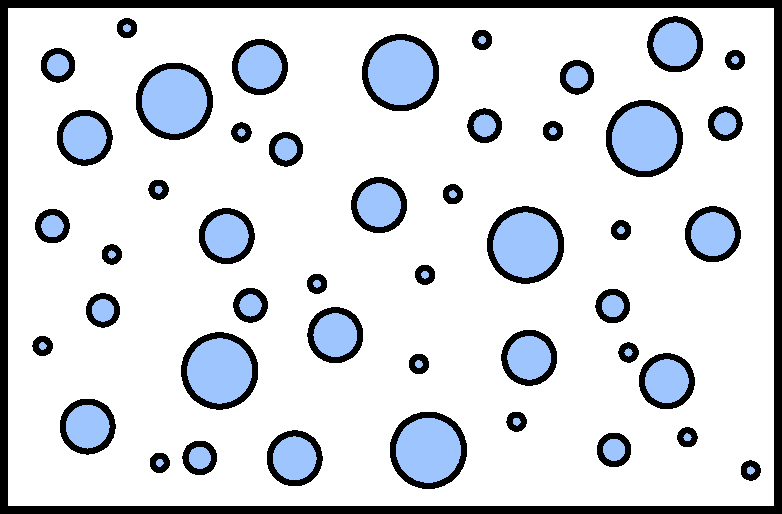
\includegraphics[width=0.5\textwidth]{fig/drawing/drawingDA.pdf}
\end{center}
\caption{Sketch of a collection of particles deposited on a substrate whose scattering  could be described by the decoupling approximation.}
\label{fig:da}
\end{figure}


In concentrated systems, DA breaks down because of correlations. One solution is to reintroduce some correlations between particles sizes and distributions using, for example, the size spacing correlation approximation described below. 

\paragraph{Local monodisperse approximation (LMA)}
\index{Local monodisperse approximation}
partially accounts for some coupling between the positions and the kinds of the particles \cite{Ped94}. 
 It requires a subdivision of the layers of particles into monodisperse domains. The contributions of these subdomains are then  incoherently summed up and weighted by the size-shape probabilities.\\ In this approximation, a particle is supposed to be surrounded by particles of the same size and shape, within the coherence length of the input beam (see fig.~\ref{fig:lma}). The scattering cross-section is expressed as
\begin{equation*}
  \bra \frac{d\sigma}{d\Omega}(\q) \ket \simeq \bra \left\lvert F_\alpha(\q)\right\rvert ^2 S_\alpha(\q) \ket_\alpha.
\end{equation*}

Contrary to the Decoupling Approximation, the Local Monodisperse Approximation can account for particle class/size/shape-dependent pair correlation functions by having distinct interference functions $S_\alpha(\q)$.

One has to remember that in most cases, this approximation corresponds to an unphysical description of the investigated systems. \\ 

DA and LMA separate the contributions of the form factors and of the interference function. For disordered systems DA and LMA give the same result as the scattering vector gets larger \textit{i.e.} the scattered intensity is dominated by the contribution of the form factor.

\begin{figure}[ht]
\begin{center}
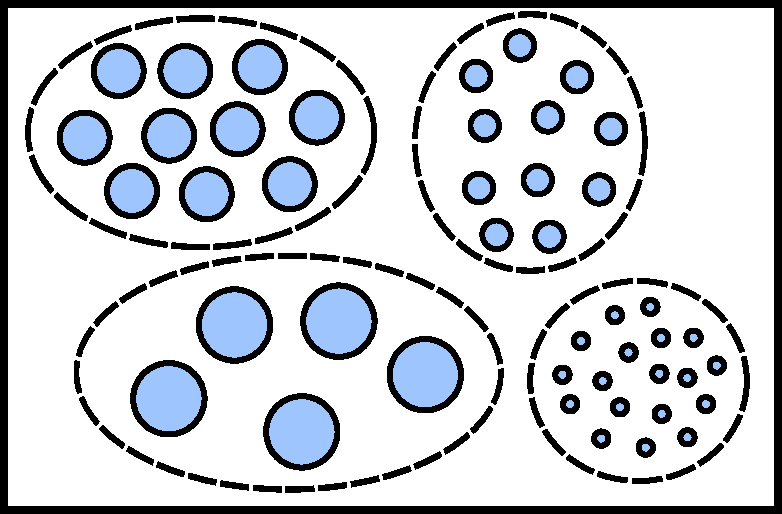
\includegraphics[width=0.5\textwidth]{fig/drawing/drawingLMA.pdf}
\end{center}
\caption{Sketch of a collection of particles deposited on a substrate whose scattering could be described by the local monodisperse correlation approximation. The dashed areas mark the coherent domains. In this case, the total scattering intensity is the incoherent sum from all these domains.}
\label{fig:lma}
\end{figure}



\MakeRemark{Terminology}{
\\
For collections of particles, the scattered intensity contains contributions from neighboring particles. This additional pattern can be called the structure factor, the interference function or even in crystallography, the lattice factor. In this manual, we use the term "interference function" or interferences.
}


%===============================================================================
\subsection{Layout of particles}\label{sec:partlayout}
%===============================================================================

\subsubsection{The uncorrelated or disordered lattice}
For very diluted distributions of particles, the particles are too far apart from each other to lead to any interference between the waves scattered by each of them. In this case the interference function is equal to 1. The scattered intensity is then entirely determined by the form factors of the particles distributed in the sample.

\subsubsection{The regular  lattice}\mbox{}\\
The particles are positioned at regular intervals generating a layout characterized by its base vectors $\mathbf{a}$ and $\mathbf{b}$ (in direct space) and the angle between these two vectors.
This lattice can be two or one-dimensional depending on the characteristics of the particles. For example when they are infinitely long, the implementation can be simplified and reduced to a "pseudo" 1D system.

\paragraph{The ideal paracrystal} \mbox{}\\
\index{Paracrystal}
A paracrystal, whose notion was developed by Hosemann\cite{Hos51}, allows fluctuations of the lengths and orientations of lattice vectors. Paracrystals can be defined as distorted crystals in which the crystalline order has not disappeared and for which the behavior of the interference functions  at small angles is coherent.
It is a transition between the regular lattice and the disordered state.\\

For example, in one dimension, a paracrystal is generated using the following method. First we place a particle at the origin. The second particle is put at a distance $x$ with a density probability $p(x)$ that is peaked at a mean value $D$: $\int_{-\infty} ^{\infty}p(x)dx=1$ and $\int_{-\infty}^{\infty}xp(x)dx=D$. The third one is added at a distance $y$ from the second site using the same rule with a density probability $p_2(y)= \int_{-\infty}^{\infty}p(x)p(y-x)dx=p\otimes p(y)$.\\ With such a method, the pair correlation function $g(x)$ is built step by step. Its expression and the one of its Fourier transform, which is the interference function are 
\begin{equation*}
g(x)=\delta(x)+ p(x)+ p(x)\otimes p(x)+\ldots + p(-x)+\ldots \: \mathrm{and}\:\, S(q)=\Re\left(\dfrac{1+P(q)}{1-P(q)}\right),
\end{equation*}
 where $P(q)$ is the Fourier transform of the density probability $p(x)$.\\

\paragraph{Example} For a probability distribution function is Gaussian:
\begin{equation*}
p(x)=\frac{1}{\omega \sqrt{2\pi}} \exp\left(-\dfrac{(x-D)^2}{\omega^2}\right),\qquad P(q)=\exp\left(-\frac{q^2 \omega^2}{2}\right)\exp(iqD).
\end{equation*}
 The interference function of a one-dimensional paracrystal is given by

\begin{align*}
S(q) =\Re \left(\frac{1+\Phi(q) }{1 - \Phi(q)} \right), \quad \mathrm{where}\quad \Phi(q) = P(q)\exp\left(-\frac{D}{\Lambda}\right),
\end{align*}
where $\Lambda$ is a damping length used in order to introduce some finite-size effects.

Figure~\ref{fig:1dparas_q} shows the evolution of $S(q)$ for different values of $\omega /D$. 

\begin{figure}[ht]
\begin{center}
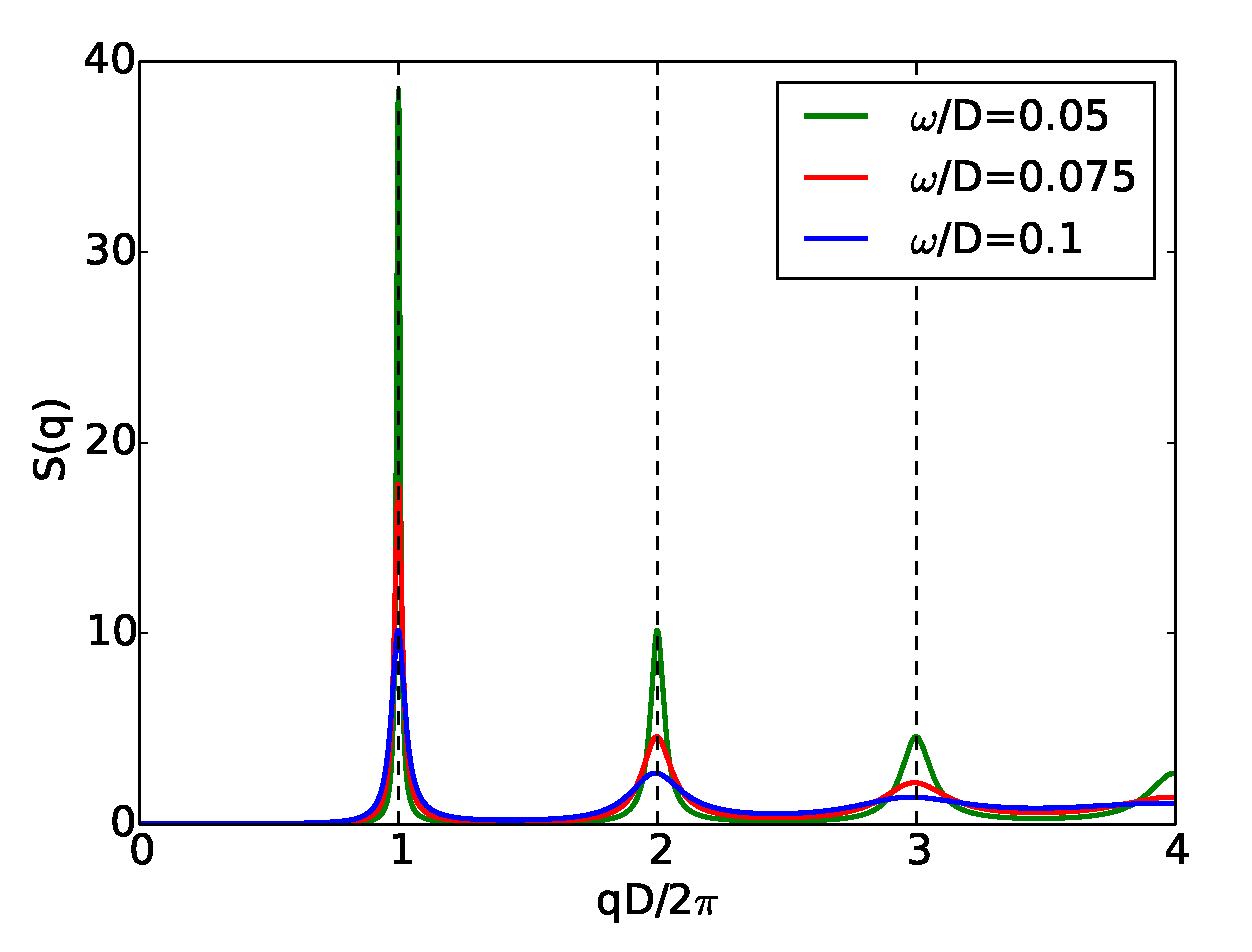
\includegraphics[width=0.6\textwidth]{fig/funcplot/S_q_1Dparacrystal.eps}
\end{center}
\caption{Interference function of a 1D Gaussian paracrystal plotted for different values of $\omega /D$. The peaks broaden with a decreasing amplitude as $\omega/D$ increases. This shows the transition between an ordered and a disordered states. }
\label{fig:1dparas_q}
\end{figure}

In two dimensions, the paracrystal is constructed on a pseudo-regular lattice with base vectors $\mathbf{a}$ and $\mathbf{b}$ using the following conditions for the densities of probabilities:\\ $\int p_{\mathbf{a}}(\r)d^2\r=\int p_{\mathbf{b}}(\r)d^2\r=1$, $\int \r p_{\mathbf{a}}(\r)d^2\r=\mathbf{a}$, $\int \r p_{\mathbf{b}}(\r)d^2\r=\mathbf{b}$.\\
In the ideal case the deformations along the two axes are decoupled and each unit cell should retain a parallelogram shape. The interference function is given by\\ $S(q_{\parallel})=\prod_{k=a,b}\Re\left(\dfrac{1+P_k(q_{\parallel})}{1-P_k(q_{\parallel})} \right)$ with $P_k$ the Fourier transform of $p_k$, $k=a, b$.

\paragraph{Probability distributions} \mbox{}\\
The scattering by an ordered lattice gives rise to a series of Bragg peaks situated at the nodes of the reciprocal lattice. Any divergence from the ideal crystalline case modifies the output spectrum by, for example, widening or attenuating the Bragg peaks. The influence of these "defects" can be accounted for 
 in direct space by using correlation functions or by truncating the lattice or, in reciprocal space with structure factors or interference functions by convoluting the scattered peaks with a function which could reproduce the experimental shapes.



%===============================================================================
\subsubsection{Size-Spacing Correlation Approximation}
%===============================================================================
\index{Size-spacing correlation approximation}
\index{SSCA|see {Size-spacing correlation approximation}}

TO MERGE IN:
introduces correlations between polydisperse particles, more precisely between the size of the particles and their mutual spacing. A classical example would consist in particles whose closest-neighbor spacing depends linearly on the sum of their respective sizes \cite{LaLR07}, as illustrated in fig.~\ref{fig:ssca}.

%For a sample where only the statistical properties of particle positions and size are known, the scattered intensity per scattering particle is expressed as the average over an ensemble of the Fourier transform of the Patterson function, which is the autocorrelation of the scattering length density $\curlp (\r ) \equiv \sum_{ij} S_i(-\r )\otimes S_j(\r )\otimes \delta (\r + \r_i - \r_j )$:
%\begin{equation*}
%  I(\q ) = \frac{1}{N}\ensavg{}{\curlf (\curlp (\r ))},
%\end{equation*}
%where $\curlf$ denotes the Fourier transform and $\curlp$ the Patterson function

\begin{figure}[ht]
\begin{center}
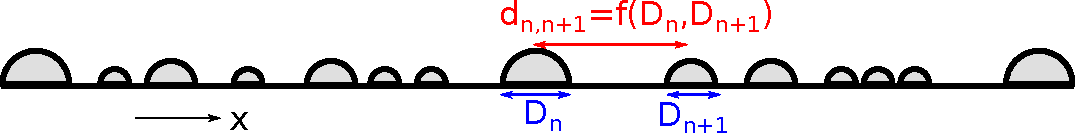
\includegraphics[width=0.9\textwidth]{fig/drawing/drawingSSCA.pdf}
\end{center}
\caption{Sketch of a 1D distributed collection of particles, whose scattering could be described by the size-spacing correlation approximation: the distance between two particles depends on their sizes.}
\label{fig:ssca}
\end{figure}


In the Size-Spacing Correlation Approximation, a correlation is assumed between the shape/size of the particles and their mutual spacing. A classical example would consist of particles whose closest-neighbor spacing depends linearly on the sum of their respective sizes. The following discussion of this type of correlation is inspired by \cite{LaLR07}

The scattered intensity can also be calculated as the Fourier transform of the Patterson function, which is the autocorrelation of the scattering length density:
\begin{equation*}
  \curlp (\r ) \equiv \sum_{ij} S_i(-\r )\otimes S_j(\r )\otimes \delta (\r + \r_i - \r_j ).
\end{equation*}
For a sample where only the statistical properties of particle positions and shape/size are known, the scattered intensity per scattering particle becomes average over an ensemble of the Fourier transform of the Patterson function:
\begin{equation*}
  I(\q ) = \frac{1}{N}\bra\curlf (\curlp (\r ))\ket,
\end{equation*}
where $\curlf$ denotes the Fourier transform.

The ensemble averaged Patterson function will be denoted as:
\begin{equation*}
  Z(r) \equiv \frac{1}{N}\bra\curlp (\r )\ket.
\end{equation*}
In the case of systems where the particles are aligned in one dimension, this autocorrelation function can be further split into nearest neighbor probabilities. First, it is split into terms for negative, zero or positive distance:
\begin{equation*}
  Z(\r ) \equiv z_0(\r ) + z_+(\r ) + z_-(\r ).
\end{equation*}
Taking $x$ as the coordinate in the direction in which the particles are arranged and $s$ as an orthogonal coordinate ($\r \equiv (x,s)$), one obtains:
BROKEN TODO RESTORE
\iffalse
\begin{align*}
  z_0(\r ) &= \sum_{\alpha_0} p(\alpha_0) S_{\alpha_0}(-x,-s) \otimes S_{\alpha_0}(x,s)  \\
  z_+(\r ) &= \sum_{\alpha_0\alpha_1} p(\alpha_0,\alpha_1) S_{\alpha_0}(-x,-s) \otimes S_{\alpha_1}(x,s) \otimes P_1(x|\alpha_0\alpha_1)  \\
               &+ \sum_{\alpha_0\alpha_1\alpha_2} p(\alpha_0,\alpha_1,\alpha_2) S_{\alpha_0}(-x,-s) \otimes S_{\alpha_2}(x,s) \otimes P_1(x|\alpha_0\alpha_1) \otimes P_2(x|\alpha_0\alpha_1\alpha_2)  \\
               &+ \dotsb \\
  z_-(\r ) &= z_+(-\r ),
\end{align*}
\fi
where $p(\alpha_0,\dotsc ,\alpha_n)$ denotes the probability of having a sequence of particles of the indicated sizes/shapes and $P_n(x|\alpha_0\dotsc\alpha_n)$ is the probability density of having a particle of type $\alpha_n$ at a (positive) distance $x$ of its nearest neighbor of type $\alpha_{n-1}$ in a sequence of the given order.

In the Size-Spacing Correlation Approximation, one assumes that the particle sequence probabilities are just a product of their individual fractions:
\begin{equation*}
  p(\alpha_0,\dotsc ,\alpha_n) = \prod_i p(\alpha_i),
\end{equation*}
and the nearest neighbor distance distribution is dependent only on the two particles involved:
\begin{equation*}
  P_n(x|\alpha_0\dotsc\alpha_n) = P_1(x|\alpha_{n-1}\alpha_n).
\end{equation*}
Furthermore, the distance distribution $P_1(x|\alpha_0\alpha_1)$ depends on the particle sizes/shapes only through its mean value $D$:
\begin{equation*}
  P_1(x|\alpha_0\alpha_1) = P_0(x - D(\alpha_0,\alpha_1) ),
\end{equation*}
where $D(\alpha_0,\alpha_1) = D_0 + \kappa \left[ \Delta R(\alpha_0) + \Delta R(\alpha_1) \right]$, with $\Delta R(\alpha_i)$ the deviation of a size parameter of particle $i$ with respect to the mean over all particles sizes/shapes and $\kappa$ the coupling parameter.

In momentum space, the sum of convolutions can be written as a geometric series, which can be exactly calculated to be:
\begin{equation}
\label{Esscainf}
I(\q ) = {\bra\left| F_\alpha(\q ) \right| ^2\ket}_{\alpha}
+ 2 \Re \left\lbrace \widetilde{\curlf_\kappa}(\q )
 \widetilde{\curlf_\kappa^*}(\q ) \cdot
 \frac{\Omega_\kappa(\q )}{\tilde{p}_{2\kappa}(\q )\left
   [ 1 - \Omega_\kappa(\q )\right] } \right\rbrace,
\end{equation}
with
\begin{align*}
  \tilde{p}_\kappa(\q ) &= \int d\alpha\; p(\alpha) e^{i\kappa q_x \Delta R(\alpha)}  \\
  \Omega_\kappa(\q ) &= \tilde{p}_{2\kappa}(\q ) \phi(\q) e^{i q_x D_0}  \\
  \widetilde{\curlf_\kappa}(\q ) &= \int d\alpha\; p(\alpha)F_\alpha (\q ) e^{i\kappa q_x \Delta R(\alpha)},
\end{align*}
and the Fourier transform of $P_1(x|\alpha_0\alpha_1)$ is
\begin{equation*}
  \curlp (\q ) = \phi (\q )e^{i q_x D_0} e^{i \kappa q_x \left[ \Delta R(\alpha_0) + \Delta R(\alpha_1) \right] }.
\end{equation*}

Using the result from the one-dimensional analysis, one can apply this formula ad hoc for distributions of particles in a plane, where the coordinate $x$ will now be replaced with $(x,y)$, while the $s$ coordinate encodes a position in the remaining orthogonal direction. One must be aware however that this constitutes a further approximation, since this type of correlation does not have a general solution in more than one dimension.

The intensity in (\ref{Esscainf}) will contain a Dirac delta function contribution, caused by taking an infinite sum of terms that are perfectly correlated at $\q = 0$. One can leverage this behaviour by multiplying the nearest neighbor distribution by a constant factor $e^{-D/\Lambda}$, which removes the division by zero in (\ref{Esscainf}).
Another way of dealing with this infinity at $\q =0$ consists of taking only a finite number of terms, in which case the geometric series still has an analytic solution, but becomes a bit more cumbersome:
\begin{equation*}
\begin{split}
  I(\q ) &= {\bra\left| F_\alpha(\q ) \right| ^2\ket}_\alpha
   + 2 \Re \Biggl\lbrace \frac{1}{\tilde{p}_{2\kappa}(\q )}\widetilde{\curlf_\kappa}(\q )\widetilde{\curlf_\kappa^*}(\q ) \\
  & \times \left[ \left( 1 - \frac{1}{N}\right) \frac{\Omega_\kappa(\q )}{1 - \Omega_\kappa(\q ) } - \frac{1}{N}\frac{\Omega_\kappa^2(\q )\left( 1- \Omega_\kappa^{N-1}(\q )\right) }{\left( 1 - \Omega_\kappa(\q ) \right) ^2 } \right] \Biggr\rbrace.
\end{split}
\end{equation*}
This expression has a well-defined limit for $\Omega_\kappa(\q ) \rightarrow 1$ (when $\q \rightarrow 0$), namely:
\begin{equation*}
  \lim_{\q \rightarrow 0} I(\q ) = {\bra\left| F_\alpha(0 ) \right| ^2\ket}_{\alpha} + \left( N-1 \right) \left| {\bra F_\alpha(0 )\ket}_{\alpha} \right|^2.
\end{equation*}


%===============================================================================
\section{Vertical location of particles}
%===============================================================================

 \ImportantPoint{Remark:}{The particles cannot sit in between layers. At most they can be sitting on any inner interfaces.}

%-------------------------------------------------------------------------------
\subsection{Particles deposited on a substrate}
%-------------------------------------------------------------------------------
%Substrate modified Born approximation
In this configuration, the particles are sitting on top of a substrate layer, in the air as shown in fig.~\ref{fig:SchemDWBA}. In the DWBA the expression of a form factor becomes 
\begin{align}
F_{\rm{DWBA}}(q_{\parallel}, k_{i,z}, k_{f,z}) &= F_{\rm{BA}}(q_{\parallel}, k_{i,z}-k_{f,z})+ R_i F_{\rm{BA}}(q_{\parallel}, -k_{i,z}-k_{f,z}) \nonumber \\
&+ R_f F_{\rm{BA}}(q_{\parallel}, k_{i,z}+k_{f,z}) + R_i R_f F_{\rm{BA}}(q_{\parallel},-k_{i,z}+k_{f,z}), \label{Edwbaair}
\end{align}
where $q_{\parallel}$ is the component of the scattering beam in the plane of the interface ($\q=\k_i-\k_\text{f}$), $k_{i,z}$ and $k_{f,z}$ are the z-component of the incident and scattered beam, respectively. $R_i$, $R_f$ are the reflection coefficients in incidence and reflection. They are defined as\\ $R=\dfrac{k_z+\sqrt{n_s^2k_0^2-|k_{\parallel}|^2}}{k_z-\sqrt{n_s^2 k_0^2-|k_{\parallel}|^2}}$, where $n_s=1-\delta_s +i \beta_s$ is the refractive index of the substrate, $k_0$ is the wavelength in vacuum ($2\pi /\lambda$), $k_z$ and $k_{\parallel}$ are the $z$-component and the in-plane component of $\k_\text{i}$ or $\k_\text{f}$. \\

\ImportantPoint{Remark:}{If the particles are sitting on a multilayered system, the expression of the form factor in the DWBA is obtained by replacing the Fresnel coefficient by the corresponding coefficients of the underlying layers \cite{Par54,BoWo99}.}

\vspace{18pt}

Figure~\ref{fig:SchemDWBA} illustrates the four scattering processes for a supported particle, taken into account in the DWBA. The first term of eq.~\ref{Edwbaair}  corresponds to the Born approximation. Each term of $F_{\rm{DWBA}}$ is weighted by a Fresnel coefficient. 

\begin{figure}[ht]
\begin{center}
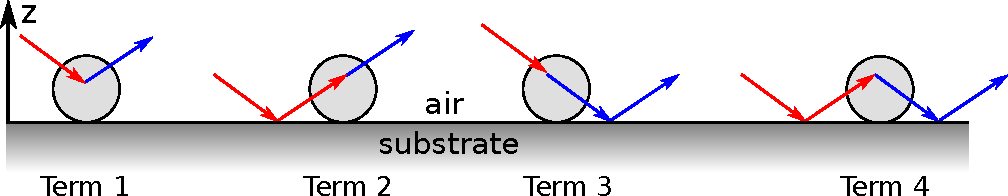
\includegraphics[width=\textwidth]{fig/drawing/drawingDWBA.pdf}
\end{center}
\caption{Schematic views of the different terms appearing in the expression of the form factor under DWBA for particles sitting on a substrate layer.}
\label{fig:SchemDWBA}
\end{figure}


Script~\ref{lst:badwba} illustrates the difference between BA and DWBA in \BornAgain\ when generating the sample.  We consider the simple case of:
\begin{itemize}
\item one kind of particles' shape,
\item no interference between the particles,
\item in the DWBA, a sample made of a layer of substrate on which are deposited the particles,
\item in the BA, a sample composed of the particles in air.
\end{itemize} 

Figure~\ref{fig:spheroidbadwba} shows the intensity contour plot generated using this script with truncated spheroids as particles.

\newpage

\begin{lstlisting}[language=python, style=eclipseboxed,numbers=none,nolol,caption={\Code{Python} script to generate a sample using Born (BA) or distorted-wave Born approximation (DWBA). The difference between BA and DWBA in this simple case is the absence or presence of a substrate layer in the sample.},label={lst:badwba}]
def get_sample():
    """
    Build and return the sample to calculate form factor of 
    truncated spheroid in Born or distorted-wave Born Approximation.
    """
    # defining materials
    m_ambience = HomogeneousMaterial("Air", 0.0, 0.0)
    m_substrate = HomogeneousMaterial("Substrate", 6e-6, 2e-8)
    m_particle = HomogeneousMaterial("Particle", 6e-4, 2e-8)

    # collection of particles
    ff= FormFactorTruncatedSpheroid(7.5*nanometer, 9.0*nanometer, 1.2)
    particleshape = Particle(m_particle, ff)
    particle_layout = ParticleLayout()
    particle_layout.addParticle(particleshape, 0.0, 1.0)

    # interferences
    interference = InterferenceFunctionNone()
    particle_layout.addInterferenceFunction(interference)

    # assembling the sample
    air_layer = Layer(m_ambience)
    air_layer.addLayout(particle_layout)
    substrate_layer = Layer(m_substrate, 0)

    multi_layer = MultiLayer()
    multi_layer.addLayer(air_layer)
    # Comment the following line out for Born Approximation
    multi_layer.addLayer(substrate_layer)
    return multi_layer
\end{lstlisting}


\begin{figure}[ht]
\hfill
\subfigure[Born Approximation]{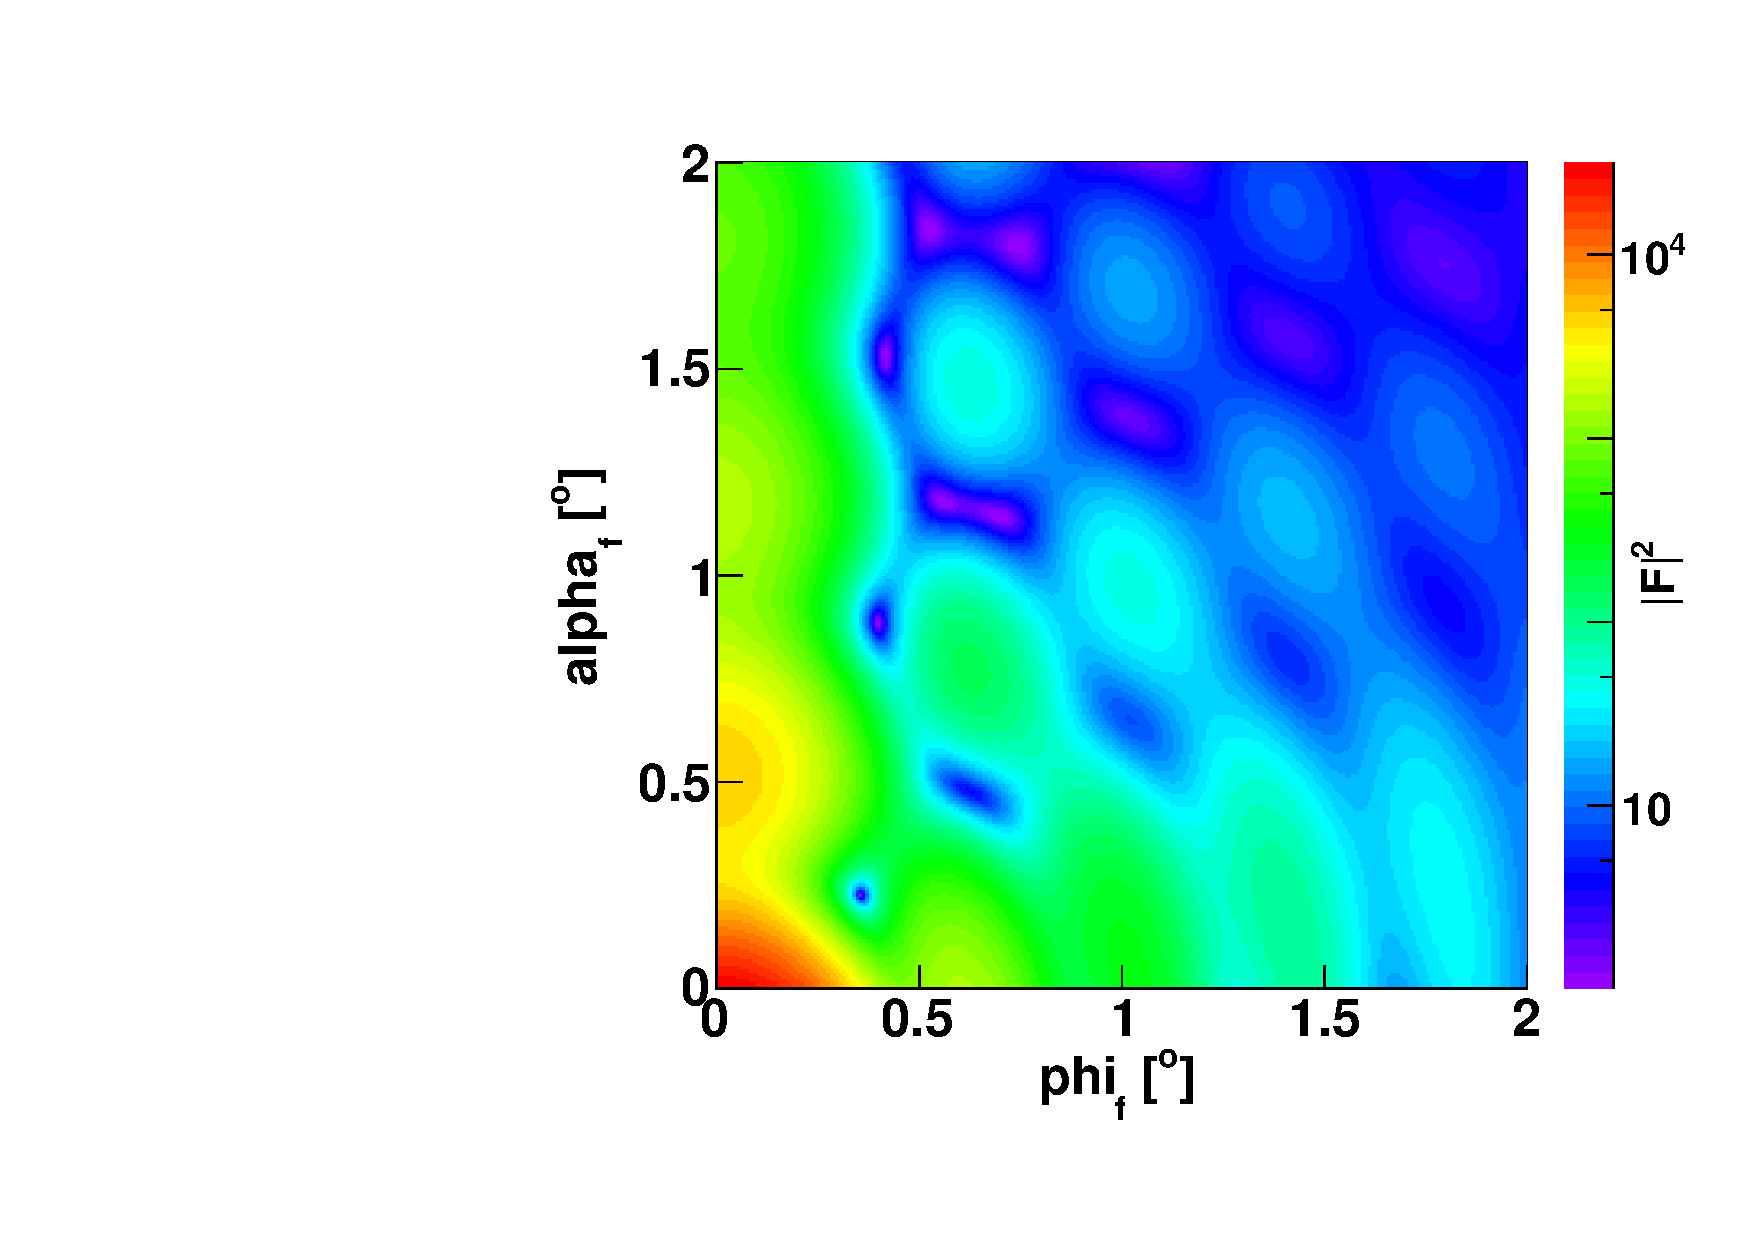
\includegraphics[angle=-90,width=6cm]{fig/gisasmap/ffspheroidBA.pdf}}
\hfill
\subfigure[DWB Approximation]{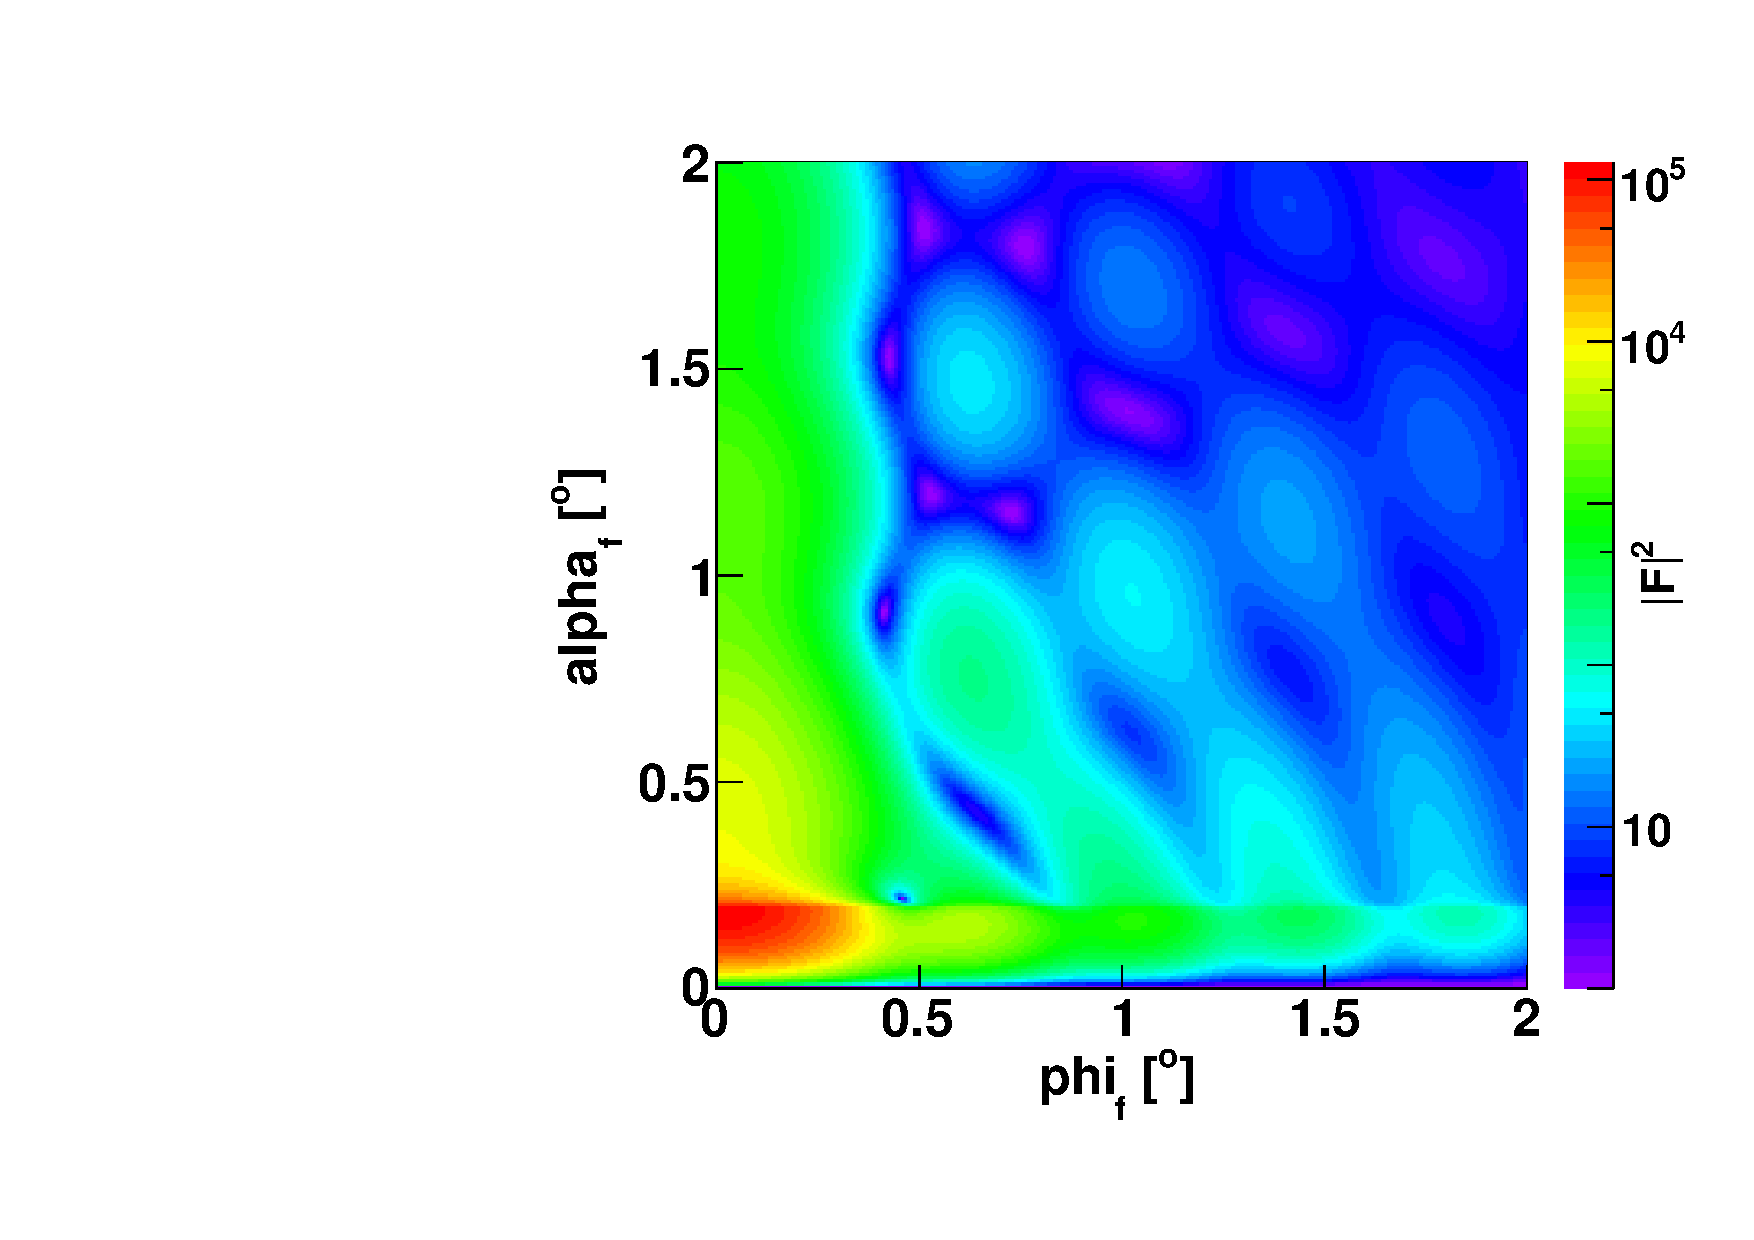
\includegraphics[angle=-90,width=6cm]{fig/gisasmap/ffspheroidDWBA.pdf}}
\hfill
\caption{Intensity map of TruncatedSpheroid form factor in BA and DWBA computing using script~\ref{lst:badwba} for the sample.}
\label{fig:spheroidbadwba}
\end{figure}

\FloatBarrier 

\ImportantPoint{Remark:}{In \BornAgain, the DWBA is implemented automatically when assembling the sample with more layers than only the air layer (for example, for particles are sitting on a substrate).}

%-------------------------------------------------------------------------------
\subsection{Buried particles} 
%-------------------------------------------------------------------------------

The system considered in this section consists of particles encapsulated in a layer, which is sitting on a substrate (see fig.~\ref{fig:SchemDWBAburied}). In this case the form factor in the DWBA is given by

\begin{align}
  F_{\rm{DWBA}}(q_{\parallel}, k_{i,z}, k_{f,z})
  &= T_\text{i} T_\text{f} F_{\rm{BA}}(q_{\parallel}, k_{i,z}-k_{f,z})e^{i(k_{i,z}-k_{f,z})d}\nonumber \\
  &+ R_\text{i} T_\text{f} F_{\rm{BA}}(q_{\parallel}, -k_{i,z}-k_{f,z})e^{i(-k_{i,z}-k_{f,z})d} \nonumber \\
  &+ R_\text{f} T_\text{i} F_{\rm{BA}}(q_{\parallel}, k_{i,z}+k_{f,z}) e^{i(k_{i,z}+k_{f,z})d}\nonumber \\
  &+ R_\text{f} R_\text{i}F_{\rm{BA}}(q_{\parallel},-k_{i,z}+k_{f,z})e^{i(-k_{i,z}+k_{f,z})d}, \label{Edwbaburied}
\end{align}

\begin{equation*}
R_j =\frac{t^{j}_{0,1}r^{j}_{1,2}\exp(2ik_{j,z}t)}{1+r^{j}_{0,1}r^{j}_{1,2}\exp(2ik_{j,z}t)}, \quad T_j=\frac{t^{j}_{0,1}}{1+r^{j}_{0,1}r^{j}_{1,2}\exp(2ik_{j,z}t)}, j=i,f 
\end{equation*}
where $q_{\parallel}$ is the component of the scattering beam in the plane of the interface, $k_{i,z}$ and $k_{f,z}$ are the z-component of the incident and scattered beams, respectively.  $d$ is the depth at which the particles are sitting in the layer. Note that this value is given relative to the top of this layer and it is not the coordinate in the absolute referential (linked with the full sample) and it is measured up to the bottom of the particle. $t$ is the thickness of the intermediate layer containing the particles. $R_{i,f}$ and $T_{i,f}$  are the reflection  and transmission coefficients in incidence and reflection (they can be calculated using Parratt or matrix formalism). $r^j_{0,1}$, $r^j_{1,2}$ $t^j_{0,1}$ are the reflection and transmission coefficients between layers; the indices are related to different boundaries with 0: air, 1: intermediate layer and 2: substrate layer and the superscript $j$ is associated with the incident or scattered beams:
\begin{equation*}
r^j_{n,n+1}=\frac{k_{j,z,n}-k_{j,z,n+1}}{k_{j,z,n}-k_{j,z,n+1}}, \qquad t^j_{n,n+1}= \frac{2k_{j,z,n}}{k_{j,z,n}-k_{j,z,n+1}}, \quad n=0,1, \quad j=i,f,
\end{equation*}
where index $n$ is related to the layers, $z$ to the vertical component, and $j$ to the beams (incident and outgoing).

\begin{figure}[ht]
\begin{center}
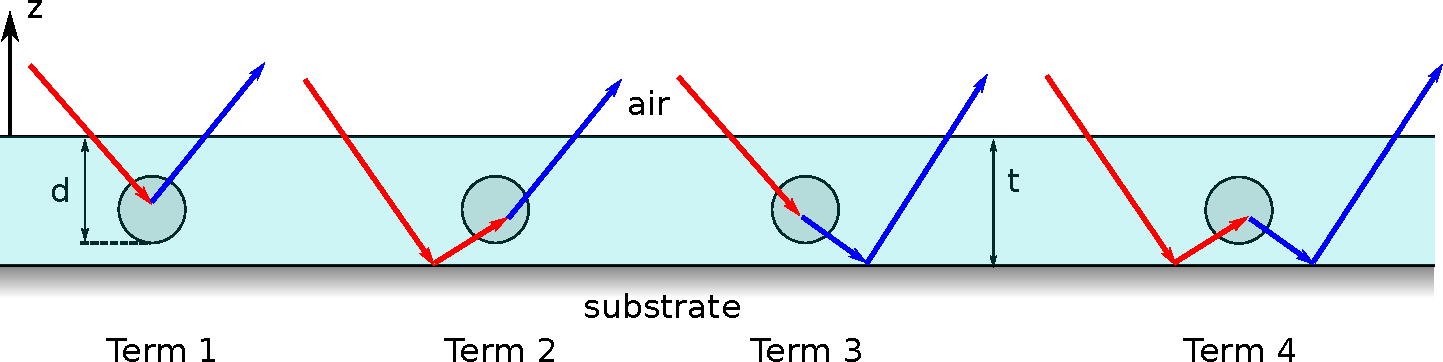
\includegraphics[width=\textwidth]{fig/drawing/drawingDWBAburied.pdf}
\end{center}
\caption{Schematic views of the different terms appearing in the expression of the form factor under the DWBA for buried particles.}
\label{fig:SchemDWBAburied}
\end{figure}


Figure~\ref{fig:dwbaburied} shows a typical example of the output intensity scattered from a sample made of 3 layers: air, substrate, and in between, spherical particles embedded in the middle of a 30~nm-thick layer. This figure had been generated using listing~\ref{lst:dwbaburied}.

\begin{lstlisting}[language=python, style=eclipseboxed,numbers=none,nolol,caption={\Code{Python} script to generate a sample where spherical particles are embedded in the middle of a layer on a substrate.},label={lst:dwbaburied}]
def get_sample():
    """
    Build and return the sample with buried spheres in DWBA.
    """
    # defining materials
    m_ambience = HomogeneousMaterial("Air", 0.0, 0.0)
    m_interm_layer = HomogeneousMaterial("IntermLayer",3.45e-6, 5.24e-9)
    m_substrate = HomogeneousMaterial("Substrate", 7.43e-6, 1.72e-7)
    m_particle = HomogeneousMaterial("Particle", 0.0, 0.0)

    # collection of particles 
    ff = FormFactorFullSphere(10.2*nanometer)
    particleshape = Particle(m_particle, ff)
    particle_layout = ParticleLayout()
    particle_layout.addParticle(particleshape,25.2,1.0)

    # interferences 
    interference = InterferenceFunctionNone()
    particle_layout.addInterferenceFunction(interference)

    # assembling the sample 
    air_layer = Layer(m_ambience)
    intermediate_layer = Layer(m_interm_layer, 30.*nanometer)
    intermediate_layer.addLayout(particle_layout)
    substrate_layer = Layer(m_substrate, 0)
   
    multi_layer = MultiLayer()
    multi_layer.addLayer(air_layer)
    multi_layer.addLayer(intermediate_layer)
    multi_layer.addLayer(substrate_layer)
    return multi_layer
\end{lstlisting}


\begin{figure}[ht]
\centering
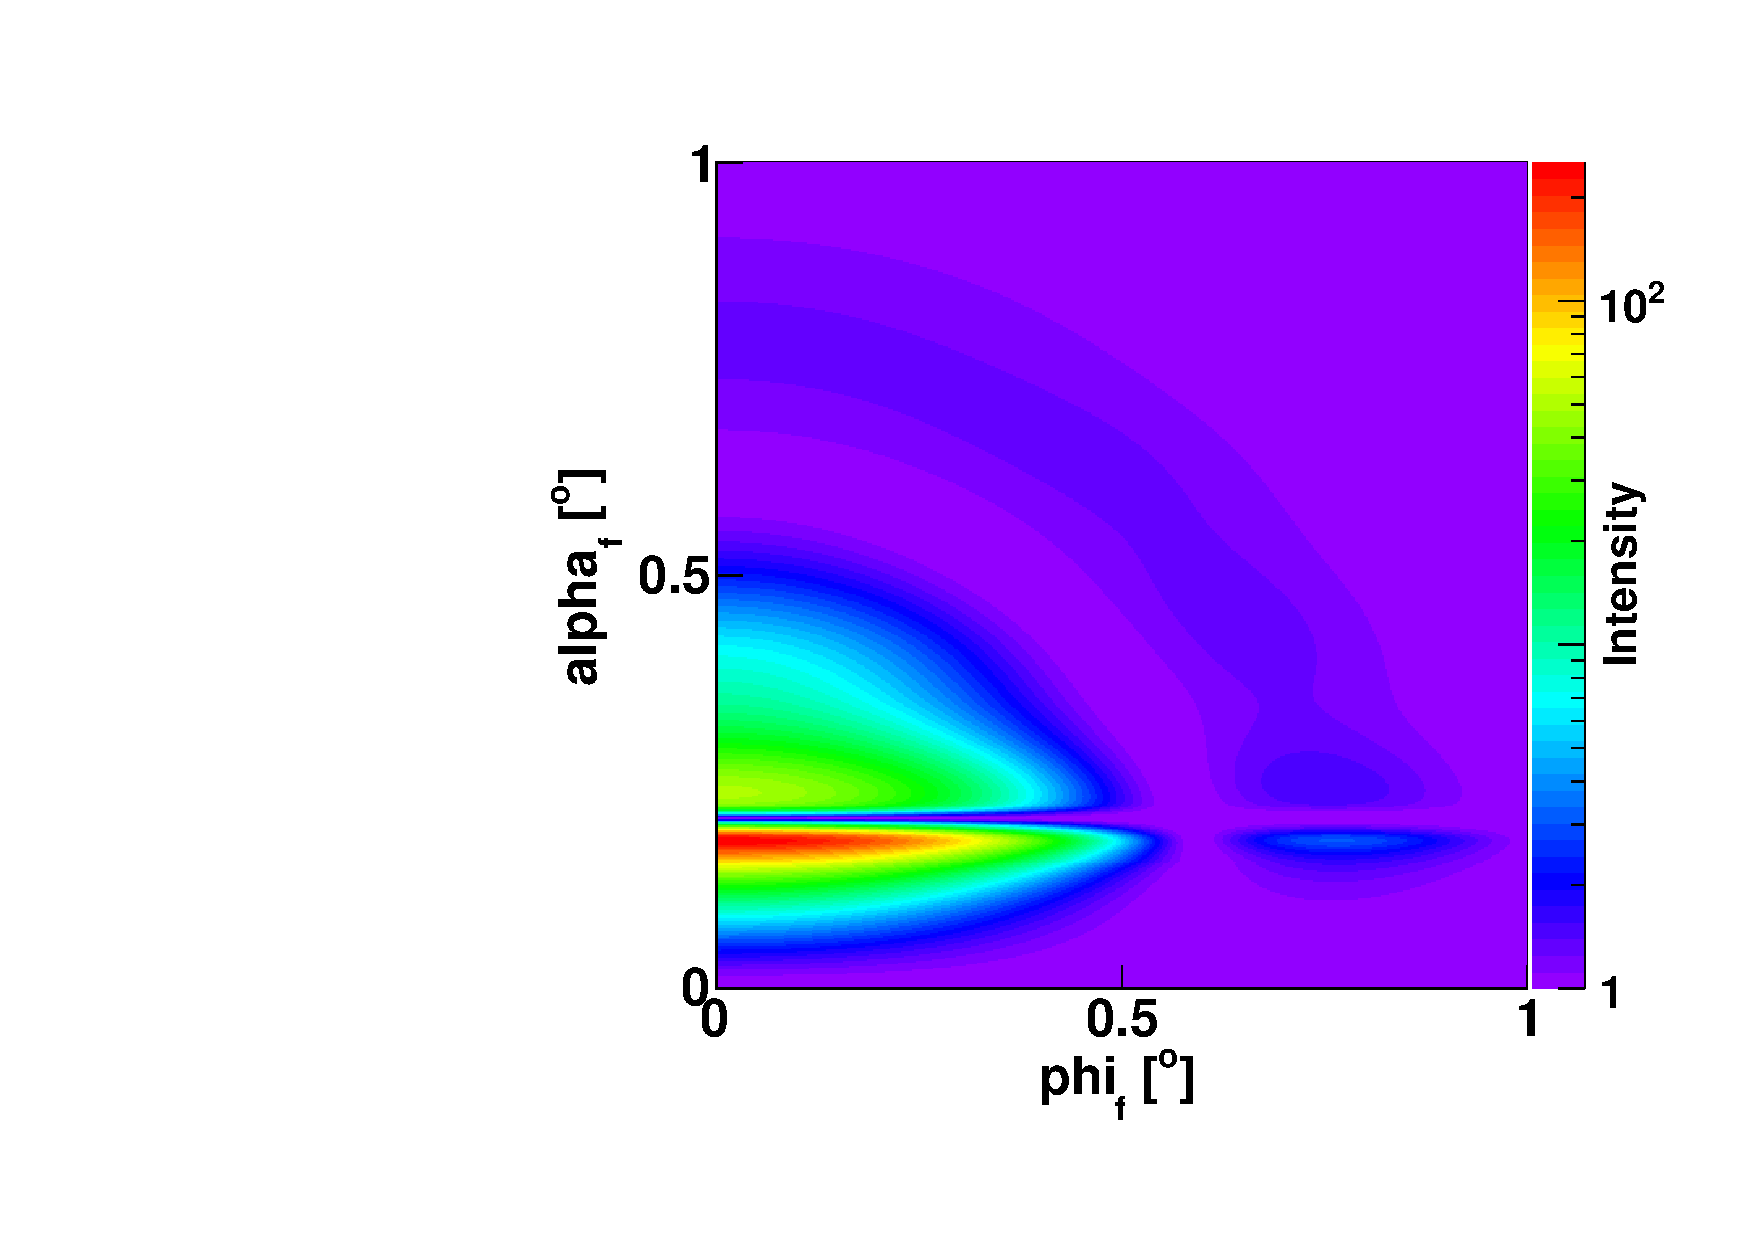
\includegraphics[angle=-90,width=0.6\textwidth]{fig/gisasmap/figIntBuriedPart.pdf}
\caption{Map of intensity scattered from a sample made of spherical particles embedded in the middle of a 30~nm-thick layer on a substrate (see Script~\ref{lst:dwbaburied} for details about the sample).}
\label{fig:dwbaburied}
\end{figure}

\newpage

\ImportantPoint{Remark:}{For layers different from the air layer, the top interface is considered as the reference level to position the encapsulated particles. For example, spheres positioned at depth $d$ (positive) are located at a distance $d$ from the top of the layer up to the bottom of these particles. This convention is different for the top air layer, where particles sitting at the interface with an underlying layer (\textit{i.e.} the bottom of the air layer) are located at depth 0 (see fig.~\ref{fig:depthpartBA}).}


\begin{figure}[ht]
\centering
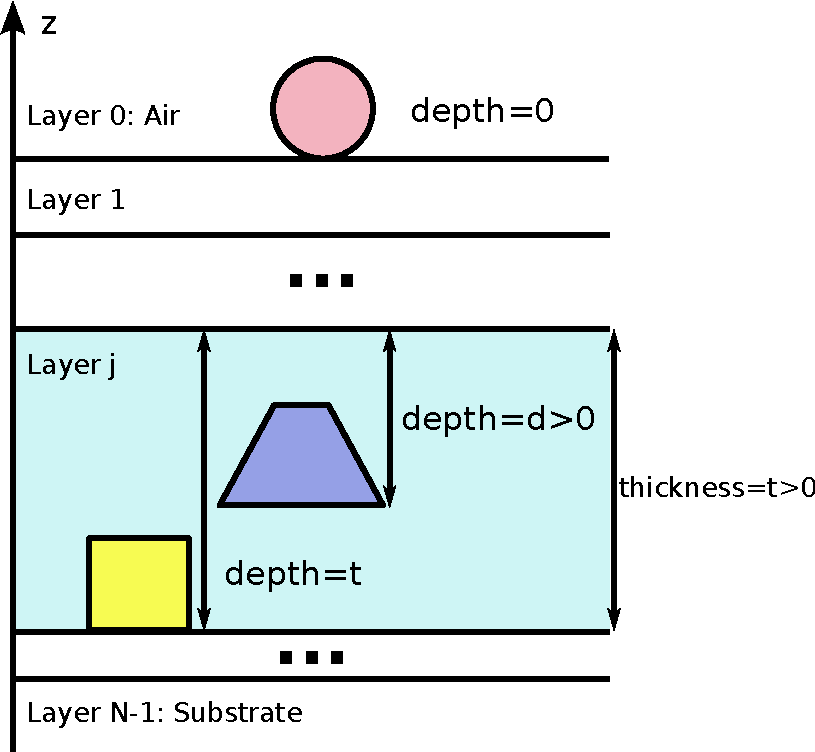
\includegraphics[width=0.5\textwidth]{fig/drawing/drawingDepthParticle.pdf}
\caption{Illustration of the convention about \Code{depth} used in \BornAgain\ to encapsulate particles in layers.}
\label{fig:depthpartBA}
\end{figure}



%===============================================================================
\subsection{Implementation in \BornAgain}
%===============================================================================

This section describes the implementation of the interference functions in \BornAgain. For an implementation of all the components of a simulation, the use is referred, for example, to Sect.~\ref{sec:Example1Python}.\\


\ImportantPoint{Remark:}{In \BornAgain\ the particles are positioned in the same vertical layer.}

\subsubsection{Size-distribution models}
\index{Size-distribution models}
The decoupling approximation (DA), local monodisperse approximation (LMA) and size spacing correlation approximation (SSCA) can be used in \BornAgain.
The selection between DA and SSCA is made using\\ 
\Code{ILayout.setApproximation(EInterferenceFunction approximation)} when defining the characteristics of the way particles and interference functions are embedded in a layer.  For example,
\begin{lstlisting}[language=python, style=eclipseboxed,numbers=none,nolol]
    particle_layout = ParticleLayout()
   ....
# interference approx chosen between: DA (default) and SSCA
    particle_layout.setApproximation(ILayout.DA)
\end{lstlisting}

Note that with the SSCA, the users have to specify the coupling parameter $\kappa$ (with the function \Code{setKappa}), which should be a positive dimensionless value. $\kappa$ characterizes the influence of the neighboring particles' sizes on their distance. If $\kappa=0$, the SSCA reduces to the DA with a radial paracrystal for the interference function.\\

For the LMA, its implementation is automatically done when using more than one layout of particles:
\begin{lstlisting}[language=python, style=eclipseboxed,numbers=none,nolol]
    particle_layout0 = ParticleLayout()
    particle_layout1 = ParticleLayout()
   ....
# association of each particles' layout with materials, form factors
#... and with a material layer
    layer_a = Layer(m_material_a)
    layer_a.addLayout(particle_layout0)
    layer_a.addLayout(particle_layout1)
\end{lstlisting}

%%ADD EXPLANATION ABOUT LMA

%-------------------------------------------------------------------------------
\subsubsection{Probability distribution functions}\label{baftd}
%-------------------------------------------------------------------------------

The probability distribution functions have been implemented in the reciprocal space in \BornAgain. Their expressions are given in Table~\ref{table:pdf}.

\begin{table}[H]
\centering
\begin{tabular}{ccc}
\hline 
Function & One dimension & Two dimensions\\
\hline 
Cauchy & $(1+q^2\omega^2)^{-3/2}$ & $(1 + q_x^2 cl_x^2 + q_y^2 cl_y^2)^{-3/2}$ \\
Gauss & $\dfrac{1}{2}\exp(-\dfrac{q^2\omega^2}{4})$ & $\frac{1}{2}\exp\left(-\dfrac{q_x^2 cl_x^2+ q_y^2cl_y^2}{4}\right)$ \\
Voigt & $\dfrac{\eta}{2} \exp\left(-\dfrac{q^2\omega^2}{4}\right) + \dfrac{1 - \eta}{(1 + q^2\omega^2)^{3/2}}$ & $\dfrac{\eta}{2} \exp\left(-\dfrac{q_x^2 cl_x^2+ q_y^2cl_y^2}{4}\right)+ \dfrac{1 - \eta}{(1 + q_x^2 cl_x^2+ q_y^2cl_y^2)^{3/2}}$ \\
\hline
\end{tabular}
\caption{List of probability distribution functions in reciprocal space. $\omega$, $cl$ stand for coherence lengths (the index refers to the axis) and  $\eta$ is a weighting coefficient.}
\label{table:pdf}
\end{table}

The Cauchy distribution corresponds to $\exp(-r)$ in real space and the Voigt one  is a linear combination of the Gaussian and Cauchy probability distribution functions.\\

\noindent \underline{One dimension}
\begin{itemize}
\item \Code{FTDistribution1DCauchy($\omega$)},
\item \Code{FTDistribution1DGauss($\omega$)},
\item \Code{FTDistribution1DVoigt($\omega, \eta$)}.
\end{itemize}
where $\omega$ is the coherence length and $\eta$ is a weighting factor.\\

\noindent \underline{Two dimensions}
\begin{itemize}
\item \Code{FTDistribution2DCauchy($cl_x$, $cl_y$)},
\item \Code{FTDistribution2DGauss($cl_x$, $cl_y$)},
\item \Code{FTDistribution2DVoigt($cl_x$, $cl_y$)}
\end{itemize}
where $cl_{x,y}$ are the coherence lengths in the $x$ or $y$ direction, respectively.

These functions can be used with all interference functions, except the case without any interference.

%-------------------------------------------------------------------------------
\subsubsection{Interferences}
%-------------------------------------------------------------------------------
\index{Interference function}

The interference function is specified when building the sample. It is linked with the particles (shape, material). Examples of implementation are given at the end of each description.

\paragraph{Syntax:}
 \Code{particle\_layout.addInterferenceFunction(interference\_function)},\\ where \Code{particle\_layout} holds the information about the different shapes and their proportions for a given layer of particles, and \Code{interference\_function}  is one of the following expressions:
\begin{itemize}
\item \Code{InterferenceFunctionNone()}
\item \Code{InterferenceFunction1DLattice(lattice\_parameters)}
\item \Code{InterferenceFunctionRadialParaCrystal(peak\_distance, damping\_length)}
\item \Code{InterferenceFunction2DLattice(lattice\_parameters)}
\item \Code{InterferenceFunction2DParaCrystal(length\_1, length\_2, $\alpha$\_lattice, $\xi$, \\ damping\_length)}
\end{itemize}

\ImportantPoint{Remark:}{\Code{InterferenceFunction1DLattice} can only be used for particles which are infinitely long in one direction of the sample's surface like for example a rectangular grating.}

\newpage
%-------------------------------------------------------------------------------
\subsubsection{\Code{InterferenceFunctionNone()}} 
%-------------------------------------------------------------------------------

The particles are placed randomly in the dilute limit and are considered as individual, non-interacting scatterers. The scattered intensity is function of the form factors only. 

\paragraph{Example} The sample is made of a substrate on which are deposited half-spheres. Script~\ref{lst:nointerf} details the commands necessary to generate such a sample. Figure~\ref{fig:nointerf} shows an example of output intensity: Script~\ref{lst:nointerf}  + detector's + input beam's characterizations.


\begin{figure}[ht]
\begin{center}
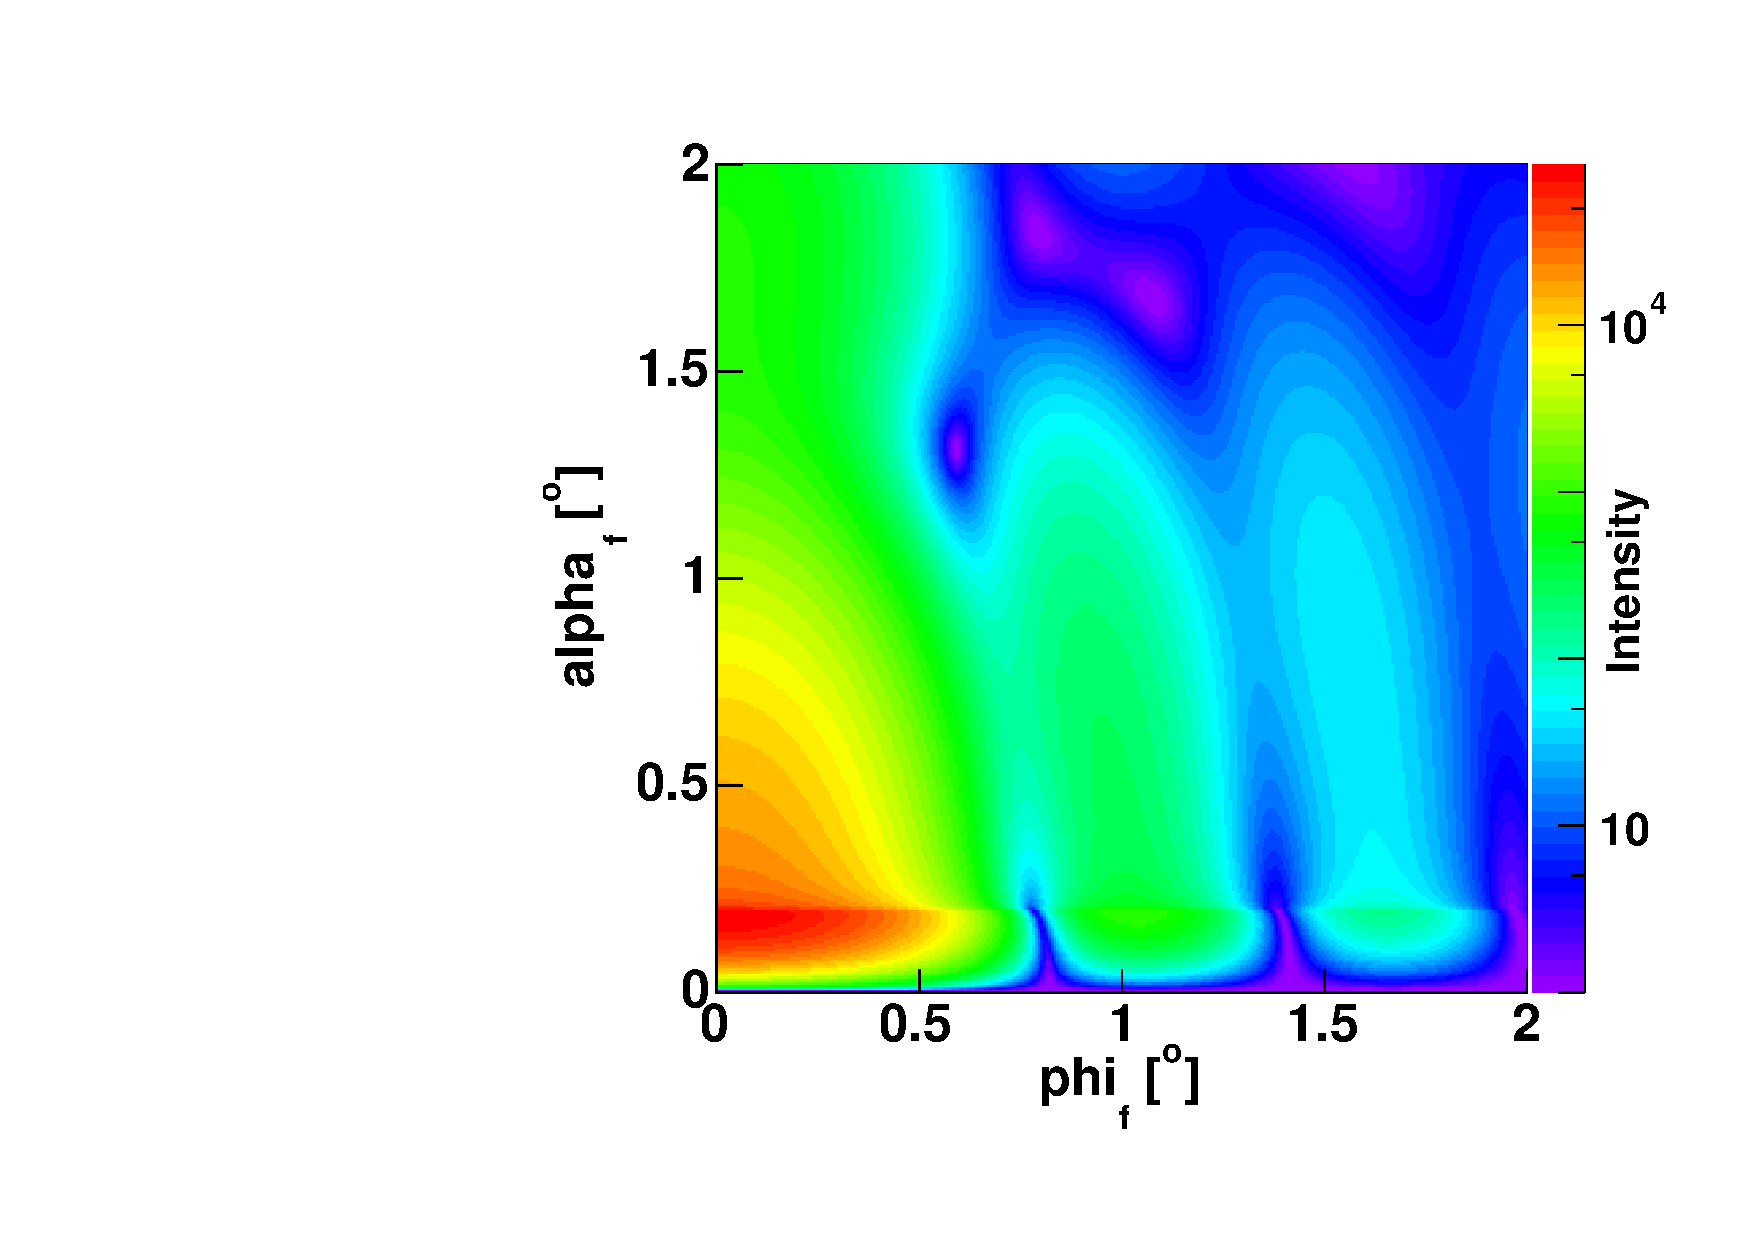
\includegraphics[angle=-90,width=0.5\textwidth]{fig/gisasmap/HSphere_NoInterf.pdf}
\end{center}
\caption{Output intensity scattered from a sample made of half-spheres with no interference between them.}
\label{fig:nointerf}
\end{figure}

\FloatBarrier
\newpage

\begin{lstlisting}[language=python, style=eclipseboxed,numbers=none,nolol,caption={\Code{Python} script to simulate a sample made of half-spheres deposited on a substrate layer without any interference. The part specific to the interferences is marked in a red italic font.},label={lst:nointerf}]
def get_sample():
    """
    Build and return the sample representing particles with no interference
    """
    # defining materials
    m_ambience = HomogeneousMaterial("Air", 0.0, 0.0)
    m_substrate = HomogeneousMaterial("Substrate", 6e-6, 2e-8)
    m_particle = HomogeneousMaterial("Particle", 6e-4, 2e-8)
    # collection of particles
    sphere_ff = FormFactorTruncatedSphere(5*nanometer, 5*nanometer)
    sphere = Particle(m_particle, sphere_ff)
    particle_layout = ParticleLayout()
    particle_layout.addParticle(sphere, 0.0, 1.0)
    |interference = InterferenceFunctionNone()| 
    |particle_layout.addInterferenceFunction(interference)|
    # assembling the sample
    air_layer = Layer(m_ambience)
    air_layer.addLayout(particle_layout)
    substrate_layer = Layer(m_substrate, 0)

    multi_layer = MultiLayer()
    multi_layer.addLayer(air_layer)
    multi_layer.addLayer(substrate_layer)
    return multi_layer
\end{lstlisting}

\newpage
%-------------------------------------------------------------------------------
\subsubsection{\Code{InterferenceFunction1DLattice(lattice\_length, xi)}} 
%-------------------------------------------------------------------------------
where lattice\_length is the lattice constant and $\xi$ the angle in radian between the lattice unit vector and the $\mathbf{x}$-axis of the reference Cartesian frame as shown in fig.~\ref{fig:1dgrating}.

\begin{figure}[ht]
\begin{center}
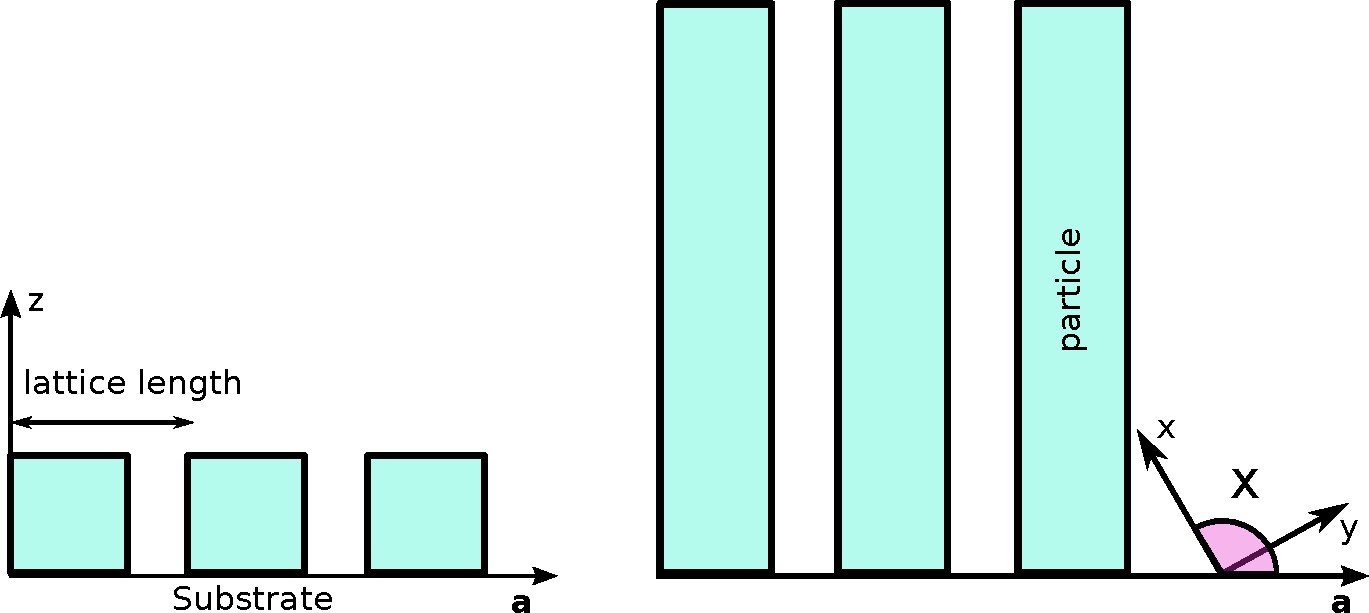
\includegraphics[width=0.75\textwidth]{fig/drawing/1DGrating.pdf}
\end{center}
\caption{Schematic representation of a 1D lattice (side and top views). Such a lattice is characterized by a lattice length and the angle $\xi$.}
\label{fig:1dgrating}
\end{figure}

\ImportantPoint{Remark:}{By default the long axis of the particles in this 1D lattice is along the beam axis. That is the reason why in the example below the particles are rotated by  $90^{\circ}$ in the $(x,y)$ plane: the main axis of the lattice is therefore parallel to the y-axis, perpendicular to the long axis of the particles.}

\vspace{12pt}
A probability distribution function \Code{pdf} has to be chosen from the list in section~\ref{baftd} in order to apply some modifications to the scattering peaks. This function is implemented using \Code{setProbabilityDistribution(pdf)}. 

\paragraph{Example:} Script~\ref{lst:1dlattinterf} details how to build in  \BornAgain\ a sample using\\ \Code{InterferenceFunction1DLattice} as the interference function. As mentioned previously, this interference function can only be used with infinitely wide or long particles.\\ Here the sample is made of infinitely long boxes deposited on a substrate (these particles are characterized by their widths and heights). They are also rotated by $90^{\circ}$  in the sample surface in order to have their long axis perpendicular to the input beam, which is along the $x$-axis.\\
 The lattice parameters (the lattice length and angle between the lattice main axis and the $x$-axis) are passed into the constructor of the interference function.

\newpage
\begin{lstlisting}[language=python, style=eclipseboxed,numbers=none,nolol,caption={\Code{Python} script to generate a sample made of infinitely long boxes deposited on a substrate layer with the 1DLatticeInterference function. The part specific to the interferences is marked in a red italic font.},label={lst:1dlattinterf}]
def get_sample():
    """
    Build and return the sample with 1DLatticeInterference function
    """
    # defining materials
    m_air = HomogeneousMaterial("Air", 0.0, 0.0)
    m_substrate = HomogeneousMaterial("Substrate", 6e-6, 2e-8)
    m_particle = HomogeneousMaterial("Particle", 6e-4, 2e-8)

    # collection of particles
    ff = FormFactorInfLongBox(10.*nanometer, 15.0*nanometer)
    box = Particle(m_particle, ff)
    particle_layout = ParticleLayout()
    transform = Transform3D.createRotateZ(90.0*degree)
    particle_layout.addParticle(box, transform)

    # interference function
    |interference = InterferenceFunction1DLattice(30.0*nanometer, 0.0*degree)|
    |pdf = FTDistribution1DCauchy(200./2./M_PI*nanometer)|
    |interference.setProbabilityDistribution(pdf)|
    |particle_layout.addInterferenceFunction(interference)|

    # air layer with particles and substrate form multi layer
    air_layer = Layer(m_air)
    air_layer.addLayout(particle_layout)
    substrate_layer = Layer(m_substrate, 0)

    multi_layer = MultiLayer()
    multi_layer.addLayer(air_layer)
    multi_layer.addLayer(substrate_layer)
    return multi_layer
\end{lstlisting} 

\newpage
%-------------------------------------------------------------------------------
\subsubsection{\Code{InterferenceFunctionRadialParaCrystal(peak\_distance, damping\_length)}}  
%-------------------------------------------------------------------------------
\begin{itemize}
\item[where] \Code{peak\_distance} is the average distance to the first neighbor peak, 
\item[]\Code{width} is the width parameter of the probability distribution,
\item[] \Code{damping\_length} is used to introduce finite size effects by applying a multiplicative coefficient equal to  $\exp$(-\Code{peak\_distance/damping\_length}) to the Fourier transform of the probability densities. \Code{damping\_length} is equal to 0 by default and, in this case, no correction is applied.
\end{itemize}

A probability distribution function \Code{pdf} has to be chosen from the list in section~\ref{baftd} in order to apply some modifications to the scattering peaks. This function is implemented using \Code{setProbabilityDistribution(pdf)}. 


\MakeRemark{Remark}{
This interference function is not one-dimensional.  It takes into account the radial component of the scattering vector.
}

\paragraph{Example}
To illustrate the radial paracrystal interference function, we use the same sample as in the case without interference: half-spheres deposited on a substrate.

\begin{lstlisting}[language=python, style=eclipseboxed,numbers=none,nolol,caption={\Code{Python} script to define the radial paracrystal interference function between half-spheres, where \Code{trsphere} is of type \Code{Particle}.},label={lst:1dpara}]
    particle_layout = ParticleLayout()
    particle_layout.addParticle(trsphere, 0.0, 1.0)
    interference = InterferenceFunctionRadialParaCrystal(25.0*nanometer, 1e3*nanometer)
    pdf = FTDistribution1DGauss(7 * nanometer)
    interference.setProbabilityDistribution(pdf)
    particle_layout.addInterferenceFunction(interference)
\end{lstlisting}



\begin{figure}[ht]
\begin{center}
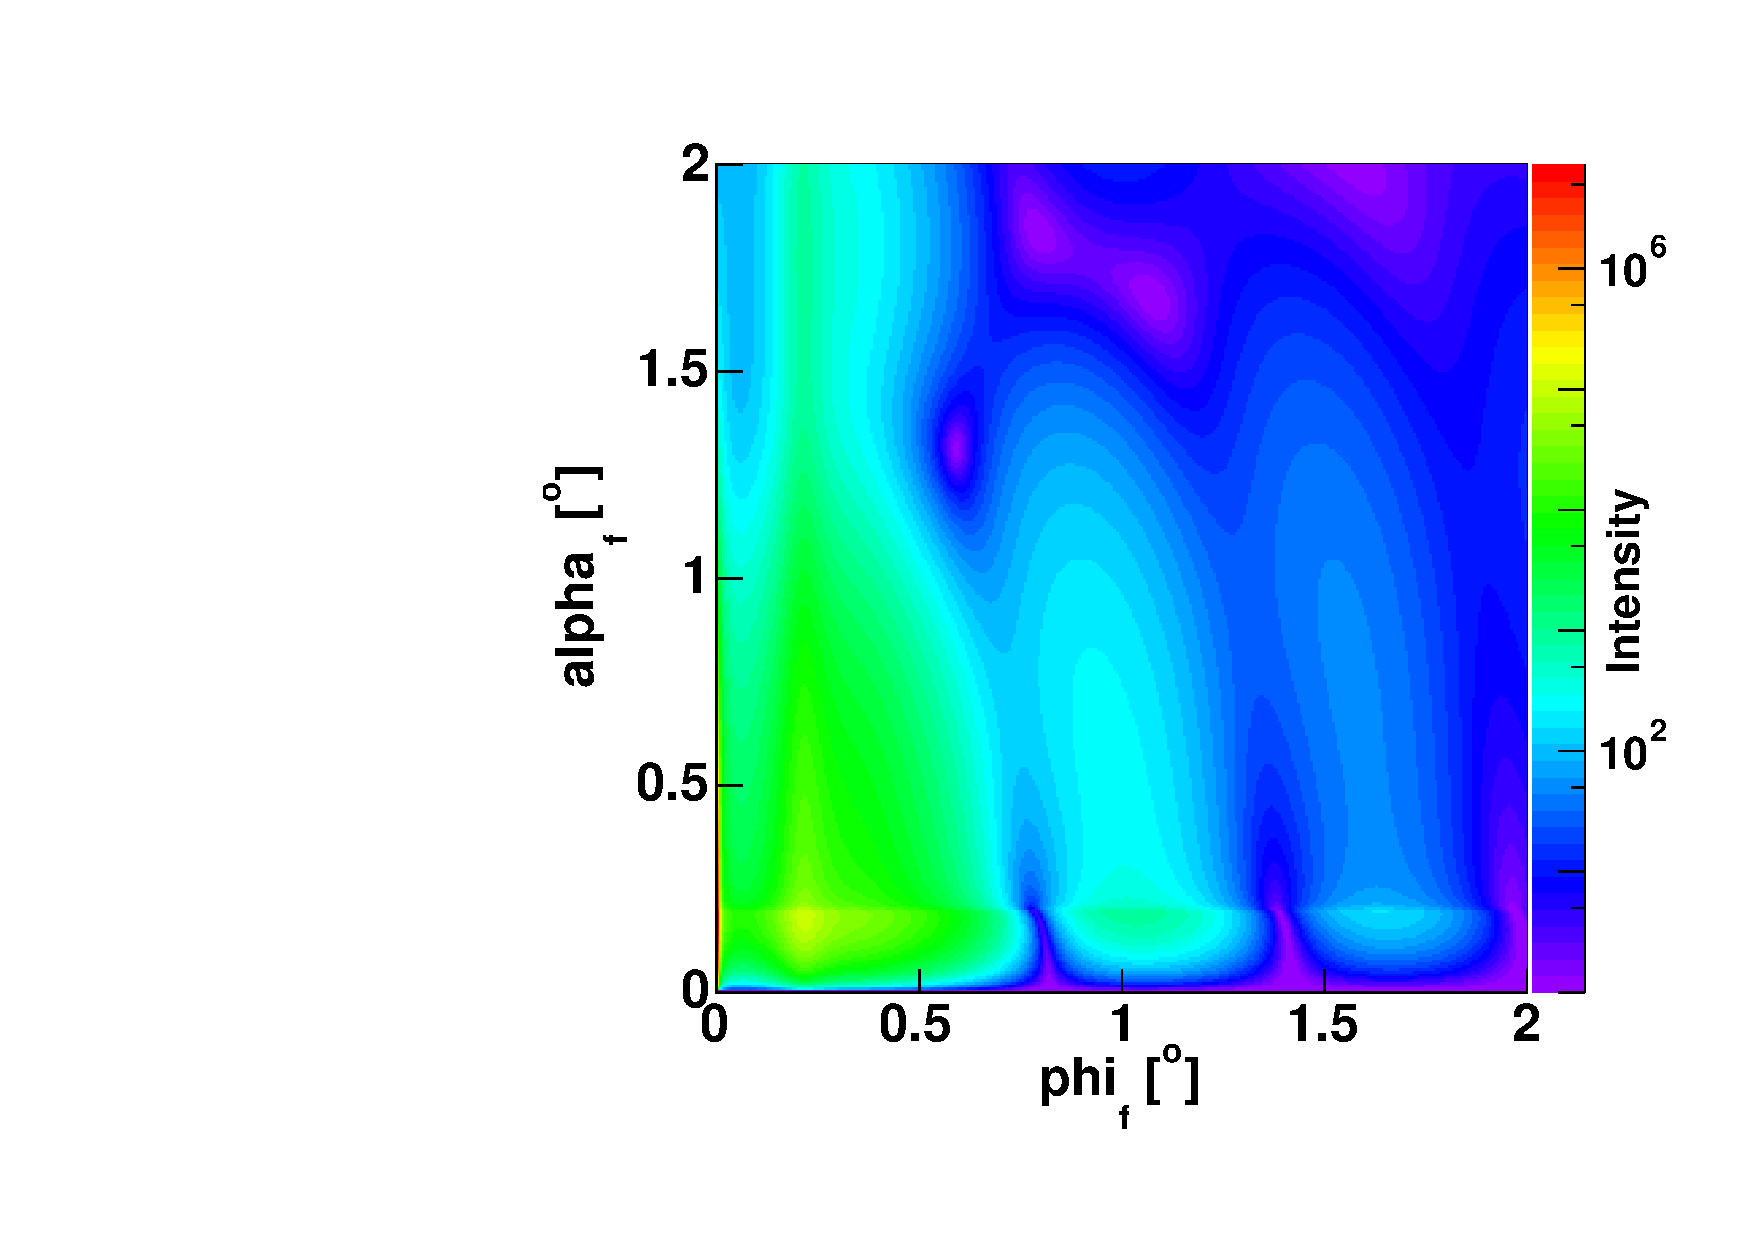
\includegraphics[angle=-90,width=0.5\textwidth]{fig/gisasmap/HSphere_1DDL.pdf}
\end{center}
\caption{Output intensity scattered from a sample made of half-spheres with the radial paracrystal interference between them. This figure has been generated using Script~\ref{lst:1dpara} for the interference function.}
\label{fig:1ddl}
\end{figure}

\FloatBarrier

\newpage
%-------------------------------------------------------------------------------
\subsubsection{\Code{InterferenceFunction2DLattice(L\_1, L\_2, alpha, xi)}} 
%-------------------------------------------------------------------------------
where ($L_1$, $L_2$, $\alpha$, $\xi$) are shown in figure~\ref{fig:2dlattice} with 
\begin{itemize}
\item[]$L_1$, $L_2$ the lengths of the lattice cell, 
\item[]$\alpha$ the angle between the lattice basis vectors $\mathbf{a}, \mathbf{b}$ in direct space,
\item[] $\xi$ is the angle defining the lattice orientation (set to $0$ by default); it is taken as the angle between the $\mathbf{a}$ vector of the lattice basis and the $\mathbf{x}$ axis of the reference Cartesian frame (as shown in figure~\ref{fig:multil3d}).
\end{itemize}

\begin{figure}[ht]
\begin{center}
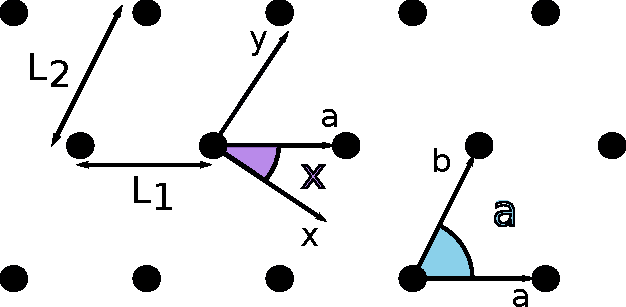
\includegraphics[width=0.5\textwidth]{fig/drawing/2Dlattice.pdf}
\end{center}
\caption{Schematic representation of a 2D lattice (top view). Such a lattice is characterized by lattice lengths $L_1$, $L_2$ and angles $\alpha$ and $\xi$.}
\label{fig:2dlattice}
\end{figure}

Like for the one-dimensional case, a probability distribution function \Code{pdf} has to be defined. One can choose between those listed in Section~\ref{baftd} and implements it using \Code{setProbabilityDistribution(pdf)}.

\paragraph{Example} The sample used to run the simulation is made of half-spheres deposited on a substrate. The interference function is "2Dlattice" and the particles are located at the nodes of a square lattice with $L_1=L_2=20$~nm, $\mathbf{a}\equiv \mathbf{b}$ and the probability distribution function is Gaussian. We also use the Decoupling Approximation. 

\begin{lstlisting}[language=python, style=eclipseboxed,numbers=none,nolol,caption={\Code{Python} script to define a 2DLattice interference function between hemi-spherical particles as well as the Decoupling Approximation in \Code{getSimulation()}.  The part specific to the interferences is marked in a red italic font.},label={lst:2dlatticeinterf}]
    #collection of particles
    sphere_ff = FormFactorTruncatedSphere(5*nanometer, 5*nanometer)
    sphere = Particle(m_particle, sphere_ff)
    |interference = InterferenceFunction2DLattice(20.0*nanometer, 20.0*nanometer, 90.0*degree, 0.0*degree)|
    |pdf = FTDistribution2DGauss(200.0*nanometer/2.0/M_PI, 75.0*nanometer/2.0/M_PI)|
    |interference.setProbabilityDistribution(pdf)|
    particle_layout = ParticleLayout()
    particle_layout.addParticle(sphere, 0.0, 1.0)
    |particle_layout.addInterferenceFunction(interference)|

    # interference approx chosen between: DA (default) and SSCA
    |particle_layout.setApproximation(ILayout.DA)|
\end{lstlisting}
 
%\begin{lstlisting}[language=python, style=eclipseboxed,numbers=none,nolol]
%def get_simulation():
%    """
%    Create and return GISAXS simulation with beam and detector
%    """
%    simulation = Simulation()
%    simulation.setDetectorParameters(100, 0.0*degree, 2.0*degree, 100, 0.0*degree, 2.0*degree, True)
%    simulation.setBeamParameters(1.0*angstrom, 0.2*degree, 0.0*degree)
%    return simulation
%\end{lstlisting}


\begin{figure}[ht]
\begin{center}
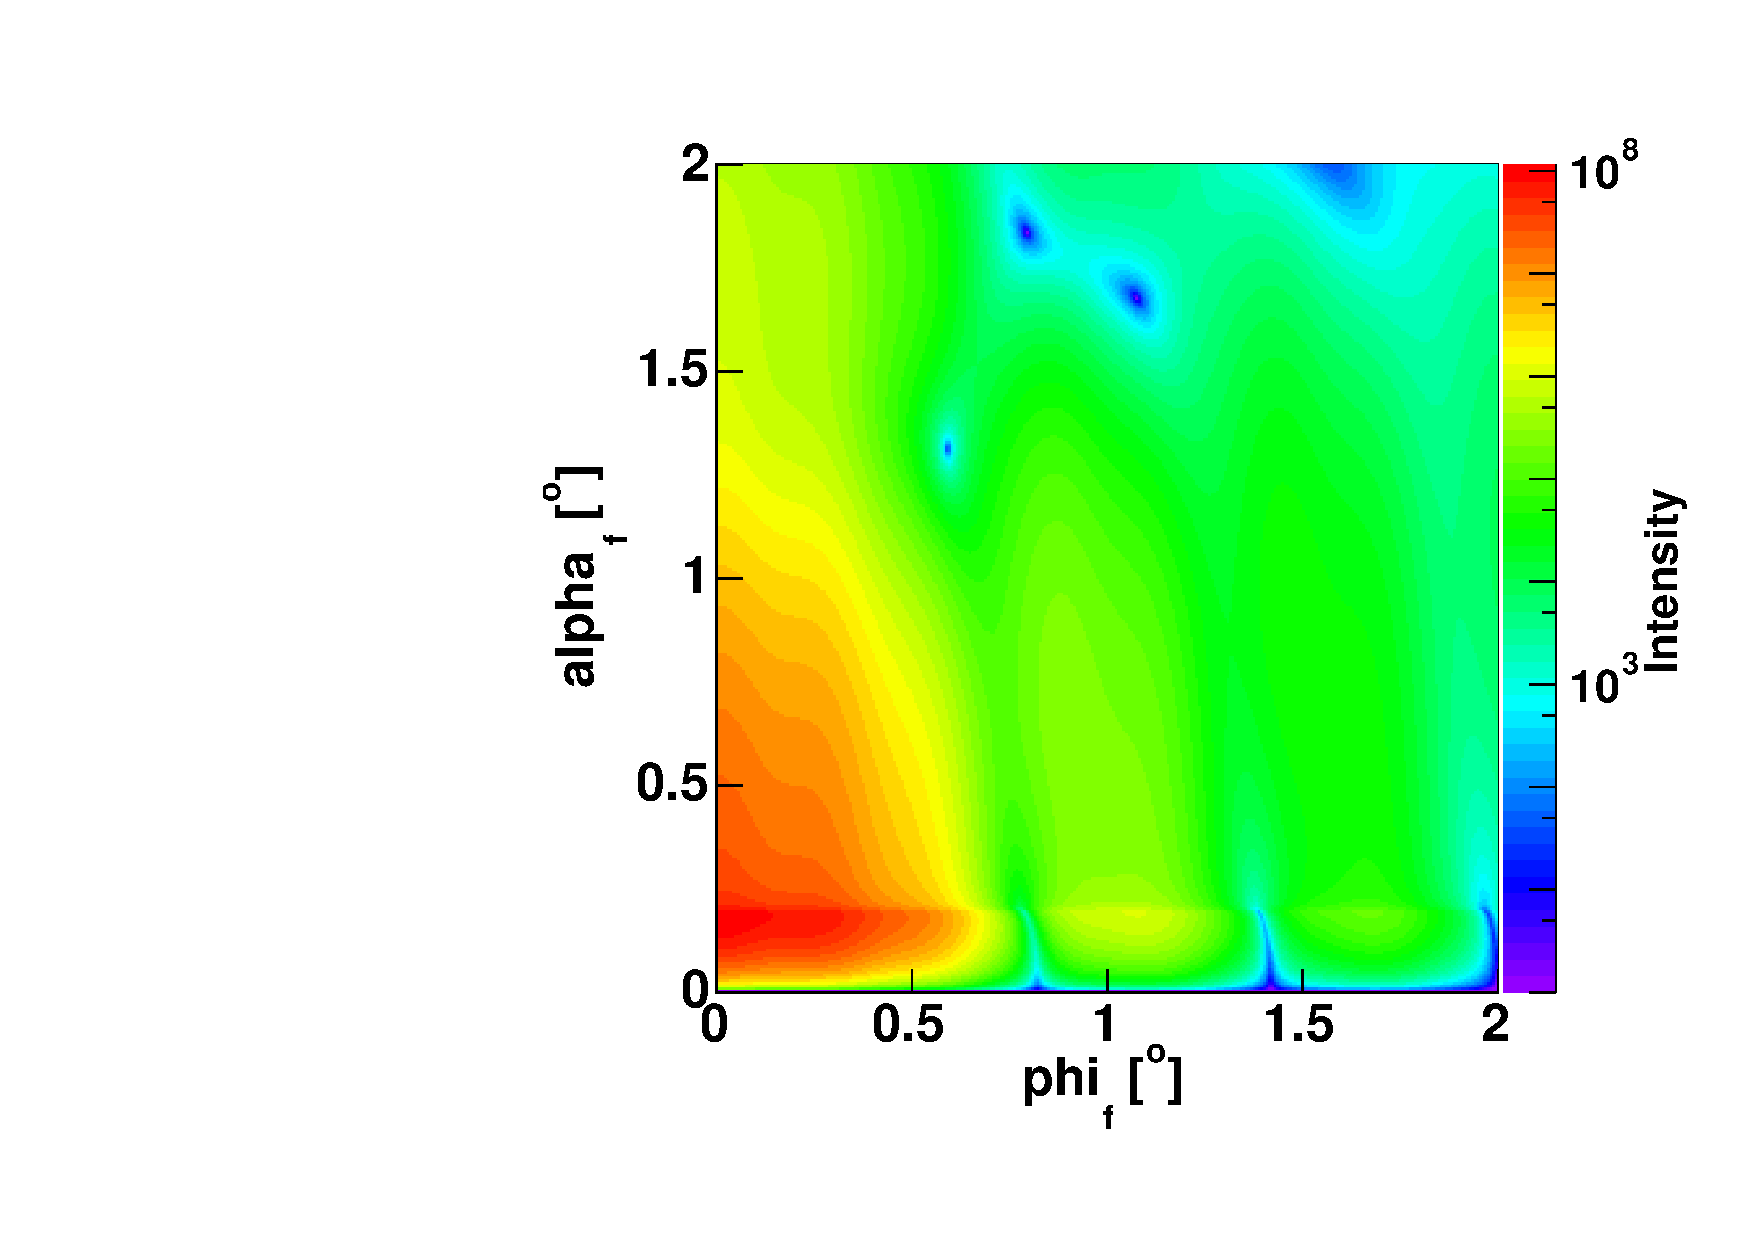
\includegraphics[angle=-90,width=0.5\textwidth]{fig/gisasmap/HSphere_2Dlattice.pdf}
\end{center}
\caption{Output intensity scattered from a sample made of half-spheres with 2DLattice interference function in the Decoupling Approximation.}
\label{fig:2dlatticeintensity}
\end{figure}

\FloatBarrier

\newpage%{\cleardoublepage}
%-------------------------------------------------------------------------------
\subsubsection{InterferenceFunction2DParaCrystal($L_1$, $L_2$, lattice\_angle, $xi$, damping\_length)} % TODO RESTORE \Code{}, \xi
%-------------------------------------------------------------------------------
\begin{itemize}
\item[where] $L_1$, $L_2$ are the lengths of the lattice cell,
\item[] lattice\_angle the angle between the lattice basis vectors $\mathbf{a}, \mathbf{b}$ in direct space,
\item[] $\xi$ is the angle defining the lattice orientation (set to $0$ by default).
\item[] \Code{damping\_length} is used to introduce finite size effects by applying a multiplicative coefficient equal to  $\exp$(-\Code{peak\_distance/damping\_length}) to the Fourier transform of the probability densities. \Code{damping\_length} is equal to 0 by default and, in this case, no correction is applied.
\end{itemize}
Two predefined interference functions can also be used:
\begin{itemize}
\item  \Code{createSquare(peak\_distance, damping\_length, domain\_size\_1, domain\_size\_2)}\\
where the angle between the base vectors of the lattice is set to $\pi/2$,
it creates a squared lattice,
\item \Code{createHexagonal(peak\_distance, damping\_length, domain\_size\_1, domain\_size\_2)}\\
where the angle between the base vectors of the lattice is set to $2\pi/3$ ,
\end{itemize}
where
\Code{domain\_size1, 2} are the dimensions of coherent domains of the paracrystal along the main axes,\\ \Code{peak\_distance} is the same in both directions and $\mathbf{a}\equiv \mathbf{x}$.\\

Probability distribution functions have to be defined. As the two-dimensional paracrystal is defined from two independent one-dimensional paracrystals, we need two of these functions, using\\ \Code{setProbabilityDistributions(pdf\_1, pdf\_2)}, with \Code{pdf\_{1,2}} related to each main axis of the paracrystal (see figure~\ref{fig:2dparaschematic}).


\begin{figure}[ht]
\begin{center}
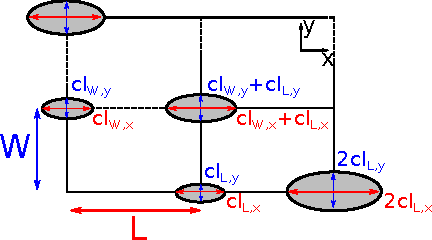
\includegraphics[width=0.75\textwidth]{fig/drawing/drawing2Dparacrystal.pdf}
\end{center}
\caption{Schematics of the ideal 2D paracrystal. The gray-shaded areas mark the regions where the probability to find a node is larger that the width at half-maximum of the distribution. $L$ and  $W$ are the mean inter-node distances along the two crystallographic axes. cl$_{(L,W),(x,y)}$ are the widths of the distribution of distance. The disorder is propagated as we add more nodes. Such a structure would be generated using \Code{InterferenceFunction2DParacrystal(L,W,90.*degrees,0,damp\_length)}, with \Code{pdf$_1$ = FTDistribution2DGauss(cl$_{L,x}$,cl$_{L,y}$)} and  \Code{pdf$_2$ = FTDistribution2DGauss(cl$_{W,x}$,cl$_{W,y}$)}.}
\label{fig:2dparaschematic}
\end{figure}


\paragraph{Example} The particles deposited on a substrate are half-spheres. The scattered beams interference via the 2DParacrystal distribution function. The paracrystal is based on a 2D hexagonal lattice with a Gaussian probability distribution function in reciprocal space.  Script~\ref{lst:2dparainterf} shows the implementation of the interference function and fig.~\ref{fig:2ddl} an example of output intensity using hemi-spherical particles.

\begin{lstlisting}[language=python, style=eclipseboxed,numbers=none,nolol,caption={\Code{Python} script to define a "2DParacrystal" interference function between particles forming an hexagonal monolayer. },label={lst:2dparainterf}]
    interference = InterferenceFunction2DParaCrystal.createHexagonal(30.0*nanometer,0.0, 40.0*micrometer, 40.0*micrometer)|
    pdf = FTDistribution2DCauchy(1.0*nanometer, 1.0*nanometer)
    interference.setProbabilityDistributions(pdf, pdf)
    particle_layout.addInterferenceFunction(interference)
\end{lstlisting}

\begin{figure}[ht]
\begin{center}
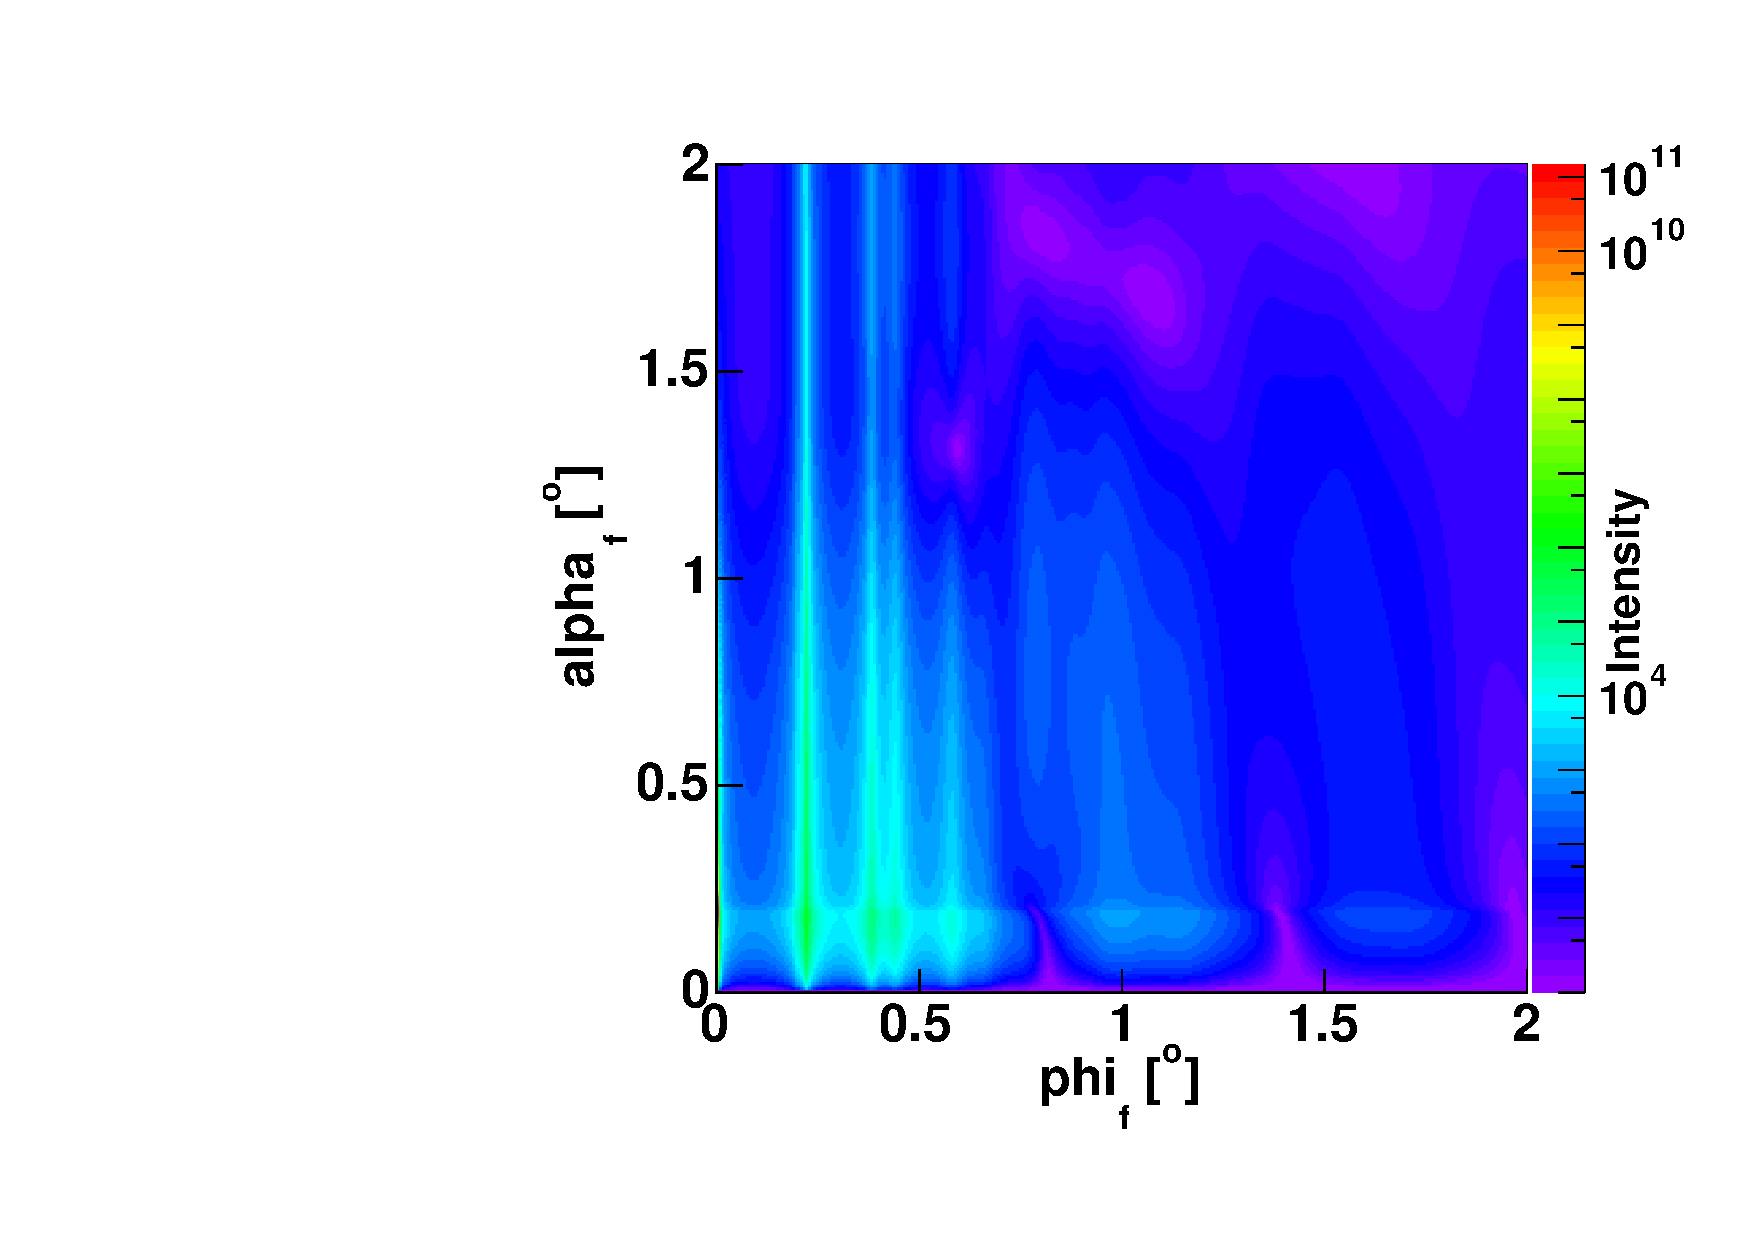
\includegraphics[angle=-90,width=0.5\textwidth]{fig/gisasmap/HSphere_2DDL.pdf}
\end{center}
\caption{Output intensity scattered from a sample made of half-spheres with 2DParacrystal interference function.}
\label{fig:2ddl}
\end{figure}

\FloatBarrier


%===============================================================================
\subsection{Summary}
%===============================================================================

\begin{table}[h]
  \scriptsize
\begin{tabular}{lll}
\hline
Name & Characteristics &  Comments \\
\hline
DA & no correlations& implemented with \Code{setApproximation} \\
     & & default option \\
\hline
LMA & sample = groups of particles & automatic implementation if several \\ 
 & of identical sizes and shapes & \Code{ParticleLayout}s are defined \\
\hline
SSCA & distance between particles =  &  - implemented with \Code{setApproximation} \\
 &function of their sizes&  - dimensionless coupling coefficient $\kappa$ is \\
 & & required using \Code{setKappa}.\\
\hline
\hline
\end{tabular}
\caption{List of size-distribution models implemented in \BornAgain.}
\end{table}

\begin{table}[h]
  \footnotesize
\begin{tabular}{lll}
\hline
Function  & Parameters & Comments\\
\hline
\Code{InterferenceFunctionNone}  & None & disordered distribution \\
\hline
\Code{InterferenceFunction1DLattice} & \Code{lattice\_length} & use only with infinitely long/wide particles \\
  & $\xi=\widehat{(\mathbf{x},\mathbf{a})}$ & pdf=(Cauchy, Gauss or Voigt)  to be defined\\
\hline
 \Code{InterferenceFunctionRadialParaCrystal}  & peak\_distance of pdf & pdf=(Cauchy, Gauss or Voigt) to be defined \\
& damping\_length (optional) & \\
\hline
 \Code{InterferenceFunction2DLattice}  & L\_1, L\_2: lattice lengths & pdf=(Cauchy, Gauss or Voigt) to be defined\\
                        & lattice\_angle=$\widehat{(\mathbf{a},\mathbf{b})}$ & \\
                                                            & $\xi =\widehat{(\mathbf{x},\mathbf{a})}$ & \\                                                  
\hline
\Code{InterferenceFunction2DParaCrystal}  & L\_1, L\_2: lattice lengths & 2D pdf=(Cauchy, Gauss or Voigt) to be defined \\
                          & lattice\_angle=$\widehat{(\mathbf{a},\mathbf{b})}$ & (1 pdf per axis) \\
& $\xi=\widehat{(\mathbf{x},\mathbf{a})}$ & \\
& damping\_length (optional)  &  same for both axes\\
\hline
\hline
\end{tabular}
\caption{List of interference functions implemented in \BornAgain. pdf : probability distribution function, $\mathbf{a}, \mathbf{b}$ are the lattice base vectors, and $\mathbf{x}$ is the axis vector perpendicular to the detector plane.}
\end{table}

%%%%%%%%%%%%%%%%%%%%%%%%%%%%%%%%%%%%%%%%%%%%%%%%%%%%%%%%%%%%%%%%%%%%%%%%%%%%%%%%
%%
%%   BornAgain User Manual
%%
%%   homepage:   http://www.bornagainproject.org
%%
%%   copyright:  Forschungszentrum Jülich GmbH 2015
%%
%%   license:    Creative Commons CC-BY-SA
%%   
%%   authors:    Scientific Computing Group at MLZ Garching
%%               C. Durniak, M. Ganeva, G. Pospelov, W. Van Herck, J. Wuttke
%%
%%%%%%%%%%%%%%%%%%%%%%%%%%%%%%%%%%%%%%%%%%%%%%%%%%%%%%%%%%%%%%%%%%%%%%%%%%%%%%%%


\chapter{Scattering by rough interfaces}  \label{sec:Roughness}

  ... to come

%%%%%%%%%%%%%%%%%%%%%%%%%%%%%%%%%%%%%%%%%%%%%%%%%%%%%%%%%%%%%%%%%%%%%%%%%%%%%%%%
%%
%%   BornAgain User Manual
%%
%%   homepage:   http://www.bornagainproject.org
%%
%%   copyright:  Forschungszentrum Jülich GmbH 2015
%%
%%   license:    Creative Commons CC-BY-SA
%%   
%%   authors:    Scientific Computing Group at MLZ Garching
%%               C. Durniak, M. Ganeva, G. Pospelov, W. Van Herck, J. Wuttke
%%
%%%%%%%%%%%%%%%%%%%%%%%%%%%%%%%%%%%%%%%%%%%%%%%%%%%%%%%%%%%%%%%%%%%%%%%%%%%%%%%%

\chapter{Polarized GISAS}  \label{sec:polTheory}

In this chapter,
we extend the theory
of grazing-incidence small-angle scattering (GISAS)
to X-rays and polarized neutrons.
We therefore need to study vectorial wave equations,
in contrast to the scalar theory of the previous chapter.

%===============================================================================
\section{X-ray propagation}\label{Sxray}
%===============================================================================
\index{Wave propagation!X-rays}
\index{X-rays!wave propagation}

.... to come ....


%===============================================================================
\section{Polarized neutrons}\label{Snpol}
%===============================================================================

\index{Neutrons!polarized}
\index{Polarization!neutrons}

.... to come ....


%%%%%%%%%%%%%%%%%%%%%%%%%%%%%%%%%%%%%%%%%%%%%%%%%%%%%%%%%%%%%%%%%%%%%%%%%%%%%%%%
%%
%%   BornAgain Physics Manual
%%
%%   homepage:   http://www.bornagainproject.org
%%
%%   copyright:  Forschungszentrum Jülich GmbH 2015-2020
%%
%%   license:    Creative Commons CC-BY-SA
%%
%%   authors:    Scientific Computing Group at MLZ Garching
%%
%%%%%%%%%%%%%%%%%%%%%%%%%%%%%%%%%%%%%%%%%%%%%%%%%%%%%%%%%%%%%%%%%%%%%%%%%%%%%%%%

\chapter{Instrument simulation}\label{SInstr}
\index{Instrument}

%%%%%%%%%%%%%%%%%%%%%%%%%%%%%%%%%%%%%%%%%%%%%%%%%%%%%%%%%%%%%%%%%%%%%%%%%%%%%%%%
\section{Incoming beam and resolution}\label{SBeam}
%%%%%%%%%%%%%%%%%%%%%%%%%%%%%%%%%%%%%%%%%%%%%%%%%%%%%%%%%%%%%%%%%%%%%%%%%%%%%%%%

\MissingSection

%%%%%%%%%%%%%%%%%%%%%%%%%%%%%%%%%%%%%%%%%%%%%%%%%%%%%%%%%%%%%%%%%%%%%%%%%%%%%%%%
\section{Detector images}\label{SdetImg}
%%%%%%%%%%%%%%%%%%%%%%%%%%%%%%%%%%%%%%%%%%%%%%%%%%%%%%%%%%%%%%%%%%%%%%%%%%%%%%%%

\def\tc{\text{c}}

%-------------------------------------------------------------------------------
\begin{figure}[t]
\begin{center}
\includegraphics[width=.5\textwidth]{fig/drawing/experimental_geometry.png}
\end{center}
\caption{Experimental geometry with a two-dimensional pixel detector.}
\label{FexpGeom}
\end{figure}
%-------------------------------------------------------------------------------

To conclude this chapter on the foundations of small-angle scattering,
we shall derive the geometric factors
that allow us to convert differential cross sections into detector counts.
We shall also discuss how to present data on a physically meaningful scale.

%===============================================================================
\subsection{Pixel coordinates, scattering angles, and $\mathbf{q}$ components}
%===============================================================================

We assume that scattered radiation is detected in a flat,
two-dimensional detector
that generates histograms on a rectangular grid,
consisting of $n\cdot m$ pixels of constant width and height,
as sketched in \cref{FexpGeom}.
This figure also shows the coordinate system
\index{Convention!coordinate system}%
\index{Coordinate system}%
according to unanimous GISAS convention,
with $z$ normal to the sample plane,
and with the incident beam in the $xz$ plane.
The origin is at the center of the sample surface.
We suppose that the detector is mounted perpendicular to the $x$ axis
at a distance $L$ from the sample position.
%the $x$ axis intersects the detector plane at $(L,y_\tc,z_\tc)$.
The real-space coordinate at the center of pixel $(i,j)$ is $(L,y_i,z_i)$.
Each pixel has a width~$\Delta y$ and a height~$\Delta z$.
\index{Detector!pixel coordinate}%
\index{Pixel|see {Detector}}%
BornAgain requires a full parametrization of the detector geometry
\index{Detector!calibration}%
to correctly perform the affine-linear mapping from pixel indices $i,j$
to pixel coordinates $x_i,y_i$;
see the \tuto{141}{rectangular detector tutorial}.
% TODO: link to Detector Reference

Since the differential scattering cross section \cref{Exsectiondef}
is given with respect to a solid-angle element $\d\Omega$,
we need to express the scattered wavevector $\k_\sf$ in spherical coordinates,
using the horizontal azimuth angle~$\phi_\sf$
and the vertical glancing angle $\alpha_\sf$.
The projection of $(\alpha_\sf,\phi_\sf)$ into
the detector plane~$(y,z)$ is known as the \E{gnomonic projection}.
\index{Gnomonic projection}%
\index{Projection!wavevector to pixel coordinate}%
\index{Mapping!wavevector to pixel coordinate}%
\index{Transformation!wavevector to pixel coordinate}%
From elementary trigonometry one finds
\begin{equation}\label{Eyzdet}
  \begin{array}{lcl}
  y &=& L \tan\phi_\sf,\\
  z &=& (L/ \cos\phi_\sf) \tan\alpha_\sf.
  \end{array}
\end{equation}
\cref{Fconstalphi} shows lines of equal $\alpha_\sf$,~$\phi_\sf$
in the detector plane.
To emphasize the curvature of the constant-$\alpha_\sf$ lines,
scattering angles up to more than 25$^\circ$ are shown.
In typical SAS or GISAS,
scattering angles are much smaller,
and therefore the mapping between pixel coordinates and
scattering angles is in a good first approximation linear.
Of course \BornAgain\ is not restricted to this linear regime,
but uses the exact nonlinear mapping~\cref{Eyzdet}.

%-------------------------------------------------------------------------------
\begin{figure}[t]
\begin{center}
\includegraphics[width=.47\textwidth]{fig/drawing/SAS_const_alphi.ps}
\end{center}
\caption{Lines of constant $\alpha_\sf$ (red) or $\phi_\sf$ (blue)
in the detector plane,
for a planar detector at distance~$L$ from the sample.
The black dot indicates the beamstop location for
the central incident beam (SAS geometry, $\hat\k_\si = \hat x$).}
\label{Fconstalphi}
\end{figure}
%-------------------------------------------------------------------------------

To determine the scattering vector $\q_{ij}$
that corresponds to a pixel $(i,j)$,
we need to express the outgoing wavevector~$\k_\sf$ as function of $y$ and~$z$.
This can be done either by inverting \cref{Eyzdet}
and inserting the so obtained $\alpha_\sf(y,z)$ and $\phi_\sf(y)$ in
\begin{equation}\label{Ekf_by_angle}
  \k_\sf=K\left(\begin{array}{c}
   \cos\alpha_\sf\cos\phi_\sf\\
   \cos\alpha_\sf\sin\phi_\sf\\
   \sin\alpha_\sf\end{array}\right),
\end{equation}
or much more directly by using geometric similarity in Cartesian coordinates.
The result is rather simple:
\begin{equation}\label{Ekf_by_pixel}
  \k_\sf=\frac{K}{\sqrt{L^2+y^2+z^2}}\left(\begin{array}{c}
   L\\
   y\\
   z\end{array}\right).
\end{equation}


%-------------------------------------------------------------------------------
\begin{figure}[t]
\begin{center}
\includegraphics[width=.47\textwidth]{fig/drawing/SAS_const_q_x.ps}
\hfill
\includegraphics[width=.47\textwidth]{fig/drawing/SAS_const_q_yz.ps}
\end{center}
\caption{Lines of constant $q_x$ (left), $q_y$ or $q_z$ (right),
in units of the incident wavenumber $K=2\pi/\lambda$,
for a planar detector.
SAS geometry as in Fig.~\protect\ref{Fconstalphi}.}
\label{Fconstq}
\end{figure}
%-------------------------------------------------------------------------------

The transform \cref{Eqalgo} between pixel coordinates $y$,~$z$
and physical scattering vector components $q_y$, $q_z$
is nonlinear, due to the square-root term in the denominator of~\cref{Ekf_by_pixel}.
For $y,z\ll L$, however, nonlinear terms loose importance.

%-------------------------------------------------------------------------------
\begin{figure}[t]
\begin{center}
\includegraphics[width=1\textwidth]{fig/gisasmap/ff_det_box.pdf}
\end{center}
\caption{Simulated detector image for small-angle scattering from
uncorrelated cuboids (right rectangular prisms).
  \index{Box (form factor)}
  \index{Cuboid (form factor)}
  \index{Prism (form factor)!reactangular (Box)}
  \index{FormFactorBox@\Code{FormFactorBox}}
The incoming wavelength is 0.1~nm.
The prisms have edge lengths $L_y=L_z=10$~nm;
the length $L_x$, in beam direction, is varied as shown above the plots.
\index{Circular modulation}%
The circular modulation comes from a factor $\sinc(q_x L_x/2)$
in the cuboid form factor, with $q_x$ given by~\cref{Eqxasy}.}
\label{Fdetbox}
\end{figure}
%-------------------------------------------------------------------------------

The left detector frame in \cref{Fconstq}
shows circles of constant values of $\pm q_x$.
For given steps in $q_x$, the distance between adjacent circles
increases towards the detector center.
From \cref{Eq} and \cref{Ekf_by_pixel},
one finds asymptotically for $y,z\to L$
that $q_x$ goes with the square of the two other components of the scattering vector,
\begin{equation}\label{Eqxasy}
  \frac{q_x}{K}
  \doteq \frac{y^2+z^2}{2 L^2}
  \doteq \frac{q_y^2 + q_z^2}{2K^2}.
\end{equation}
Therefore, under typical small angle conditions $y,z\to L$
the dependence of the scattering signal on $q_x$ is unimportant:
one basically measures $v(\q)\simeq v(0,q_y,q_z)$.
The exception, for sample structures with long correlations in $x$~direction,
is illustrated in~\cref{Fdetbox}.

%-------------------------------------------------------------------------------
\begin{figure}[t]
\begin{center}
\includegraphics[width=.47\textwidth]{fig/drawing/SAS_const_p_yz.ps}
\end{center}
\caption{The outer contour of the blue and red grid
shows the border of a square detector image
after transformation into the physical coordinates $q_y$,~$q_z$.
The blue and red curves correspond to horizontal and vertical lines in the detector.}
\label{Fconstp}
\end{figure}
%-------------------------------------------------------------------------------

As anticipated in \cref{Eqxasy},
the other two components of $\q$ are in first order linear in the pixel coordinates,
\begin{equation}
  \frac{q_y}{K}=\frac{y}{L}\left(1-\frac{y^2+z^2}{2L^2}+\ldots\right),
\end{equation}
and similarly for~$q_z$.
The nonlinear correction terms lead to the pincushion distortion
shown in the right detector frame in \cref{Fconstq}.
\index{Distortion!of $q_x$, $q_y$ grid in detector plane}%
\index{Detector!distortion of $q_x$, $q_y$ grid}%
\index{Pincushion distortion}%

Since pixel coordinates are meaningful only
with respect to a specific experimental setup,
users may wish to transform detector images
towards the physical coordinates $q_y$ and~$q_z$.
As shown in \cref{Fconstp},
this would yield a barrel-shaped illuminated area
in the $q_y$,~$q_z$~plane.

To summarize this section,
the wavevector $\q_{ij}$ can be determined from the pixel indices
through the following steps:
\begin{equation}\label{Eqalgo}
  \begin{array}{cl}
      (i,j)&\\
      \downarrow&\mbox{calibrate of origin, then employ affine-linear mapping}\\
      (y,z)\\
      \downarrow&\mbox{use (\protect\ref{Ekf_by_pixel})}\\
      \k_\sf&\\
      \downarrow&\mbox{use (\protect\ref{Eq})}\\
      \q&\\
  \end{array}
\end{equation}

\Note{\indent Transforming detector images
  from pixel coordinates into the $q_y$,~$q_z$~plane is not implemented in \BornAgain,
  and not on our agenda.
  We would, however, like to hear about use cases.}

\indent When simulating and fitting experimental data with \BornAgain,
detector images remain unchanged.
All work is done in terms of reduced pixel coordinates $y/L$ and~$z/L$.
Corrections are applied to the simulated, not to the measured data.

\Work{\indent \ldots show how to plot $q$ grid on top of detector image \ldots}

%===============================================================================
\subsection{Intensity transformation}
%===============================================================================

The solid angle under which a detector pixel
is illuminated from the sample is in linear approximation
\begin{equation}
  \Delta\Omega
  = \cos\alpha_\sf\:\Delta\alpha_\sf\,\Delta\phi_\sf
  = \cos\alpha_\sf
    \left|\frac{\partial(\alpha_\sf,\phi_\sf)}{\partial(y,z)}\right|
    \Delta y \,\Delta z
  = \cos^3\!\alpha_\sf\, \cos^3\!\phi_\sf\: \frac{\Delta y \,\Delta z}{L^2}.
\end{equation}
\index{Detector!illumination angle correction factor}%
\index{Illumination!detector}%
Altogether,
the expected count rate in detector pixel $(i,j)$ is proportional to
\begin{equation}\label{EItrafo_cos}
  I_{ij} = \cos^3\!\alpha_\sf\, \cos^3\!\phi_\sf\:
          \frac{\d\sigma}{\d\Omega}(\q_{ij}),
\end{equation}
where we have omitted constant factors $L^{-2}$, $\Delta y$ and $\Delta z$.
Using pixel coordinates instead of angles, this can be rewritten as
\begin{equation}\label{EItrafo_pix}
  I_{ij} = \left( 1+\frac{y^2+z^2}{L^2}\right)^{-3/2}
          \frac{\d\sigma}{\d\Omega}\bigl(\q_{ij}(y,z)\bigr).
\end{equation}
%(usually as the centre between the transmitted
%and the specularly reflected beam spot).

%Tradition wants that raw data be \E{treated} or \E{reduced}
%before they are \E{analyzed}.
%In our case, raw data reduction would comprise
%the transform \cref{Eqalgo} of pixel coordinates into scattering vectors,
%and the accompanying renormalization \cref{EItrafo} of pixel counts.


%%%% Part II: Reference
%%%%%%%%%%%%%%%%%%%%%%%%%%%%%%%%%%%%%%%%%%%%%%%%%%%%%%%%%%%%%%%%%%%%%%%%%%%%%%%%
%%
%%   BornAgain User Manual
%%
%%   homepage:   http://www.bornagainproject.org
%%
%%   copyright:  Forschungszentrum Jülich GmbH 2016
%%
%%   license:    Creative Commons CC-BY-SA
%%
%%   authors:    Scientific Computing Group at MLZ Garching
%%               M. Ganeva, G. Pospelov, W. Van Herck, J. Wuttke
%%
%%%%%%%%%%%%%%%%%%%%%%%%%%%%%%%%%%%%%%%%%%%%%%%%%%%%%%%%%%%%%%%%%%%%%%%%%%%%%%%%

\part{Reference}\label{PREF}

\chapter{Introduction: The three interfaces of \BornAgain}  \label{sec:API3}

%%%%%%%%%%%%%%%%%%%%%%%%%%%%%%%%%%%%%%%%%%%%%%%%%%%%%%%%%%%%%%%%%%%%%%%%%%%%%%%%
\section{Architectural overview}
%%%%%%%%%%%%%%%%%%%%%%%%%%%%%%%%%%%%%%%%%%%%%%%%%%%%%%%%%%%%%%%%%%%%%%%%%%%%%%%%

The overall architecture of \BornAgain\ is outlined in \cref{Farch1}.
The core of \BornAgain\
\index{Core|see {\Code{libBornAgainCore}}}
comprises functionality to construct arbitrary hierarchical sample models,
to setup instrument models,
and to compute the expected detector image for any given sample and instrument model.
Furthermore \BornAgain\ comes with various minimizers that optimize model parameters
to fit the simulated detector image to a given experimental image.
All this functionality is implemented in a library, \Code{libBornAgainCore}.

\begin{figure}[tbh]
\begin{center}
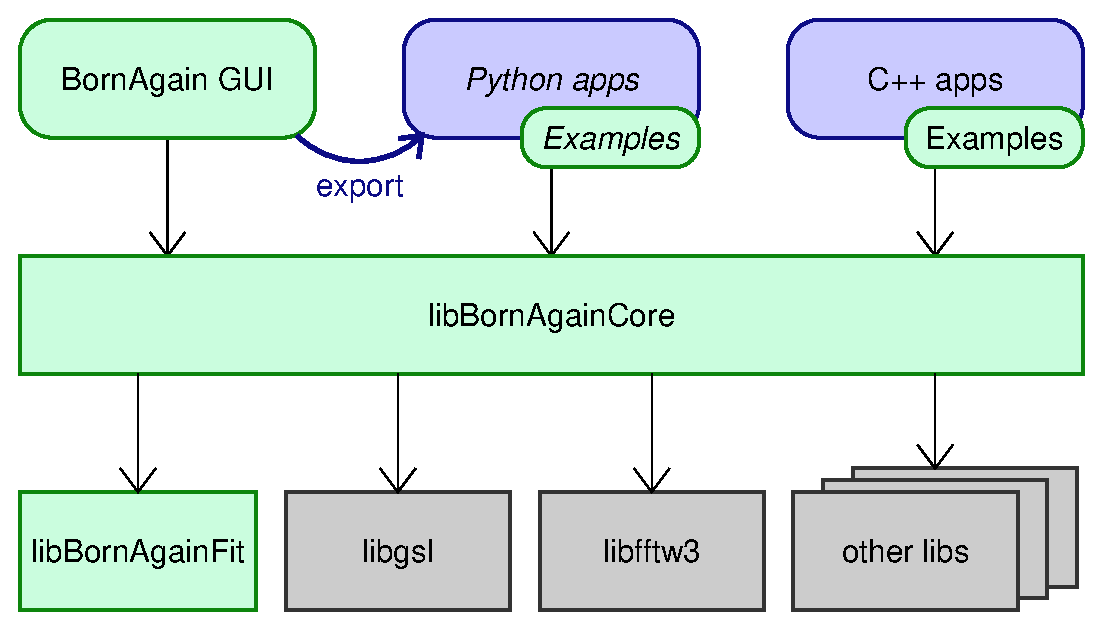
\includegraphics[width=0.7\textwidth]{fig/drawing/architecture1.ps}
\end{center}
\caption{Overall architecture of \BornAgain.
\index{Architecture!applications and libraries}%
Applications are shown as oval fields, libraries as rectangles.
Black arrows indicate ``depends on''.
Green fields designate software that is part of \BornAgain.
Gray fields are external dependences
(only two external libraries are explicitly shown;
several more are listed in the online compilation instructions).
Blue fields indicate stand-alone applications that use \BornAgain's
two Application Programming Interfaces (the C$++$ API and the Python API).
\index{C++!using BornAgain from}
\index{Python!using BornAgain from}
\index{Application Programming Interface}
While such applications are to be written by users,
some examples come with the \BornAgain\ source distribution,
and are explained in the following Manual chapters.
It is also possible to export a simulation setup from GUI as Python code.
The binding of C++ to Python is highly simplified here.
For a more accurate picture, see \Cref{FarchPy}.}
\label{Farch1}
\end{figure}

\index{libBornAgainCore@\Code{libBornAgainCore}}
This library, in turn, depends on a number of other libraries.
One of these, the minimizer wrapper \Code{libBornAgainFit}
\index{libBornAgainFit@\Code{libBornAgainFit}}
\index{Minimizers|see \Code{libBornAgainFit}}
has been written specifically for use in \BornAgain,
and for the time being is only distributed as part of \BornAgain,
though in the future it may find applications in other contexts.
The other library dependences of \Code{libBornAgainCore}
are multi-purpose libraries that are easily available as open-source packages.
\index{Dependences!libraries}

The library \Code{libBornAgainCore} can be used in three different ways:
From its graphical user interface (GUI), or
from user-written stand-alone applications in the programming languages C$++$ or Python.
These different approaches are briefly outlined below.
The Python interface is then described at length in the next chapters.

%%%%%%%%%%%%%%%%%%%%%%%%%%%%%%%%%%%%%%%%%%%%%%%%%%%%%%%%%%%%%%%%%%%%%%%%%%%%%%%%
\section{Using \BornAgain\ from its Graphical User Interface}
%%%%%%%%%%%%%%%%%%%%%%%%%%%%%%%%%%%%%%%%%%%%%%%%%%%%%%%%%%%%%%%%%%%%%%%%%%%%%%%%
\index{Graphical User Interface|(}
\index{bornagain@\Code{bornagain}|see {Graphical User Interface}}
\index{Exectutable!bornagain@\Code{bornagain}|see {Graphical User Interface}}
\index{Binary|see {Executable}}
%\index{Project name!BornAgain@\BornAgain}

The project \BornAgain\ comes with a stand-alone application called \Code{bornagain}
that provides a Graphical User Interface (GUI).
Note that we distinguish between the GUI executable \Code{bornagain},
the underlying library \Code{libBornAgainCore}, and the project \BornAgain\ at large.

The GUI allows users to quickly setup a simulation, to visualize simulated
detector images, to compare with experimental images, and to run fits.
It provides comfortable access to much, but not all the functionality
of \Code{libBornAgainCore}.
Depending on application fields,
users may sooner or later reach the limits of current GUI support.
Other users may have repetitive tasks that are cumbersome under a GUI.
In such cases, users can export their sample and instrument models from
the GUI as a Python script,
and continue work by directly editing the Python code.
\index{Export!Python from GUI}

See the online documentation for
\tuto{18}{detailed instructions} how to use the GUI.
\index{Graphical User Interface|)}

%%%%%%%%%%%%%%%%%%%%%%%%%%%%%%%%%%%%%%%%%%%%%%%%%%%%%%%%%%%%%%%%%%%%%%%%%%%%%%%%
\section{Using \BornAgain\ from Python}
%%%%%%%%%%%%%%%%%%%%%%%%%%%%%%%%%%%%%%%%%%%%%%%%%%%%%%%%%%%%%%%%%%%%%%%%%%%%%%%%
\index{Python!using BornAgain from|(}
\index{Application Programming Interface!Python|(}

\BornAgain\ simulations and fits can be set up and run from Python programs
or from a Python command-line interpreter like \Code{IPython}.
\index{IPython}
\index{Command line!Python}
A short program in an interpreted language like Python is customarily called
\index{Script!Python}
\index{Python!script}
a \E{script},
and therefore in the following we will talk about \E{Python scripts}.
Of course this does not preclude the possibility that such scripts evolve into
complex programs, modules, or packages.
And anything we say about scripts also applies to usage of \BornAgain\ in an
interactive Python session.%
\index{Interactive Python session}%
\index{Python!interactive use}%

Usage of \BornAgain\ in a Python script should start with the command
\setPy
\begin{lstlisting}
import bornagain as ba @\label{import_as}\index{Import!\BornAgain\ to Python|(}@
\end{lstlisting}
This then allows calls to \BornAgain\ in commands like
\pagebreak[2]
\setPyNum
\begin{lstlisting}
air = ba.HomogeneousMaterial("Air", 0.0, 0.0) @\label{constructor_beg}@
air_layer = ba.Layer(air)
sample = ba.MultiLayer() @\label{constructor_end}@
sample.addLayer(air_layer) @\label{class_func_call}@
\end{lstlisting}
The function calls in lines \ref{constructor_beg}--\ref{constructor_end}
return new \E{objects}.
\index{Object!constructor}
These objects are instances of \E{classes} defined in \BornAgain.
\index{Class!Instantiation}
In the language of object-oriented programming,
a Function that returns a new instance of a class is called a \E{constructor}.
\index{Constructor}
In Python, as in C++, constructor names coincide with class names;
so the constructor function \Code{Layer(material)} will return an
object of class type \Code{Layer}.

\begin{figure}[tb]
\begin{center}
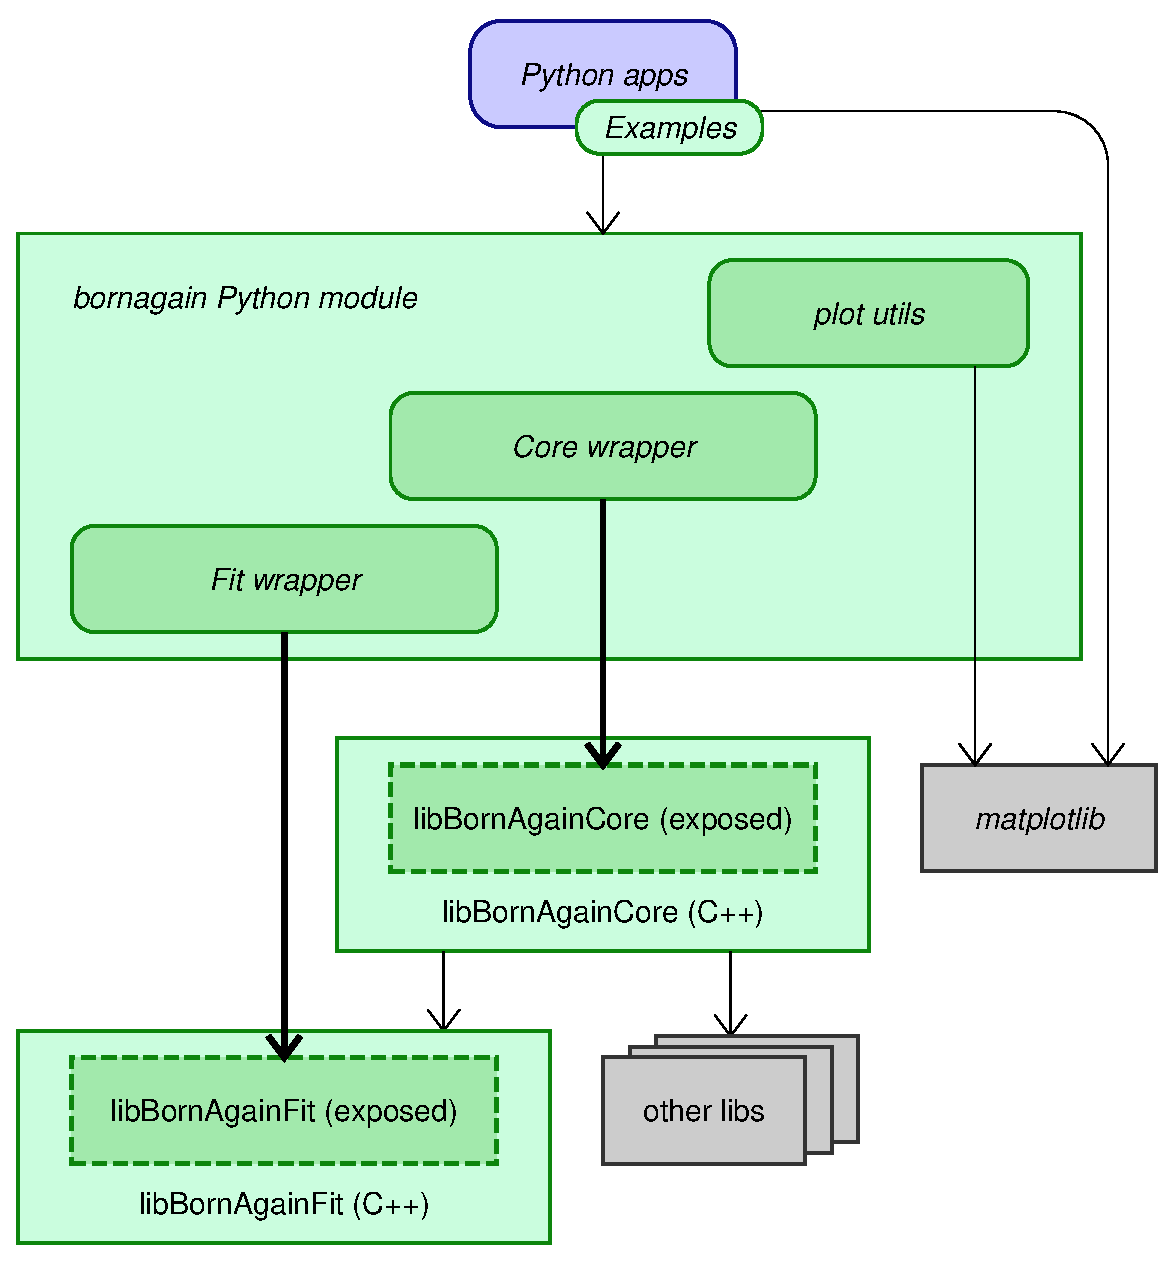
\includegraphics[width=0.72\textwidth]{fig/drawing/architecturePy.ps}
\end{center}
\caption{Relation between the BornAgain C++ libraries and the Python layer.
\index{Architecture!Python binding}%
Python code is indicated by \textsl{slanted font}.
Colors as in \Cref{Farch1}.
Bold arrows indicate ``depends on'' for code that is automatically generated
by the software tool Swig.%
\index{Swig}%
\index{Python!Swig}%
}
\label{FarchPy}
\end{figure}

To prevent accidental use of class or constructor names,
they are encapsulated in a \E{namespace}
\index{Namespace}
called \Code{bornagain}.
The \Code{import} command in the above code line~\ref{import_as}
makes this namespace available under the shortcut \Code{ba}.
\index{Import!\BornAgain\ to Python|)}
Note, however, that not all calls to \BornAgain\ require
(and can be recognized by) the prefix \Code{ba}.
The function call \Code{addLayer} in line~\ref{class_func_call}
is defined inside the \BornAgain\ class \Code{MultiLayer}.
The programmer is supposed to know that \Code{sample} is an instance of
class \Code{MultiLayer}, which is part of \BornAgain.
Therefore, there is no need (and no way) to adorn function calls like \Code{addLayer}
with the namespace label \Code{ba}.

The entirety of classes and functions provided by \BornAgain\
and exposed to Python forms the \E{BornAgain Python API}.
An API (Application Programming Interface)
\index{Application Programming Interface!Python}
is a kind of protocol that tells a programmer how to use a library.
In this perspective, the research scientist
who uses Python to set up simulations or fits
is seen as a \E{programmer} who writes an application program.
This notwithstanding, he is still a \E{user}
of the BornAgain Python library.
The relation of this library to the underlying C++ library is explained
in \Cref{FarchPy}.
The classes and functions in the BornAgain Python library have the same
names, argument lists, and return values
as their counterparts in the C++ library.
Therefore, we provide references only for the latter,
which has the advantage that it is more explicit about the data types
of function arguments and return values.

\index{Application Programming Interface!Python|)}
\index{Python!using BornAgain from|)}

%%%%%%%%%%%%%%%%%%%%%%%%%%%%%%%%%%%%%%%%%%%%%%%%%%%%%%%%%%%%%%%%%%%%%%%%%%%%%%%%
\section{Using \BornAgain\ from C++}
%%%%%%%%%%%%%%%%%%%%%%%%%%%%%%%%%%%%%%%%%%%%%%%%%%%%%%%%%%%%%%%%%%%%%%%%%%%%%%%%
\index{C++!using BornAgain from|(}
\index{Application Programming Interface!C++|(}

Alternatively, BornAgain can also be used from the programs written
in the language~C++.
Since BornAgain itself is written in C++,
\index{C++!BornAgain written in}%
the BornAgain C++ API natively consists of
all classes and functions in \Code{libBornAgainCore} and \Code{libBornAgainFit},
\index{libBornAgainCore@\Code{libBornAgainCore}}%
\index{libBornAgainFit@\Code{libBornAgainFit}}%
including internal ones that are not exposed to Python.
It empowers application programmers to use BornAgain
in ways we cannot foresee.

Normal GISAS users, however, will find that their simulation and fit tasks
are well served by the Python API,
that edit-and-rerun cycles are faster with Python than with a compiled language,
and that there is no need to use BornAgain from C++.
Therefore, we provide only one code example:
\url{Examples/cpp/CylindersAndPrisms} in the source distribution.

The C++ API is fully documented
in the automatically generated Doxygen reference at
\url{http://apps.jcns.fz-juelich.de/doxy/BornAgain/index.html}.
\index{Doxygen!API reference}
\index{C++!Doxygen API reference}
The remaining chapters of this Manual
provide a selective, annotated reference,
especially of functions related to the physical modelling.
It is organized top-down: We start with top-level classes like
\texttt{GISAS\-Simulation};
then we explain the classes needed to set up a meaningful simulation.
For an alphabetic lookup of classes and functions,
see the general Index at the end of this Manual.
For classes and functions not explained here,
see the Doxygen documentation.

\index{Application Programming Interface!C++|)}
\index{C++!using BornAgain from|)}

%%%%%%%%%%%%%%%%%%%%%%%%%%%%%%%%%%%%%%%%%%%%%%%%%%%%%%%%%%%%%%%%%%%%%%%%%%%%%%%%
%%
%%   BornAgain User Manual
%%
%%   homepage:   http://www.bornagainproject.org
%%
%%   copyright:  Forschungszentrum Jülich GmbH 2015
%%
%%   license:    Creative Commons CC-BY-SA
%%
%%   authors:    Scientific Computing Group at MLZ Garching
%%               C. Durniak, M. Ganeva, G. Pospelov, W. Van Herck, J. Wuttke
%%
%%%%%%%%%%%%%%%%%%%%%%%%%%%%%%%%%%%%%%%%%%%%%%%%%%%%%%%%%%%%%%%%%%%%%%%%%%%%%%%%

% \part{Reference}\label{PREF}

\chapter{Simulation, Instrument, Histograms}\label{SRefBas}

%%%%%%%%%%%%%%%%%%%%%%%%%%%%%%%%%%%%%%%%%%%%%%%%%%%%%%%%%%%%%%%%%%%%%%%%%%%%%%%%
\section{Simulation classes}\label{SRefSim}
%%%%%%%%%%%%%%%%%%%%%%%%%%%%%%%%%%%%%%%%%%%%%%%%%%%%%%%%%%%%%%%%%%%%%%%%%%%%%%%%

Each BornAgain simulation is run from one of the three
foundational simulation classes:\footnote
{Developer note: They all inherit from a common non-public (pure virtual)
interface class \ttIdx{Simulation}.}
\ttIdx{GISAS\-Simulation},
\ttIdx{OffSpecularSimulation},
\ttIdx{SpecularSimulation}.

%===============================================================================
\subsection{GISAS\-Simulation}
%===============================================================================

Class \ttIdx{GISAS\-Simulation} controls one
grazing-incidence small-angle scattering simulation.
The following six functions from the C$++$ API are sufficient to set up and run a basic
simulation:
\setCpp
\begin{lstlisting}
class GISASSimulation {
  GISASSimulation(); // constructor
  void setDetectorParameters(...);
  void setBeamParameters(...);
  void setSample(...);
  void runSimulation();
  Histogram2D* getIntensityData(...);
};
\end{lstlisting}
\constrHide{GISAS\-Simulation}%
They shall now be explained with full signatures.
Some alternatives will also be shown.

%--------------------------------------------------------------------------------
\begin{figure}[tb]
\begin{center}
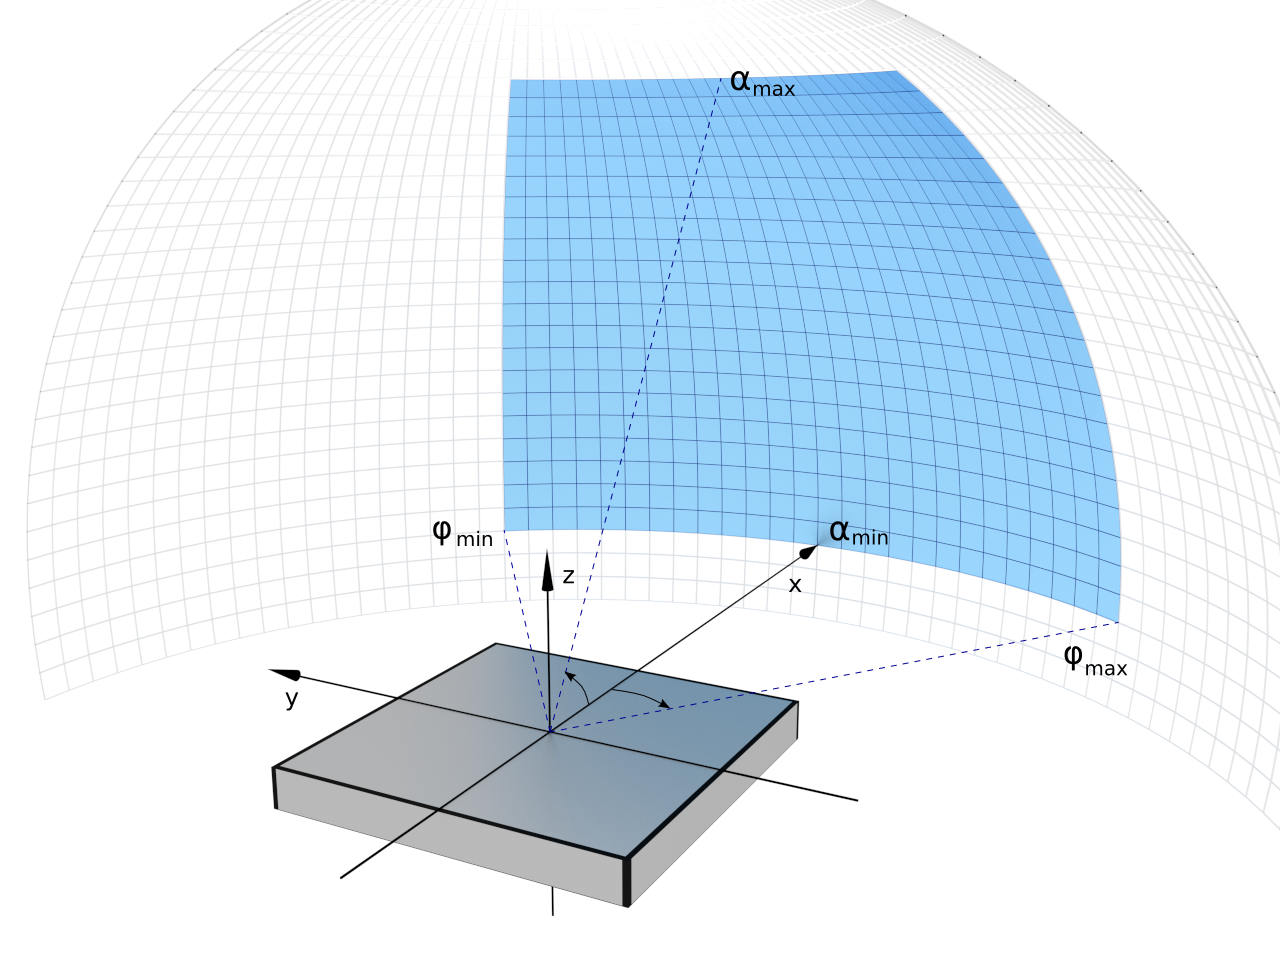
\includegraphics[width=0.7\textwidth]{fig/drawing/gisas_spherical_detector.png}
\end{center}
\caption{A spherical detector, with geometric conventions for polar angles~$\alpha$
and azimuthal angles~$\varphi$}
\label{FDetSpher}
\end{figure}
%--------------------------------------------------------------------------------

A two-dimensional detector must be defined through on of the following calls:

\subsubsection{Detector setup}\label{SRefDet}
\begin{lstlisting}
class GISASSimulation {
  void setDetectorParameters(
    size_t n_phi,   double phi_min,   double phi_max,
    size_t n_alpha, double alpha_min, double alpha_max);
  void setDetector(const IDetector2D& detector);
};
\end{lstlisting}
The function \clFct{GISAS\-Simulation}{setDetectorParameters}
defines a \ttIdx{SphericalDetector}
\index{Detector!spherical}%
with \texttt{n\_phi} equidistant azimuthal ($xy$, horizontal, off-specular) bins
\index{Azimuthal angle}%
\index{Horizontal angle}%
\index{Off-specular angle}%
\index{Angle!azimuthal ($=$ horizontal)}%
and  \texttt{n\_alpha} equidistant polar ($xz$, vertical, specular) bins (\cref{FDetSpher}).
\index{Polar angle}%
\index{Vertical angle}%
\index{Specular angle}%
\index{Angle!polar ($=$ vertical)}%

The alternate function~\clFct{GISAS\-Simulation}{setDetector}
allows to supply any detector that realizes the interface \ttIdx{IDetector2D}.
Besides \texttt{SphericalDetector}, this can be a \ttIdx{Rectangular\-Detector}.
For details, see the \tuto{141}{rectangular detector tutorial}.

\subsubsection{Beam setup}\label{SRefBeam}
\begin{lstlisting}
class GISASSimulation {
  void setBeamParameters(
    double wavelength, double alpha_i, double phi_i);
};
\end{lstlisting}
This function\clFctHide{GISAS\-Simulation}{setBeamParameters}
is rather self-explanatory.
The incident radiation wavelength must be given in the same length unit
that is also used in the sample description.

\subsubsection{Sample setup}
\begin{lstlisting}
class GISASSimulation {
  GISASSimulation(const MultiLayer& p_sample);
  GISASSimulation(const std::shared_ptr<IMultiLayerBuilder> p_sample_builder);
  void setSample(const MultiLayer& sample);
  void setSampleBuilder(const std::shared_ptr<IMultiLayerBuilder> p_sample_builder);
};
\end{lstlisting}
Besides function \clFct{GISAS\-Simulation}{setSample}, there is an alternate
function \clFct{GISAS\-Simulation}{setSampleBuilder}.
Either function call can be replaced by an extend forms of the constructor
\constr{GISAS\-Simulation}.

Since BornAgain is only concerned with multilayer samples,
the \E{sample} class
\index{Sample (class)|see{\Code{MultiLayer}}}%
is called \ttIdx{MultiLayer},
and each \E{sample builder} must realize the interface \ttIdx{IMulti\-Layer\-Builder}.
\index{Sample builder (interface)|see{\Code{IMultiLayerBuilder}}}%

A sample builder provides a more versatile way to define a sample.
Usage examples can be found in the test cases in \ttIdx{Core/StandardSamples}
and in the Python example \ttIdx{FitSpheresInHexLattice\_builder.py}.

\subsubsection{Execution}
\begin{lstlisting}
class GISASSimulation {
  void runSimulation();
};
\end{lstlisting}
\clFctHide{GISAS\-Simulation}{runSimulation}%
Once the simulation is fully set up, it is run once through this command.
Results are stored in a protected class variable.

\subsubsection{Retrieval of result}
\begin{lstlisting}
class GISASSimulation {
  Histogram2D* getIntensityData(IDetector2D::EAxesUnits units_type = IDetector2D::DEFAULT) const;
};
\end{lstlisting}
\clFctHide{GISAS\-Simulation}{getIntensityData}%
This function returns a pointer to a \ttIdx{Histogram2D}
that contains the outcome of the simulation.
% TODO link -> as further discussed in~\Cref{SRefHis2D}.

%===============================================================================
\subsection{Off\-Specular\-Simulation}
%===============================================================================

\MissingSection

%===============================================================================
\subsection{Specular\-Simulation}
%===============================================================================

\MissingSection

%%%%%%%%%%%%%%%%%%%%%%%%%%%%%%%%%%%%%%%%%%%%%%%%%%%%%%%%%%%%%%%%%%%%%%%%%%%%%%%%
\section{Intensity data}
%%%%%%%%%%%%%%%%%%%%%%%%%%%%%%%%%%%%%%%%%%%%%%%%%%%%%%%%%%%%%%%%%%%%%%%%%%%%%%%%

\MissingSection
\iffalse

%===============================================================================
\subsection{Histogram2D}\label{SRefHis2D}
%===============================================================================

\Work{The following material has been moved here from a Tutorial.
It still needs to be recast in Reference style.}

The \Code{IntensityData} object stores the
simulated or real intensity data together with the axes definition of the detector in BornAgain's internal format.
During the simulation setup
it is created automatically when the user specifies the detector characteristics and is filled with the simulated intensities after the simulation is completed.

\setPy
\begin{lstlisting}
simulation = Simulation()
simulation.setDetectorParameters(10, -5.0*degree, 5.0*degree, 5, 0.0*degree, 1.0*degree)
...
simulation.runSimulation()
intensity = simulation.getIntensityData() @\label{py:UserApi:intensity}@
\end{lstlisting}

The \Code{IntensityData} object retrieved in line~\ref{py:UserApi:intensity} corresponds to
the two dimensional detector pixel array as shown in \cref{fig:UserApi:IntensityData}.

\begin{figure}[ht]
  \centering
    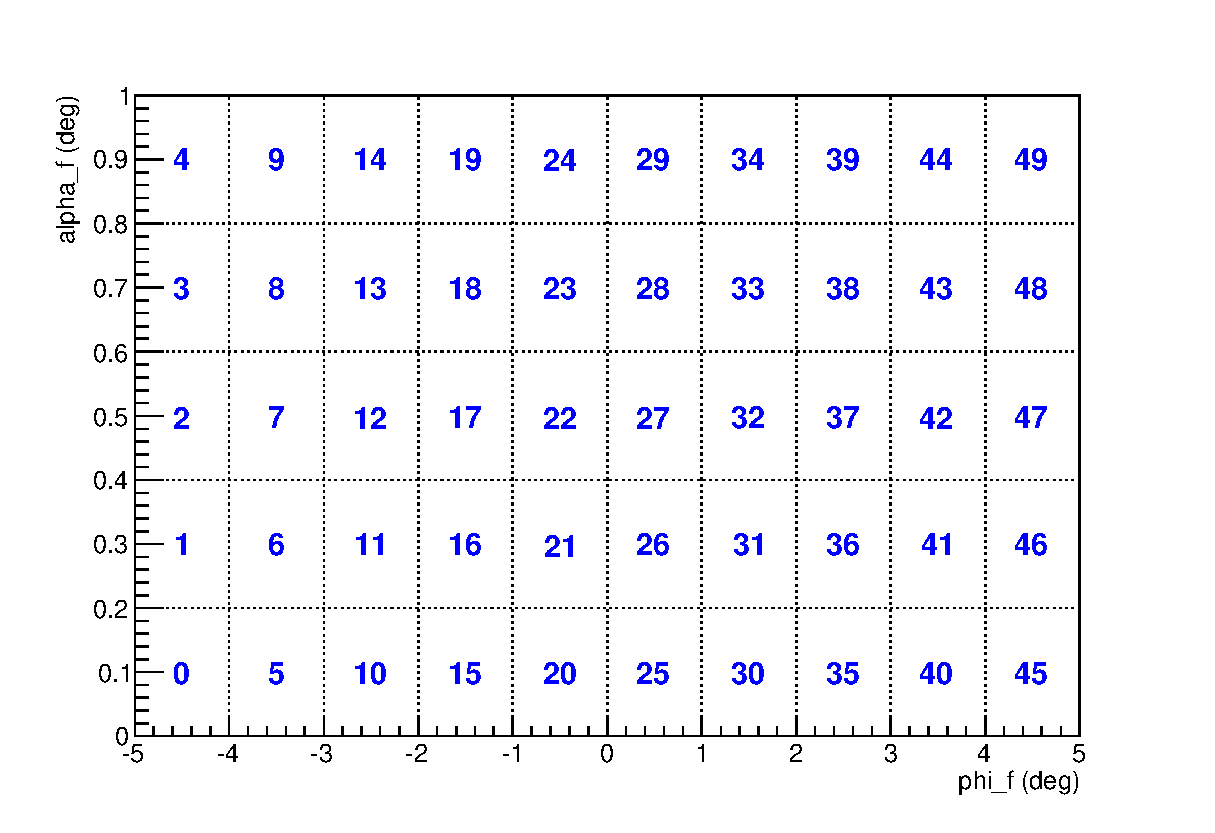
\includegraphics[clip=, width=120mm]{fig/drawing/UserAPI_IntensityDataLayout.eps}
  \caption{The axes layout of IntensityData object.}
  \label{fig:UserApi:IntensityData}
\end{figure}

The x-axis and y-axis of the figure correspond to the $\phi_f$ and $\alpha_f$ axes of the detector.
The x-axis is divided into 10 bins,
with low edge of the first bin set to $-5.0\,{\rm deg}$ and upper edge of the last bin set to $+5.0\,{\rm deg}$.
The y-axis is divided into 5 bins,
with low edge of the first bin set to $0.0\,{\rm deg}$ and upper edge of the last bin set to $1.0\,{\rm deg}$.
There are 50 bins in total (they are marked on the plot with indexes from 0 to 49), each bin will contain one intensity value.

During a standard simulation (i.e. no Monte-Carlo integration involved) intensities are calculated for $\phi_f, \alpha_f$ values corresponding to the bin centers, e.g. the intensity stored in bin\#42 will correspond to $\phi_f=3.5\,{\rm deg}, \alpha_f=0.5\,{\rm deg}$.
\vspace*{2mm}


\Note{
The \Code{IntensityData} object is not intended for direct usage from Python API. The idea is
that the API provides the user with the possibility to export the data from BornAgain internal format to the format of his choice as well as import user's data into BornAgain.
For the moment this functionality is limited to a few options explained below.
We encourage users feedback to implement the support of most requested formats.}


\subsubsection{Import/export of intensity data}
For the moment we provide following options:
\begin{itemize}
\item Import/export of \Code{IntensityData} object from/to \Code{numpy} array.
\item Import/export of \Code{IntensityData} object from/to text file.

\end{itemize}

\paragraph{Export to numpy array}

To export intensity data into  \Code{numpy} array the method \Code{getArray()} should be used
on \Code{IntensityData} object as shown in line \ref{py:UserApi:getArray} of
following code snippet.

\begin{lstlisting}
intensity = simulation.getIntensityData()
array = intensity.getArray() @\label{py:UserApi:getArray}@
...
pylab.imshow(numpy.rot90(array, 1)) @\label{py:UserApi:imshow}@
pylab.show()
\end{lstlisting}

For the detector settings defined in the previous paragraph the dimensions of the resulting array will be (10,5). By using \Code{numpy} indexes the user can get access to the intensity values, e.g.
\Code{array[0][0]} corresponds to the intensity in bin\#0 of \cref{fig:UserApi:IntensityData},
\Code{array[0][4]} to bin\#4,
\Code{array[1][0]} to bin\#5,
\Code{array[8][2]} to bin\#42,
\Code{array[9][4]} to bin\#49.


To plot this resulting numpy array with \Code{matplotlib} it has to be rotated counter-clockwise
to match \Code{matplotlib} conventions as shown in line~\ref{py:UserApi:imshow}.


%\subsubsection{Direct access to the data}
%User can access to the

%\begin{lstlisting}[language=python, style=eclipseboxed]
%for i in range(0, intensity.getAllocatedSize()):
%    print intensity[i]
%\end{lstlisting}


\subsubsection{Importing from numpy array}

To use fitting the user has to load experimental data into BornAgain fitting kernel.
To read experimental data the user has to create
IntensityData object, fill it with the experimental  intensity values and pass
this object to the fitting kernel.

First, the user creates empty \Code{IntensityData} as shown
in line~\ref{py:UserApi:IntensityData} of the following code snippet.
\begin{lstlisting}
data = IntensityData() @\label{py:UserApi:IntensityData}@
data.addAxis(FixedBinAxis("phi_f", 10, -5.0*degree, 5.0*degree)) @\label{py:UserApi:phi_f}@
data.addAxis(FixedBinAxis("alpha_f", 5, 0.0*degree, 1.0*degree)) @\label{py:UserApi:alpha_f}@
...
array = numpy.zeros((10, 5)) # fill array with experimental intensities @\label{py:UserApi:create_array}@
...
data.setRawDataVector(array.flatten().tolist()) @\label{py:UserApi:set_raw}@

fitSuite = FitSuite() @\label{py:UserApi:fit_suite}@
fitSuite.addSimulationAndRealData(simulation, data) @\label{py:UserApi:add_real_data}@
\end{lstlisting}

In lines~\ref{py:UserApi:phi_f}, \ref{py:UserApi:alpha_f} two axes with fixed bin sizes
are defined to represent the detector layout as shown in \cref{fig:UserApi:IntensityData}.
The constructor of \Code{FixedBinAxis} object has the following signature

\begin{lstlisting}
FixedBinAxis(title, nbins, min_angle, max_angle)
\end{lstlisting}

The created \Code{IntensityData} object has to be filled with experimental intensities
using \Code{numpy} array prepared by the user (lines ~\ref{py:UserApi:create_array}-~\ref{py:UserApi:set_raw}). In lines \ref{py:UserApi:fit_suite},\ref{py:UserApi:add_real_data} the fitting kernel is created and initialized with \Code{Simulation} object and
\Code{IntensityData} object representing the experimental data.


\subsubsection{Saving intensity data to text file.}

The special class \Code{IntensityDataIOFactory} is intended for saving the intensity data
in different datafile formats. For the moment, it only supports saving the data in specific BornAgain's text files (the file extention \Code{*.int}).

\begin{lstlisting}
intensity = simulation.getIntensityData()
IntensityDataIOFactory.writeIntensityData(intensity, 'file_name.int')
\end{lstlisting}

\subsubsection{Reading intensity data from a text file.}
The same class is also intended for reading intensity data
from files with different formats. For the moment, it only supports reading the data from text files of special BornAgain's format (the file extention \Code{*.int}).

\begin{lstlisting}
intensity = IntensityDataIOFactory.readIntensityData('file_name.int')
\end{lstlisting}
\fi

%%%%%%%%%%%%%%%%%%%%%%%%%%%%%%%%%%%%%%%%%%%%%%%%%%%%%%%%%%%%%%%%%%%%%%%%%%%%%%%%
%%
%%   BornAgain User Manual
%%
%%   homepage:   http://www.bornagainproject.org
%%
%%   copyright:  Forschungszentrum Jülich GmbH 2015
%%
%%   license:    Creative Commons CC-BY-SA
%%
%%   authors:    Scientific Computing Group at MLZ Garching
%%               C. Durniak, M. Ganeva, G. Pospelov, W. Van Herck, J. Wuttke
%%
%%%%%%%%%%%%%%%%%%%%%%%%%%%%%%%%%%%%%%%%%%%%%%%%%%%%%%%%%%%%%%%%%%%%%%%%%%%%%%%%

\chapter{Sample}\label{SRefSam}

%%%%%%%%%%%%%%%%%%%%%%%%%%%%%%%%%%%%%%%%%%%%%%%%%%%%%%%%%%%%%%%%%%%%%%%%%%%%%%%%
\section{Multilayer}\label{SRefMuLay}
%%%%%%%%%%%%%%%%%%%%%%%%%%%%%%%%%%%%%%%%%%%%%%%%%%%%%%%%%%%%%%%%%%%%%%%%%%%%%%%%

Samples in BornAgain are always of type \ttIdx{MultiLayer}.

\setCpp
\begin{lstlisting}
class MultiLayer {
    MultiLayer();
    void addLayer(const Layer& p_child);
    void addLayerWithTopRoughness(const Layer& layer, const LayerRoughness& roughness);
};
\end{lstlisting}

A \texttt{MultiLayer} consists of one or more layers,
numbered from top to bottom as shown in~\cref{Fdefz}.
The function \clFct{MultiLayer}{addLayer} or \clFct{MultiLayer}{addLayerWithTopRoughness}
inserts one \ttIdx{Layer} at the high-index, low-$z$ end.

The \texttt{Layer} API is documented in~\cref{SRefLayer},
the \ttIdx{LayerRoughness} in~\cref{SRefRough}.

The following Python code fragment constructs an absolutely minimal sample:

\setPy
\begin{lstlisting}
sample = MultiLayer()
sample.addLayer(air_layer)
\end{lstlisting}

This sample just consists of an infinite volume of air.
As such, it is completely inert; it causes neither refraction, nor scattering.
However, the air layer can be \E{decorated} with a \ttIdx{ParticleLayout},
which then causes small-angle scattering,
as demostrated in the tutorial \tuto{51}{Cylinders in Born Approximation}.

The following sample consists of two half-infinite layers,
substrate under air:

\setPy
\begin{lstlisting}
sample = MultiLayer()
sample.addLayer(air_layer)
sample.addLayer(substrate_layer)
\end{lstlisting}

%%%%%%%%%%%%%%%%%%%%%%%%%%%%%%%%%%%%%%%%%%%%%%%%%%%%%%%%%%%%%%%%%%%%%%%%%%%%%%%%
\section{Layer}\label{SRefLayer}
%%%%%%%%%%%%%%%%%%%%%%%%%%%%%%%%%%%%%%%%%%%%%%%%%%%%%%%%%%%%%%%%%%%%%%%%%%%%%%%%

A \ttIdx{Layer} is constructed through the following API:

\setCpp
\begin{lstlisting}
class Layer {
    Layer();
    Layer(const IMaterial& material, double thickness=0);
    void setThickness(double thickness);
    void setMaterial(const IMaterial& material);
    void addLayout(const ParticleLayout& decoration);
};
\end{lstlisting}

It is obligatory to set a \E{material} (\cref{SRefMat}).

The \E{thickness} must be nonnegative.
The semi-infinite top and bottom layer must have a \E{pro forma} thickness of~0.
All other layers should have a thickness larger than~0.

The \texttt{Layer} can be \E{decorated} with any number of \ttIdx{ParticleLayout}s.\footnote
{The source code only requires the particle decoration to be of type \ttIdx{ILayout}.
However, since this interface is realized by no other class besides \ttIdx{ParticleLayout},
we here spell out \texttt{ILayout} as \texttt{ParticleLayout}.}
Scattering from different layouts adds incoherently.

%%%%%%%%%%%%%%%%%%%%%%%%%%%%%%%%%%%%%%%%%%%%%%%%%%%%%%%%%%%%%%%%%%%%%%%%%%%%%%%%
\section{Material}\label{SRefMat}
%%%%%%%%%%%%%%%%%%%%%%%%%%%%%%%%%%%%%%%%%%%%%%%%%%%%%%%%%%%%%%%%%%%%%%%%%%%%%%%%

Material classes all inherit from the pure virtual interface class \ttIdx{IMaterial}.
Currently, BornAgain only supports homogeneous materials.
They can be either nonmagnetic or magnetic.
A nonmagnetic \ttIdx{HomogeneousMaterial} is created through the API

\setCpp
\begin{lstlisting}
class HomogeneousMaterial {
    HomogeneousMaterial(const std::string &name, const complex_t refractive_index);
    HomogeneousMaterial(const std::string &name, double refractive_index_delta, double refractive_index_beta);
};
\end{lstlisting}

The second form of the constructor computes the complex refractive index
\index{Refractive index!HomogeneousMaterial@\Code{HomogeneousMaterial}}%
from the two real parameters $\delta$ and~$\beta$ according to~\cref{Endb1}.

Typical usage is:

\setPy
\begin{lstlisting}
m_air = HomogeneousMaterial("Air", 0.0, 0.0)
m_substrate = HomogeneousMaterial("Substrate", 6e-6, 2e-8)
m_particle = HomogeneousMaterial("Particle", 6e-4, 2e-8)
\end{lstlisting}

A \ttIdx{HomogeneousMagneticMaterial} has the \E{magnetic field} (in units of Tesla)
\index{Magnetic field}%
as additional parameter:

\setCpp
\begin{lstlisting}
class HomogeneousMagneticMaterial {
    HomogeneousMagneticMaterial(const std::string &name, const complex_t refractive_index, const kvector_t magnetic_field);
    HomogeneousMagneticMaterial(const std::string &name, double refractive_index_delta, double refractive_index_beta, const kvector_t magnetic_field);
    void setMagneticField(const kvector_t magnetic_field);
}
\end{lstlisting}

%%%%%%%%%%%%%%%%%%%%%%%%%%%%%%%%%%%%%%%%%%%%%%%%%%%%%%%%%%%%%%%%%%%%%%%%%%%%%%%%
\section{Roughness}\label{SRefRough}
%%%%%%%%%%%%%%%%%%%%%%%%%%%%%%%%%%%%%%%%%%%%%%%%%%%%%%%%%%%%%%%%%%%%%%%%%%%%%%%%

\MissingSection

%%%%%%%%%%%%%%%%%%%%%%%%%%%%%%%%%%%%%%%%%%%%%%%%%%%%%%%%%%%%%%%%%%%%%%%%%%%%%%%%
%%
%%   BornAgain User Manual
%%
%%   homepage:   http://www.bornagainproject.org
%%
%%   copyright:  Forschungszentrum Jülich GmbH 2015
%%
%%   license:    Creative Commons CC-BY-SA
%%
%%   authors:    Scientific Computing Group at MLZ Garching
%%               C. Durniak, M. Ganeva, G. Pospelov, W. Van Herck, J. Wuttke
%%
%%%%%%%%%%%%%%%%%%%%%%%%%%%%%%%%%%%%%%%%%%%%%%%%%%%%%%%%%%%%%%%%%%%%%%%%%%%%%%%%

\chapter{Embedded particles}\label{SRefParticles}

%%%%%%%%%%%%%%%%%%%%%%%%%%%%%%%%%%%%%%%%%%%%%%%%%%%%%%%%%%%%%%%%%%%%%%%%%%%%%%%%
\section{Particle layout}\label{SRefPLay}
%%%%%%%%%%%%%%%%%%%%%%%%%%%%%%%%%%%%%%%%%%%%%%%%%%%%%%%%%%%%%%%%%%%%%%%%%%%%%%%%

A \ttIdx{ParticleLayout} is constructed through the following API:

\setCpp
\begin{lstlisting}
class ParticleLayout {
    ParticleLayout();
    ParticleLayout(const IAbstractParticle& particle);
    ParticleLayout(const IAbstractParticle& particle, double abundance);
    void addParticle(const IAbstractParticle& particle);
    void addParticle(const IAbstractParticle& particle, double abundance);
    void addParticle(const IParticle& particle, double abundance, const kvector_t position);
    void addParticle(const IParticle& particle, double abundance, const kvector_t position, const IRotation& rotation);
    void addInterferenceFunction(const IInterferenceFunction& interference_function);
    void setTotalParticleSurfaceDensity(double particle_density);
};
\end{lstlisting}

An \ttIdx{IAbstractParticle} is either an \ttIdx{IParticle} (\cref{SRefIPart})
or a \ttIdx{Particle\-Distri\-bution} (\cref{SRefPDis}).
\index{Particle!IAbstractParticle@\Code{IAbstractParticle}}%
\index{Particle!IParticle@\Code{IParticle}}%
\index{Particle!ParticleDistribution@\Code{ParticleDistribution}}%
In any case, it does not stand for \E{one} particle,
but for one kind of particles.
A \texttt{ParticleLayout} can be loaded with any number of \texttt{IAbstractParticle}s,
using the function \clFct{IAbstractParticle}{addParticle}.

Most often, a \texttt{ParticleLayout} is to be loaded with just one \texttt{IAbstractParticle}.
In this case, \texttt{IAbstractParticle} can be passed as an argument of the
\texttt{ParticleLayout} constructor,
and no call of \texttt{addParticle} is needed;
by default, the \texttt{abundance} is set to~1.
\index{Abundance}%
If there are several \texttt{IAbstractParticle}s,
then the parameter \texttt{abundance} of the function \texttt{addParticle} must be used for
a number that expresses the relative number density of the particle kind.

\Work{Explain \texttt{position} and \ttIdx{IRotation} \ldots}

%%%%%%%%%%%%%%%%%%%%%%%%%%%%%%%%%%%%%%%%%%%%%%%%%%%%%%%%%%%%%%%%%%%%%%%%%%%%%%%%
\section{IParticle}\label{SRefIPart}
%%%%%%%%%%%%%%%%%%%%%%%%%%%%%%%%%%%%%%%%%%%%%%%%%%%%%%%%%%%%%%%%%%%%%%%%%%%%%%%%

\MissingSection

%%%%%%%%%%%%%%%%%%%%%%%%%%%%%%%%%%%%%%%%%%%%%%%%%%%%%%%%%%%%%%%%%%%%%%%%%%%%%%%%
\section{Particle distribution}\label{SRefPDis}
%%%%%%%%%%%%%%%%%%%%%%%%%%%%%%%%%%%%%%%%%%%%%%%%%%%%%%%%%%%%%%%%%%%%%%%%%%%%%%%%

\MissingSection

%%%%%%%%%%%%%%%%%%%%%%%%%%%%%%%%%%%%%%%%%%%%%%%%%%%%%%%%%%%%%%%%%%%%%%%%%%%%%%%%
%%
%%   BornAgain User Manual
%%
%%   homepage:   http://www.bornagainproject.org
%%
%%   copyright:  Forschungszentrum Jülich GmbH 2015
%%
%%   license:    Creative Commons CC-BY-SA
%%
%%   authors:    Scientific Computing Group at MLZ Garching
%%               C. Durniak, M. Ganeva, G. Pospelov, W. Van Herck, J. Wuttke
%%
%%%%%%%%%%%%%%%%%%%%%%%%%%%%%%%%%%%%%%%%%%%%%%%%%%%%%%%%%%%%%%%%%%%%%%%%%%%%%%%%

\def\ffsection#1{%
\FloatBarrier\clearpage
\section{#1}}

\def\ffref#1{\texttt{#1} (\cref{S#1})}

% Don't number subfigures in this chapter.
\makeatletter
\renewcommand{\@thesubfigure}{\relax}
\makeatother

\index{Cone|see{Frustum}}
\index{Cuboid|see{Box}}
\index{Expansion|see{Cantellation}}
\index{Prism!reactangular|see{Box}}
\index{Tilt|see{Rotation}}
\index{Truncation|seealso{Facetting}}
\index{Truncation!cone|see{Frustum}}
\index{Truncation!pyramid|see{Frustum}}

%%%%%%%%%%%%%%%%%%%%%%%%%%%%%%%%%%%%%%%%%%%%%%%%%%%%%%%%%%%%%%%%%%%%%%%%%%%%%%%%
\chapter{Introduction}\label{SPFF}
%%%%%%%%%%%%%%%%%%%%%%%%%%%%%%%%%%%%%%%%%%%%%%%%%%%%%%%%%%%%%%%%%%%%%%%%%%%%%%%%

BornAgain comes with a comprehensive collection of hard-coded shape transforms
\index{Shape transform}%
for standard particle geometries like
spheres, cylinders, prisms, pyramids or ripples.
This collection is documented in the following.
For each shape,
the real-space geometry is shown in orthogonal projections,
the parameters of the BornAgain method are defined,
an analytical expression for the form factor is given,
and exemplary results for $\left|F(\q)\right|^2$ versus
$\alpha_\sf,\phi_\sf$ are shown for small-angle scattering conditions
($\alpha_\si=\phi_\si=0$).

The computation of $F(\q)$ is based on
shapes $S(\r)$ given in Cartesian coordinates,
as defined in the orthogonal projections.
Typically, the vertical ($z$) direction is chosen
along a symmetry axis of the particle.
The origin is always at the center of the bottom side of the particle.
Different parametrization or a different choice of the origin
cause our analytic form factors to trivially deviate
from expressions given in the \IsGISAXS\ manual \cite[Sec.~2.3]{Laz06}
or in the literature \cite[Appendix]{ReLL09}.

We made sure that all expressions also hold for complex scattering vectors ~$\q$,
\index{q@$q$ (scattering vector)}%
\index{Scattering vector}%
used to describe in order to take any material absorption into account.
\index{Absorption}%
In standard reflectometry geometry, with reference surface normal to $\v{\hat z}$,
\index{z@$z$ (surface normal coordinate)}%
\index{Coordinates}%
\index{Surface}%
only the vertical components of $\k_\si$ and $\k_\sf$ can have imaginary parts.
However,
for tilted particles
$F(\v{\tilde{q}})$ needs to be computed with
a rotated scattering vector~$\v{\tilde q}$
that may be complex in all three components.
Therefore BornAgain allows all three components of~$\q$ to be complex.

In the following,
information about the implemented geometries is given in standardized form.
Analytical expressions are given for the form factor $F(\q)$,
for the volume $V=F(0)$,
\index{Volume}%
and for the maximum horizontal section $S$
(the area of the particle as seen from above).
Mathematical notation in the form factor expressions includes
the cardinal sine functions $\sinc(z)\coloneqq\sin(z)/z$
\index{sinc (sinus cardinalis)}%
and the Bessel function of first kind and first order $J_1(z)$
\index{J@$J_1$ (Bessel function)}%
\index{Bessel function}%
\cite[Ch.~9]{AbSt64}.
If results contain an integral,
then no analytical form was found,
and the integral is evaluated by numeric quadrature.
\index{Quadrature}%
For polyhedral figures,
\index{Polyhedron!generic algorithm}%
except a few simple ones like the rectangular box,
we use a generic form factor computation,
parametrized by the vertices of the figure,
that is described in full detail in a mathematical paper~\cite{Wut17}.

Almost all analytical expressions for $F(\q)$ contain
removable singularities for certain values of $\q$.
Our implementation uses proper analytic continuations at these singularities,
\index{Singularity!in form factor computation}%
though this is not explicitly denoted in the following formula collection.
Furthermore, series expansions are used to ensure numeric accuracies
in the neighborhood of the singularities.
For polyhedra, see Ref.~\cite{Wut17} for a meticulous discussion.

\begin{figure}[t]
\begin{center}
\includefinal{1\TW}{fig/ff2/ff_demo_1quadrants.pdf}
\end{center}
\caption{Normalized intensity $I(\alpha_\sf,\phi_\sf)$
for small-angle scattering by a truncated sphere with $R=4.2$~nm and $H=6.1$~nm,
for four different tilt angles~$\vartheta$ (rotation around the $y$ axis).
Since $I$ possess the standard symmetry (\protect\ref{EFq4sym}),
data are only shown for first quadrant $0^\circ\le\phi_\sf,\alpha_\sf\le 5^\circ$.}
\label{F1quadrants}
\end{figure}

Geometrical objects can be parametrized in different ways.
Concerns about user experience and about code readability
sometimes lead to different choices.
For the BornAgain user interfaces (GUI and API)
we have chosen the most standard parameters,
as used in elementary geometry, like length, height, radius,
even if this is at variance from the \IsGISAXS\ precedent.
Where our parametrization made analytic expressions too tedious,
we use alternate internal parameters to alleviate the formul\ae.

Examplary form factors are numerically computed in Born approximation.
All simulations scripts can be found in the BornAgain sources in directory
\href{https://github.com/scgmlz/BornAgain/tree/master/Doc/FFCatalog/fig/ff2}%
{Doc/FFCatalog/fig/ff2}.
The particles are assigned a refractive index of $n=10^{-5}$.
\index{Refractive index}%
Parameters are chosen such that
the particle volume~$V$
\index{Volume}%
is about 250~nm$^3$ (within $\pm5$~\%);
except ripples, which are chosen with a vertical section $V/L$ of 40~nm$^2$
and a length of 25~nm.
The incident wavelength is 1~\AA.
The incident beam is always in $x$ direction, hence $\alpha_\si=\phi_\si=0$.
Simulated detector images are normalized to the maximum scattering intensity at $F(0)=V$,
\begin{equation}
  I(\alpha_\sf,\phi_\sf)\coloneqq |F(q(\alpha_\sf,\phi_\sf))|^2/V^2.
\end{equation}
All plots
\index{Plotting}%
have the same logarithmic color scale,
extending over eight decades from $10^{-8}$ to~1.
Plot ranges in $\alpha_\sf$ and $\phi_\sf$ are also standardized as far as
reasonably possible.
For some geometries,
the simulated detector image has some symmetry,
\index{Symmetry}
namely horizontal or/and vertical mirror planes:
\index{Mirror planes}
\begin{equation}\label{EFq4sym}
  I(\alpha_\sf,\phi_\sf)
  = I(\alpha_\sf,-\phi_\sf)
  = I(-\alpha_\sf,-\phi_\sf)
  = I(\alpha_\sf,-\phi_\sf).
\end{equation}
% TODO RESTORE TEMPORARILY REMOVED XREF
% The physical origin this symmetry is discussed in \cref{Ssym}.
In these cases, we tend to restrict
plots of $I$ to the quadrant $\alpha_\sf\ge0$, $\phi_\sf\ge0$.
However, it requires some experience to fully appreciate the
information content of these plots.
For a demonstration of this,
try to grasp the main features of \cref{F1quadrants}.
Then compare with \cref{F4quadrants}.

\begin{figure}[t]
\begin{center}
\includefinal{1\TW}{fig/ff2/ff_demo_4quadrants.pdf}
\end{center}
\caption{Same data as in Fig.~\protect\ref{F1quadrants},
but now shown for all four quadrants ($-5^\circ\le\phi_\sf,\alpha_\sf\le 5^\circ$).
The vertical interference pattern,
which gradually disappears with increasing tilt angle,
 is much more salient in this plot
than in the preceding one-quadrant representation.}
\label{F4quadrants}
\end{figure}

\index{Large particles!numeric difficulty}%
\index{Numeric difficulty!form factor oscillation}%
\index{Oscillation!from large particle form factor}%
\index{Monte-Carlo integration!for large particle form factor}%
\index{Particle!rapid form factor oscillation}%
Finally, one warning: For large particles (typically of order 1000~nm),
  the form factor oscillates rapidly within one detector bin
  so that analytical calculations (performed for the bin center)
  may give a completely wrong intensity pattern.
Several ways to work around this problem are proposed in Sect.~5.3
of our reference paper~\cite{PoHB20}.

%%%%%%%%%%%%%%%%%%%%%%%%%%%%%%%%%%%%%%%%%%%%%%%%%%%%%%%%%%%%%%%%%%%%%%%%%%%%%%%%
\chapter{Hard particles}\label{SHPFF}
%%%%%%%%%%%%%%%%%%%%%%%%%%%%%%%%%%%%%%%%%%%%%%%%%%%%%%%%%%%%%%%%%%%%%%%%%%%%%%%%
\index{Particle!hard|(}

The following tables summarize the implemented particle geometries,
 roughly ordered by decreasing symmetry.
Afterwards, the detailed documentation is in alphabetical order.

%\clearpage\thispagestyle{empty}
\def\figuredentry#1#2#3#4#5#6{%
 #2 &
 \texttt{#1}& %\newline\textsl{#1} &
#5 & % symmetry
#4 & % parameters
Page~\pageref{S#3}\\} % , \cref{S#3}
\def\sizedentry#1#2#3#4#5{\figuredentry{#1}{\hspace{#5ex}\raisebox{#4ex}{\includefinal{#3em}{fig/blue/#2.png}}}}
\def\entry#1#2{\sizedentry{#1}{#2}{5}{-3.8}{0}}
\begin{center}
  \def\h{\text{h}}
  \def\v{\text{v}}
\small
\begin{longtable}
  {@{}p{.14\textwidth}
   @{}p{.32\textwidth}
   @{}p{.17\textwidth}
   @{}p{.19\textwidth}
   @{}p{.15\textwidth}@{}}
% Shape&{Name\newline \textsl{Legacy Name}}&Symmetry&Parameters&Reference\\\hline
Shape&Name&Symmetry&Parameters&Reference\\\hline\\[-2ex]
\sizedentry{Dot}{Dot3d}{2}{-2}{2}{Dot}{$R_\text{scat}$}{R$_3$}{Dot}
\entry{FullSphere}{FullSphere3d}{FullSphere}{$R$}{R$_3$}{Sphere}
\entry{FullSpheroid}{FullSpheroid3d}{FullSpheroid}{$R$, $H$}{D$_{\infty\h}$}{Spheroid}
\entry{Cylinder}{Cylinder3d}{Cylinder}{$R$, $H$}{D$_{\infty\h}$}{Cylinder}
\entry{TruncatedSphere}{Sphere3d}{TruncatedSphere}{$R$, $H$}{C$_{\infty\v}$}{SphericalCap}
\entry{TruncatedSpheroid}{Spheroid3d}{TruncatedSpheroid}{$R$, $H$, $f_p$}{C$_{\infty\v}$}{SpheroidalCap}
\entry{Cone}{Cone3d}{Cone}{$R$, $H$, $\alpha$}{C$_{\infty\v}$}{ConicalFrustum}
\entry{Icosahedron}{Icosahedron3d}{Icosahedron}{$L$}{I$_\h$}{Icosahedron}
\entry{Dodecahedron}{Dodecahedron3d}{Dodecahedron}{$L$}{I$_\h$}{Dodecahedron}
\entry{TruncatedCube}{TruncatedCube}{TruncatedCube}{$L$, $t$}{O$_\h$}{TruncatedCube}
\sizedentry{CantellatedCube}{Box3d}{0.1}{0}{0}%TODO
{CantellatedCube}{$L$, $t$}{O$_\h$}{CantellatedCube}
\entry{Prism6}{Prism63d}{Prism6}{$R$, $H$}{D$_{6\h}$}{Prism6}
\entry{Cone6}{Cone63d}{Cone6}{$R$, $H$, $\alpha$}{C$_{6\v}$}{Frustum6}
\entry{Pyramid}{Pyramid3d}{Pyramid}{$L$, $H$, $\alpha$}{C$_{4\v}$}{Frustum4}
\entry{Cuboctahedron}{Cuboctahedron3d}{Cuboctahedron}{$L$, $H$, $r_H$, $\alpha$}{C$_{4\v}$}{BiFrustum4}
\entry{Prism3}{Prism33d}{Prism3}{$L$, $H$}{D$_{3\h}$}{Prism3}
\entry{Tetrahedron}{Tetrahedron3d}{Tetrahedron}{$L$, $H$, $\alpha$}{C$_{3\v}$}{Frustum3}
\entry{EllipsoidalCylinder}{EllipsoidalCylinder3d}{EllipsoidalCylinder}{$R_a$, $R_b$, $H$}{D$_{2\h}$}{EllipsoidalCylinder}
\entry{Box}{Box3d}{Box}{$L$, $W$, $H$}{D$_{2\h}$}{Prism2}
\entry{HemiEllipsoid}{HemiEllipsoid3d}{HemiEllipsoid}{$R_a$, $R_b$, $H$}{C$_{2\v}$}{HemiEllipsoid}
\entry{AnisoPyramid}{AnistropicPyramid3d}{AnisoPyramid}{$L$, $W$, $H$, $\alpha$}{C$_{2\v}$}{Frustum2}
\hline
\end{longtable}
\end{center}
%\thispagestyle{empty}\clearpage

\index{Rotation of particles}
\index{Orientation of particles}
\index{CreateRotateX@\Code{CreateRotateX}}
\index{Transform3D@\Code{Transform3D}}

%===============================================================================
\ffsection{AnisoPyramid (rectangle-based)} \label{SAnisoPyramid}
%===============================================================================
\index{Frustum!reactangular base}
\index{Anisotropic pyramid}
\index{Pyramid!rectangular}
\index{FormFactorAnisoPyramid@\Code{FormFactorAnisoPyramid}}

\paragraph{Real-space geometry}\strut\\

\begin{figure}[H]
\hfill
\subfigure[Perspective]{\includefinal{.24\TW}{fig/blue/AnistropicPyramid3d.png}}
\hfill
\subfigure[Top view]{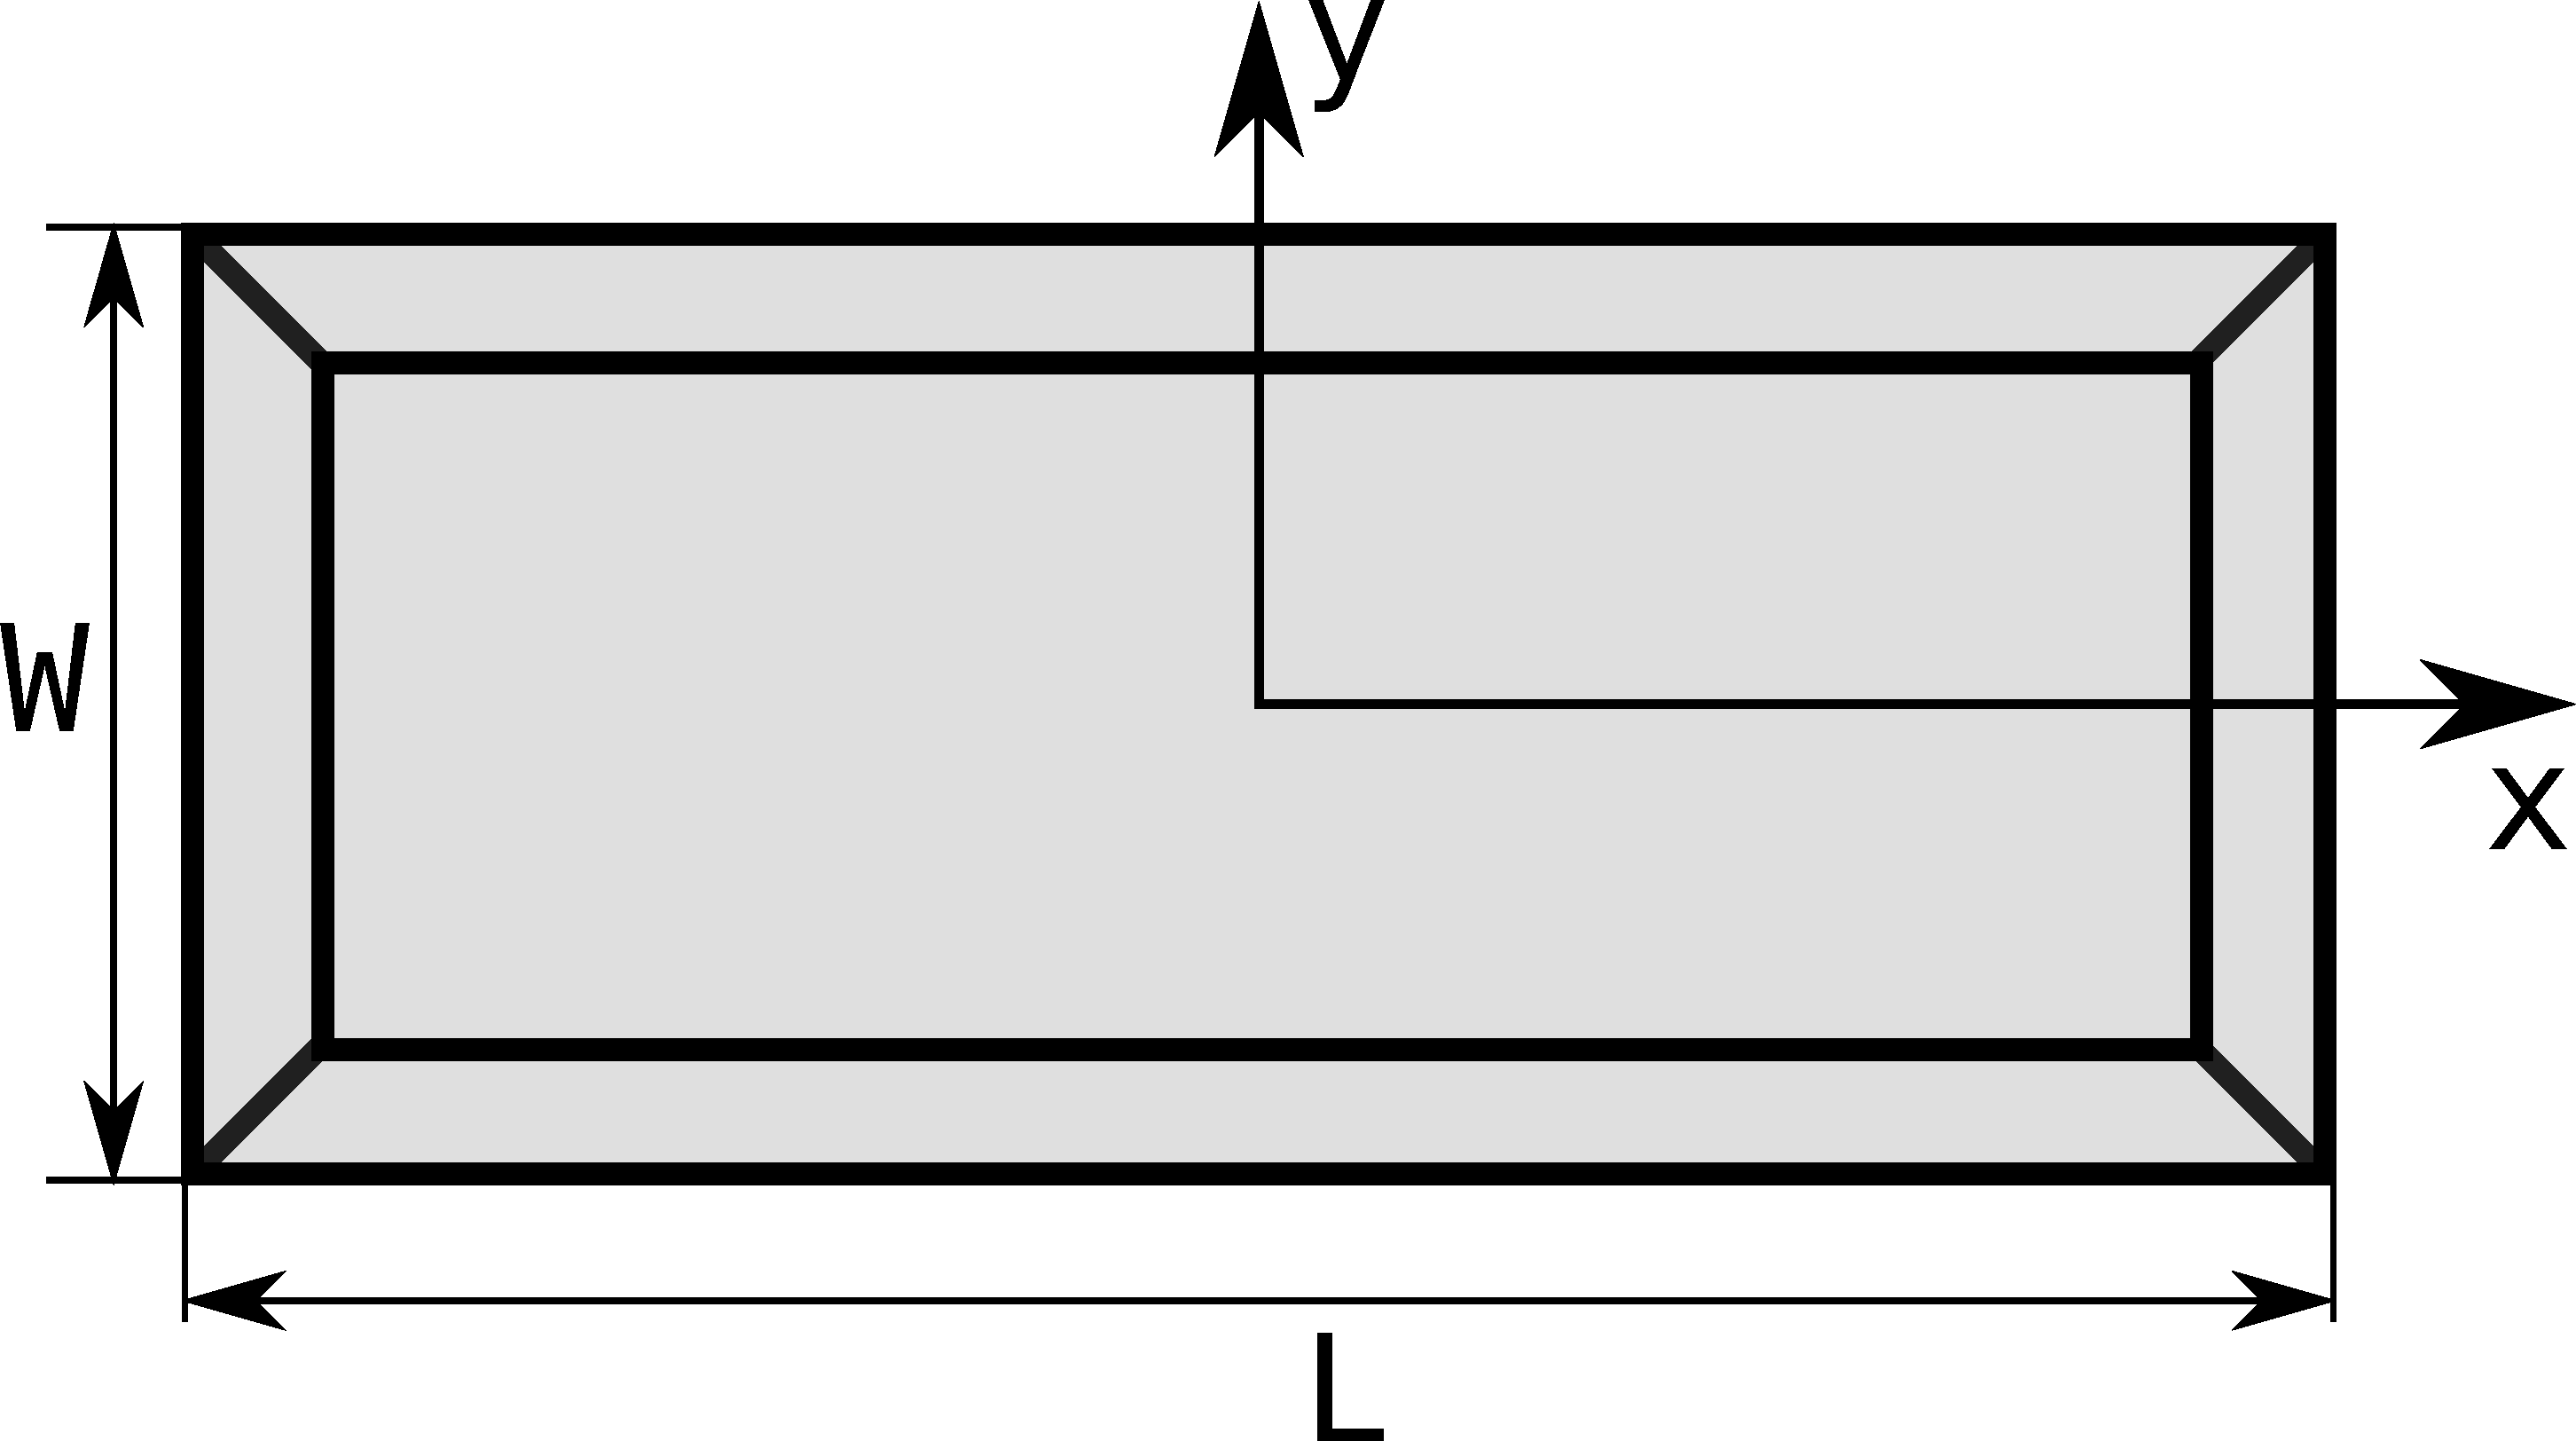
\includegraphics[width=.30\textwidth]{fig/cuts/AnisoPyramid2dxy.pdf}}
\hfill
\subfigure[Side view]{\raisebox{2mm}{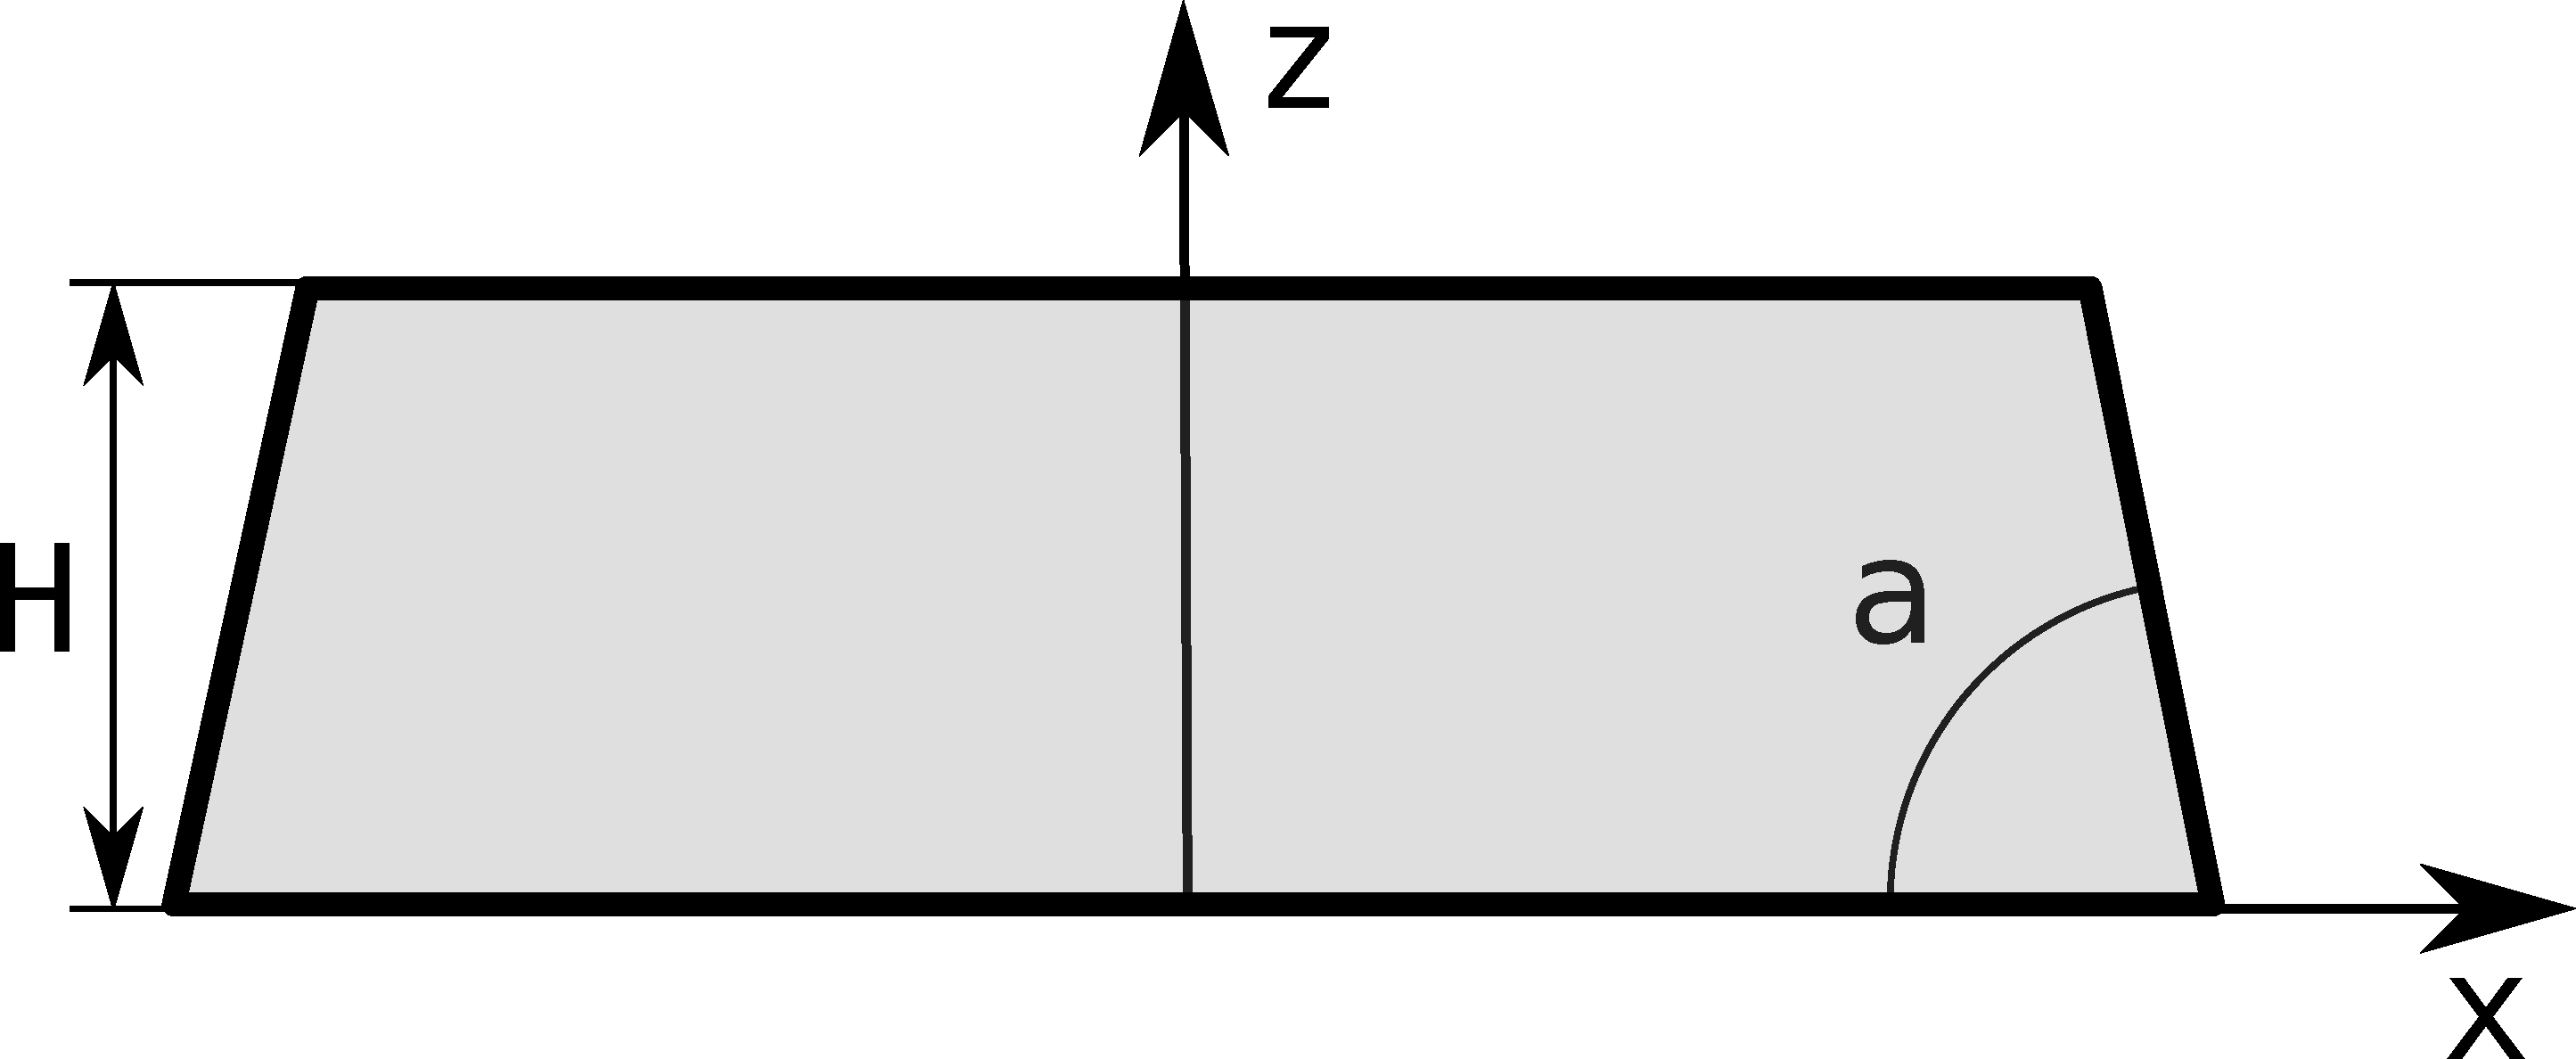
\includegraphics[width=.30\textwidth]{fig/cuts/AnisoPyramid2dxz.pdf}}}
\hfill
\caption{A truncated pyramid with a rectangular base.}
\end{figure}

\FloatBarrier

\paragraph{Syntax and parameters}\strut\\[-2ex plus .2ex minus .2ex]
\begin{lstlisting}
  FormFactorAnisoPyramid(double length, double width, double height, double alpha)
\end{lstlisting}
with the parameters
\begin{itemize}
\item \texttt{length} of the base, $L$,
\item \texttt{width} of the base, $W$,
\item \texttt{height}, $H$
\item \texttt{alpha}, angle between the base and a side face, $\alpha$.
\end{itemize}
They must fulfill
\begin{displaymath}
  H \le \frac{\tan\alpha}{2} \min\,(L,W).
\end{displaymath}

\paragraph{Form factor, volume, horizontal section}\strut\\
\begin{equation*}
  F \text{~: computed using the generic polyhedron form factor~\cite{Wut17},}
\end{equation*}
\begin{equation*}
  V= H \Big[LW - \dfrac{(L + W)H}{\tan\alpha} + \dfrac{4}{3} \dfrac{H^2}{\tan^2\alpha}\Big].
\end{equation*}
\begin{equation*}
  S=LW.
\end{equation*}

\paragraph{Examples}\strut\\
\begin{figure}[H]
\begin{center}
\includefinal{1\TW}{fig/ff2/ff_AnisoPyramid.pdf}
\end{center}
\caption{Normalized intensity $|F|^2/V^2$,
computed with $L=13$~nm, $W=8$~nm, $H=4.2$~nm, and $\alpha=60^\circ$,
for four different angles~$\omega$ of rotation around the $z$ axis.}
\label{fig:FFAnisoPyramidEx}
\end{figure}

\paragraph{History}\strut\\
Agrees with the \E{In-plane anisotropic pyramid} form factor of \IsGISAXS\
\cite[Eq.~2.40]{Laz06} \cite[Eq.~217]{ReLL09},
except for different parametrization.
This is \E{not} the \E{anisotropic pyramid} of \FitGISAXS,
which is a true pyramid with an off-center apex \cite{Bab13}.

Formfactors~$F(\q)$ have been checked against the different computation of \IsGISAXS,
and were found to fully agree.

\paragraph{See also}
\begin{itemize}
\item \ffref{Box} if $\alpha=0$,
\item \ffref{Pyramid} if $L=W$.
\end{itemize}

%===============================================================================
\ffsection{Box (cuboid)} \label{SBox}
%===============================================================================
\index{Box}
\index{Cube}
\index{Platonic solid!cube}
\index{FormFactorBox@\Code{FormFactorBox}}

\paragraph{Real-space geometry}\strut\\

\begin{figure}[H]
\hfill
\subfigure[Perspective]{\includefinal{.24\TW}{fig/blue/Box3d.png}}
\hfill
\subfigure[Top view]{\includefinal{.3\TW}{fig/cuts/Box2dxy.pdf}}
\hfill
\subfigure[Side view]{\raisebox{2mm}{\includefinal{.3\TW}{fig/cuts/Box2dxz.pdf}}}
\hfill
\caption{A rectangular cuboid.}
\end{figure}

\FloatBarrier

\paragraph{Syntax and parameters}\strut\\[-2ex plus .2ex minus .2ex]
\begin{lstlisting}
  FormFactorBox(double length, double width, double height)
\end{lstlisting}
with the parameters
\begin{itemize}
\item \texttt{length} of the base, $L$,
\item \texttt{width} of the base, $W$,
\item \texttt{height}, $H$.
\end{itemize}

\paragraph{Form factor, volume, horizontal section}

\begin{equation*}
F= L W H\exp\left(i q_z \frac{H}{2}\right) \sinc\left(q_x \frac{L}{2}\right)
\sinc\left(q_y \frac{W}{2}\right) \sinc\left(q_z \frac{H}{2}\right),
\end{equation*}
\begin{equation*}
  V= LWH,
\end{equation*}
\begin{equation*}
  S = LW.
\end{equation*}

\paragraph{Examples}\strut

\begin{figure}[H]
\begin{center}
\includefinal{1\TW}{fig/ff2/ff_Box.pdf}
\end{center}
\caption{Normalized intensity $|F|^2/V^2$,
computed with $L=18$~nm, $W=4.6$~nm, and $H=3$~nm,
for four different angles~$\omega$ of rotation around the $z$ axis.}
\end{figure}

\paragraph{History}\strut\\
Agrees with \E{Box} form factor of \IsGISAXS\
\cite[Eq.~2.38]{Laz06} \cite[Eq.~214]{ReLL09},
except for factors $1/2$ in the definitions of parameters $L$, $W$, $H$.

\paragraph{See also}
\begin{itemize}
\item \ffref{AnisoPyramid} or \ffref{Pyramid}
  if sides are not vertical,
\item \ffref{TruncatedCube} if $L=W=H$ and corners are facetted,
\item \ffref{CantellatedCube} if $L=W=H$ and corners and edges are facetted,
\item Sect.~\ref{SBar} if elongated in one horizontal direction.
\end{itemize}

%===============================================================================
\ffsection{CantellatedCube} \label{SCantellatedCube}
%===============================================================================
\index{Cube!cantellated}
\index{Octahedron!cantellated}
\index{Cantellation!cube}
\index{FormFactorCantellatedCube@\Code{FormFactorCantellatedCube}}

\paragraph{Real-space geometry}\strut\\

% \begin{figure}[H]
% \hfill
% \subfigure[Perspective]{\includefinal{.24\TW}{fig/blue/CantellatedCube3d.png}}
% \hfill
% \subfigure[Top view]{\includefinal{.3\TW}{fig/cuts/Facettedcube2_2dxy.pdf}}
% \hfill
% \subfigure[Side view]{\includefinal{.3\TW}{fig/cuts/Facettedcube2_2dxz.pdf}}
% \hfill
% \caption{A cube whose eight vertices have been removed.
% The truncated part of each vertex is a trirectangular tetrahedron.}
% \end{figure}

A cube with truncated edges and vertices as in Fig~7 of Croset 2017 \cite{Cro17}.
Can also be obtained by cantellating an octahedron.
\FloatBarrier

\paragraph{Syntax and parameters}\strut\\[-2ex plus .2ex minus .2ex]
\begin{lstlisting}
  FormFactorCantellatedCube(double length, double removed_length)
\end{lstlisting}
with the parameters
\begin{itemize}
\item \texttt{length} of the full cube, $L$,
\item \texttt{removed\_length}, side length of the trirectangular tetrahedron removed from the cube's vertices, $t$.
\end{itemize}
They must fulfill
\begin{displaymath}
  t \le L/2.
\end{displaymath}

\paragraph{Form factor, volume, horizontal section}\strut\\
\begin{equation*}
  F \text{~: use the generic form factor of a polyhedron
             with inversion symmetry~\cite{Wut17},}
\end{equation*}
\begin{equation*}
  V = L^3 - 6 L t^2 + \frac{16}{3} t^3.
\end{equation*}
\begin{equation*}
  S = L^2.
\end{equation*}

\paragraph{Examples}\strut

% \begin{figure}[H]
% \begin{center}
% \includefinal{1\TW}{fig/ff2/ff_CantellatedCube.pdf}
% \end{center}
% \caption{Normalized intensity $|F|^2/V^2$,
% computed with $L=25$~nm, $W=10$~nm, $H=8$~nm, and $d=5$~nm,
% for four different angles~$\omega$ of rotation around the $z$ axis.}
% \end{figure}

\paragraph{History}\strut\\
Introduced in BornAgain--1.17 (Python only).
Motivated by Croset 2017 \cite{Cro17}.

\paragraph{See also}
\begin{itemize}
\item \ffref{Box} if $t=0$,
\item \ffref{TruncatedCube} if only the vertices are facetted.
\end{itemize}


%===============================================================================
\ffsection{Cone (circular)} \label{SCone}
%===============================================================================
\index{Frustum!circular base}
\index{FormFactorCone@\Code{FormFactorCone}}

\paragraph{Real-space geometry}\strut\\

\begin{figure}[H]
\hfill
\subfigure[Perspective]{\includefinal{.24\TW}{fig/blue/Cone3d.png}}
\hfill
\subfigure[Top view]{\includefinal{.3\TW}{fig/cuts/Cone2dxy.pdf}}
\hfill
\subfigure[Side view]{\raisebox{3mm}{\includefinal{.3\TW}{fig/cuts/Cone2dxz.pdf}}}
\hfill
\caption{A truncated cone with circular base.}
\end{figure}

\paragraph{Syntax and parameters}\strut\\[-2ex plus .2ex minus .2ex]
\begin{lstlisting}
  FormFactorCone(double radius, double height, double alpha)
\end{lstlisting}
with the parameters
\begin{itemize}
\item \texttt{radius}, $R$,
\item \texttt{height}, $H$,
\item \texttt{alpha}, angle between the side and the base, $\alpha$.
\end{itemize}
They must fulfill
\begin{displaymath}
  H\le R\tan\alpha.
\end{displaymath}

\paragraph{Form factor, volume, horizontal section}\strut\\
Notation:
\begin{equation*}
  R_H \coloneqq R-\dfrac{H}{\tan \alpha}, \quad
  q_{\parallel} \coloneqq \sqrt{q_x^2+ q_y^2}, \quad
  \tilde{q}_z \coloneqq q_z \tan\alpha.
\end{equation*}
Results:
\begin{equation*}
  F = 2\pi \tan\alpha\; \e^{i\tilde{q}_z R}
      \int_{R_H}^R \!\d\rho\, \rho^2
        \frac{J_1(q_{\parallel}\rho)}{q_{\parallel}\rho}\,\e^{-i\tilde{q}_z \rho},
\end{equation*}
\begin{equation*}
  V = \dfrac{\pi}{3}\tan\alpha  \left( R^3 - R_H^3\right),
\end{equation*}
\begin{equation*}
  S=\pi R^2.
\end{equation*}

\paragraph{Examples}\strut

\begin{figure}[H]
\begin{center}
\includefinal{1\TW}{fig/ff2/ff_Cone.pdf}
\end{center}
\caption{Normalized intensity $|F|^2/V^2$,
computed with $R=4$~nm, $H=11$~nm, and $\alpha=75^\circ$,
for four different tilt angles~$\vartheta$ (rotation around the $y$ axis).}
\end{figure}

\paragraph{History and Derivation}\strut\\
Agrees with \E{Cone} form factor of \IsGISAXS\
\cite[Eq.~2.28]{Laz06} \cite[Eq.~225]{ReLL09},
except for a substitution $z\to\rho$ in our expression for~$F$.
Justification for complex~$q$ in the same way as for the \E{Cylinder} form factor
in \cref{SCylinder}.

\paragraph{See also}
\begin{itemize}
\item \ffref{Cylinder} if $\alpha=0$.
\end{itemize}


%===============================================================================
\ffsection{Cone6 (hexagonal)} \label{SCone6}
%===============================================================================
\index{Frustum!hexagonal base}
\index{Pyramid!hexagonal}
\index{FormFactorCone6@\Code{FormFactorCone6}}

\paragraph{Real-space geometry}\strut\\

\begin{figure}[H]
\hfill
\subfigure[Perspective]{\includefinal{.24\TW}{fig/blue/Cone63d.png}}
\hfill
\subfigure[Top view]{\includefinal{.3\TW}{fig/cuts/Cone62dxy.pdf}}
\hfill
\subfigure[Side view]{\raisebox{5mm}{\includefinal{.3\TW}{fig/cuts/Cone62dxz.pdf}}}
\hfill
\caption{A truncated pyramid, based on a regular hexagon}
\end{figure}

\FloatBarrier
\paragraph{Syntax and parameters}\strut\\[-2ex plus .2ex minus .2ex]
\begin{lstlisting}
  FormFactorCone6(double base_edge, double height, double alpha)
\end{lstlisting}
with the parameters
\begin{itemize}
\item \texttt{base\_edge}, edge of the regular hexagonal base, $R$,
\item \texttt{height}, $H$,
\item \texttt{alpha}, dihedral angle between the base and a side face, $\alpha$.
\end{itemize}
Note that the orthographic projection does not show~$\alpha$,
but the angle~$\beta$ between the base and a side edge.
They are related through $\sqrt{3}\tan \alpha = 2 \tan \beta$.
The following is written more conveniently in terms of~$\beta$.
The parameters must fulfill
\begin{displaymath}
  H \le (\tan\beta)R.
\end{displaymath}

\paragraph{Form factor, volume, horizontal section}\strut\\
\begin{equation*}
  F \text{~: computed using the generic polyhedron form factor~\cite{Wut17},}
\end{equation*}
\begin{equation*}
  V = \tan\beta  \left( R^3- \left(R-\frac{H}{\tan\beta}\right)^3 \right),
\end{equation*}
\begin{equation*}
  S =\dfrac{3\sqrt{3}R^2}{2}.
\end{equation*}

\paragraph{Examples}\strut

\begin{figure}[H]
\begin{center}
\includefinal{1\TW}{fig/ff2/ff_Cone6.pdf}
\end{center}
\caption{Normalized intensity $|F|^2/V^2$,
computed with $R=6$~nm, $H=5$~nm, and $\alpha=60^\circ$,
for four different angles~$\omega$ of rotation around the $z$ axis.}
\end{figure}

\paragraph{History}\strut\\
Our parametrization deviates from the form factor \E{Cone6} of \IsGISAXS
\cite[Eq.~2.32]{Laz06} \cite[Eq.~222]{ReLL09}.

Up to \BornAgain-1.5 computed by numeric integration, as in \IsGISAXS.
Since \BornAgain-1.6 higher speed and better accuracy are achieved
by using the generic polyhedron form factor \cite{Wut17},
with series expansions near singularities.

\paragraph{See also}
\begin{itemize}
\item \ffref{Prism6} if $\alpha=0$.
\end{itemize}


%===============================================================================
\ffsection{Cuboctahedron} \label{SCuboctahedron}
%===============================================================================
\index{Cuboctahedron}
\index{Platonic solid!octahedron}
\index{FormFactorCuboctahedron@\Code{FormFactorCuboctahedron}}

\paragraph{Real-space geometry}\strut\\

\begin{figure}[H]
\hfill
\subfigure[Perspective]{\includefinal{.24\TW}{fig/blue/Cuboctahedron3d.png}}
\hfill
\subfigure[Top view]{\includefinal{.3\TW}{fig/cuts/Cuboctahedron2dxy.pdf}}
\hfill
\subfigure[Side view]{\raisebox{2mm}{\includefinal{.3\TW}{fig/cuts/Cuboctahedron2dxz.pdf}}}
\hfill
\caption{A compound of two truncated pyramids with a common square base
and opposite orientations.}
\end{figure}

\FloatBarrier

\paragraph{Syntax and parameters}\strut\\[-2ex plus .2ex minus .2ex]
\begin{lstlisting}
  FormFactorCuboctahedron(double length, double height, double height_ratio, double alpha)
\end{lstlisting}
with the parameters
\begin{itemize}
\item \texttt{length} of the shared square base, $L$,
\item \texttt{height} of the bottom pyramid, $H$,
\item \texttt{height\_ratio} between the top and the bottom pyramid, $r_H$,
\item \texttt{alpha}, angle between the base and a side face, $\alpha$.
\end{itemize}
They must fulfill
\begin{displaymath}
  H \le \frac{\tan\alpha}{2} L
  \quad\text{and}\quad
  r_h H \le \frac{\tan\alpha}{2} L.
\end{displaymath}

\paragraph{Form factor, volume, horizontal section}\strut\\
\begin{equation*}
  F \text{~: computed using the generic polyhedron form factor~\cite{Wut17},}
\end{equation*}
\begin{equation*}
  V= \dfrac{1}{6} \tan(\alpha)L^3 \Big[ 2
         - \Big(1 - \dfrac{2H }{L\tan(\alpha)} \Big)^3
           - \Big(1 - \dfrac{2 r_H
             H}{L\tan(\alpha) }\Big)^3\Big],
\end{equation*}
\begin{equation*}
  S =L^2.
\end{equation*}

\paragraph{Examples}\strut

\begin{figure}[H]
\begin{center}
\includefinal{1\TW}{fig/ff2/ff_Cuboctahedron.pdf}
\end{center}
\caption{Normalized intensity $|F|^2/V^2$,
computed with $L=8$~nm, $H=5$~nm, $r_H=0.5$, and $\alpha=60^\circ$,
for four different angles~$\omega$ of rotation around the $z$ axis.}
\end{figure}

\paragraph{History}\strut\\
Agrees with \E{Cuboctahedron} form factor of \IsGISAXS\
\cite[Eq.~2.34]{Laz06} \cite[Eq.~218]{ReLL09},
except for different parametrization $L=2R_{\rm{\Code{IsGISAXS}}}$.
Since \BornAgain-1.6 implemented
using the generic polyhedron form factor \cite{Wut17}.

\paragraph{See also}
\begin{itemize}
\item \ffref{Box} if $\alpha=0$,
\item \ffref{Pyramid} if $r_H\to\infty$.
\end{itemize}


%===============================================================================
\ffsection{Cylinder} \label{SCylinder}
%===============================================================================
\index{Cylinder}
\index{FormFactorCylinder@\Code{FormFactorCylinder}}

\paragraph{Real-space geometry}\strut\\

\begin{figure}[H]
\hfill
\subfigure[Perspective]{\includefinal{.24\TW}{fig/blue/Cylinder3d.png}}
\hfill
\subfigure[Top view]{\includefinal{.3\TW}{fig/cuts/Cylinder2dxy.pdf}}
\hfill
\subfigure[Side view]{\raisebox{-2.5mm}{\includefinal{.3\TW}{fig/cuts/Cylinder2dxz.pdf}}}
\hfill
\caption{An upright circular cylinder.}
\end{figure}

\paragraph{Syntax and parameters}\strut\\[-2ex plus .2ex minus .2ex]
\begin{lstlisting}
  FormFactorCylinder(double radius, double height)
\end{lstlisting}
with the parameters
\begin{itemize}
\item \texttt{radius} of the circular base, $R$,
\item \texttt{height}, $H$.
\end{itemize}

\paragraph{Form factor, volume, horizontal section}\strut\\
Notation:
\begin{equation*}
  q_{\parallel} \coloneqq \sqrt{q_x^2+q_y^2}.
\end{equation*}
Note that this does \E{not} involve the sesquilinear product
$|q_x|^2=q_x^* q_x$ but the plain product $q_xq_x$ of complex numbers
(and analogous for~$q_y$).

Results:
\begin{equation*}
  F=  2\pi R^2 H  \sinc\left(q_ z \frac{H}{2}\right) \exp\left(i q_ z \frac{H}{2}\right)
    \frac{J_1(q_{\parallel} R )}{q_{\parallel} R },
\end{equation*}
\begin{equation*}
  V = \pi R^2 H,
\end{equation*}
\begin{equation*}
  S=\pi R^2.
\end{equation*}

\paragraph{Examples}\strut

\begin{figure}[H]
\begin{center}
\includefinal{1\TW}{fig/ff2/ff_Cylinder.pdf}
\end{center}
\caption{Normalized intensity $|F|^2/V^2$,
computed with $R=3$~nm and $H=8.8$~nm,
for four different tilt angles~$\vartheta$ (rotation around the $y$ axis).}
\end{figure}

\paragraph{History and Derivation}\strut\\
For real wavevectors, this form factor is well known;
it goes back to Lord Rayleigh.
In \IsGISAXS, it has been implemented as form factor \E{Cylinder}
\cite[Eq.~2.27]{Laz06} \cite[Eq.~223]{ReLL09},
allowing for complex wavevectors.

Since it is not obvious that the standard formula also holds for complex~$\q$,
let us provide a derivation. We only consider the integral over the polar angle,
\begin{equation}
  I(\q) \coloneqq \int_0^{2\pi}\!\d\varphi\,\exp\left(iq_xr\sin\varphi+iq_yr\cos\varphi\right).
\end{equation}
With the abbreviations $a\coloneqq r(q_x+iq_y)/2$ and $b\coloneqq r(q_x-iq_y)/2$,
\begin{equation}
  I(\q) = \int_0^{2\pi}\!\d\varphi\,\exp\left(a\e^{i\varphi}-b\e^{-i\varphi}\right).
\end{equation}
Expansion of the exponential, combined with a binomial expansion of its argument, yields
\begin{equation}
  I(\q)
  = \int_0^{2\pi}\!\d\varphi\,
  \sum_{n=0}^\infty\sum_{k=0}^n(-)^k\frac{a^{n-k}b^{k}}{(n-k)!k!}\e^{i(n-2k)\varphi}.
\end{equation}
The integral over $\varphi$ vanishes except for $n=2k$. Hence
\begin{equation}
  I(\q)
  = 2\pi \sum_{k=0}^\infty(-)^k\frac{{\sqrt{ab}\,}^{2k}}{k!k!}
  = 2\pi J_0\left(rq_\parallel\right).
\end{equation}
To compute the ensueing radial integral $\int \d r r J_0(rq_\parallel)$,
use $t J_0(t)= \d[t J_1(t)]/\d t$ \cite[Formula~9.1.30a]{AbSt64}.

\paragraph{See also}
\begin{itemize}
\item \ffref{Cone} or \ffref{FullSpheroid} if radius varies with~$z$,
\item \ffref{EllipsoidalCylinder} if cross secion is an ellipse.
\end{itemize}


%===============================================================================
\ffsection{Dodecahedron} \label{SDodecahedron}
%===============================================================================
\index{Dodecahedron}
\index{Platonic solid!dodecahedron}
\index{FormFactorDodecahedron@\Code{FormFactorDodecahedron}}

\paragraph{Real-space geometry}\strut\\

\begin{figure}[H]
\strut\hfill
%\subfigure[Perspective]
{\includefinal{.24\TW}{fig/blue/Dodecahedron3d.png}}
%\hfill
%\subfigure[Top view]{\includefinal{.3\TW}{fig/cuts/Box2dxy.pdf}}
%\hfill
%\subfigure[Side view]{\raisebox{2mm}{\includefinal{.3\TW}{fig/cuts/Box2dxz.pdf}}}
\hfill\strut
\caption{A regular dodecahedron.}
\end{figure}

\FloatBarrier

\paragraph{Syntax and parameters}\strut\\[-2ex plus .2ex minus .2ex]
\begin{lstlisting}
  FormFactorDodecahedron(double edge)
\end{lstlisting}
with the parameter
\begin{itemize}
\item \texttt{edge}, length of one edge, $a$.
\end{itemize}

\paragraph{Form factor, volume, horizontal section}\strut\\
\begin{equation*}
  F \text{~: computed using the generic form factor of a polyhedron
             with inversion symmetry~\cite{Wut17},}
\end{equation*}
\begin{equation*}
  V= \frac{1}{4} (15+7\sqrt{5}) a^3 \approx 7.663\,a^3,
\end{equation*}
%\begin{equation*}
%  S = %% wait for Holden, Shapes, Space, and Symmetry
%\end{equation*}

\paragraph{Examples}\strut

\begin{figure}[H]
\begin{center}
\includefinal{1\TW}{fig/ff2/ff_Dodecahedron_sym.pdf}
\end{center}
\caption{Normalized intensity $|F|^2/V^2$,
computed with $a=3.2$~nm,
for three orientations of high symmetry:
$x$ axis perpendicular to a polygonal face;
vertex on the $x$ axis;
edge in the $xy$ plane and perpendicular to the $x$ axis.}
\end{figure}

\begin{figure}[H]
\begin{center}
\includefinal{1\TW}{fig/ff2/ff_Dodecahedron_asy.pdf}
\end{center}
\caption{Normalized intensity $|F|^2/V^2$,
computed with $a=3.2$~nm,
for three orientations of decreasing symmetry:
base pentagon in $xy$ plane and pointing in $x$ direction;
rotated by $13^\circ$ around the $z$ axis;
ditto, and tilted by $9^\circ$ around the $x$ axis.}
\end{figure}

\paragraph{History}\strut\\
New in \BornAgain-1.6,
based on the generic form factor of the polyhedron~\cite{Wut17}.


%===============================================================================
\ffsection{Dot} \label{SDot}
%===============================================================================
\index{Dot}
\index{FormFactorDot@\Code{FormFactorDot}}

\paragraph{Real-space geometry}\strut\\

A point with no spatial extension,
hence with a constant form factor.
This is unphysical,
but can be used e.~g.\ to study structure factors without overlayed form factor oscillations.
To get dimensions right, this form factor nonetheless takes an argument
that specifies the radius of a \ffref{FullSphere} with same forward scattering power.

\FloatBarrier

\paragraph{Syntax and parameters}\strut\\[-2ex plus .2ex minus .2ex]
\begin{lstlisting}
  FormFactorDot(double radius)
\end{lstlisting}
with parameter
\begin{itemize}
\item \texttt{radius}, $R_\text{scat}$, radius of sphere with same~$F(0)$.
\end{itemize}

\paragraph{Form factor, volume, horizontal section}\strut\\
\begin{equation*}
  F = \frac{4\pi}{3} R_\text{scat}^3,
\end{equation*}
\begin{equation*}
  V = 0,
\end{equation*}
\begin{equation*}
  S= 0.
\end{equation*}

\paragraph{History}\strut\\

Up to BornAgain 1.16, we simply had $F=1$.
The parameter $R_\text{scat}$ was introduced in release 1.17 to get
dimensions right and to ensure correct intensity scales.

\paragraph{See also}
\begin{itemize}
\item \ffref{FullSphere},
\item \ffref{GaussianCoil}.
\end{itemize}


%===============================================================================
\ffsection{EllipsoidalCylinder} \label{SEllipsoidalCylinder}
%===============================================================================
\index{Ellipsoidal cylinder}
\index{Cylinder!ellipsoidal}
\index{FormFactorEllipsoidalCylinder@\Code{FormFactorEllipsoidalCylinder}}

\paragraph{Real-space geometry}\strut\\

\begin{figure}[H]
\hfill
\subfigure[Perspective]{\includefinal{.24\TW}{fig/blue/EllipsoidalCylinder3d.png}}
\hfill
\subfigure[Top view]{\includefinal{.3\TW}{fig/cuts/EllipsoidalCylinder2dxy.pdf}}
\hfill
\subfigure[Side view]{\raisebox{4mm}{\includefinal{.3\TW}{fig/cuts/EllipsoidalCylinder2dxz.pdf}}}
\hfill
\caption{A upright cylinder whose cross section is an ellipse.}
\end{figure}

\paragraph{Syntax and parameters}\strut\\[-2ex plus .2ex minus .2ex]
\begin{lstlisting}
  FormFactorEllipsoidalCylinder(double radius_a, double radius_b, double height)
\end{lstlisting}
with the parameters
\begin{itemize}
\item \texttt{radius\_a}, in $x$ direction, $R_a$,
\item \texttt{radius\_b}, in $y$ direction, $R_b$,
\item \texttt{height}, $H$.
\end{itemize}

\paragraph{Form factor, volume, horizontal section}\strut\\
Notation:
\begin{equation*}
  \gamma \coloneqq \sqrt{(q_x R_a)^2+(q_y R_b)^2}
\end{equation*}
Results:
\begin{equation*}
F = 2\pi R_a R_b H \exp\left(i\frac{q_z H}{2}\right)
   \sinc\left(\frac{q_z H}{2}\right) \frac{J_1(\gamma)}{\gamma},
\end{equation*}
\begin{equation*}
  V = \pi R_a R_bH,
\end{equation*}
\begin{equation*}
  S = R_a R_b.
\end{equation*}

\paragraph{Examples}\strut

\begin{figure}[H]
\begin{center}
\includefinal{1\TW}{fig/ff2/ff_EllipsoidalCylinder.pdf}
\end{center}
\caption{Normalized intensity $|F|^2/V^2$,
computed with $R_a=6.3$~nm, $R_b=4.2$~nm and $H=3$~nm,
for four different angles~$\omega$ of rotation around the $z$ axis.}
\end{figure}

\paragraph{History}\strut\\
Agrees with the \IsGISAXS\ form factor
\E{Ellipsoid} \cite[Eq.~2.41, wrongly labeled in Fig.~2.4]{Laz06}
or \E{Ellipsoidal Cylinder} \cite[Eq.~224]{ReLL09}.

\paragraph{See also}
\begin{itemize}
\item \ffref{Cylinder} if $R_a=R_b$.
\end{itemize}


%===============================================================================
\ffsection{FullSphere} \label{SFullSphere}
%===============================================================================
\index{Ball|see{Sphere}}
\index{Full sphere}
\index{Sphere}
\index{FormFactorFullSphere@\Code{FormFactorFullSphere}}

\paragraph{Real-space geometry}\strut\\

\begin{figure}[H]
\hfill
\subfigure[Perspective]{\includefinal{.24\TW}{fig/blue/FullSphere3d.png}}
\hfill
\subfigure[Top view]{\includefinal{.3\TW}{fig/cuts/FullSphere2dxy.pdf}}
\hfill
\subfigure[Side view]{\raisebox{-2mm}{\includefinal{.3\TW}{fig/cuts/FullSphere2dxz.pdf}}}
\hfill
\caption{A full sphere.}
\end{figure}

\FloatBarrier

\paragraph{Syntax and parameters}\strut\\[-2ex plus .2ex minus .2ex]
\begin{lstlisting}
  FormFactorFullSphere(double radius)
\end{lstlisting}
with the parameter
\begin{itemize}
\item \texttt{radius}, $R$.
\end{itemize}

\paragraph{Form factor, volume, horizontal section}\strut\\
Notation:
\begin{equation*}
  q \coloneqq \sqrt{q_x^2+q_y^2+q_z^2}.
\end{equation*}
Note that this does \E{not} involve the sesquilinear product
$|q_x|^2=q_x^* q_x$ but the plain product $q_xq_x$ of complex numbers
(and analogous for~$q_y$, $q_z$).
\begin{equation*}
F = \frac{4\pi}{q^3} \exp(iq_z R)\left[\sin(qR) - qR \cos(qR)\right],
\end{equation*}
\begin{equation*}
  V = \dfrac{4\pi}{3}R^3,
\end{equation*}
\begin{equation*}
  S= \pi R^2.
\end{equation*}

\paragraph{Example}\nopagebreak\strut\nopagebreak

\begin{figure}[H]
\begin{center}
\includefinal{.5\TW}{fig/ff2/ff_FullSphere.pdf}
\end{center}
\caption{Normalized intensity $|F|^2/V^2$,
computed with $R=3.9$~nm.}
\end{figure}

\paragraph{History and Derivation}\strut\\
For real wavevectors, this form factor is well known;
it goes back at least to Lord Rayleigh.
In \IsGISAXS, it has been implemented as form factor \E{Full sphere}
\cite[Eq.~2.36]{Laz06} \cite[Eq.~226]{ReLL09},
allowing for complex wavevectors.
Since it is not obvious that Rayleigh's formula also holds for complex~$\q$,
let us outline a derivation
(if you know a more elegant one, we would like to hear).

If the origin is at the center of the sphere, then the form factor is
\begin{equation}
I(\q,R)
 = \int_0^R\d r\, r^2\int_0^{\pi}\d\theta\,\sin\theta\int_0^{2\pi}\d\varphi
  \:\e^{i\q\r}
\end{equation}
with $\q\r
= q_x r\sin\theta\cos\varphi + q_y r\sin\theta\sin\varphi + q_z r\cos\theta$.
For the integration over $\varphi$,
see \cref{SCylinder} on the form factor of a cylinder:
\begin{equation}
  I(\q,R)
  = 2\pi \int_0^R \d r\,r^2 \int_0^{\pi} \d\theta\, \sin\theta
   \exp\left(i q_z \cos \theta\right) J_0\left(q_\parallel r\sin \theta\right)
\end{equation}
with $q_{\parallel}=\sqrt{q_x^2+q_y^2}$.
By symmetry, the imaginary part is zero,
so that the exponential reduces to a cosine:
\begin{equation}
  I(\q,R)
  = 2\pi \int_0^R \d r\,r^2 \int_0^{\pi} \d\theta\, \sin\theta
   \cos\left(q_z \cos \theta\right) J_0\left(q_\parallel r\sin \theta\right).
\end{equation}
Expand the outer cosine and the Bessel function:
\begin{equation}
  I(\q,R)
  = 2\pi \int_0^R \d r\,r^2 \int_0^{\pi} \d\theta\, \sin\theta
    \sum_{j=0}^\infty (-)^j \frac{(q_zr\cos\theta)^{2j}}{(2j)!}\,
    \sum_{k=0}^{\infty} (-)^k \frac{(q_\parallel r \sin\theta)^{2k}}{4^k k!^2}.
\end{equation}
Sort by powers of $r$, and integrate:
\begin{equation}
  I(\q,R)
  = 2\pi \sum_{n=0}^\infty (-)^n \frac{R^{2n+3}}{2n+3} \sum_{k=0}^n
    \frac{{q_z}^{2n-2k}}{(2n-2k)!}\,\frac{{q_\parallel}^{2k}}{4^k k!^2} \zeta(k,n)
\end{equation}
with
\begin{equation}
  \zeta(k,n)
  \coloneqq \int_0^{\pi} \d\theta\, \sin\theta
  (\cos\theta)^{2n-2k}(\sin\theta)^{2k}.
\end{equation}
This integral \cite[no.\ 2.512.4]{GrRy07} yields
\begin{equation}
  \zeta(k,n)
  = \frac{2^{2k+1}(2n-2k)! n! k!}{(2n+1)!(n-k)!}.
\end{equation}
Hence
\begin{equation}\label{ESphereU}
  I(\q,R)
  = 4\pi \sum_{n=0}^\infty (-)^n \frac{R^{2n+3}}{(2n+3)(2n+1)!}
    \sum_{k=0}^n \frac{n!}{(n-k)!k!}{q_z}^{2n-2k}{q_\parallel}^{2k}.
\end{equation}
The inner sum happens to be the binomial expansion of
$q^{2n}=\left({q_z}^2+{q_\parallel}^2\right)^n$.
Therefore \cref{ESphereU} coincides with the series expansion of
\begin{equation}
  I(\q,R)
  = 4\pi q^{-3} \left( \sin(qR) - qR\cos(qR) \right),
\end{equation}
which is what we wanted to prove.

\paragraph{See also}
\begin{itemize}
\item \ffref{Dot} for $R\to0$ (but keeping $V$ finite),
\item \ffref{Cylinder},
\item \ffref{FullSpheroid},
\item \ffref{TruncatedSphere}.
\end{itemize}

%===============================================================================
\ffsection{FullSpheroid} \label{SFullSpheroid}
%===============================================================================
\index{Full spheroid}
\index{Spheroid}
\index{FormFactorFullSpheroid@\Code{FormFactorFullSpheroid}}

\paragraph{Real-space geometry}\strut\\

\begin{figure}[H]
\hfill
\subfigure[Perspective]{\includefinal{.24\TW}{fig/blue/FullSpheroid3d.png}}
\hfill
\subfigure[Top view]{\includefinal{.3\TW}{fig/cuts/FullSpheroid2dxy.pdf}}
\hfill
\subfigure[Side view]{\raisebox{-3mm}{\includefinal{.3\TW}{fig/cuts/FullSpheroid2dxz.pdf}}}
\hfill
\caption{A full spheroid, generated by rotating an ellipse around the vertical axis.}
\end{figure}

\FloatBarrier

\paragraph{Syntax and parameters}\strut\\[-2ex plus .2ex minus .2ex]
\begin{lstlisting}
  FormFactorFullSpheroid(double radius, double height)
\end{lstlisting}
with the parameters
\begin{itemize}
\item \texttt{radius}, $R$,
\item \texttt{height}, $H$.
\end{itemize}

\paragraph{Form factor, volume, horizontal section}\strut\\
Notation:
\begin{equation*}
 h \coloneqq H/2, \quad
 s \coloneqq \sqrt{(R q_x)^2 + (R q_y)^2 + (h q_z)^2}.
\end{equation*}
Results:
\begin{equation*}
  F = 4\pi \exp(i q_z h) R^2 h\frac{\sin(s)-s\cos(s)}{s^3},
\end{equation*}
\begin{equation*}
  V =\dfrac{4\pi}{3}R^2h,
\end{equation*}
\begin{equation*}
  S =\pi R^2.
\end{equation*}

\paragraph{Example}\strut

\begin{figure}[H]
\begin{center}
\includefinal{1\TW}{fig/ff2/ff_FullSpheroid.pdf}
\end{center}
\caption{Normalized intensity $|F|^2/V^2$,
computed with $R=3.5$~nm and $H=9.8$~nm,
for four different tilt angles~$\vartheta$ (rotation around the $y$ axis).}
\end{figure}

\paragraph{History and Derivation}\strut\\
Replicates the \E{Full spheroid} of \IsGISAXS\
\cite[Eq.~2.37]{Laz06} \cite[Eq.~227]{ReLL09},
except for wrong factors of~2 in their volume formula and form factor implementation.
Up to BornAgain 1.16,
our form factor computation followed \IsGISAXS\
in using numeric integration in the~$z$ coordinate.

Thanks to Matt Thompson (Australian National University)
who pointed out that
the form factor of any spheroid
can be reduced to that of the regular sphere (\cref{SFullSphere})
by rescaling $\r\q=(M\r)(M^{-1}\q)$.
In the present case (with revolution axis along~$z$),
the transformation matrix is just $M=\text{diag}(1/R, 1/R, 1/h)$.
The resulting simple expression for the form factor
goes back at least to Guinier \cite[p.~193]{Gui39}.

\paragraph{See also}
\begin{itemize}
\item \ffref{FullSphere} if $H=2R$,
\item \ffref{TruncatedSpheroid} if cut horizontally.
\end{itemize}

%===============================================================================
\ffsection{HemiEllipsoid} \label{SHemiEllipsoid}
%===============================================================================
\index{Hemi ellipsoid}
\index{Ellipsoid!truncated}
\index{Truncation!ellipsoid}
\index{FormFactorHemiEllipsoid@\Code{FormFactorHemiEllipsoid}}

\paragraph{Real-space geometry}\strut\\

\begin{figure}[H]
\hfill
\subfigure[Perspective]{\includefinal{.24\TW}{fig/blue/HemiEllipsoid3d.png}}
\hfill
\subfigure[Top view]{\includefinal{.3\TW}{fig/cuts/HemiEllipsoid2dxy.pdf}}
\hfill
\subfigure[Side view]{\raisebox{5mm}{\includefinal{.3\TW}{fig/cuts/HemiEllipsoid2dxz.pdf}}}
\hfill
\caption{An horizontally oriented ellipsoid, truncated at the central plane.}
\end{figure}

\paragraph{Syntax and parameters}\strut\\[-2ex plus .2ex minus .2ex]
\begin{lstlisting}
  FormFactorHemiEllipsoid(double radius_a, double radius_b, double height)
\end{lstlisting}
with the parameters
\begin{itemize}
\item \texttt{radius\_a}, in $x$ direction, $R_a$,
\item \texttt{radius\_b}, in $y$ direction, $R_b$,
\item \texttt{height}, equal to radius in $z$ direction, $H$
\end{itemize}

\paragraph{Form factor, volume, horizontal section}\strut\\
Notation:
\begin{equation*}
 r_{a,z} \coloneqq R_a \sqrt{1-\left(\dfrac{z}{H} \right)^2},\quad
 r_{b,z} \coloneqq R_b \sqrt{1-\left(\dfrac{z}{H} \right)^2}, \quad
 \gamma_z =\sqrt{(q_x r_{a,z})^2+(q_y r_{b,z})^2}.
\end{equation*}
Results:
\begin{equation*}
  F = 2\pi \int_0^{H} \!\d z\, r_{a,z} r_{b,z}
                               \frac{J_1(\gamma_z)}{\gamma_z}\exp(iq_z z),
\end{equation*}
\begin{equation*}
  V = \dfrac{2}{3}\pi R_a R_bH,
\end{equation*}
\begin{equation*}
  S =\pi R_a R_b.
\end{equation*}

\paragraph{Examples}\strut

\begin{figure}[H]
\begin{center}
\includefinal{1\TW}{fig/ff2/ff_HemiEllipsoid.pdf}
\end{center}
\caption{Normalized intensity $|F|^2/V^2$,
computed with $R_a=10$~nm, $R_b=3.8$~nm and $H=3.2$~nm,
for four different angles~$\omega$ of rotation around the $z$ axis.}
\end{figure}

\paragraph{History}\strut\\
Agrees with the \IsGISAXS\ form factor
\E{Anisotropic hemi-ellipsoid}
\cite[Eq.~2.42, with wrong sign in the $z$-dependent phase factor]{Laz06}
or \E{Hemi-spheroid} \cite[Eq.~229]{ReLL09}.

\paragraph{See also}
\begin{itemize}
\item \ffref{TruncatedSpheroid} if $R_a=R_b$,
\item \ffref{TruncatedSphere} if $R_a=R_b=H$.
\end{itemize}


%===============================================================================
\ffsection{Icosahedron} \label{SIcosahedron}
%===============================================================================
\index{Icosahedron}
\index{Platonic solid!icosahedron}
\index{FormFactorIcosahedron@\Code{FormFactorIcosahedron}}

\paragraph{Real-space geometry}\strut\\

\begin{figure}[H]
\strut\hfill
%\subfigure[Perspective]
{\includefinal{.24\TW}{fig/blue/Icosahedron3d.png}}
%\hfill
%\subfigure[Top view]{\includefinal{.3\TW}{fig/cuts/Box2dxy.pdf}}
%\hfill
%\subfigure[Side view]{\raisebox{2mm}{\includefinal{.3\TW}{fig/cuts/Box2dxz.pdf}}}
\hfill\strut
\caption{A regular icosahedron.}
\end{figure}

\FloatBarrier

\paragraph{Syntax and parameters}\strut\\[-2ex plus .2ex minus .2ex]
\begin{lstlisting}
  FormFactorIcosahedron(double edge)
\end{lstlisting}
with the parameter
\begin{itemize}
\item \texttt{edge}, length of one edge, $a$.
\end{itemize}

\paragraph{Form factor, volume, horizontal section}\strut\\
\begin{equation*}
  F \text{~: computed using the generic form factor of a polyhedron
             with inversion symmetry~\cite{Wut17},}
\end{equation*}
\begin{equation*}
  V= \frac{5}{12} (3+\sqrt5)a^3 \approx 2.182\,a^3
\end{equation*}
%\begin{equation*}
%  S = %% wait for Holden, Shapes, Space, and Symmetry
%\end{equation*}

\paragraph{Examples}\strut

\begin{figure}[H]
\begin{center}
\includefinal{1\TW}{fig/ff2/ff_Icosahedron_sym.pdf}
\end{center}
\caption{Normalized intensity $|F|^2/V^2$,
computed with $a=4.8$~nm,
for three orientations of high symmetry:
$x$ axis perpendicular to a polygonal face;
vertex on the $x$ axis;
edge in the $xy$ plane and perpendicular to the $x$ axis.}
\end{figure}

\begin{figure}[H]
\begin{center}
\includefinal{1\TW}{fig/ff2/ff_Icosahedron_asy.pdf}
\end{center}
\caption{Normalized intensity $|F|^2/V^2$,
computed with $a=4.8$~nm,
for three orientations of decreasing symmetry:
base pentagon in $xy$ plane and pointing in $x$ direction;
rotated by $13^\circ$ around the $z$ axis;
ditto, and tilted by $9^\circ$ around the $x$ axis.}
\end{figure}

\paragraph{History}\strut\\
New in \BornAgain-1.6,
based on the generic form factor of the polyhedron~\cite{Wut17}.


%===============================================================================
\ffsection{Prism3 (triangular)} \label{SPrism3}
%===============================================================================
\index{Prism!triangular}
\index{FormFactorPrism3@\Code{FormFactorPrism3}}

\paragraph{Real-space geometry}\strut\\

\begin{figure}[H]
\hfill
\subfigure[Perspective]{\includefinal{.24\TW}{fig/blue/Prism33d.png}}
\hfill
\subfigure[Top view]{\includefinal{.3\TW}{fig/cuts/Prism32dxy.ps}}
\hfill
\subfigure[Side view]{\includefinal{.3\TW}{fig/cuts/Prism32dxz.ps}}
\hfill
\caption{A prism based on an equilateral triangle.}
\end{figure}

\FloatBarrier

\paragraph{Syntax and parameters}\strut\\[-2ex plus .2ex minus .2ex]
\begin{lstlisting}
  FormFactorPrism3(double length, double height)
\end{lstlisting}
with the parameters
\begin{itemize}
\item \texttt{length} of one base edge, $L$,
\item \texttt{height}, $H$.
\end{itemize}

\paragraph{Form factor, volume, horizontal section}\strut\\
\begin{equation*}
F = H \sinc\left(q_z\frac{H}{2}\right) \exp\left(-i q_z\frac{ H}{2}\right) F_\parallel(\q_\parallel)
\end{equation*}
with the form factor $F_\parallel$ of the base triangle
computed using the generic form factor of a planar polygon \cite{Wut17},
\begin{equation*}
  V= \dfrac{\sqrt{3}}{4} H L^2,
\end{equation*}
\begin{equation*}
  S =\dfrac{\sqrt{3}}{4}L^2.
\end{equation*}

\paragraph{Examples}\strut

\begin{figure}[H]
\begin{center}
\includefinal{1\TW}{fig/ff2/ff_Prism3.pdf}
\end{center}
\caption{Normalized intensity $|F|^2/V^2$,
computed with $L=13.8$~nm and $H=3$~nm,
for four different angles~$\omega$ of rotation around the $z$ axis.}
\label{fig:FFprism3Ex}
\end{figure}

\paragraph{History}\strut\\
Has been validated against the \E{Prism3} form factor of \IsGISAXS\
\cite[Eq.~2.29]{Laz06} \cite[Eq.~219]{ReLL09}.
Note the different parameterization $L= 2 R_{\rm{\Code{IsGISAXS}}}$.
In \FitGISAXS\ just called \E{Prism} \cite{Bab13}.
In \BornAgain-1.6,
redefined to let the $x$ axis point along a symmetry axis
(rotated by $30^\circ$ with respect to the previous version).

Reimplemented in \BornAgain-1.6 using the generic form factor
of a polygonal prism \cite{Wut17},
to achieve numerical stability near the removable singularity at $q\to0$.

\paragraph{See also}
\begin{itemize}
\item \ffref{Tetrahedron} (trigonal pyramid) if sides are not vertical.
\end{itemize}


%===============================================================================
\ffsection{Prism6 (hexagonal)} \label{SPrism6}
%===============================================================================
\index{Prism!hexagonal}
\index{FormFactorPrism6@\Code{FormFactorPrism6}}

\paragraph{Real-space geometry}\strut\\

\begin{figure}[H]
\hfill
\subfigure[Perspective]{\includefinal{.24\TW}{fig/blue/Prism63d.png}}
\hfill
\subfigure[Top view]{\includefinal{.3\TW}{fig/cuts/Prism62dxy.pdf}}
\hfill
\subfigure[Side view]{\raisebox{-3mm}{\includefinal{.3\TW}{fig/cuts/Prism62dxz.pdf}}}
\hfill
\caption{A prism based on a regular hexagon.}
\end{figure}

\FloatBarrier

\paragraph{Syntax and parameters}\strut\\[-2ex plus .2ex minus .2ex]
\begin{lstlisting}
  FormFactorPrism6(double radius, double height)
\end{lstlisting}
with the parameters
\begin{itemize}
\item \texttt{radius} of the hexagonal base, $R$,
\item \texttt{height}, $H$.
\end{itemize}

\paragraph{Form factor, volume, horizontal section}\strut\\
\begin{equation*}
F = H \sinc\left(q_z\frac{H}{2}\right) \exp\left(-i q_z\frac{ H}{2}\right) F_\parallel(\q_\parallel)
\end{equation*}
with the form factor $F_\parallel$ of the base hexagon
computed using the generic form factor of a planar polygon
with two-fold symmetry~($S_2$) \cite{Wut17},
\begin{equation*}
  V = \dfrac{3\sqrt{3}}{2}H R^2,
\end{equation*}
\begin{equation*}
  S =\dfrac{3\sqrt{3}R^2}{2}.
\end{equation*}

\paragraph{Examples}\strut\nopagebreak

\begin{figure}[H]
\begin{center}
\includefinal{1\TW}{fig/ff2/ff_Prism6.pdf}
\end{center}
\caption{Normalized intensity $|F|^2/V^2$,
computed with $R=5.7$~nm and $H=3$~nm,
for four different angles~$\omega$ of rotation around the $z$ axis.}
\label{fig:FFprism6Ex}
\end{figure}

\paragraph{History}\strut\\
Has been validated against the \E{Prism6} form factor of \IsGISAXS\
\cite[Eq.~2.31]{Laz06} \cite[Eq.~221]{ReLL09},
which has different parametrization
and lacks a factor $H$ in $F(\q)$.

Reimplemented in \BornAgain-1.5 using the generic form factor
of a polygonal prism with symmetry~$S_2$ \cite{Wut17},
to achieve numerical stability near the removable singularity at $q\to0$.

\paragraph{See also}
\begin{itemize}
\item \ffref{Cone6} (frustum with hexagonal base) if sides are not vertical.
\end{itemize}


%===============================================================================
\ffsection{Pyramid (square-based)}\label{SPyramid}
%===============================================================================
\index{Pyramid!square}
\index{Frustum!square base}
\index{FormFactorPyramid@\Code{FormFactorPyramid}}

\paragraph{Real-space geometry}\strut\\

\begin{figure}[H]
\hfill
\subfigure[Perspective]{\includefinal{.24\TW}{fig/blue/Pyramid3d.png}}
\hfill
\subfigure[Top view]{\includefinal{.3\TW}{fig/cuts/Pyramid2dxy.pdf}}
\hfill
\subfigure[Side view]{\raisebox{2mm}{\includefinal{.3\TW}{fig/cuts/Pyramid2dxz.pdf}}}
\hfill
\caption{A truncated pyramid with a square base.}
\end{figure}

\FloatBarrier

\paragraph{Syntax and parameters}\strut\\[-2ex plus .2ex minus .2ex]
\begin{lstlisting}
  FormFactorPyramid(double length, double height, double alpha)
\end{lstlisting}
with the parameters
\begin{itemize}
\item \texttt{length} of one edge of the square base, $L$,
\item \texttt{height}, $H$,
\item \texttt{alpha}, angle between the base and a side face, $\alpha$,
\end{itemize}
They must fulfill
\begin{displaymath}
  H \le \frac{\tan\alpha}{2}L.
\end{displaymath}

\paragraph{Form factor, volume, horizontal section}\strut\\
\begin{equation*}
  F \text{~: computed using the generic polyhedron form factor~\cite{Wut17},}
\end{equation*}
\begin{equation*}
  V = \dfrac{1}{6}  L^3 \tan\alpha\left[ 1
             - \left(1 - \dfrac{2H}{L\tan\alpha}\right)^3 \right],,
\end{equation*}
\begin{equation*}
  S = L^2.
\end{equation*}

\paragraph{Examples}\strut

\begin{figure}[H]
\begin{center}
\includefinal{1\TW}{fig/ff2/ff_Pyramid.pdf}
\end{center}
\caption{Normalized intensity $|F|^2/V^2$,
computed with $L=10$~nm, $H=4.2$~nm and $\alpha=60^{\circ}$,
for four different angles~$\omega$ of rotation around the $z$ axis.}
\end{figure}

\paragraph{History}\strut\\
Corresponds to \E{Pyramid} form factor of \IsGISAXS\
\cite[Eq.~2.31]{Laz06} \cite[Eq.~221]{ReLL09},
except for different parametrization $L=2R_{\rm{\Code{IsGISXAXS}}}$
and a corrected sign.

Reimplemented in \BornAgain-1.6 using the generic form factor
of a polygonal prism \cite{Wut17},
to achieve numerical stability near the removable singularity at $q\to0$.

\paragraph{See also}
\begin{itemize}
\item \ffref{AnisoPyramid} if base is rectangular,
\item \ffref{Box} if $\alpha=0$.
\end{itemize}


%===============================================================================
\ffsection{Tetrahedron} \label{STetrahedron}
%===============================================================================
\index{Tetrahedron}
\index{Frustum!triangular base}
\index{Pyramid!rectangular}
\index{Platonic solid!tetrahedron}
\index{FormFactorTetrahedron@\Code{FormFactorTetrahedron}}

\paragraph{Real-space geometry}\strut\\

\noindent
Incorrectly named so, since it actually has five, not four surfaces.
It's a frustum with trigonal base.

\begin{figure}[H]
\hfill
\subfigure[Perspective]{\includefinal{.24\TW}{fig/blue/Tetrahedron3d.png}}
\hfill
\subfigure[Top view]{\includefinal{.3\TW}{fig/cuts/Tetrahedron2dxy.ps}}
\hfill
\subfigure[Side view]{\includefinal{.3\TW}{fig/cuts/Tetrahedron2dxz.ps}}
\hfill
\caption{A truncated pyramid, based on an equilateral triangle.}
\end{figure}

\FloatBarrier

\paragraph{Syntax and parameters}\strut\\[-2ex plus .2ex minus .2ex]
\begin{lstlisting}
  FormFactorTetrahedron(double length, double height, double alpha)
\end{lstlisting}
with the parameters
\begin{itemize}
\item \texttt{length} of one edge of the equilateral triangular base, $L$,
\item \texttt{height}, $H$,
\item \texttt{alpha}, dihedral angle between the base and a side face, $\alpha$.
\end{itemize}
They must fulfill
\begin{displaymath}
  H\le \frac{\tan{\alpha}}{2\sqrt{3}} L.
\end{displaymath}
The orthographic projection also shows the angle~$\beta$ between the base and a side edge.
It is related to the dihedral angle through $\tan \alpha = 2 \tan \beta$.

\paragraph{Form factor, volume, horizontal section}\strut\\
\begin{equation*}
  F\text{~: computed using the generic polyhedron form factor~\cite{Wut17},}
\end{equation*}
\begin{equation*}
  V= \dfrac{\tan(\alpha) L^3}{24} \left[1- \left(1 -
  \dfrac{2\sqrt{3} H}{L \tan(\alpha)} \right)^3\right],
\end{equation*}
\begin{equation*}
  S =\dfrac{\sqrt{3}}{4}L^2.
\end{equation*}

\paragraph{Examples}\strut

\begin{figure}[H]
\begin{center}
\includefinal{1\TW}{fig/ff2/ff_Tetrahedron.pdf}
\end{center}
\caption{Normalized intensity $|F|^2/V^2$,
computed with $L=12$~nm, $H=8$~nm, and $\alpha=75^\circ$,
for four different angles~$\omega$ of rotation around the $z$ axis.
The low symmetry requires other angular ranges than used in most other figures.}
\end{figure}

\paragraph{History}\strut\\
Previous implementations as \E{Tetrahedron} in \IsGISAXS\
\cite[Eq.~2.30]{Laz06} \cite[Eq.~220]{ReLL09},
and as  \E{Truncated tetrahedron} in \FitGISAXS\ \cite{Bab13}.
In \BornAgain-1.6,
redefined to let the $x$ axis lie in a mirror plane
(rotated by $30^\circ$ with respect to the previous version).

Up to \BornAgain-1.5, we computed the form factor by numeric integration, as in \IsGISAXS.
Since \BornAgain-1.6 higher speed and accuracy are achieved
by using the generic polyhedron form factor \cite{Wut17},
with series expansions near singularities.

\paragraph{See also}
\begin{itemize}
\item \ffref{Prism3} if $\alpha=0$.
\end{itemize}


%===============================================================================
\ffsection{TruncatedCube} \label{STruncatedCube}
%===============================================================================
\index{Cube!truncated}
\index{Truncation!cube}
\index{FormFactorTruncatedCube@\Code{FormFactorTruncatedCube}}

\paragraph{Real-space geometry}\strut\\

\begin{figure}[H]
\hfill
\subfigure[Perspective]{\includefinal{.24\TW}{fig/blue/TruncatedCube.png}}
\hfill
\subfigure[Top view]{\includefinal{.3\TW}{fig/cuts/Facettedcube1_2dxy.pdf}}
\hfill
\subfigure[Side view]{\includefinal{.3\TW}{fig/cuts/Facettedcube1_2dxz.pdf}}
\hfill
\caption{A cube whose eight vertices have been removed.
The truncated part of each vertex is a trirectangular tetrahedron.}
\end{figure}

\FloatBarrier

\paragraph{Syntax and parameters}\strut\\[-2ex plus .2ex minus .2ex]
\begin{lstlisting}
  FormFactorTruncatedCube(double length, double removed_length)
\end{lstlisting}
with the parameters
\begin{itemize}
\item \texttt{length} of the full cube, $L$,
\item \texttt{removed\_length}, side length of the trirectangular tetrahedron removed from the cube's vertices, $t$.
\end{itemize}
They must fulfill
\begin{displaymath}
  t \le L/2.
\end{displaymath}

\paragraph{Form factor, volume, horizontal section}\strut\\
\begin{equation*}
  F \text{~: computed using the generic form factor of a polyhedron
             with inversion symmetry~\cite{Wut17},}
\end{equation*}
\begin{equation*}
  V = L^3 - \dfrac{4}{3}t^3,
\end{equation*}
\begin{equation*}
  S = L^2.
\end{equation*}

\paragraph{Examples}\strut

\begin{figure}[H]
\begin{center}
\includefinal{1\TW}{fig/ff2/ff_TruncatedCube.pdf}
\end{center}
\caption{Normalized intensity $|F|^2/V^2$,
computed with $L=25$~nm, $W=10$~nm, $H=8$~nm, and $d=5$~nm,
for four different angles~$\omega$ of rotation around the $z$ axis.}
\end{figure}

\paragraph{History}\strut\\
Until BornAgain--1.17 named \texttt{TruncatedCube}.
Reimplemented in BornAgain--1.6 using the generic form factor
of a polygonal prism \cite{Wut17}.
Motivated by \cite{HeSS74}.

\paragraph{See also}
\begin{itemize}
\item \ffref{Box} if $t=0$,
\item \ffref{CantellatedCube} if edges are also facetted.
\end{itemize}


%===============================================================================
\ffsection{TruncatedSphere}\label{STruncatedSphere}
%===============================================================================
\index{Sphere!segment}
\index{Truncation!sphere}
\index{FormFactorTruncatedSphere@\Code{FormFactorTruncatedSphere}}
\index{Segment!spherical}

A \E{spherical segment}, obtained from a spherical ball by two parallel cuts.

\paragraph{Real-space geometry}\strut\\

\begin{figure}[H]
\hfill
\subfigure[Perspective]{\includefinal{.24\TW}{fig/blue/Sphere3d.png}}
\hfill
\subfigure[Top view]{\includefinal{.3\TW}{fig/cuts/Sphere2dxy.pdf}}
\hfill
\subfigure[Side view]{\raisebox{-2mm}{\includefinal{.3\TW}{fig/cuts/Sphere2dxz.pdf}}}
\hfill
\caption{A truncated sphere.}
\end{figure}
\FloatBarrier

\paragraph{Syntax and parameters}\strut\\[-2ex plus .2ex minus .2ex]
\begin{lstlisting}
  FormFactorTruncatedSphere(double radius, double height, double dh)
\end{lstlisting}
with the parameters
\begin{itemize}
\item \texttt{radius}, $R$,
\item \texttt{height}, $H$,
\item \texttt{top removal}, $dh$.
\end{itemize}
They must fulfill
\begin{equation*}
   0 < H\leq 2R,
\end{equation*}
\begin{equation*}
  dh < H.
\end{equation*}

\paragraph{Special cases}\strut\\
\index{Cap}%
\index{Sphere!cap}%
A \E{spherical cap} is obtained from a spherical ball by a single cut.
This is covered by the following special parameterization of \texttt{TruncatedSphere}:
\begin{itemize}
\item Single cut at the bottom: $dh=0$.
\item Single cut at the top: $H=2R$.
\end{itemize}

\paragraph{Form factor, volume, horizontal section}\strut\\
Notation:
\begin{equation*}
  q_{\parallel} \coloneqq \sqrt{q_x^2+q_y^2},\quad
  R_z \coloneqq \sqrt{R^2-z^2}.
\end{equation*}
Results:
\begin{equation*}
F= 2\pi \exp[i q_z (H-R)]\int_{R-H}^{R-dh}\!\d z\, R_z^2
       \frac{J_1(q_{\parallel} R_z) }{q_{\parallel} R_z} \exp(i q_z z) dz,
\end{equation*}
\begin{equation*}
  V=\frac{\pi}{3} \left[ 3R\left(H^2-dh^2\right) +dh^3 - H^3 \right],
\end{equation*}
\begin{equation*}
  S = \left\{\begin{array}{ll} \pi\left(2RH-H^2\right), & H < R \\
                               \pi R^2, & H \geq R,\; dh < R \\
                               \pi\left(2Rdh-dh^2\right), & H \geq R,\; dh \geq R
                                 \end{array}\right..
\end{equation*}

\paragraph{Example}\strut

\begin{figure}[H]
\begin{center}
\includefinal{1\TW}{fig/ff2/ff_TruncatedSphere.pdf}
\end{center}
\caption{Normalized intensity $|F|^2/V^2$,
computed with $R=4.2$~nm and $H=6.1$~nm,
for four different tilt angles~$\vartheta$ (rotation around the $y$ axis).}
\end{figure}

\paragraph{History and Derivation}\strut\\
Agrees with the \IsGISAXS\ form factor
\E{Sphere} \cite[Eq.~2.33]{Laz06} or
\E{Truncated sphere} \cite[Eq.~228]{ReLL09}.
Justification for complex~$q$ in the same way as for the \E{Cylinder} form factor
in \cref{SCylinder}.

\paragraph{See also}
\begin{itemize}
\item \ffref{FullSphere} if $dh=0$ and $H=2R$,
\item \ffref{TruncatedSpheroid} if vertically stretched or squeezed.
\end{itemize}



%===============================================================================
\ffsection{TruncatedSpheroid} \label{STruncatedSpheroid}
%===============================================================================
\index{Spheroid!truncated}
\index{Truncation!spheroid}
\index{FormFactorTruncatedSpheroid@\Code{FormFactorTruncatedSpheroid}}

\paragraph{Real-space geometry}\strut\\

\begin{figure}[H]
\hfill
\subfigure[Perspective]{\includefinal{.24\TW}{fig/blue/Spheroid3d.png}}
\hfill
\subfigure[Top view]{\raisebox{5mm}{\includefinal{.3\TW}{fig/cuts/Spheroid2dxy.pdf}}}
\hfill
\subfigure[Side view]{\includefinal{.3\TW}{fig/cuts/Spheroid2dxz.pdf}}
\hfill
\caption{A vertically oriented, horizontally truncated spheroid.}
\end{figure}

\paragraph{Syntax and parameters}\strut\\[-2ex plus .2ex minus .2ex]
\begin{lstlisting}
  FormFactorTruncatedSpheroid(double radius, double height, double height_flattening, double dh)
\end{lstlisting}
with the parameters
\begin{itemize}
\item \texttt{radius}, $R$,
\item \texttt{height}, $H$,
\item \texttt{height\_flattening}, $f_p$,
\item \texttt{top removal}, $dh$.
\end{itemize}
They must fulfill
\begin{equation*}
  0< \dfrac{H}{R}\le 2f_p.
\end{equation*}
\begin{equation*}
  dh < H.
\end{equation*}

\paragraph{Form factor, volume, horizontal section}\strut\\
Notation:
\begin{equation*}
  q_{\parallel} \coloneqq \sqrt{q_x^2+q_y^2}, \quad
  R_z \coloneqq \sqrt{R^2-z^2/f_p^2}.
\end{equation*}
Results:
\begin{equation*}
F =   2\pi \exp[iq_z(H-f_pR)] \int_{f_p R-H}^{f_p R-dh} \!\d z\,
     R_z^2\frac{J_1(q_{\parallel}R_z)}{q_{\parallel}R_z} \exp(i q_z z)
\end{equation*}
\begin{equation*}
  V=\frac{\pi}{3f_p^2} \left[ 3R f_p\left(H^2-dh^2\right) +dh^3 - H^3 \right],
\end{equation*}
\begin{equation*}
  S = \left\{\begin{array}{ll} \pi\left(2Rf_pH-H^2\right)/f_p^2, & H < Rf_p \\
                               \pi R^2, & H \geq Rf_p,\; dh < Rf_p \\
                               \pi\left(2Rf_pdh-dh^2\right)/f_p^2, & H \geq Rf_p,\; dh \geq Rf_p
                                 \end{array}\right..
\end{equation*}

\paragraph{Example}\strut

\begin{figure}[H]
\begin{center}
\includefinal{1\TW}{fig/ff2/ff_TruncatedSpheroid.pdf}
\end{center}
\caption{Normalized intensity $|F|^2/V^2$,
computed with $R=3.3$~nm, $H=9.8$~nm, and $f_p=1.8$,
for four different tilt angles~$\vartheta$ (rotation around the $y$ axis).}
\end{figure}

\paragraph{History and Derivation}\strut\\
Agrees with the \IsGISAXS\ form factor
\E{Sphere} \cite[Eq.~2.33]{Laz06} or
\E{TruncatedSpheroid} \cite[Eq.~228]{ReLL09}.
% Note an erroneous factor~2 in the expression of the volume
% in the \Code{IsGISAXS} manual.
Justification for complex~$q$ in the same way as for the \E{Cylinder} form factor
in \cref{SCylinder}.

\paragraph{See also}
\begin{itemize}
\item \ffref{FullSpheroid} if $dh=0$ and $H=2f_p R$,
\item \ffref{TruncatedSphere} if $f_p=1$.
\end{itemize}


\index{Particle!hard|)}

%%%%%%%%%%%%%%%%%%%%%%%%%%%%%%%%%%%%%%%%%%%%%%%%%%%%%%%%%%%%%%%%%%%%%%%%%%%%%%%%
\chapter{Ripples}\label{SRipple}
%%%%%%%%%%%%%%%%%%%%%%%%%%%%%%%%%%%%%%%%%%%%%%%%%%%%%%%%%%%%%%%%%%%%%%%%%%%%%%%%
\index{Ripple|(}
\index{Particle!elongated|see{Ripple}}

Elongated particles, or ripples, are typically used to model lamellar cuts or man-made gratings.

As everywhere else in BornAgain
only single scattering in the DWBA is simulated.
This can be insufficient for periodic gratings
that cause noticeable higher-order diffraction.
To account for such dynamic scattering effects,
it may be advisable to compute Bloch waves \cite{AsSW10}
or use finite elements to solve the exact wave equation \cite{SoFP17}.
For the foreseeable future, this is not in the scope of BornAgain.

We choose ripples to be elongated in $x$ direction.
Different profiles in the $yz$ plane can be chosen:
bar, cosine, sawtooth.

For each of them, different profiles can also be chosen in the $xz$ plane,
each of them characterized by a single parameter \texttt{length},~$L$.
Their transverse form factor,
\index{Transverse form factor}%
along the elongation axis~$x$, is
\begin{equation}\label{EFparallel}
    f_\parallel(q_x) = \left\{\begin{array}{l@{\quad}l}
    L\sinc(q_x L/2) &\texttt{box,}\\
    L\exp(-(q_x L)^2/8) &\texttt{Gauss,}\\
    L/(1+(q_x L)^2) &\texttt{Lorentz.}
    \end{array}\right.
\end{equation}
Constant factors have been chosen so that the forward scattering is the same
in all three cases, $f_\parallel(0)=L$.
The form factor is the Fourier transform of a correlation function.
The \texttt{box} form factor with its characteristic sinc function
is the Fourier transform of a rectangle function.
A typical application could be a sample with tiny lateral extension
that is fully illuminated by a coherent incoming plane wave.
In most other situations, the correlation function is smooth rather than rectangular.
The \texttt{length} parameter then stands for a correlation length.
\index{Correlation length}%
It is dominated either by a finite extension of the ripple,
or by the coherence length
\index{Coherence length}%
of the scattering setup.
The \texttt{Gauss} form factor is the Fourier transform of
a Gaussian
\index{Gaussian!transverse form factor}
correlation function;
the \texttt{Lorentz}
\index{Lorentzian!transverse form factor}
 form factor is the Fourier transform of an exponential in~$|x|$.

\paragraph{History}\strut\\
\E{CosineRippleBox} and \E{SawtoothRippleBox} replicate
Ripple1 and Ripple2 from \FitGISAXS\ \cite{Bab13}.

Full documentation and API support for all ripple form factors appeared in BornAgain-1.17.
Before that release, the \texttt{Lorentz} factor~$f_\parallel$
had an extra factor of 2.5 in the form factor.


%===============================================================================
\ffsection{Bar (elongated box)} \label{SBar}
%===============================================================================
\index{Box}
\index{FormFactorBox@\Code{FormFactorBox}}
\index{FormFactorBarGauss@\Code{FormFactorBarGauss}}
\index{FormFactorBarLorentz@\Code{FormFactorBarLorentz}}

\paragraph{Real-space geometry}\strut\\

\begin{figure}[H]
\hfill
\subfigure[Perspective]{\includefinal{.24\TW}{fig/blue/Box3d.png}}
\hfill
\subfigure[Top view]{\includefinal{.3\TW}{fig/cuts/Box2dxy.pdf}}
\hfill
\subfigure[Side view]{\raisebox{2mm}{\includefinal{.3\TW}{fig/cuts/Box2dxz.pdf}}}
\hfill
\caption{A bar.}
\end{figure}

\FloatBarrier

\paragraph{Syntax and parameters}\strut\\[-2ex plus .2ex minus .2ex]
\begin{lstlisting}
  FormFactorBox(
     double length, double width, double height)
  FormFactorBarGauss(
     double length, double width, double height)
  FormFactorBarLorentz(
     double length, double width, double height)
\end{lstlisting}
with the parameters
\begin{itemize}
\item \texttt{length} of the base, $L$,
\item \texttt{width} of the base, $W$,
\item \texttt{height}, $H$.
\end{itemize}

\paragraph{Form factor, volume, horizontal section}

\begin{equation*}
F= f_\parallel(q_x) W H\exp\left(i q_z \frac{H}{2}\right)
\sinc\left(q_y \frac{W}{2}\right) \sinc\left(q_z \frac{H}{2}\right)
\end{equation*}
with $f_\parallel$ as defined in~\cref{EFparallel},
\begin{equation*}
  V= LWH,
\end{equation*}
\begin{equation*}
  S = LW.
\end{equation*}

%===============================================================================
\ffsection{CosineRipple} \label{SRipple1}
%===============================================================================
\index{Ripple!cosine}
\index{FormFactorCosineRippleBox@\Code{FormFactorCosineRippleBox}}
\index{FormFactorCosineRippleGauss@\Code{FormFactorCosineRippleGauss}}
\index{FormFactorCosineRippleLorentz@\Code{FormFactorCosineRippleLorentz}}

\paragraph{Real-space geometry}\strut\\

\begin{figure}[H]
\hfill
\subfigure[Perspective]{\includefinal{.24\TW}{fig/blue/CosineRipple3d.png}}
\hfill
\subfigure[Top view]{\includefinal{.3\TW}{fig/cuts/CosineRipple2dxy.pdf}}
\hfill
\subfigure[Side view]{\includefinal{.3\TW}{fig/cuts/CosineRipple2dyz.pdf}}
\hfill
\caption{A ripple with a sinusoidal profile.}
\end{figure}

\paragraph{Syntax and parameters}\strut\\[-2ex plus .2ex minus .2ex]
\begin{lstlisting}
  FormFactorCosineRippleBox(
     double length, double width, double height)
  FormFactorCosineRippleGauss(
     double length, double width, double height)
  FormFactorCosineRippleLorentz(
     double length, double width, double height)
\end{lstlisting}
with the parameters
\begin{itemize}
\item \texttt{length}, $L$,
\item \texttt{width}, $W$,
\item \texttt{height}, $H$.
\end{itemize}
The ripple is modelled as a surface
\begin{equation*}
  Z(y) = \frac{H}{2}\left[ 1 + \cos\frac{2\pi y}{W} \right].
\end{equation*}

\paragraph{Form factor}\strut\\
Using the inverse profile
\begin{equation*}
  Y(z) = \frac{W}{2\pi}\text{arccos}\left( \frac{2z}{H}-1 \right),
\end{equation*}
the form factor is computed by numeric integration:
\begin{equation*}
F = f_\parallel(q_x)
   \int_0^H\!\d z\,\e^{iq_zz}\, 2Y(z)\sinc\left(q_y Y(z)\right)
\end{equation*}
with $f_\parallel$ defined in~\cref{EFparallel}.
The integration is substantially accelerated by the substitution
$u=\text{arccos}( 2z/H-1)$.

\paragraph{Volume, horizontal section}\strut\\
\begin{equation*}
  V = \dfrac{L W H}{2},
\end{equation*}
\begin{equation*}
  S = L W.
\end{equation*}

\paragraph{Examples}\strut

\begin{figure}[H]
\begin{center}
\includefinal{1\TW}{fig/ff2/ff_CosineRipple.pdf}
\end{center}
\caption{Normalized intensity $|F|^2/V^2$,
computed with $L=25$~nm, $W=10$~nm and $H=8$~nm,
for four different angles~$\omega$ of rotation around the $z$ axis.}
\end{figure}

\paragraph{History}\strut\\
Renamed from Ripple1 in BornAgain 1.18.
\E{CosineRippleBox} agrees with Ripple1 of \FitGISAXS\ \cite{Bab13}.

%===============================================================================
\ffsection{SawtoothRipple} \label{SSawtoothRipple}
%===============================================================================
\index{Ripple!sawtooth}
\index{Sawtooth ripple}
\index{FormFactorSawtoothRipple@\Code{FormFactorSawtoothRippleBox}}
\index{FormFactorSawtoothRippleGauss@\Code{FormFactorSawtoothRippleGauss}}
\index{FormFactorSawtoothRippleLorentz@\Code{FormFactorSawtoothRippleLorentz}}

\paragraph{Real-space geometry}\strut\\

\begin{figure}[H]
\hfill
\subfigure[Perspective]{\includefinal{.24\TW}{fig/blue/SawtoothRipple3d.png}}
\hfill
\subfigure[Top view]{\includefinal{.3\TW}{fig/cuts/SawtoothRipple2dxy.pdf}}
\hfill
\subfigure[Side view]{\includefinal{.3\TW}{fig/cuts/SawtoothRipple2dyz.pdf}}
\hfill
\caption{A ripple with an asymmetric saw-tooth profile.}
\end{figure}

\FloatBarrier

\paragraph{Syntax and parameters}\strut\\[-2ex plus .2ex minus .2ex]
\begin{lstlisting}
  FormFactorSawtoothRippleBox(
     double length, double width, double height, asymmetry)
  FormFactorSawtoothRippleGauss(
     double length, double width, double height, asymmetry)
  FormFactorSawtoothRippleLorentz(
     double length, double width, double height, asymmetry)
\end{lstlisting}
with the parameters
\begin{itemize}
\item \texttt{length}, $L$,
\item \texttt{width}, $W$,
\item \texttt{height}, $H$.
\item \texttt{asymmetry}, $d$.
\end{itemize}
They must fulfill
\begin{displaymath}
  |d| \le W/2.
\end{displaymath}

\paragraph{Form factor, volume, horizontal section}\strut\\
\begin{equation*}
  F = f_\parallel(q_x)
  i\e^{-i q_y d}
  \left[
    \e^{i \alpha_{-}/2} \sinc\left( \frac{\alpha_{+}}{2} \right)
    - \e^{i \alpha_{+}/2} \sinc\left( \frac{\alpha_{-}}{2} \right)
  \right],
\end{equation*}
with $f_\parallel$ defined in~\cref{EFparallel}.
\begin{equation*}
  \alpha_{+} = H q_z + \frac{q_y W}{2} + q_y d, \quad
  \alpha_{-} = H q_z - \frac{q_y W}{2} + q_y d,
\end{equation*}
\begin{equation*}
  V = \dfrac{L W H}{2},
\end{equation*}
\begin{equation*}
  S = L W.
\end{equation*}

\paragraph{Examples}\strut

\begin{figure}[H]
\begin{center}
\includefinal{1\TW}{fig/ff2/ff_SawtoothRipple.pdf}
\end{center}
\caption{Normalized intensity $|F|^2/V^2$,
computed with $L=25$~nm, $W=10$~nm, $H=8$~nm, and $d=5$~nm,
for four different angles~$\omega$ of rotation around the $z$ axis.
The low symmetry requires other angular ranges than used in most other figures.}
\end{figure}

\paragraph{History}\strut\\
Renamed from Ripple2 in BornAgain 1.18.
\E{SawtoothRippleBox} agrees with Ripple2 of \FitGISAXS\ \cite{Bab13}.

\index{Ripple|)}

%%%%%%%%%%%%%%%%%%%%%%%%%%%%%%%%%%%%%%%%%%%%%%%%%%%%%%%%%%%%%%%%%%%%%%%%%%%%%%%%
\chapter{Soft particles}\label{SSoft}
%%%%%%%%%%%%%%%%%%%%%%%%%%%%%%%%%%%%%%%%%%%%%%%%%%%%%%%%%%%%%%%%%%%%%%%%%%%%%%%%
\index{Particle!soft|(}

A soft particle is characterized by a relative density~$\rho(\r)$
\index{r@$\rho$ (density)}%
\index{Density}%
that varies smoothly from $\rho(0)=1$ to $\rho(\infty)=0$.
The actual scattering length density~$\rho_\text{s}(\r)$
\index{Scattering length density}%
is the product of a constant bulk value~$\rho_\text{s}$ with~$\rho(\r)$.

The form factor of a soft particle is defined as the Fourier transform of~$\rho(\r)$,
\index{Fourier transform}%
\begin{equation}
  F(\q) = \int\!\d^3r\,\e^{i\q\r}\rho(\r).
\end{equation}
The forward scattering power of the soft particle is the same
as that of a hard particle with volume
\begin{equation}
  V = F(0) = \int\!\d^3r\,\rho(\r).
\end{equation}

%===============================================================================
\ffsection{Gaussian ellispoid} \label{SGauss}
%===============================================================================
\index{Ellipsoid!Gaussian}
\index{Gaussian!soft particle}
\index{FormFactorGauss@\Code{FormFactorGauss}}

\paragraph{Syntax and parameters}\strut\\[-2ex plus .2ex minus .2ex]
\begin{lstlisting}
  FormFactorGauss(double width, double height)
\end{lstlisting}
with the parameters
\begin{itemize}
\item \texttt{width}, $W$,
\item \texttt{height}, $H$.
\end{itemize}

\paragraph{Form factor, volume, horizontal section}\strut\\

\paragraph{Examples}\strut

\index{Particle!soft|)}


%\appendix %\addtocontents{toc}{\protect\setcounter{tocdepth}{1}}
%\include{..}

\otherchapter{Bibliography}{X}
\bibliographystyle{switch}
\bibliography{jw7}

\otherchapter{List of Symbols}{Y}
\chapter*{List of Symbols}
\label{Snomencl}
\printnomenclature[6em]

\otherchapter{Index}{Z}
\small
\printindex

\end{document}
